\documentclass[11pt,a4paper]{article}

% Include here any packages you need for particular commands
%\usepackage[in]{fullpage} % Gives less ridiculous margins
\usepackage[left=1.75cm, right=1.75cm, top=1cm,bottom=1.25cm]{geometry}
\usepackage{amsmath} % Needed for align and other maths things
\usepackage{float} % Figure and table placements
\usepackage{graphicx} % Needed for images
\usepackage{amssymb}
\usepackage{titling}
\usepackage{hhline}
\usepackage{titlesec}
\usepackage{wrapfig}
\usepackage[labelfont=bf]{caption}
%\usepackage{cite}
%\usepackage{biblatex}
\usepackage[utf8]{inputenc} 
%\usepackage{subfig}
%\usepackage{caption}
\usepackage{subcaption}
\usepackage{fancyvrb}
\usepackage{minted}

\newcommand{\element}[2]{$^{#2}\textrm{#1}$}
\titlespacing*{\subsection}{0pt}{0.75\baselineskip}{0.25\baselineskip}

\newcommand{\subtitle}[1]{%
	\posttitle{%
		\par\end{center}
		\begin{center}
			\LARGE#1
		\end{center}
		\vskip0.5em}%
	
	
	}


% Paragraph settings
%\setlength\parindent{0cm} % No paragraph indent
\setlength\parskip{0\baselineskip} % No additional space between paragraphs


% Creates document - every \begin needs a corresponding \end
\begin{document}
%\titleformat{\subsection}{}{}{}{\scshape\Large}
%\titleformat{\section}{}{}{}{\scshape\huge}
\begin{center}

	{\scshape\Huge HPGe Detector Appendix \par} % \\ MPhys Lab Short Report -- Alessandro Maraio\par}
	\vspace{0.075cm}
	{\scshape\huge Alessandro Maraio \& Samuel Morgan \par}
	%\vspace{0.25cm}
	%{\LARGE Second Year Research Placement \\  Summer 2018 \par}
	%\vspace*{0.25cm}
%	{\LARGE Summer 2018}
\end{center}

\begin{abstract}
	\noindent The objective of this project was to identify an unknown gamma ray source by using a high-purity germanium (HPGe) detector. We calibrated the detector by using three known sources, \element{Na}{22}, \element{Co}{60} \& \element{Ba}{133}, and then measured the energy spectrum from the unknown source. We determined the unknown source to have contained a sample of \element{U}{238} at some point in its lifetime, due to the fact that we detected many emissions from elements in the \element{U}{238} decay chain, such as \element{Bi}{214} \& \element{Pb}{214}. We were also tasked with identifying radioactive sources present in the  environmental background and what decay chains they might belong to. By running the detector without a source present, we found that there were many peaks from \element{Pb}{214} \& \element{Bi}{214} which would point to the \element{U}{238} decay chain, along with peaks from sources such as \element{K}{40} \& \element{Cs}{137}. We believe that we carried out the experiment successfully, completing all objectives -- and if we had more time on the experiment it would have been nice to investigate the detector properties in more detail and how this would affect the obtained spectrum, especially in the low-energy limit.

	%The aims of this experiment were to observe  Doppler broadened and Doppler-free hyperfine D2 transitions of a rubidium sample and extract the line-widths for these peaks. We used a saturation absorption spectroscopy set-up that allowed us to estimate the line-widths for the transitions and found that for Doppler peaks they were of the order 1 GHz, and for the hyperfine transitions to be of the order 40 MHz. Additionally, we found the spacing of the hyperfine transition for $^{87}$Rb $F=2$ to $F'=1,3$ and $F'=3$ cross-over resonance to be $(201.9 \pm 3.7)$ MHz, when compared to an actual value of 211.9 MHz. We then went on to find the natural line-width of hyperfine transitions and the saturation power by utilising power broadening methods. More accurate measurements could have be taken with a laser that does not mode-hop as frequently as ours did, and additionally let us subtract the Doppler broadening profile from the hyperfine peaks.
\end{abstract}
% \subsection*{Introduction}
% The aims of this experiment were to identify the hyperfine transitions of the D2 spectrum of rubidium and their associated line-widths. To measure the hyperfine transitions, we used a saturation absorption spectroscopy setup. Furthermore, we also investigated into obtaining the relationship between the line-width and laser power, resulting in us obtaining values of the saturation power and natural line-width.
\vspace*{-0.2cm}
\hrulefill
\vspace*{-0.2cm}

\clearpage

\section{Fitted Peaks}

All of these are for the 24 hour data runs, hence the high count numbers

\subsection{Barium-133}
\subsubsection{Gaussian Fit Only}
\begin{figure}[H]
  \centering
  \begin{subfigure}{.5\linewidth}
    \centering
    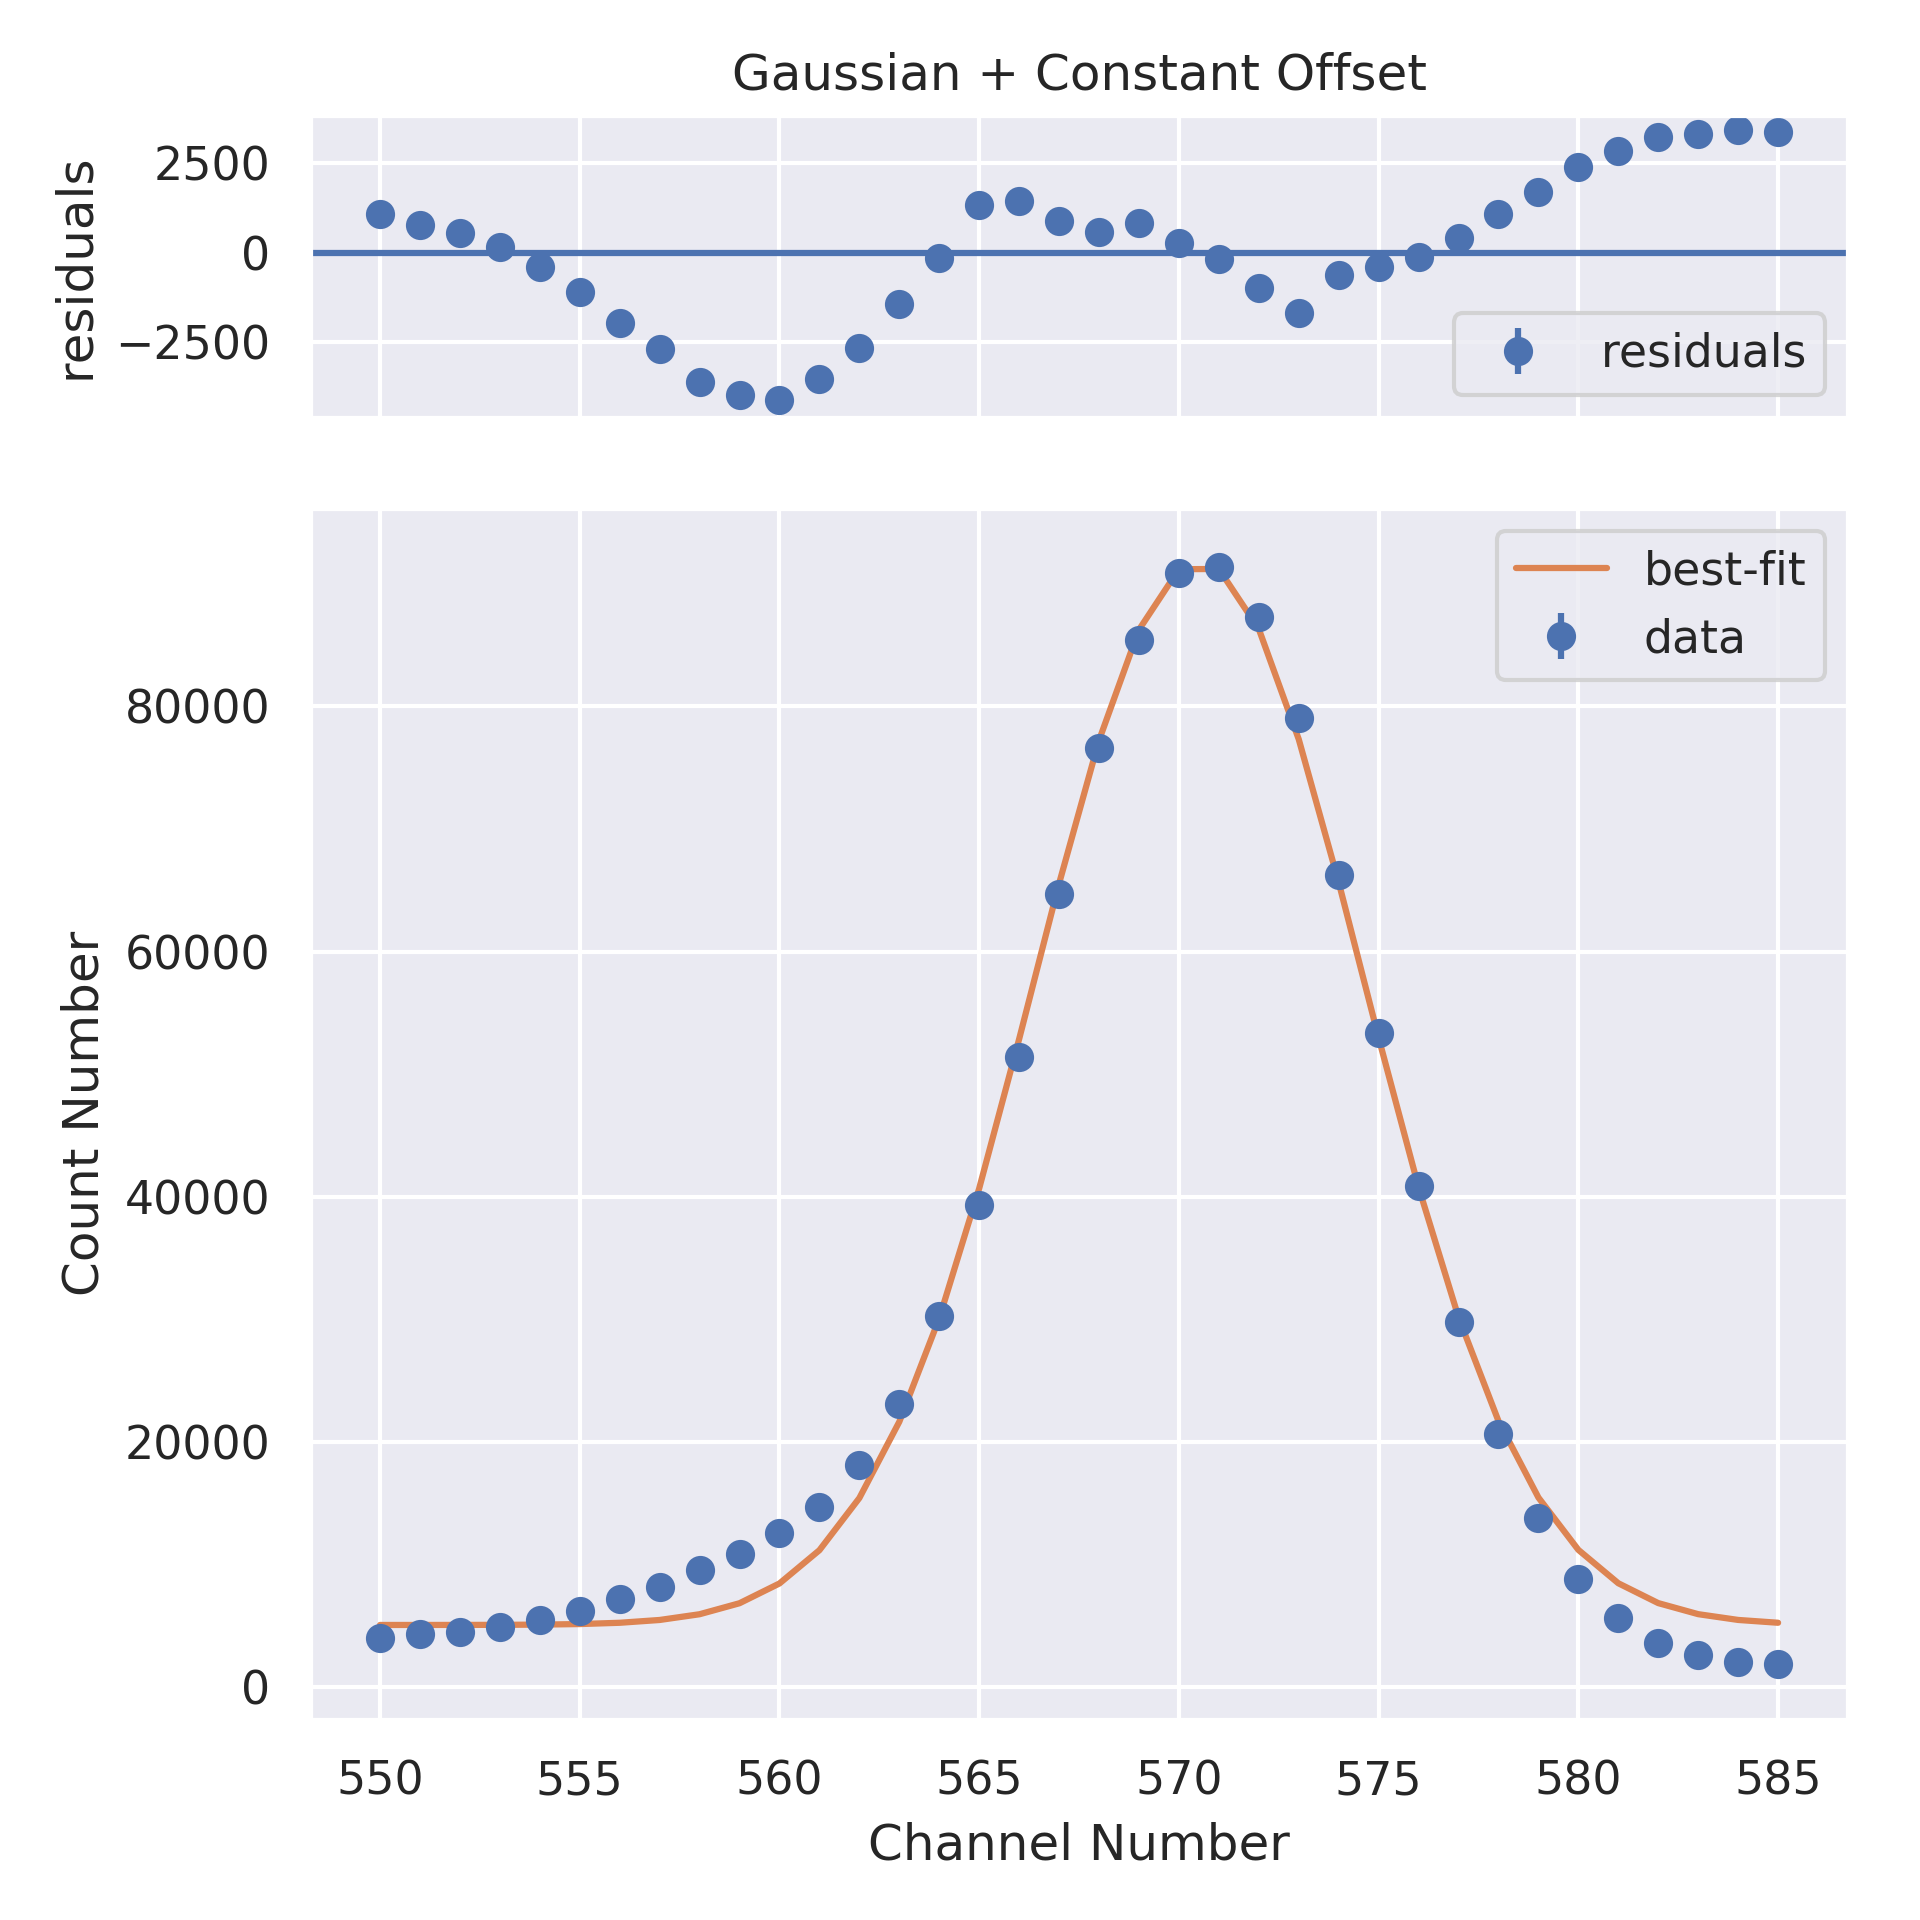
\includegraphics[width=\linewidth]{./Images/Barium133/Gauss/Gauss_1_Full.png}
    \caption{Full peak with fit}
    %\label{fig:sub1}
  \end{subfigure}%
  \begin{subfigure}{.5\linewidth}
    \centering
    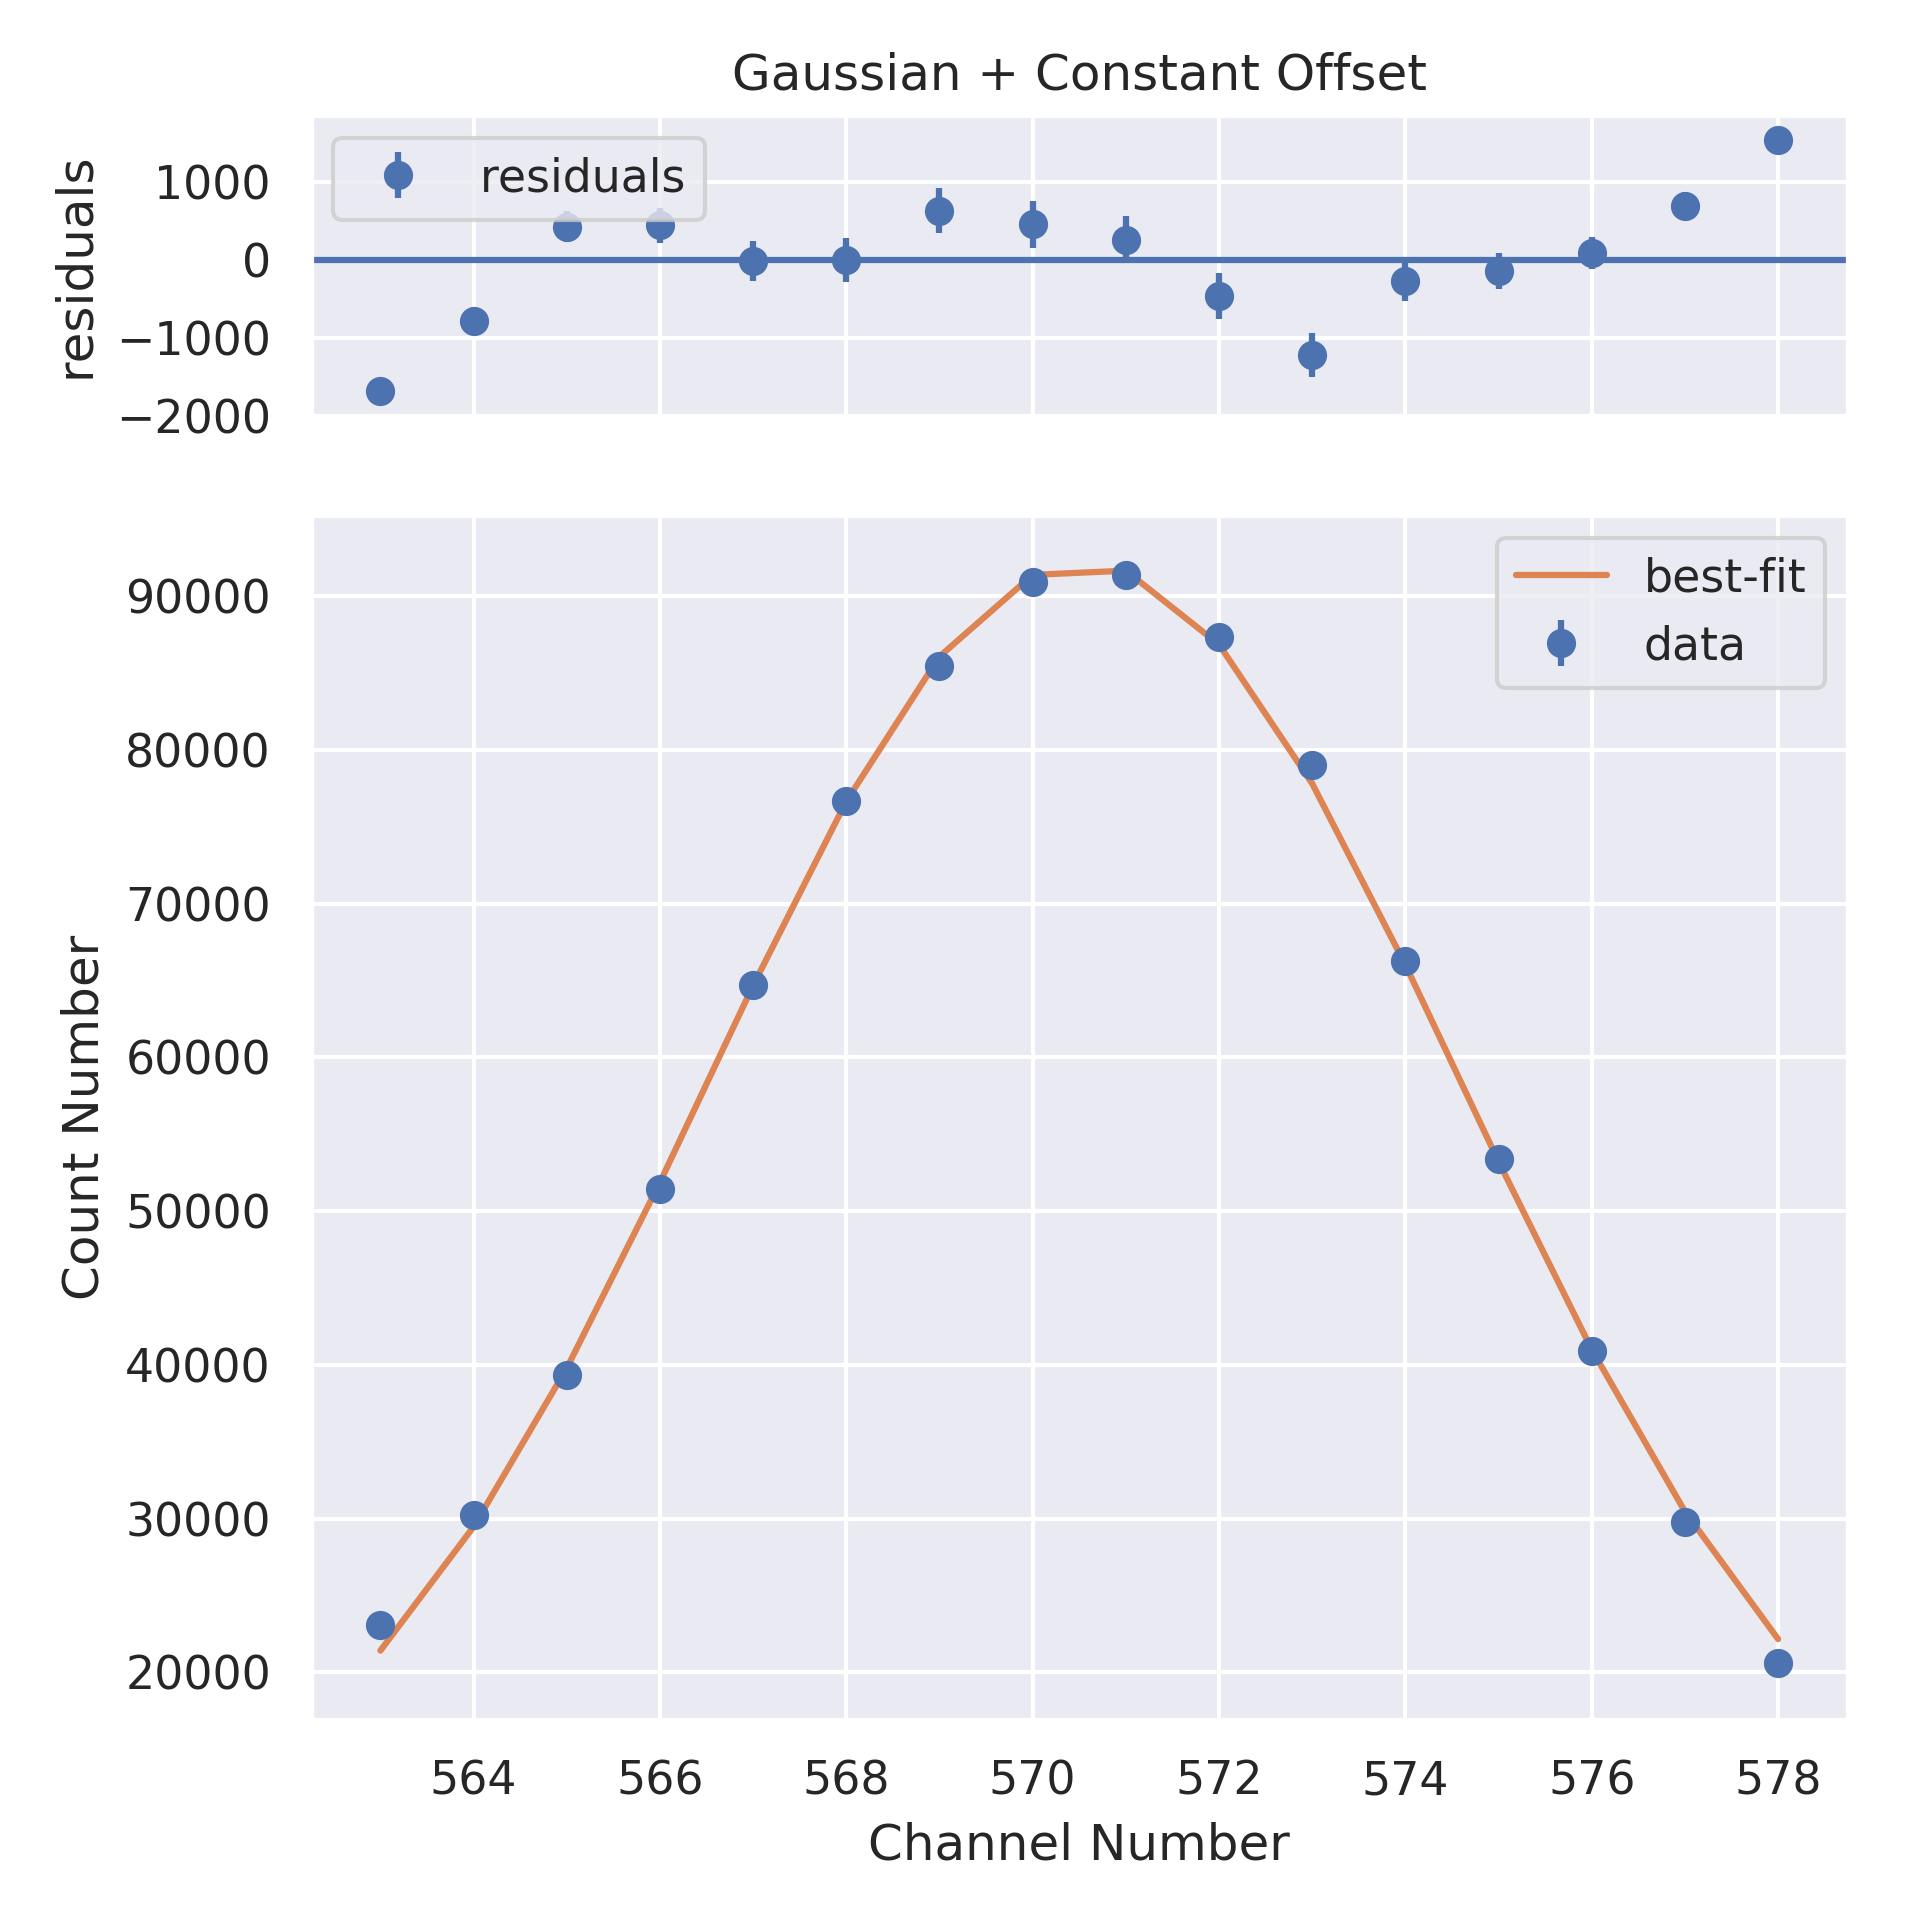
\includegraphics[width=\linewidth]{./Images/Barium133/Gauss/Gauss_1_Zoom.png}
    \caption{Zoomed in peak with fit}
    %\label{fig:sub2}
  \end{subfigure}
  \caption{Fit of full \& zoomed in peak of \element{Ba}{133} 81 keV peak}
  %\label{fig:test}
\end{figure}
\begin{figure}[H]
  \centering
  \begin{subfigure}{.5\linewidth}
    \centering
    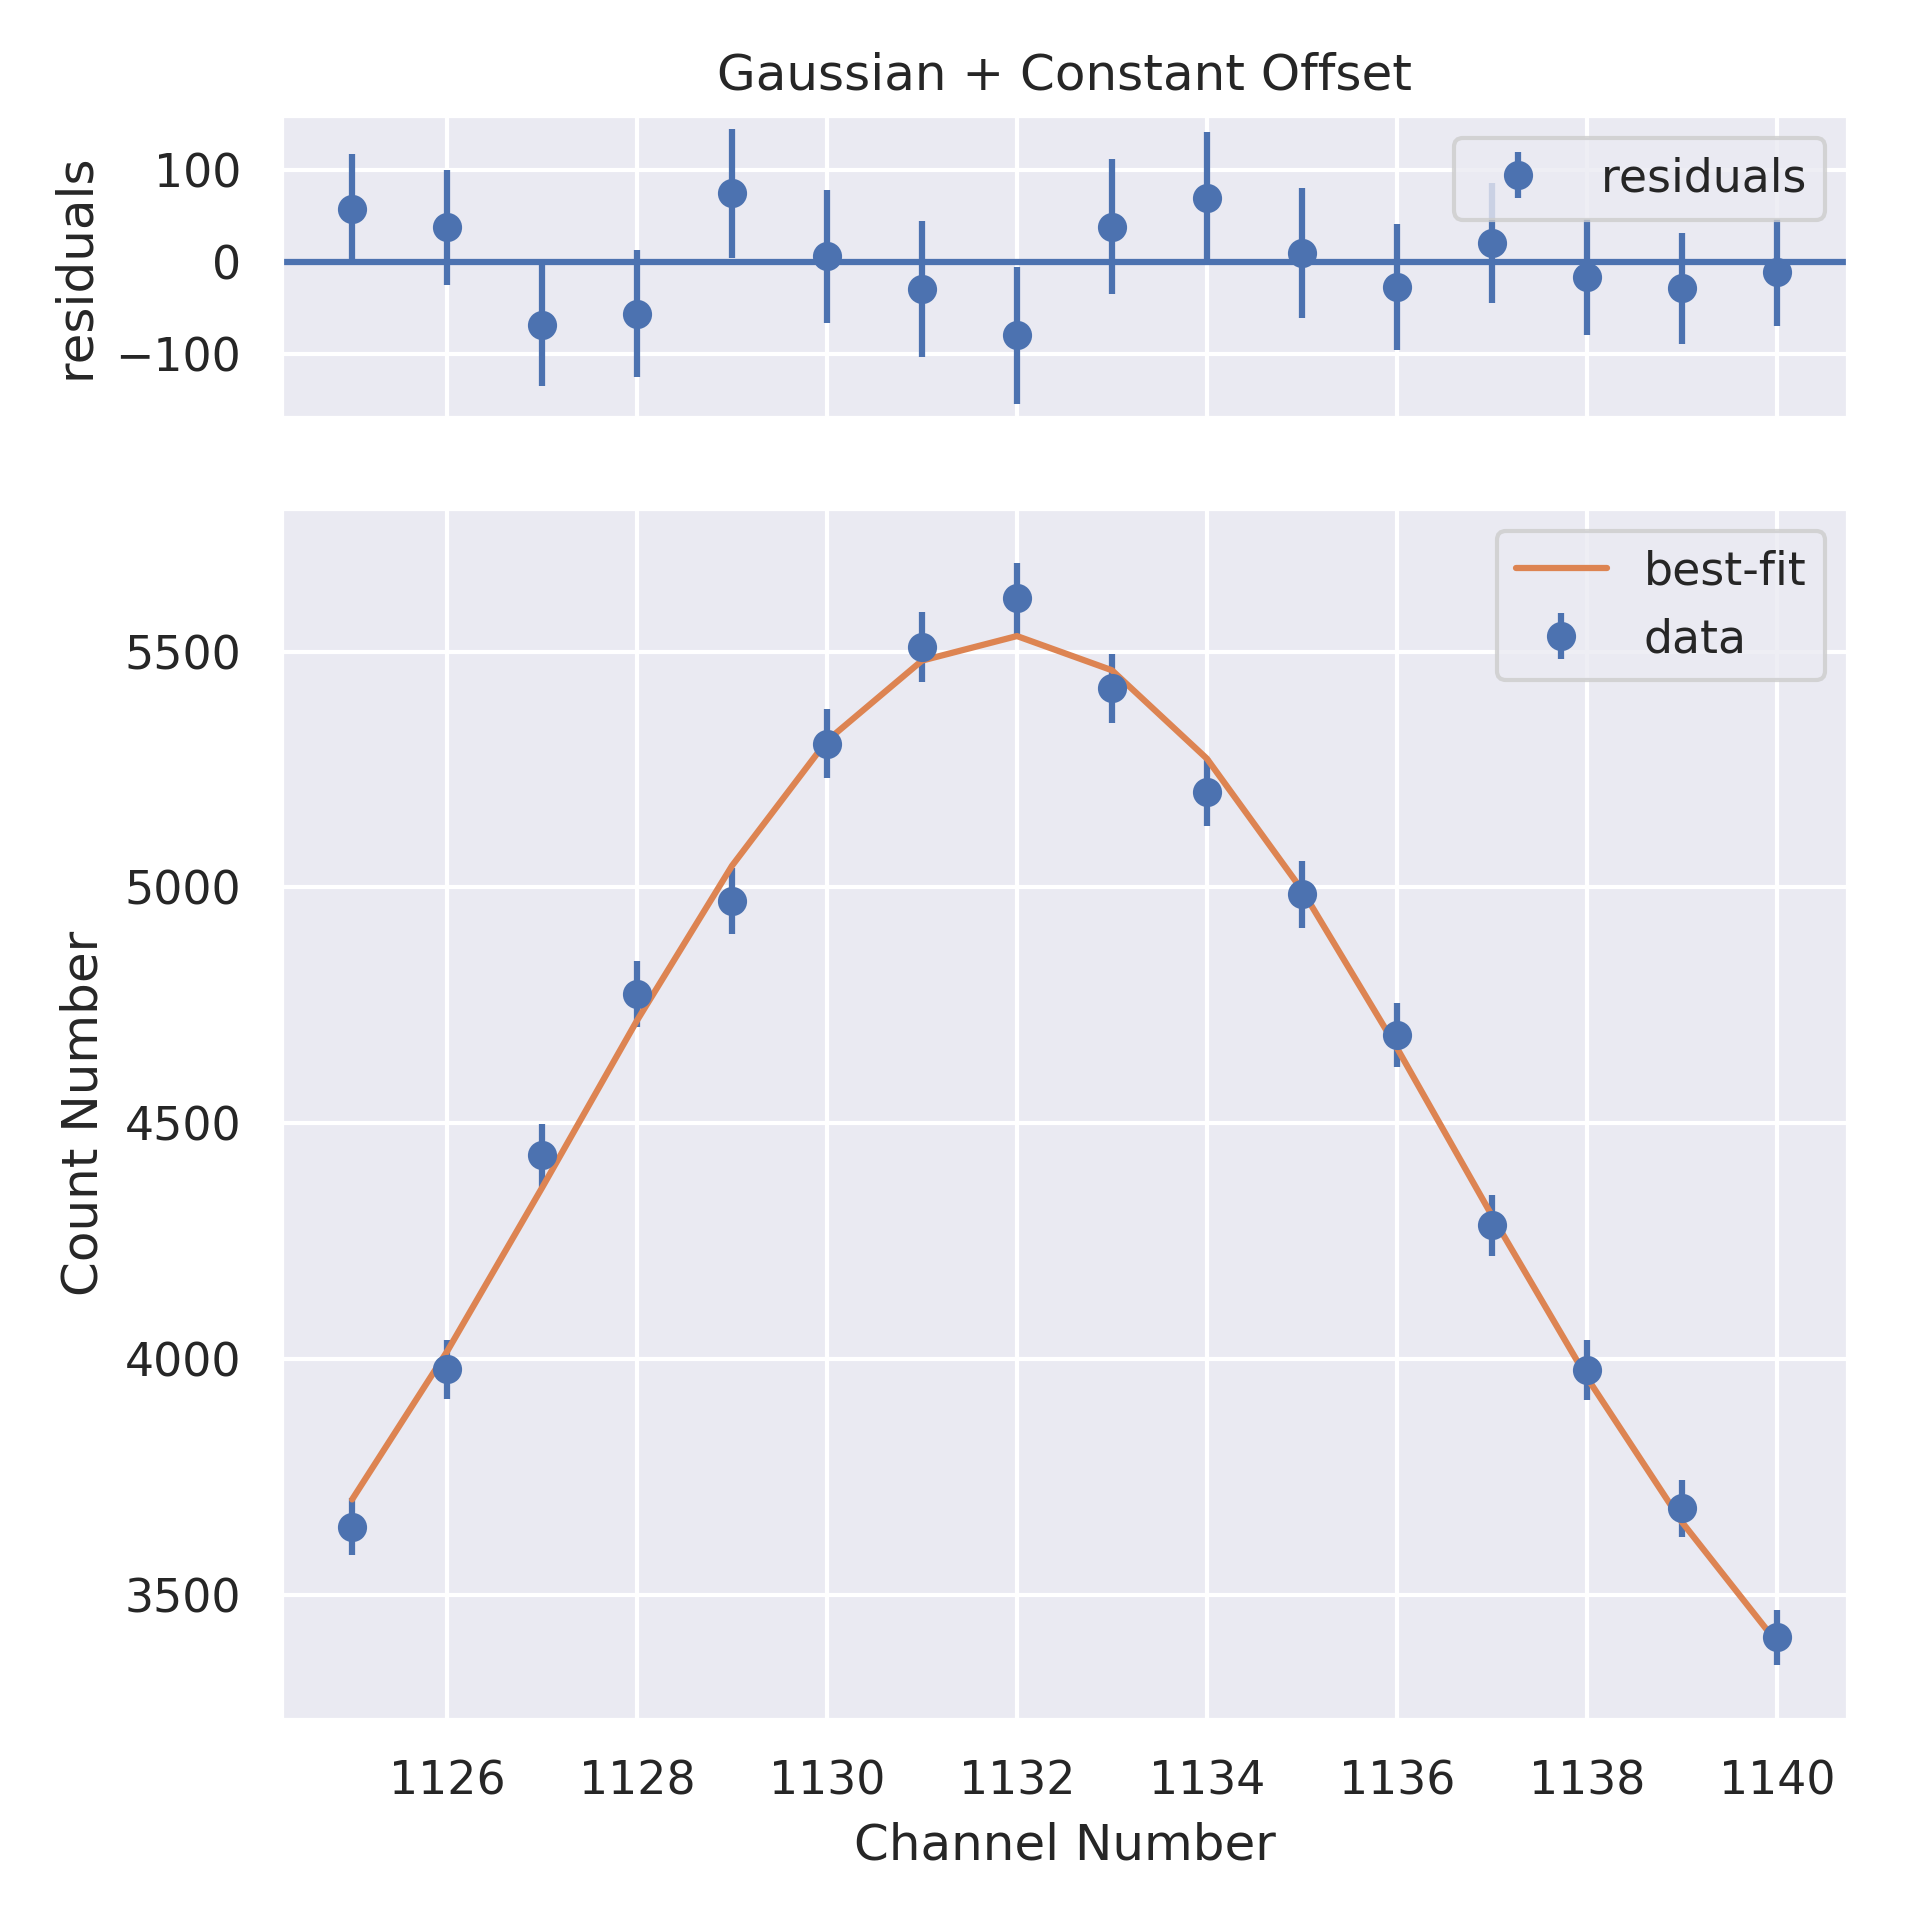
\includegraphics[width=\linewidth]{./Images/Barium133/Gauss/Gauss_2_Full.png}
    \caption{Full peak with fit}
    %\label{fig:sub1}
  \end{subfigure}%
  \begin{subfigure}{.5\linewidth}
    \centering
    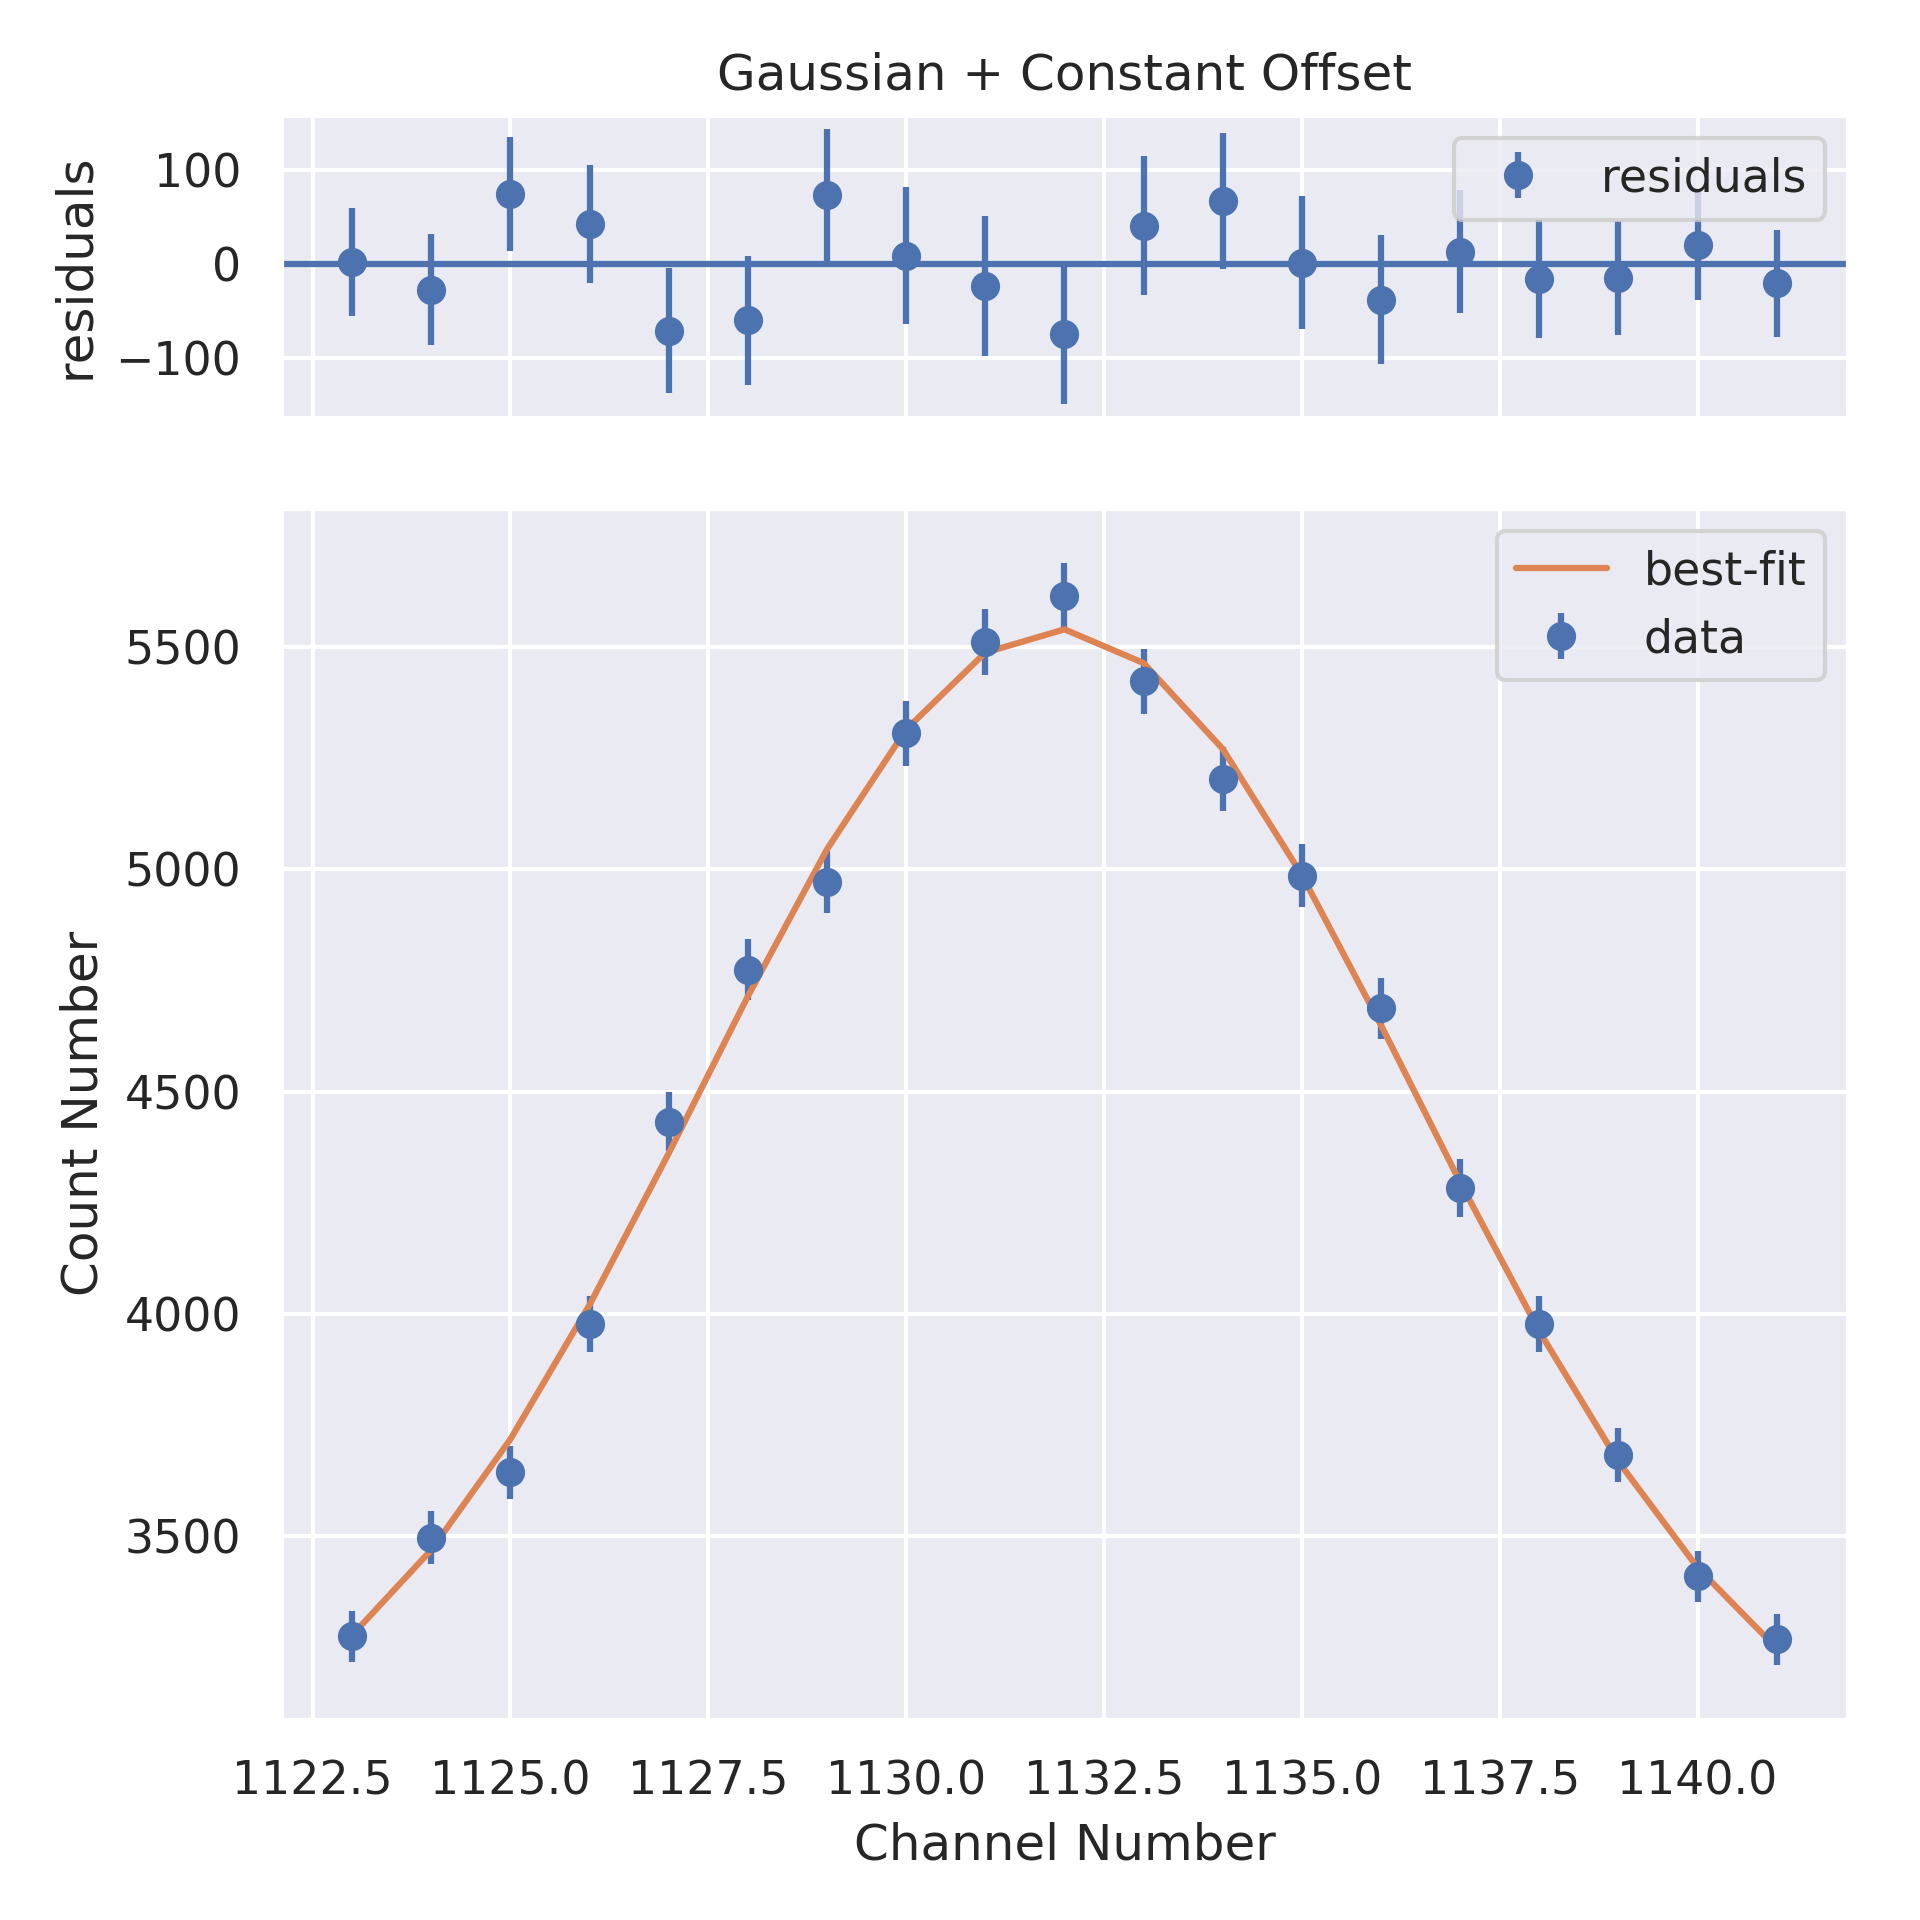
\includegraphics[width=\linewidth]{./Images/Barium133/Gauss/Gauss_2_Zoom.png}
    \caption{Zoomed in peak with fit}
    %\label{fig:sub2}
  \end{subfigure}
  \caption{Fit of full \& zoomed in peak of \element{Ba}{133} 161 keV peak}
  %\label{fig:test}
\end{figure}
\begin{figure}[H]
  \centering
  \begin{subfigure}{.5\linewidth}
    \centering
    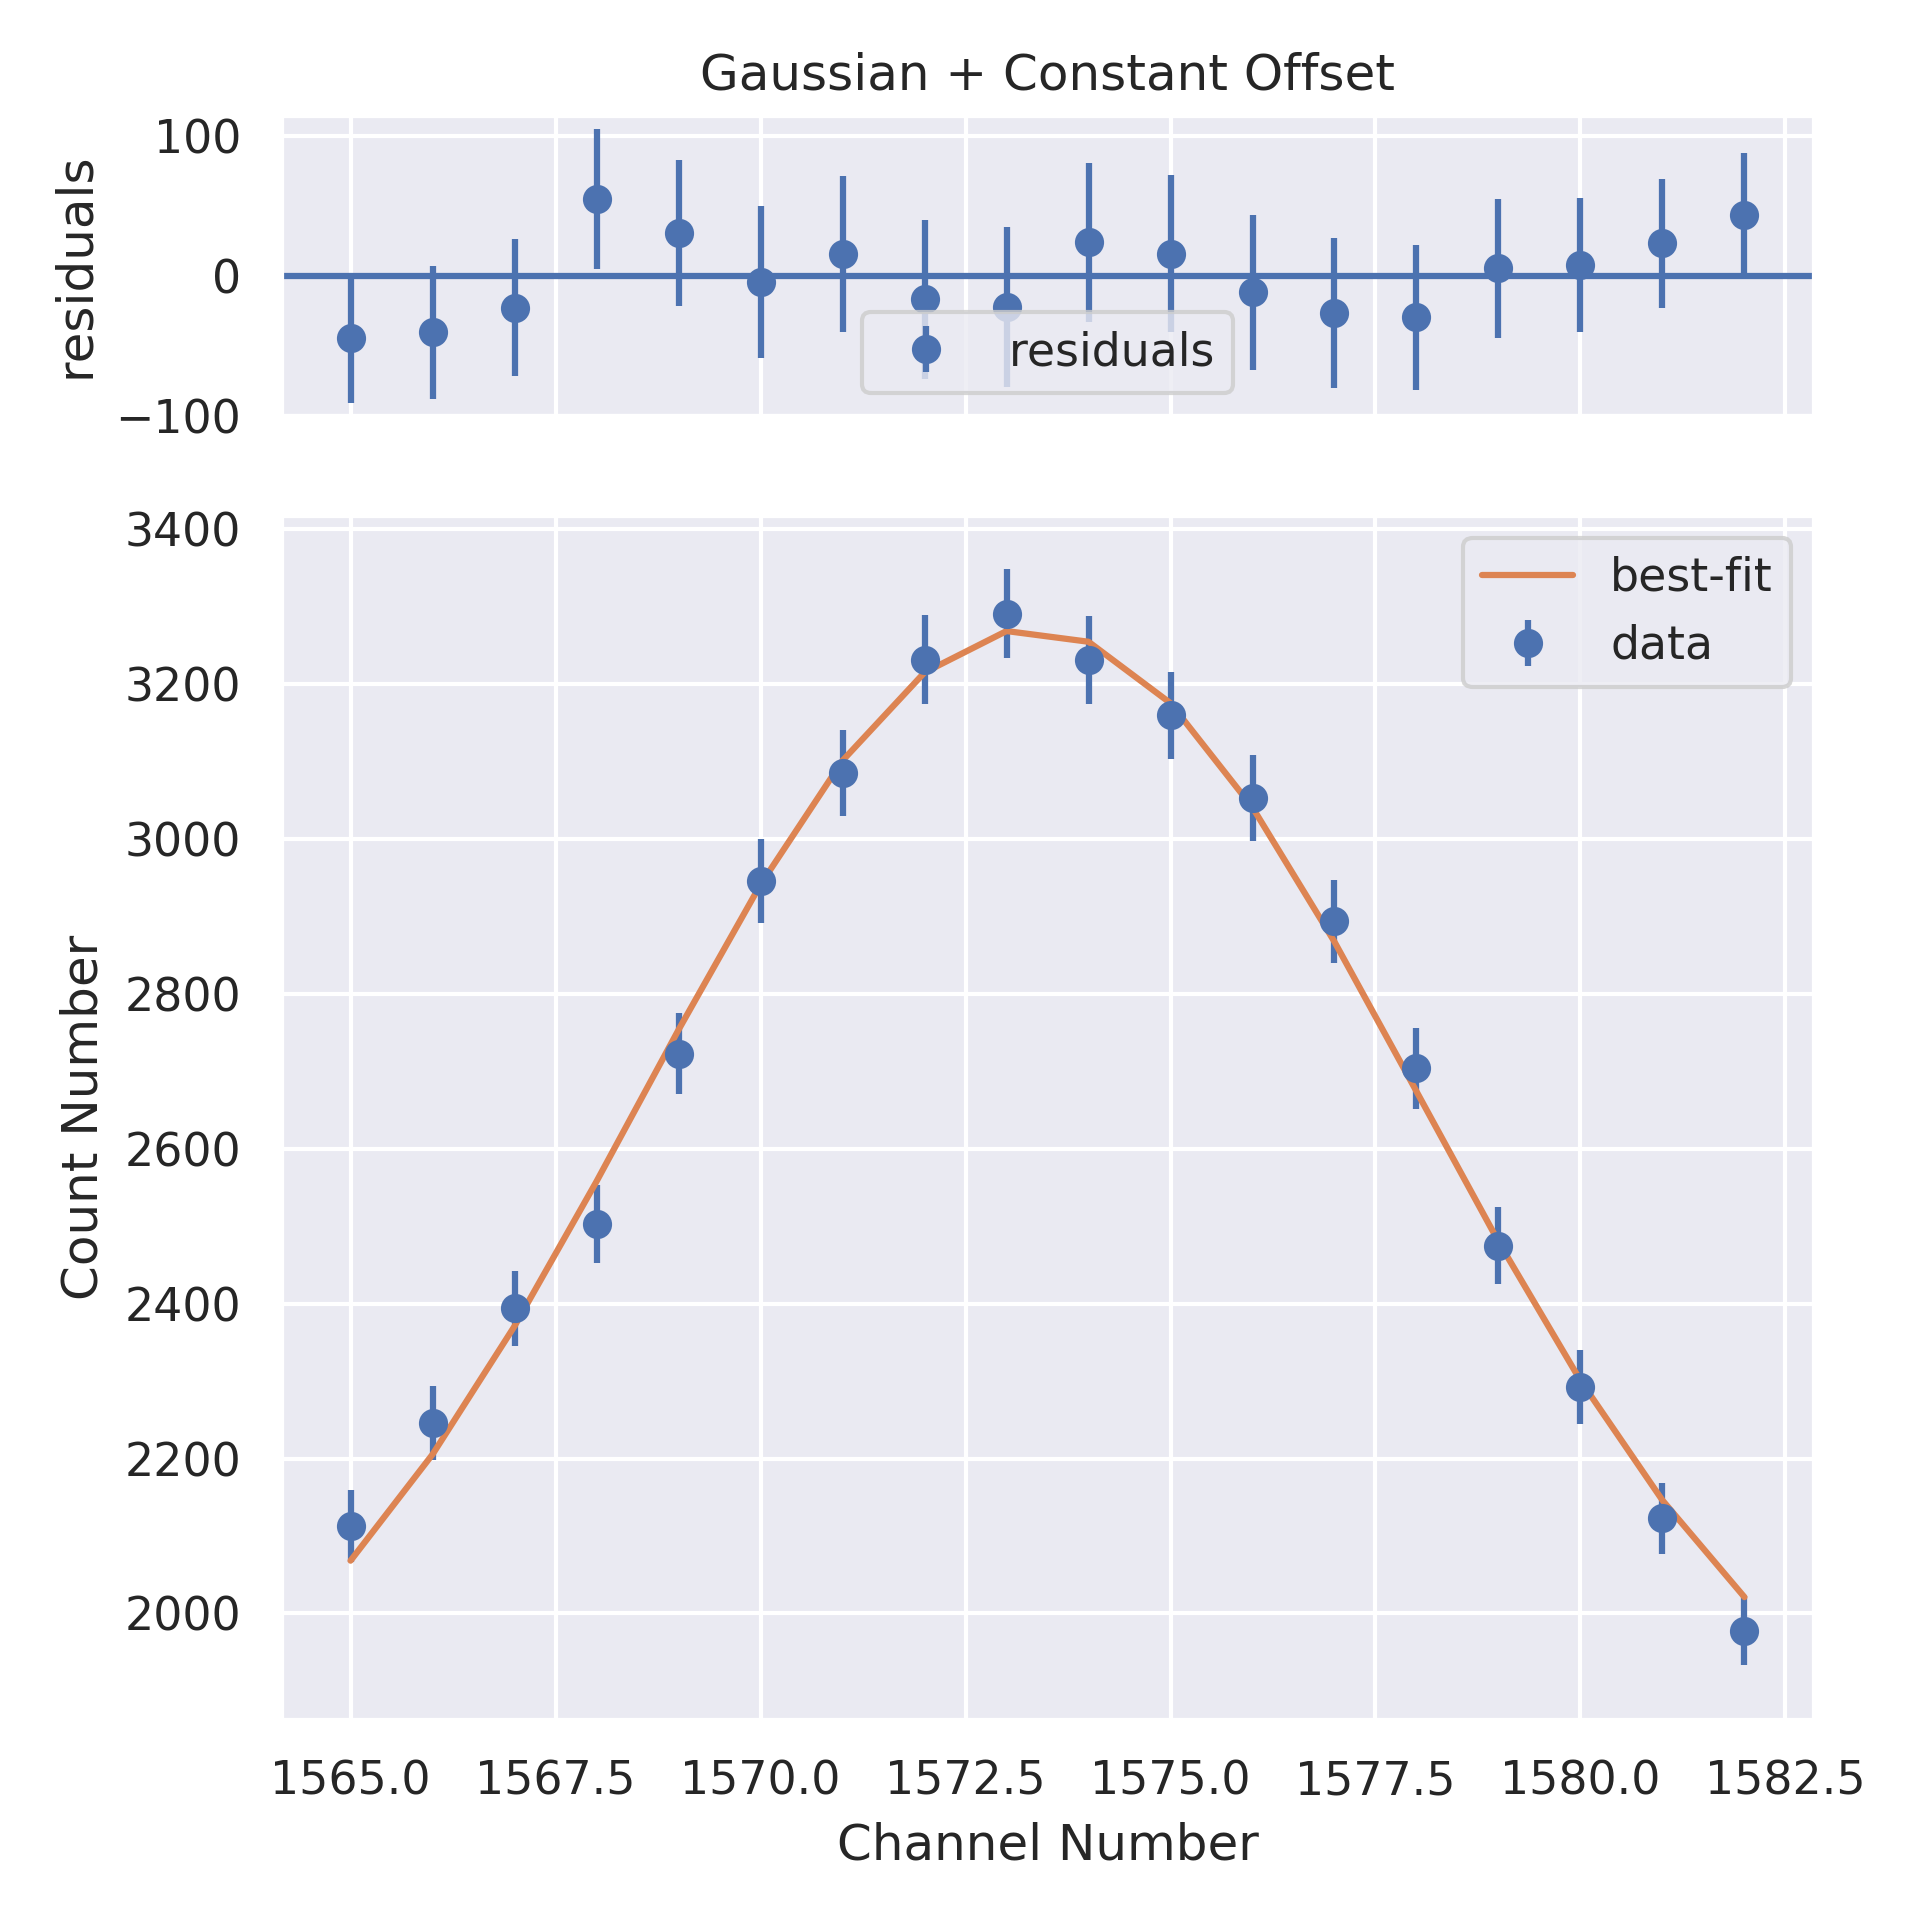
\includegraphics[width=\linewidth]{./Images/Barium133/Gauss/Gauss_3_Full.png}
    \caption{Full peak with fit}
    %\label{fig:sub1}
  \end{subfigure}%
  \begin{subfigure}{.5\linewidth}
    \centering
    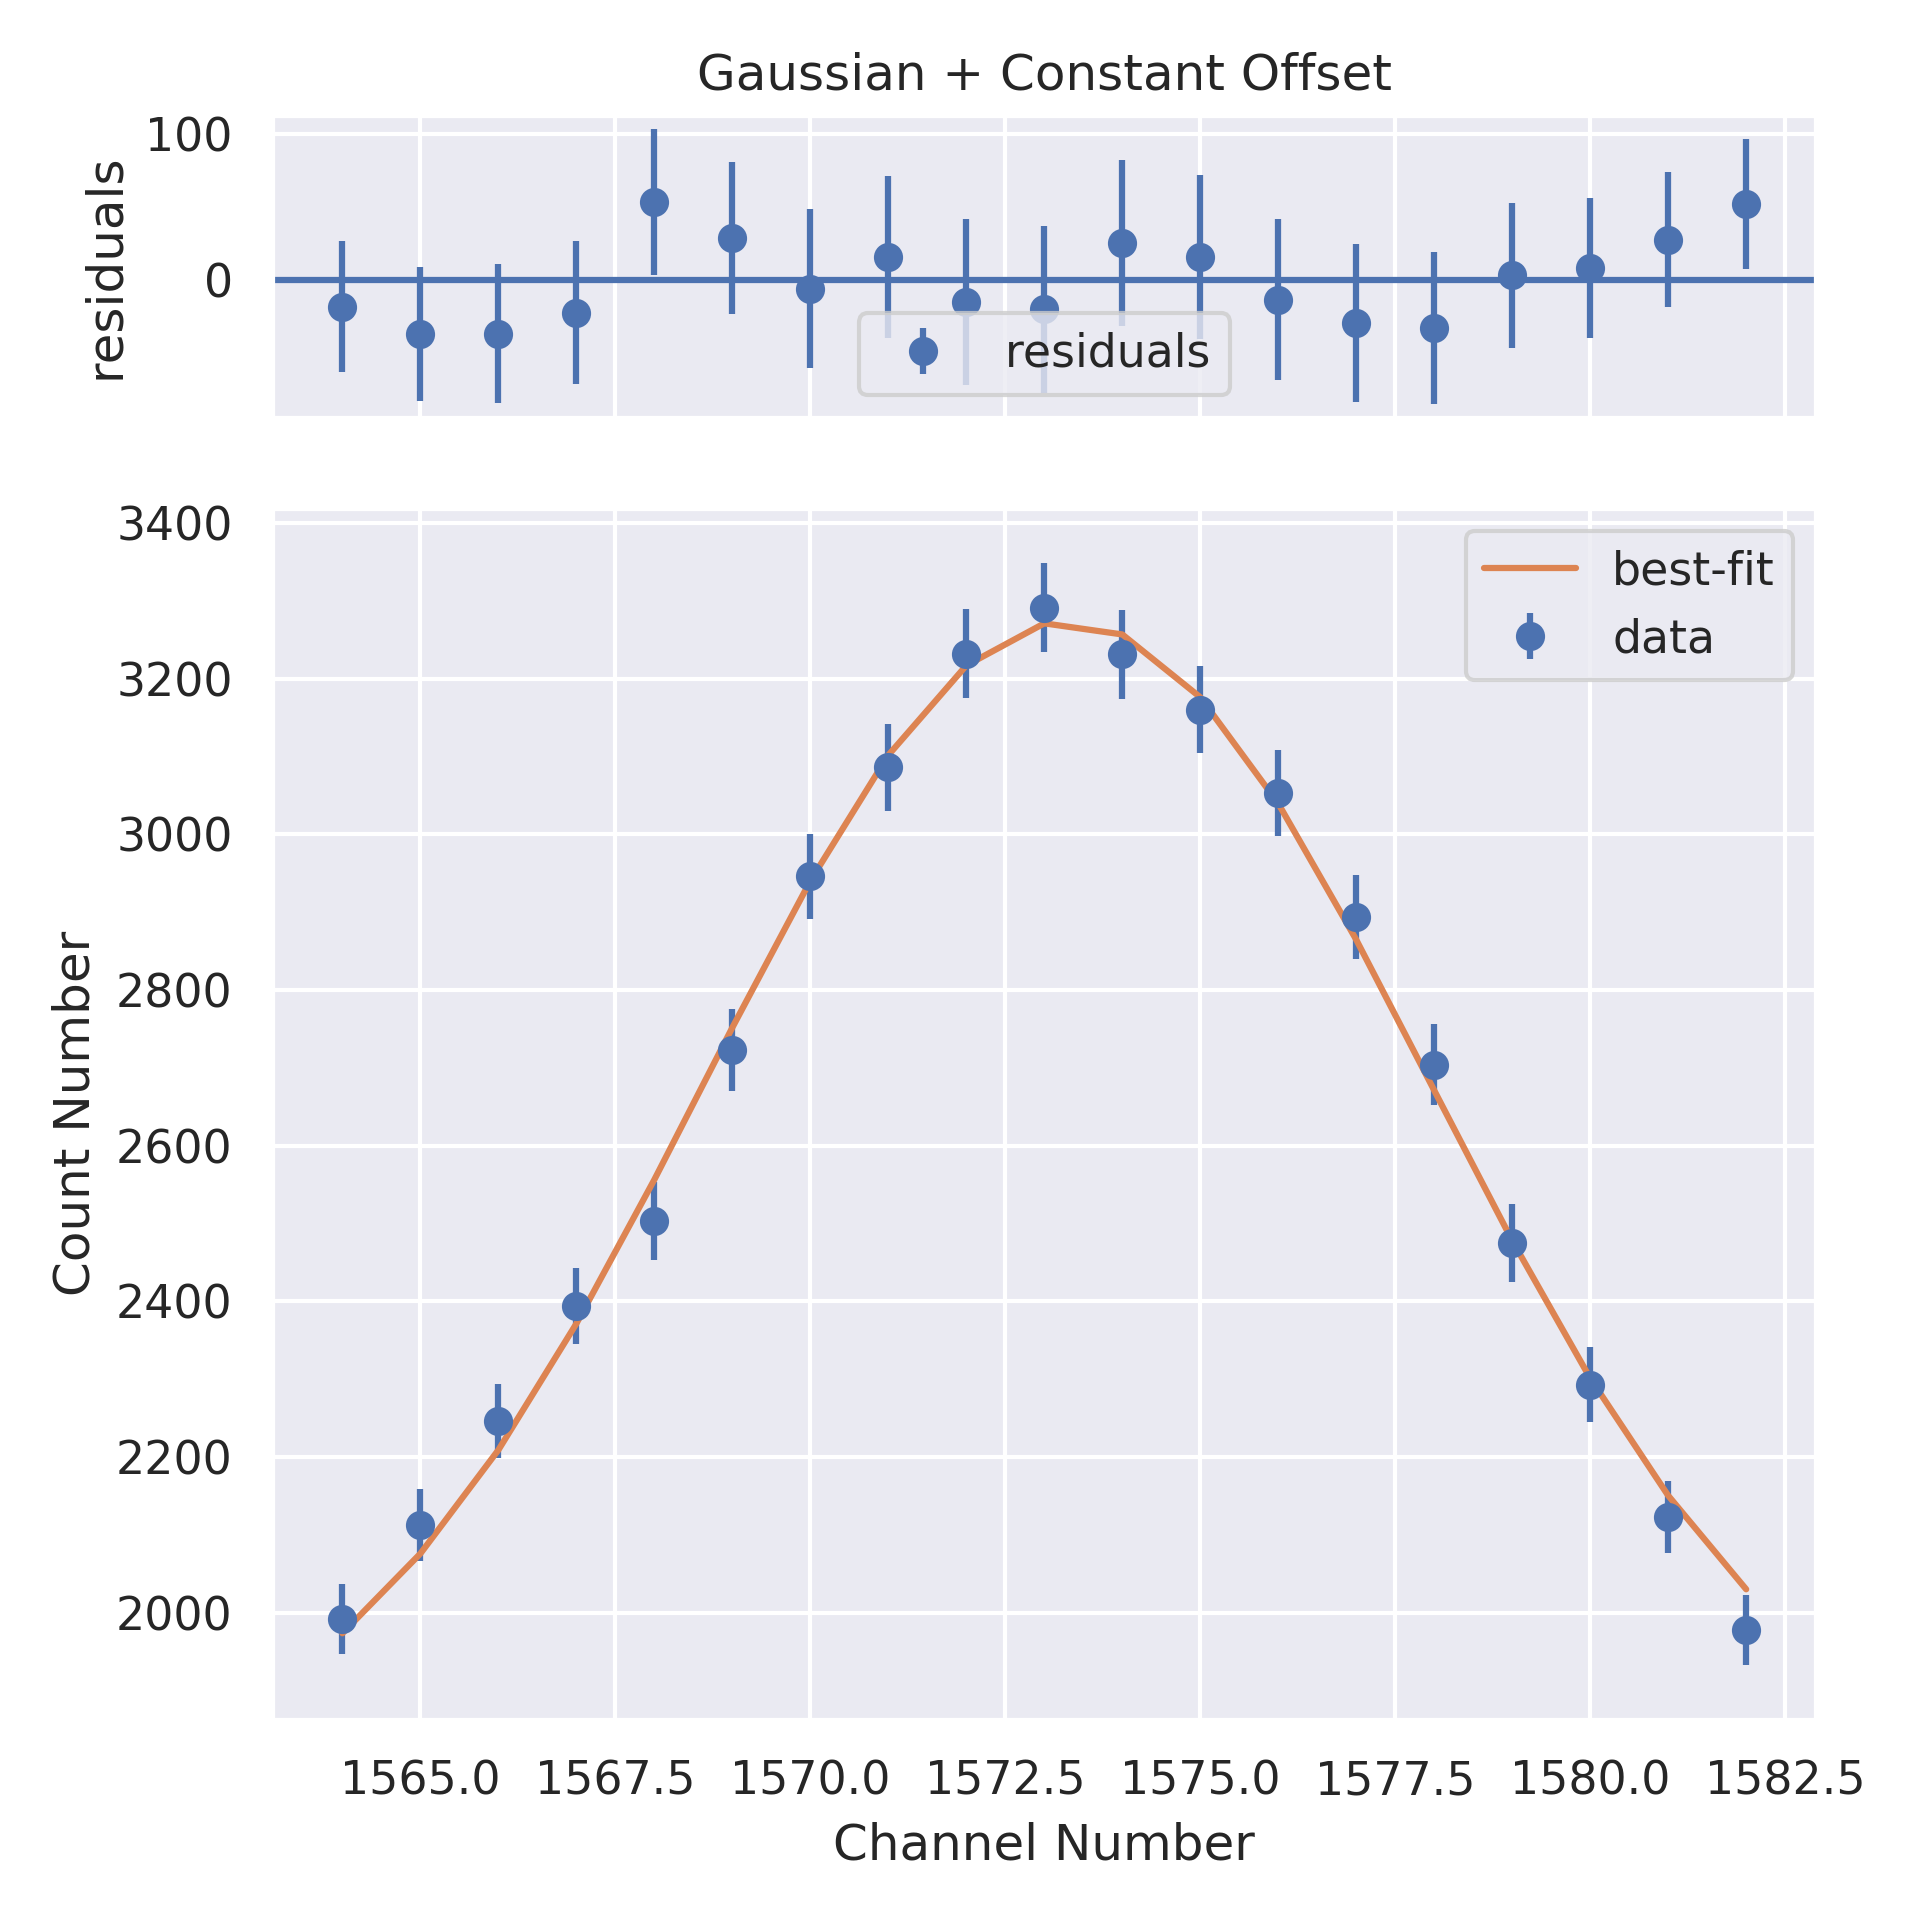
\includegraphics[width=\linewidth]{./Images/Barium133/Gauss/Gauss_3_Zoom.png}
    \caption{Zoomed in peak with fit}
    %\label{fig:sub2}
  \end{subfigure}
  \caption{Fit of full \& zoomed in peak of \element{Ba}{133} 223 keV peak}
  %\label{fig:test}
\end{figure}
\begin{figure}[H]
  \centering
  \begin{subfigure}{.5\linewidth}
    \centering
    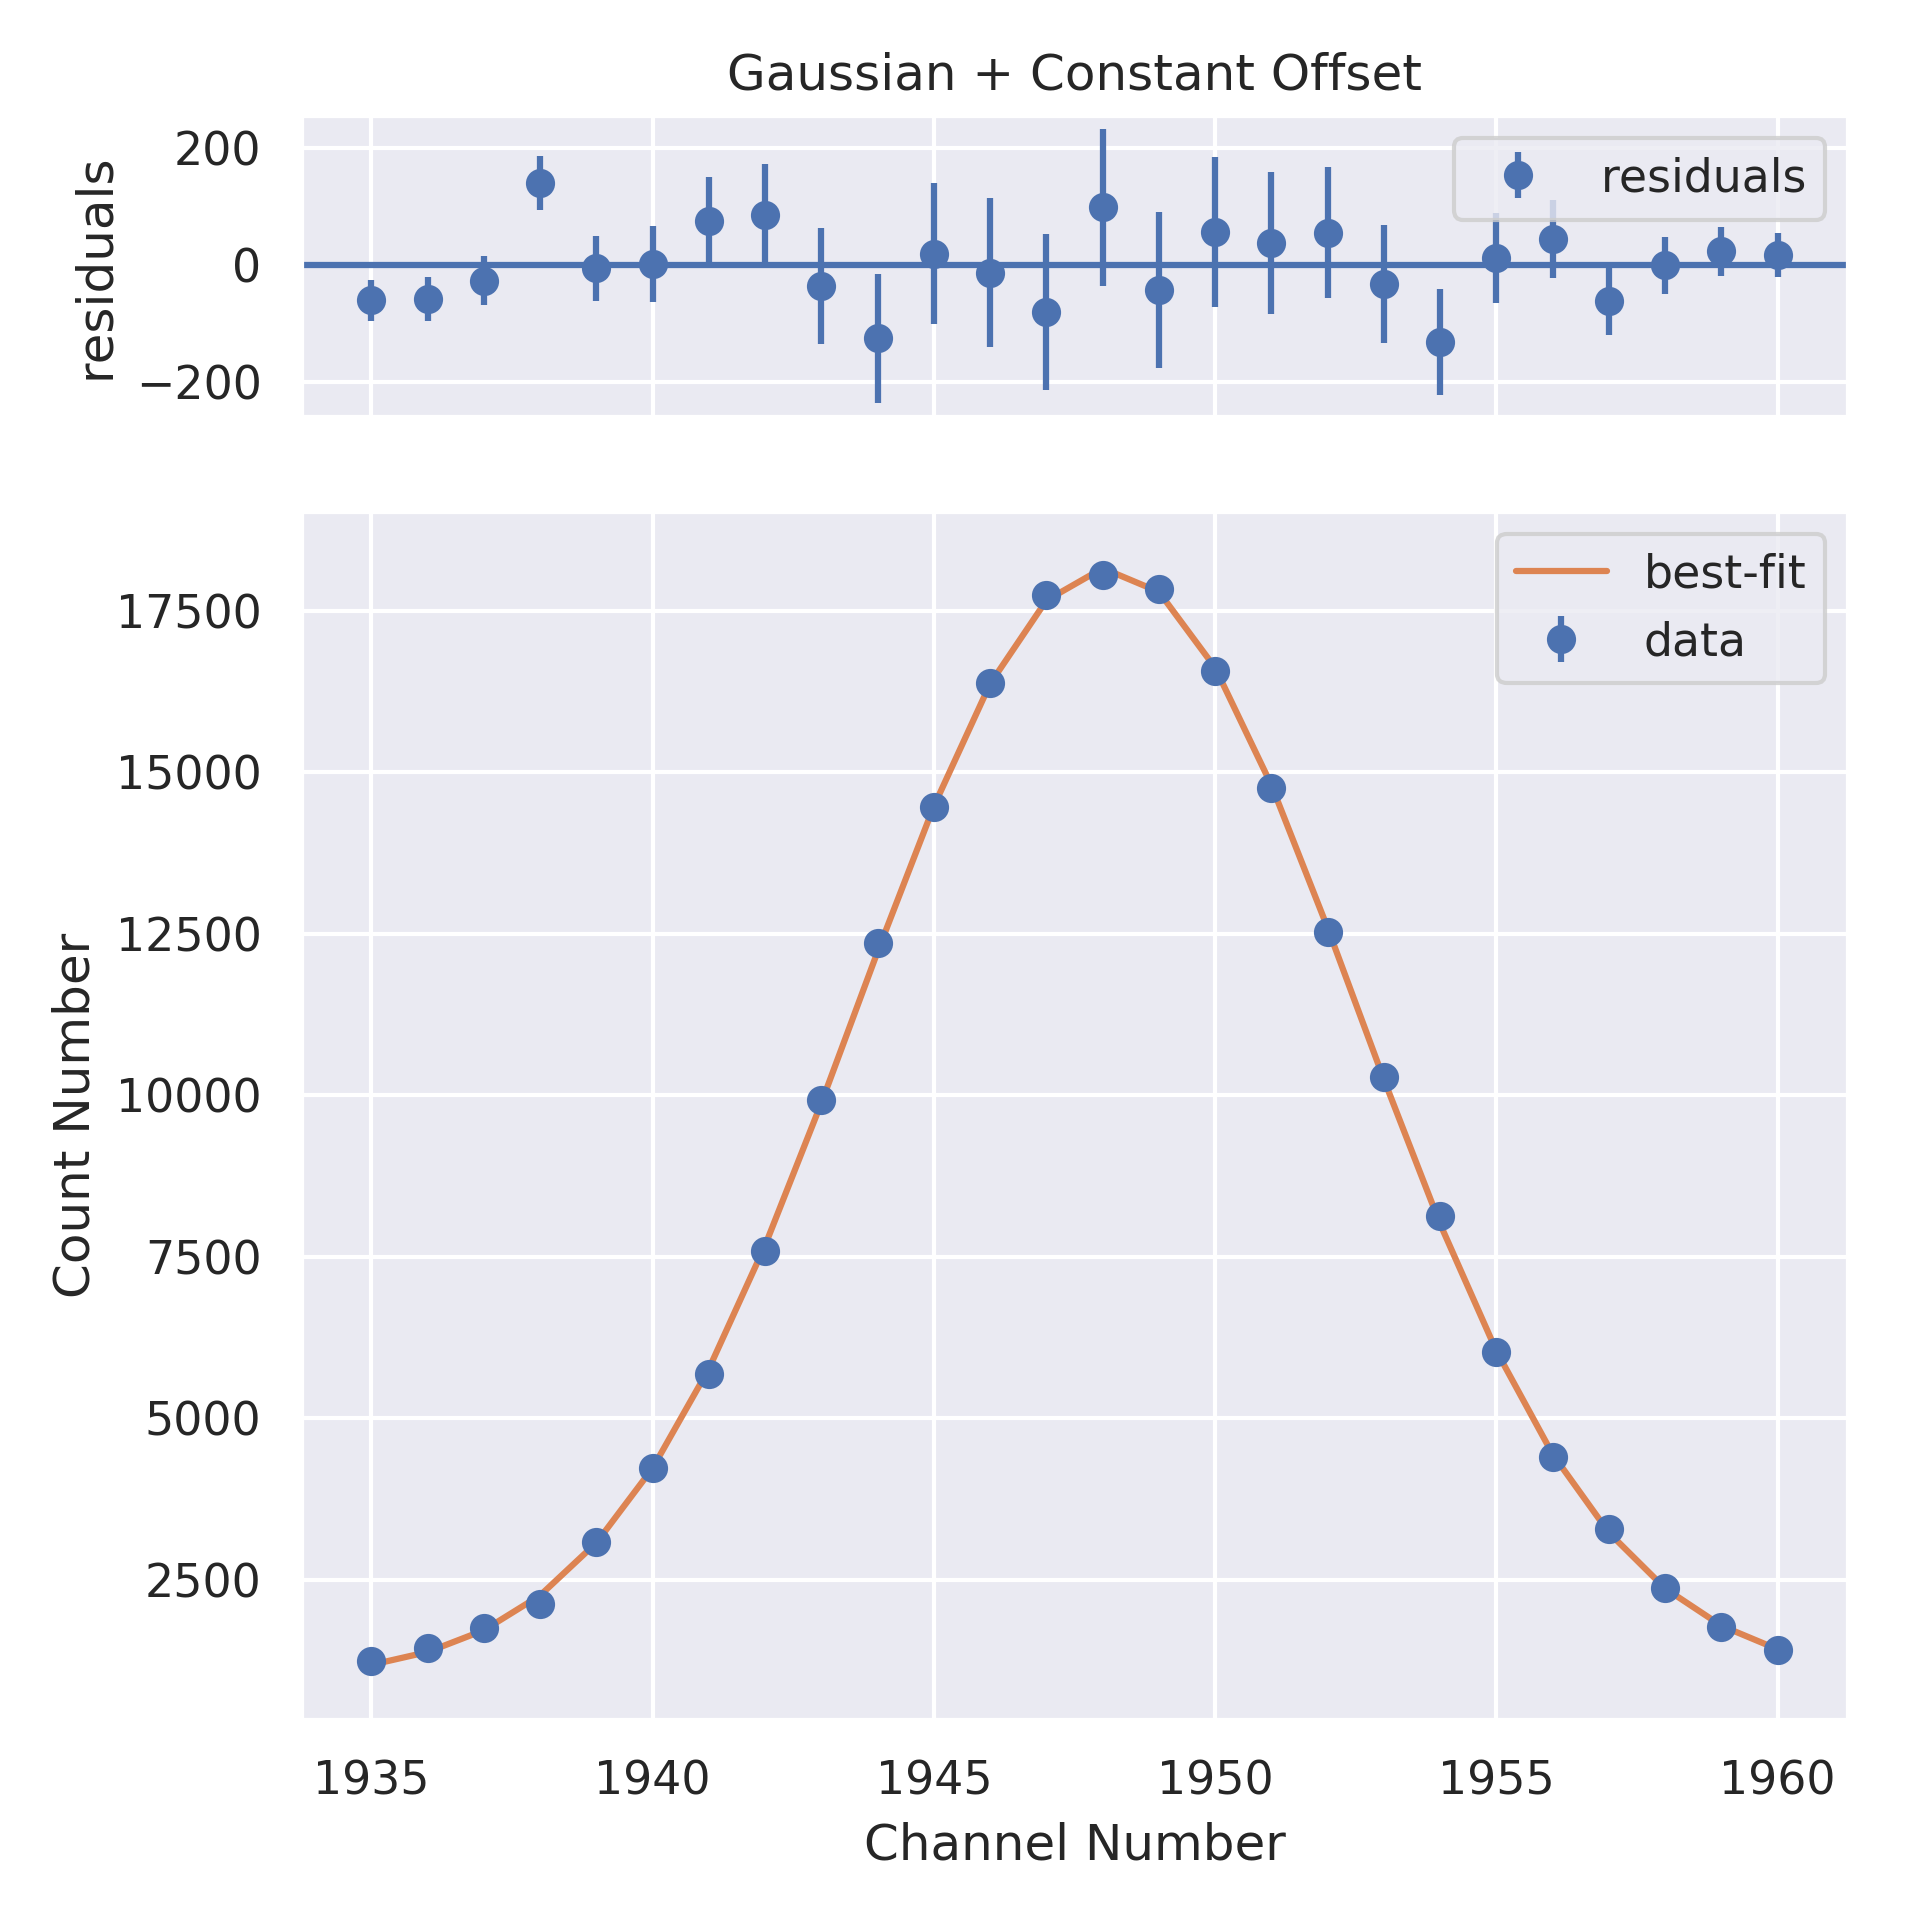
\includegraphics[width=\linewidth]{./Images/Barium133/Gauss/Gauss_4_Full.png}
    \caption{Full peak with fit}
    %\label{fig:sub1}
  \end{subfigure}%
  \begin{subfigure}{.5\linewidth}
    \centering
    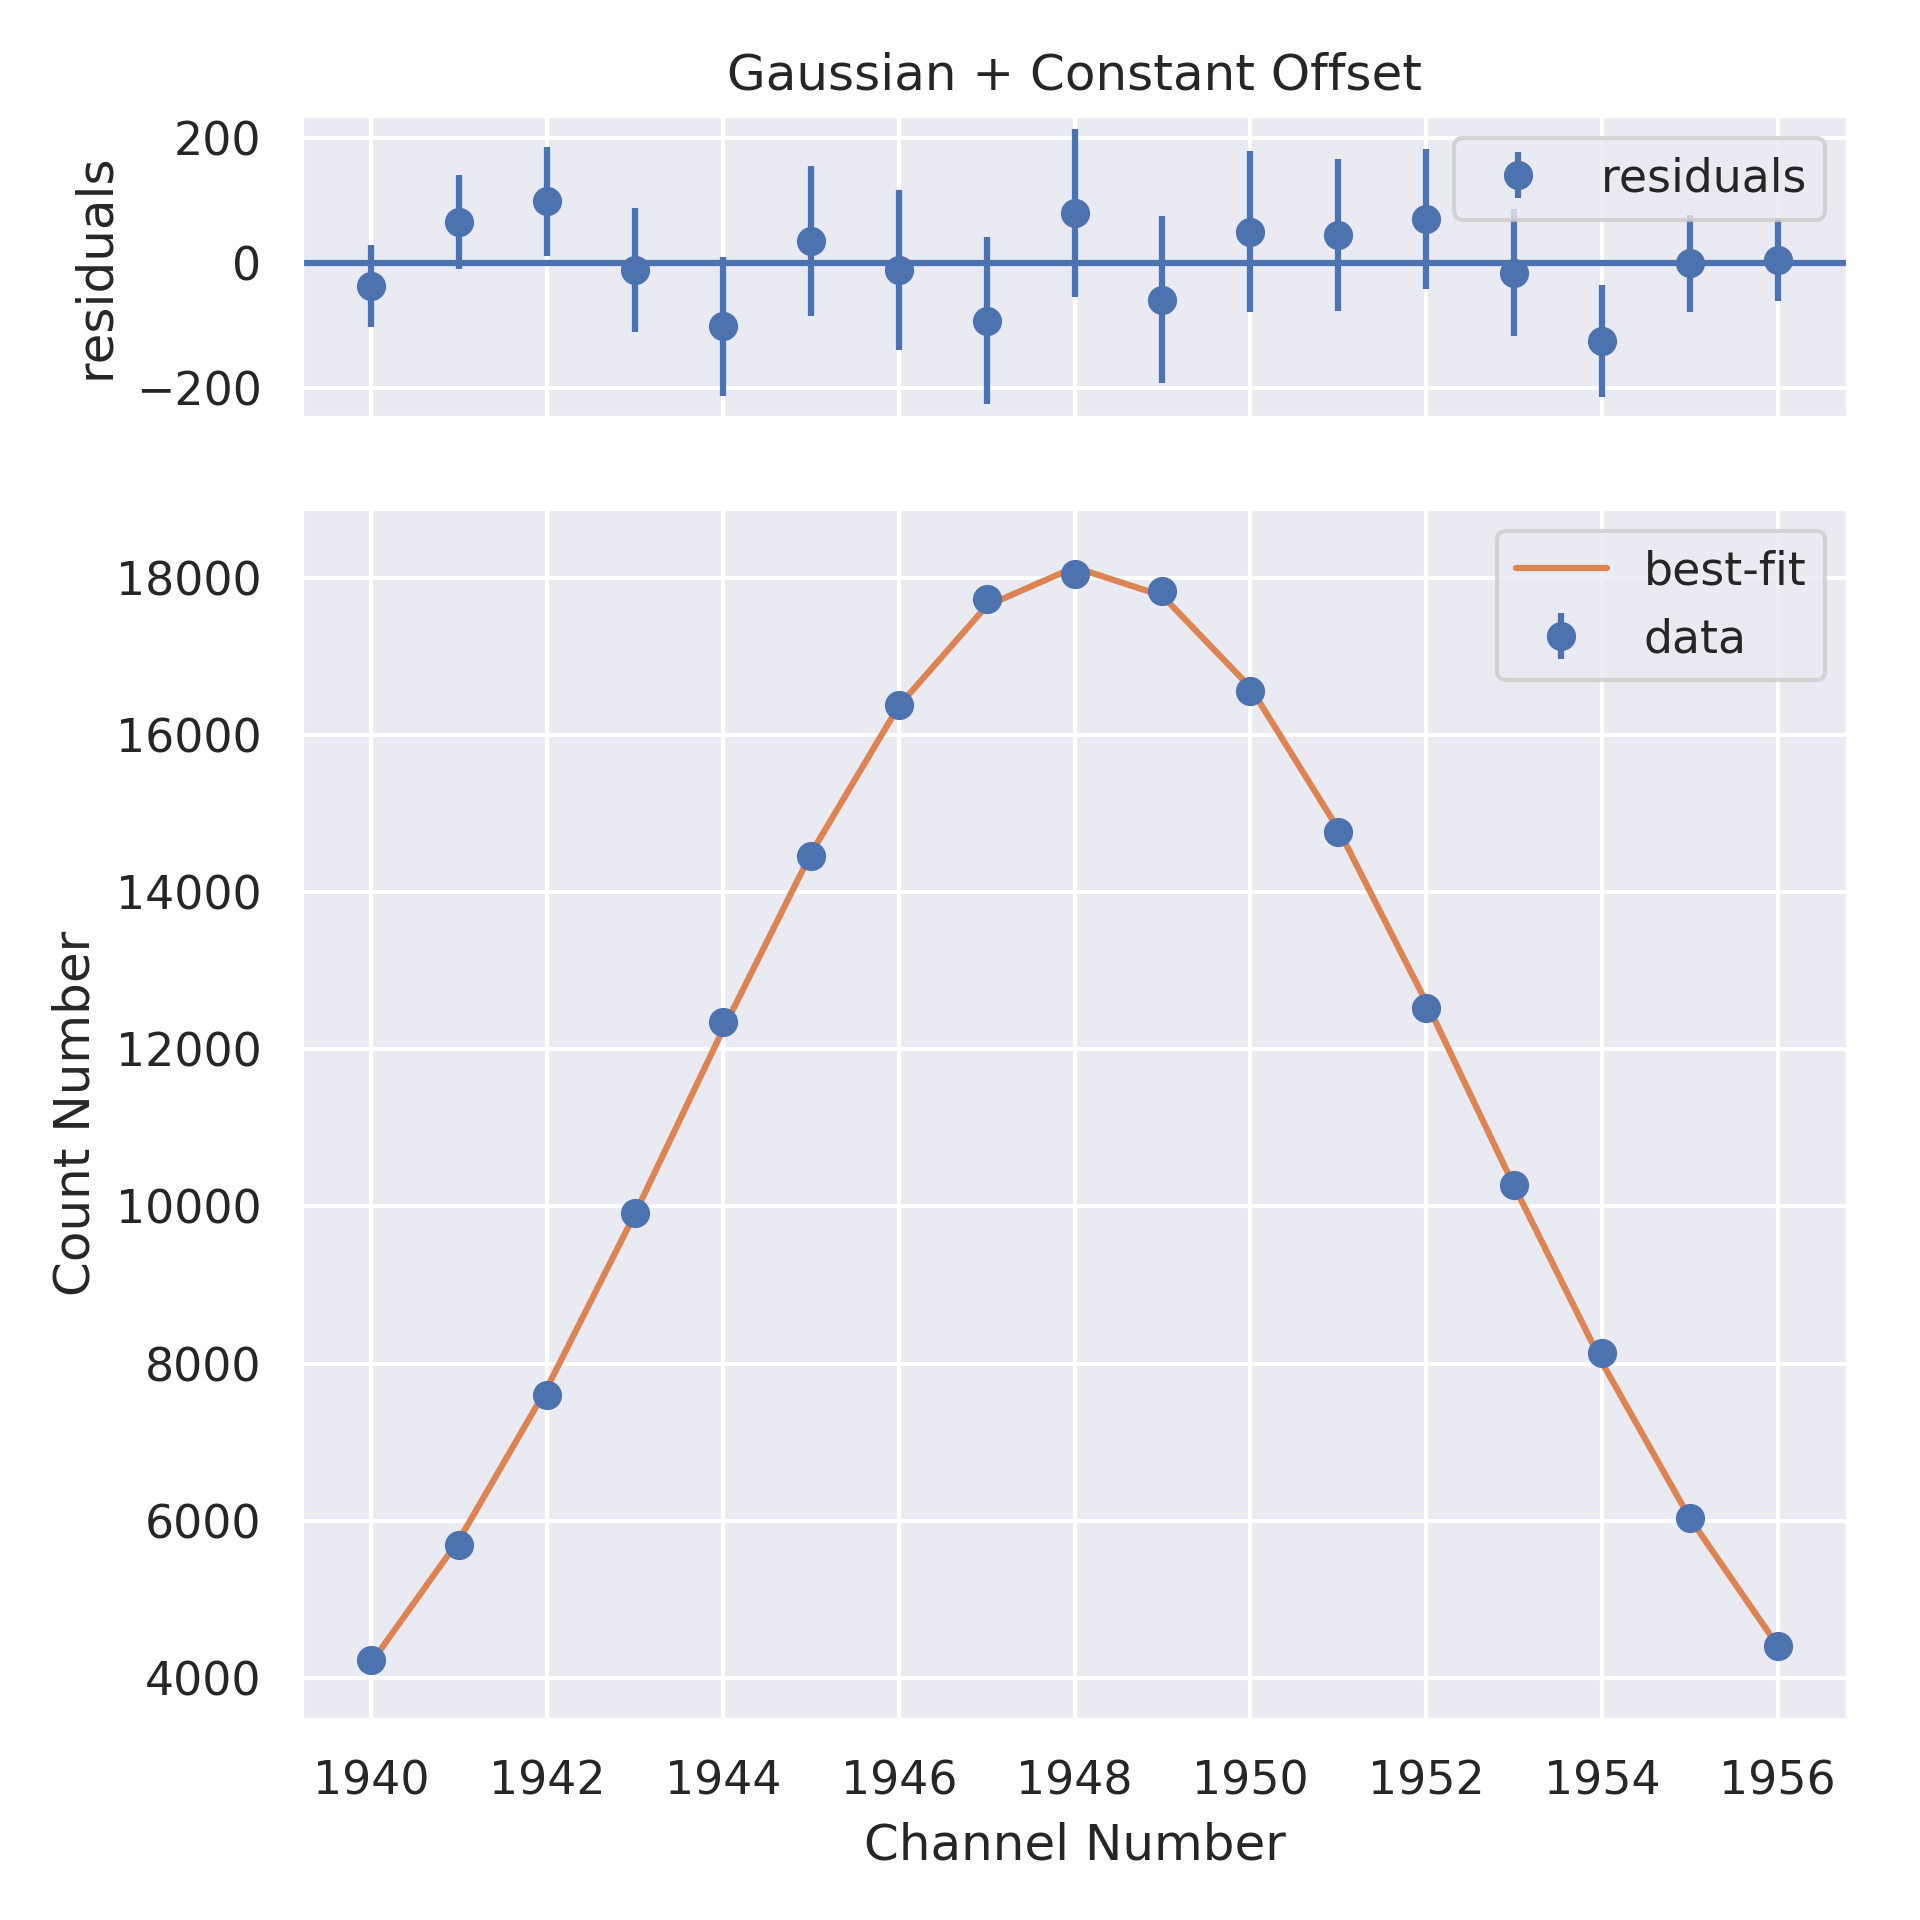
\includegraphics[width=\linewidth]{./Images/Barium133/Gauss/Gauss_4_Zoom.png}
    \caption{Zoomed in peak with fit}
    %\label{fig:sub2}
  \end{subfigure}
  \caption{Fit of full \& zoomed in peak of \element{Ba}{133} 276 keV peak}
  %\label{fig:test}
\end{figure}
\begin{figure}[H]
  \centering
  \begin{subfigure}{.5\linewidth}
    \centering
    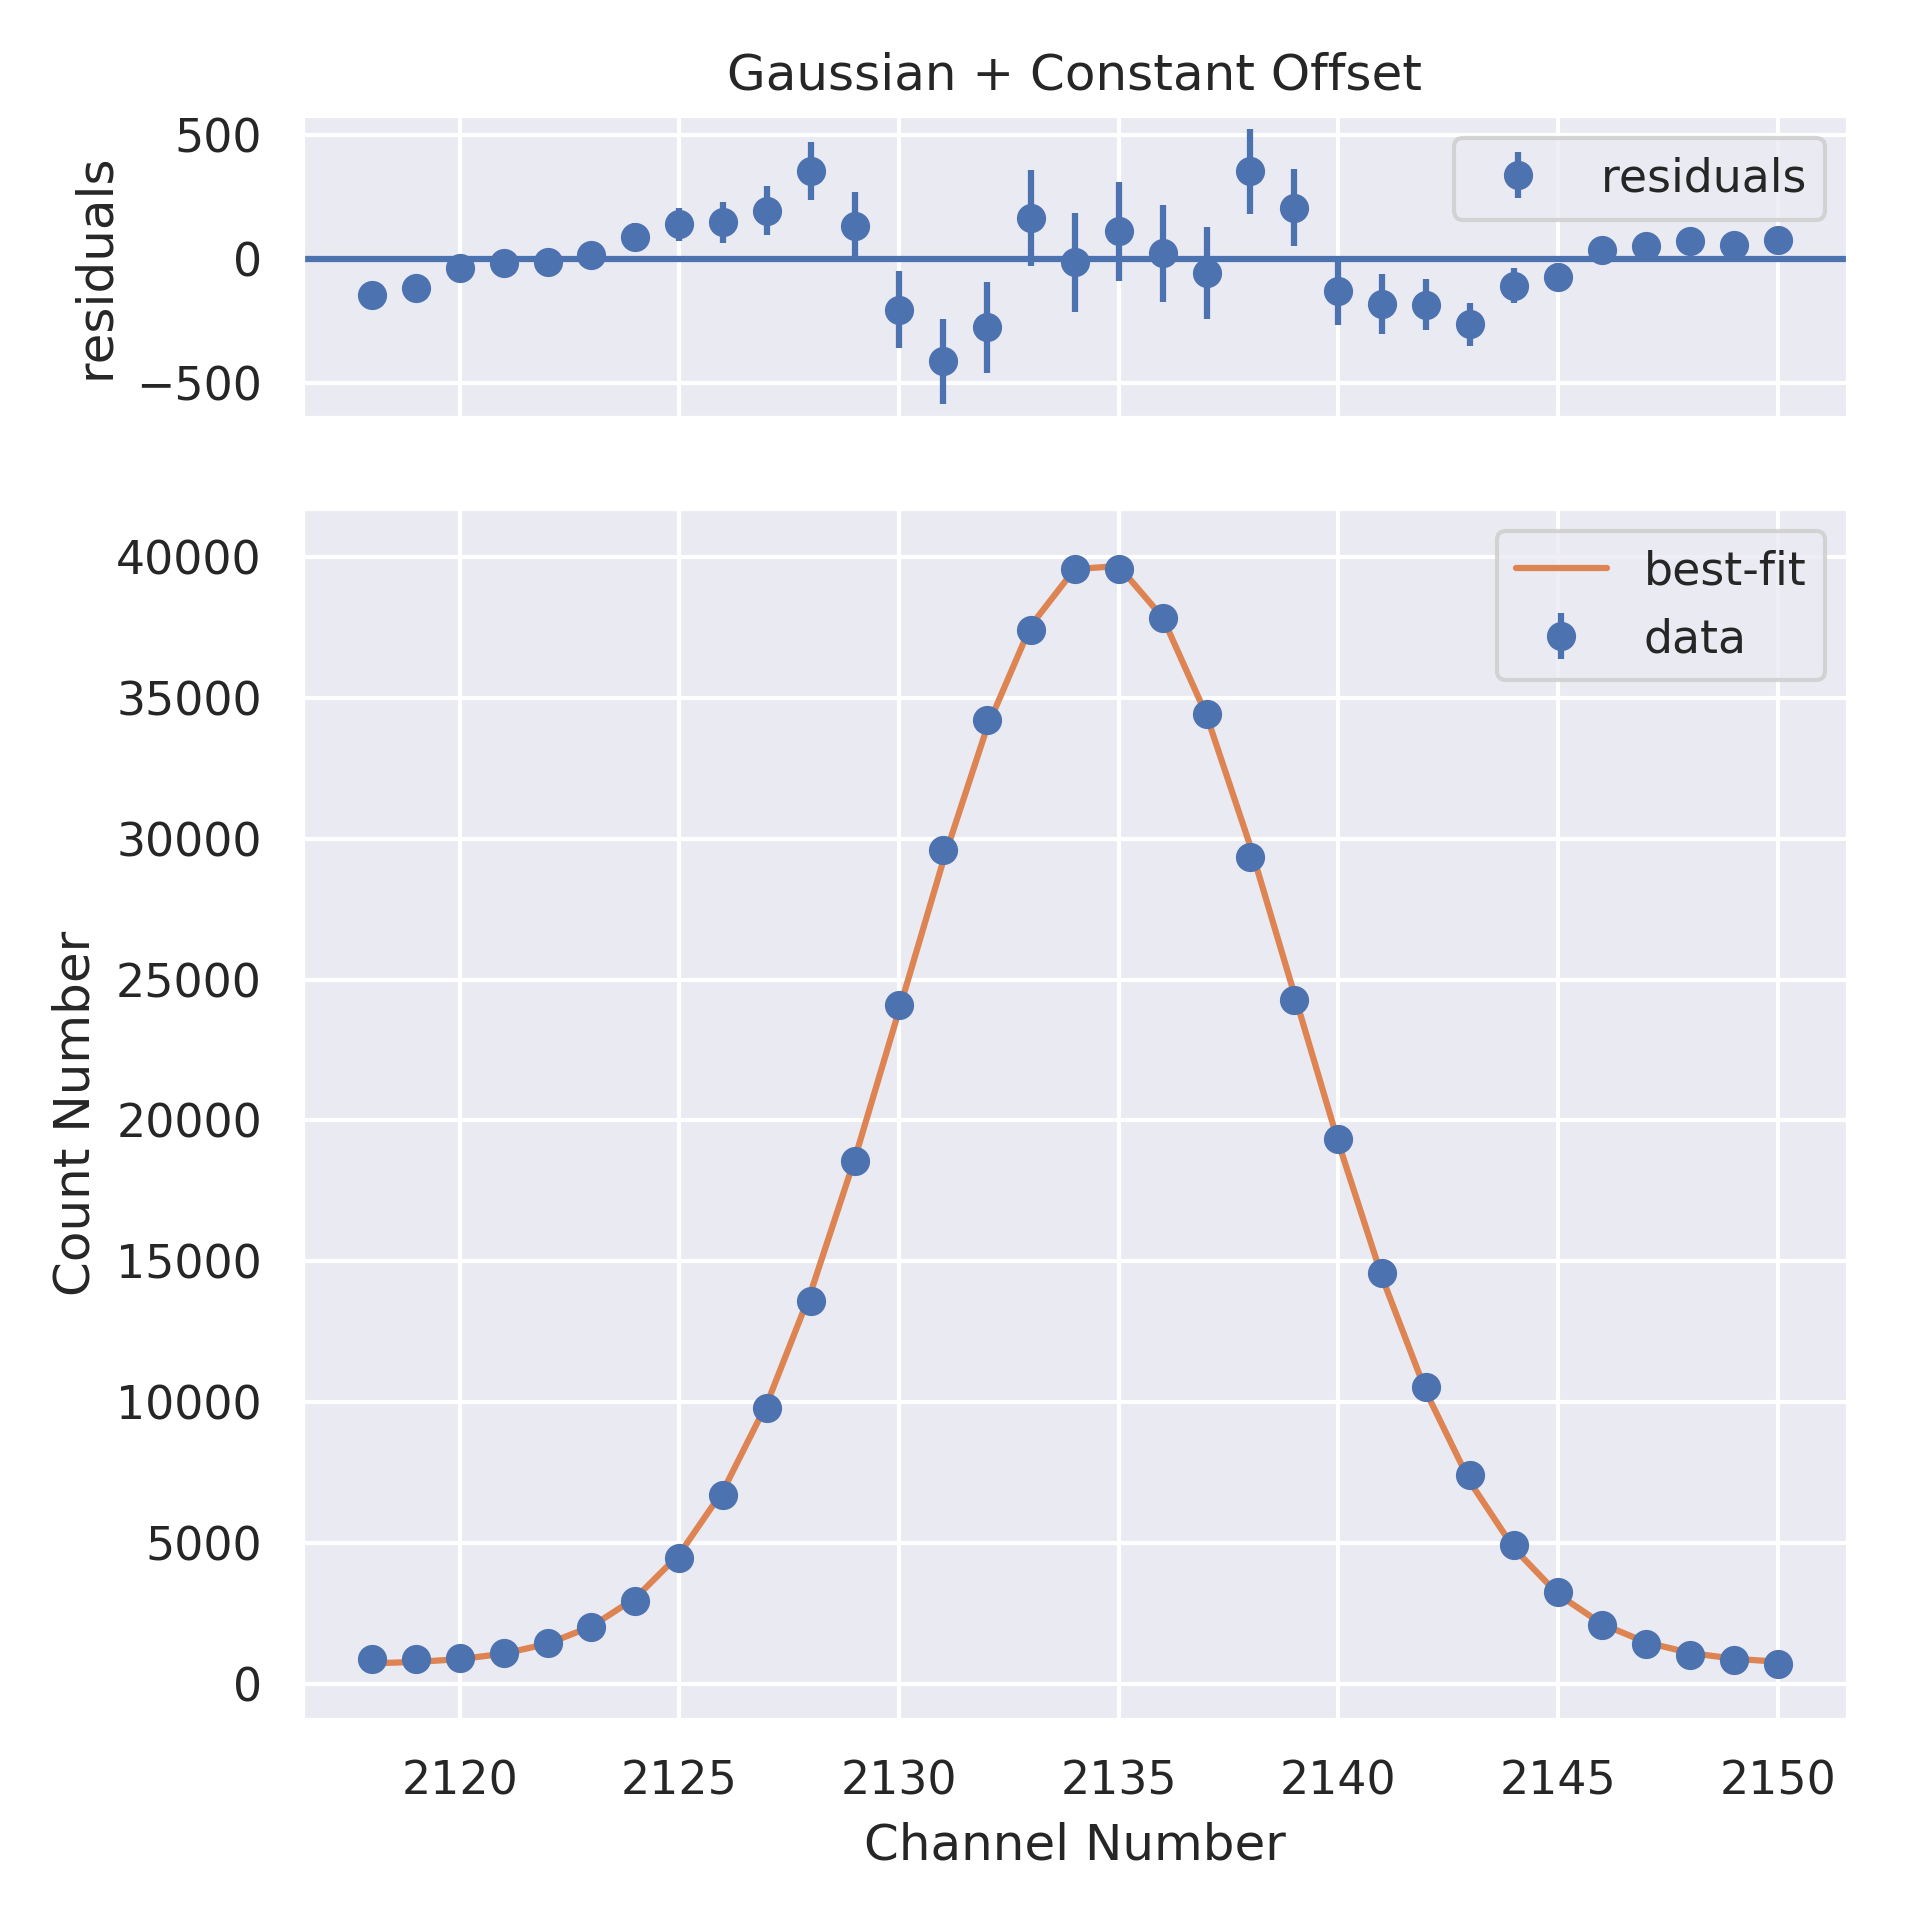
\includegraphics[width=\linewidth]{./Images/Barium133/Gauss/Gauss_5_Full.png}
    \caption{Full peak with fit}
    %\label{fig:sub1}
  \end{subfigure}%
  \begin{subfigure}{.5\linewidth}
    \centering
    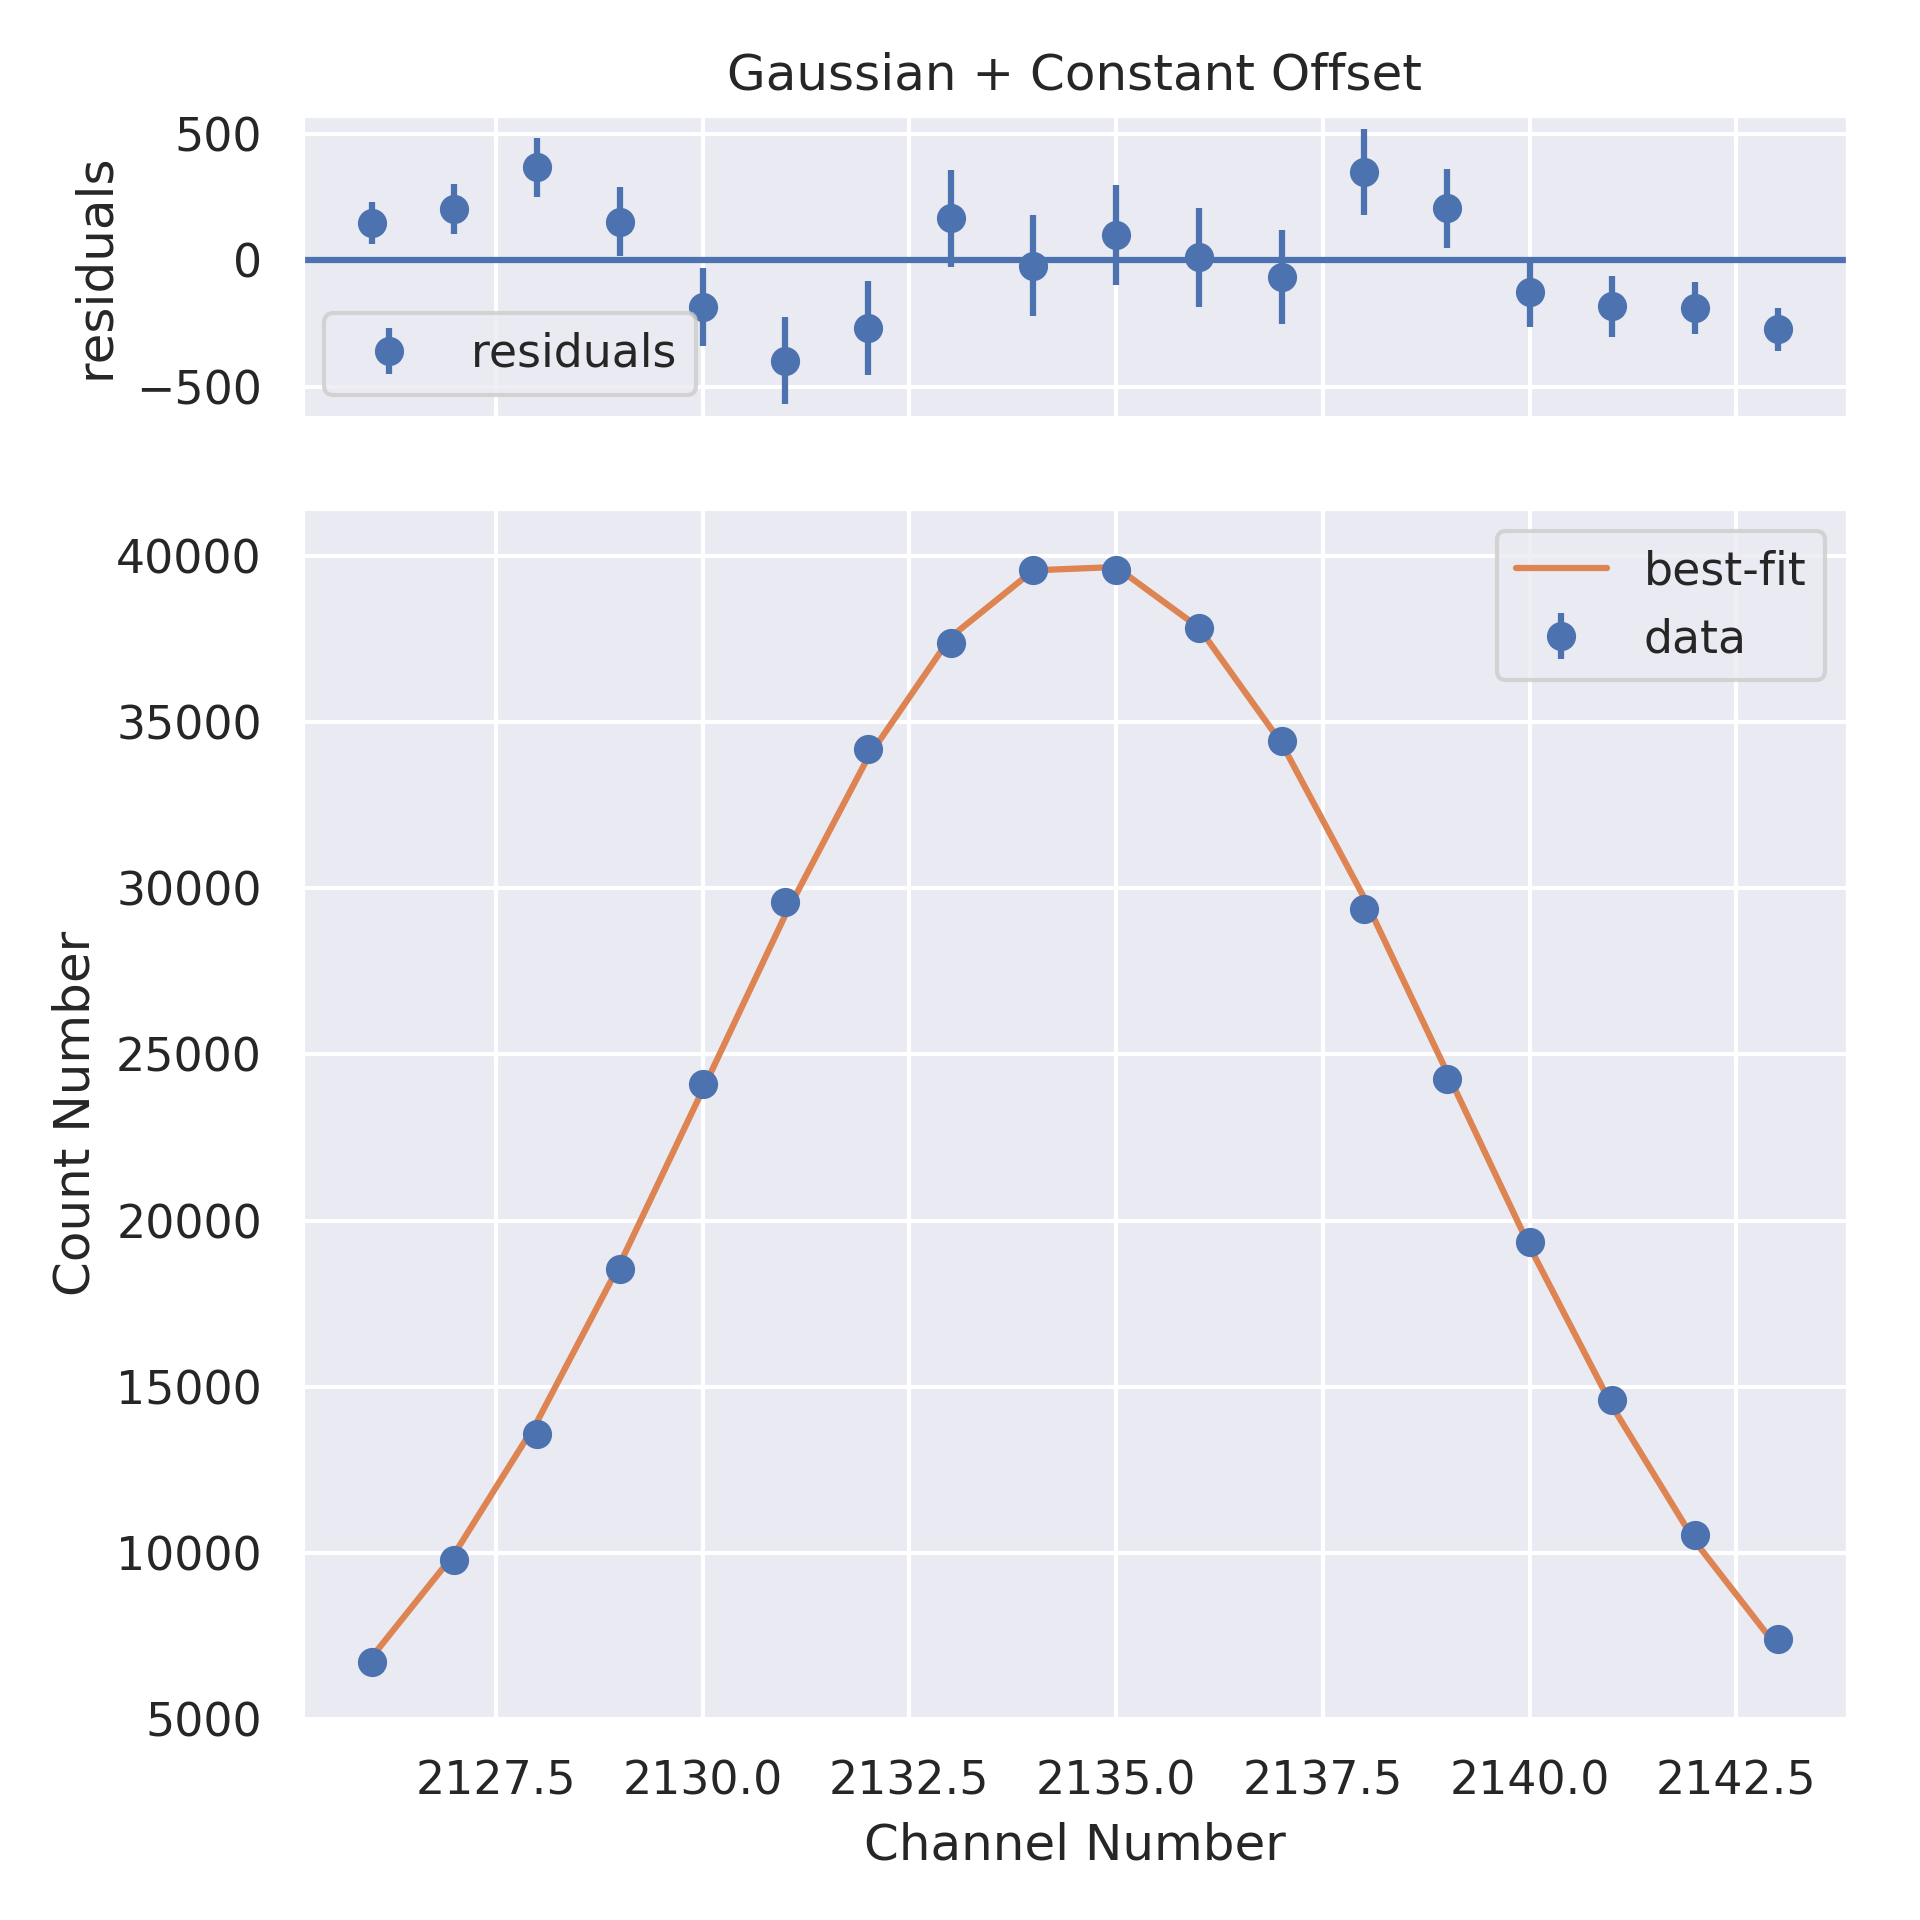
\includegraphics[width=\linewidth]{./Images/Barium133/Gauss/Gauss_5_Zoom.png}
    \caption{Zoomed in peak with fit}
    %\label{fig:sub2}
  \end{subfigure}
  \caption{Fit of full \& zoomed in peak of \element{Ba}{133} 303 keV peak}
  %\label{fig:test}
\end{figure}
\begin{figure}[H]
  \centering
  \begin{subfigure}{.5\linewidth}
    \centering
    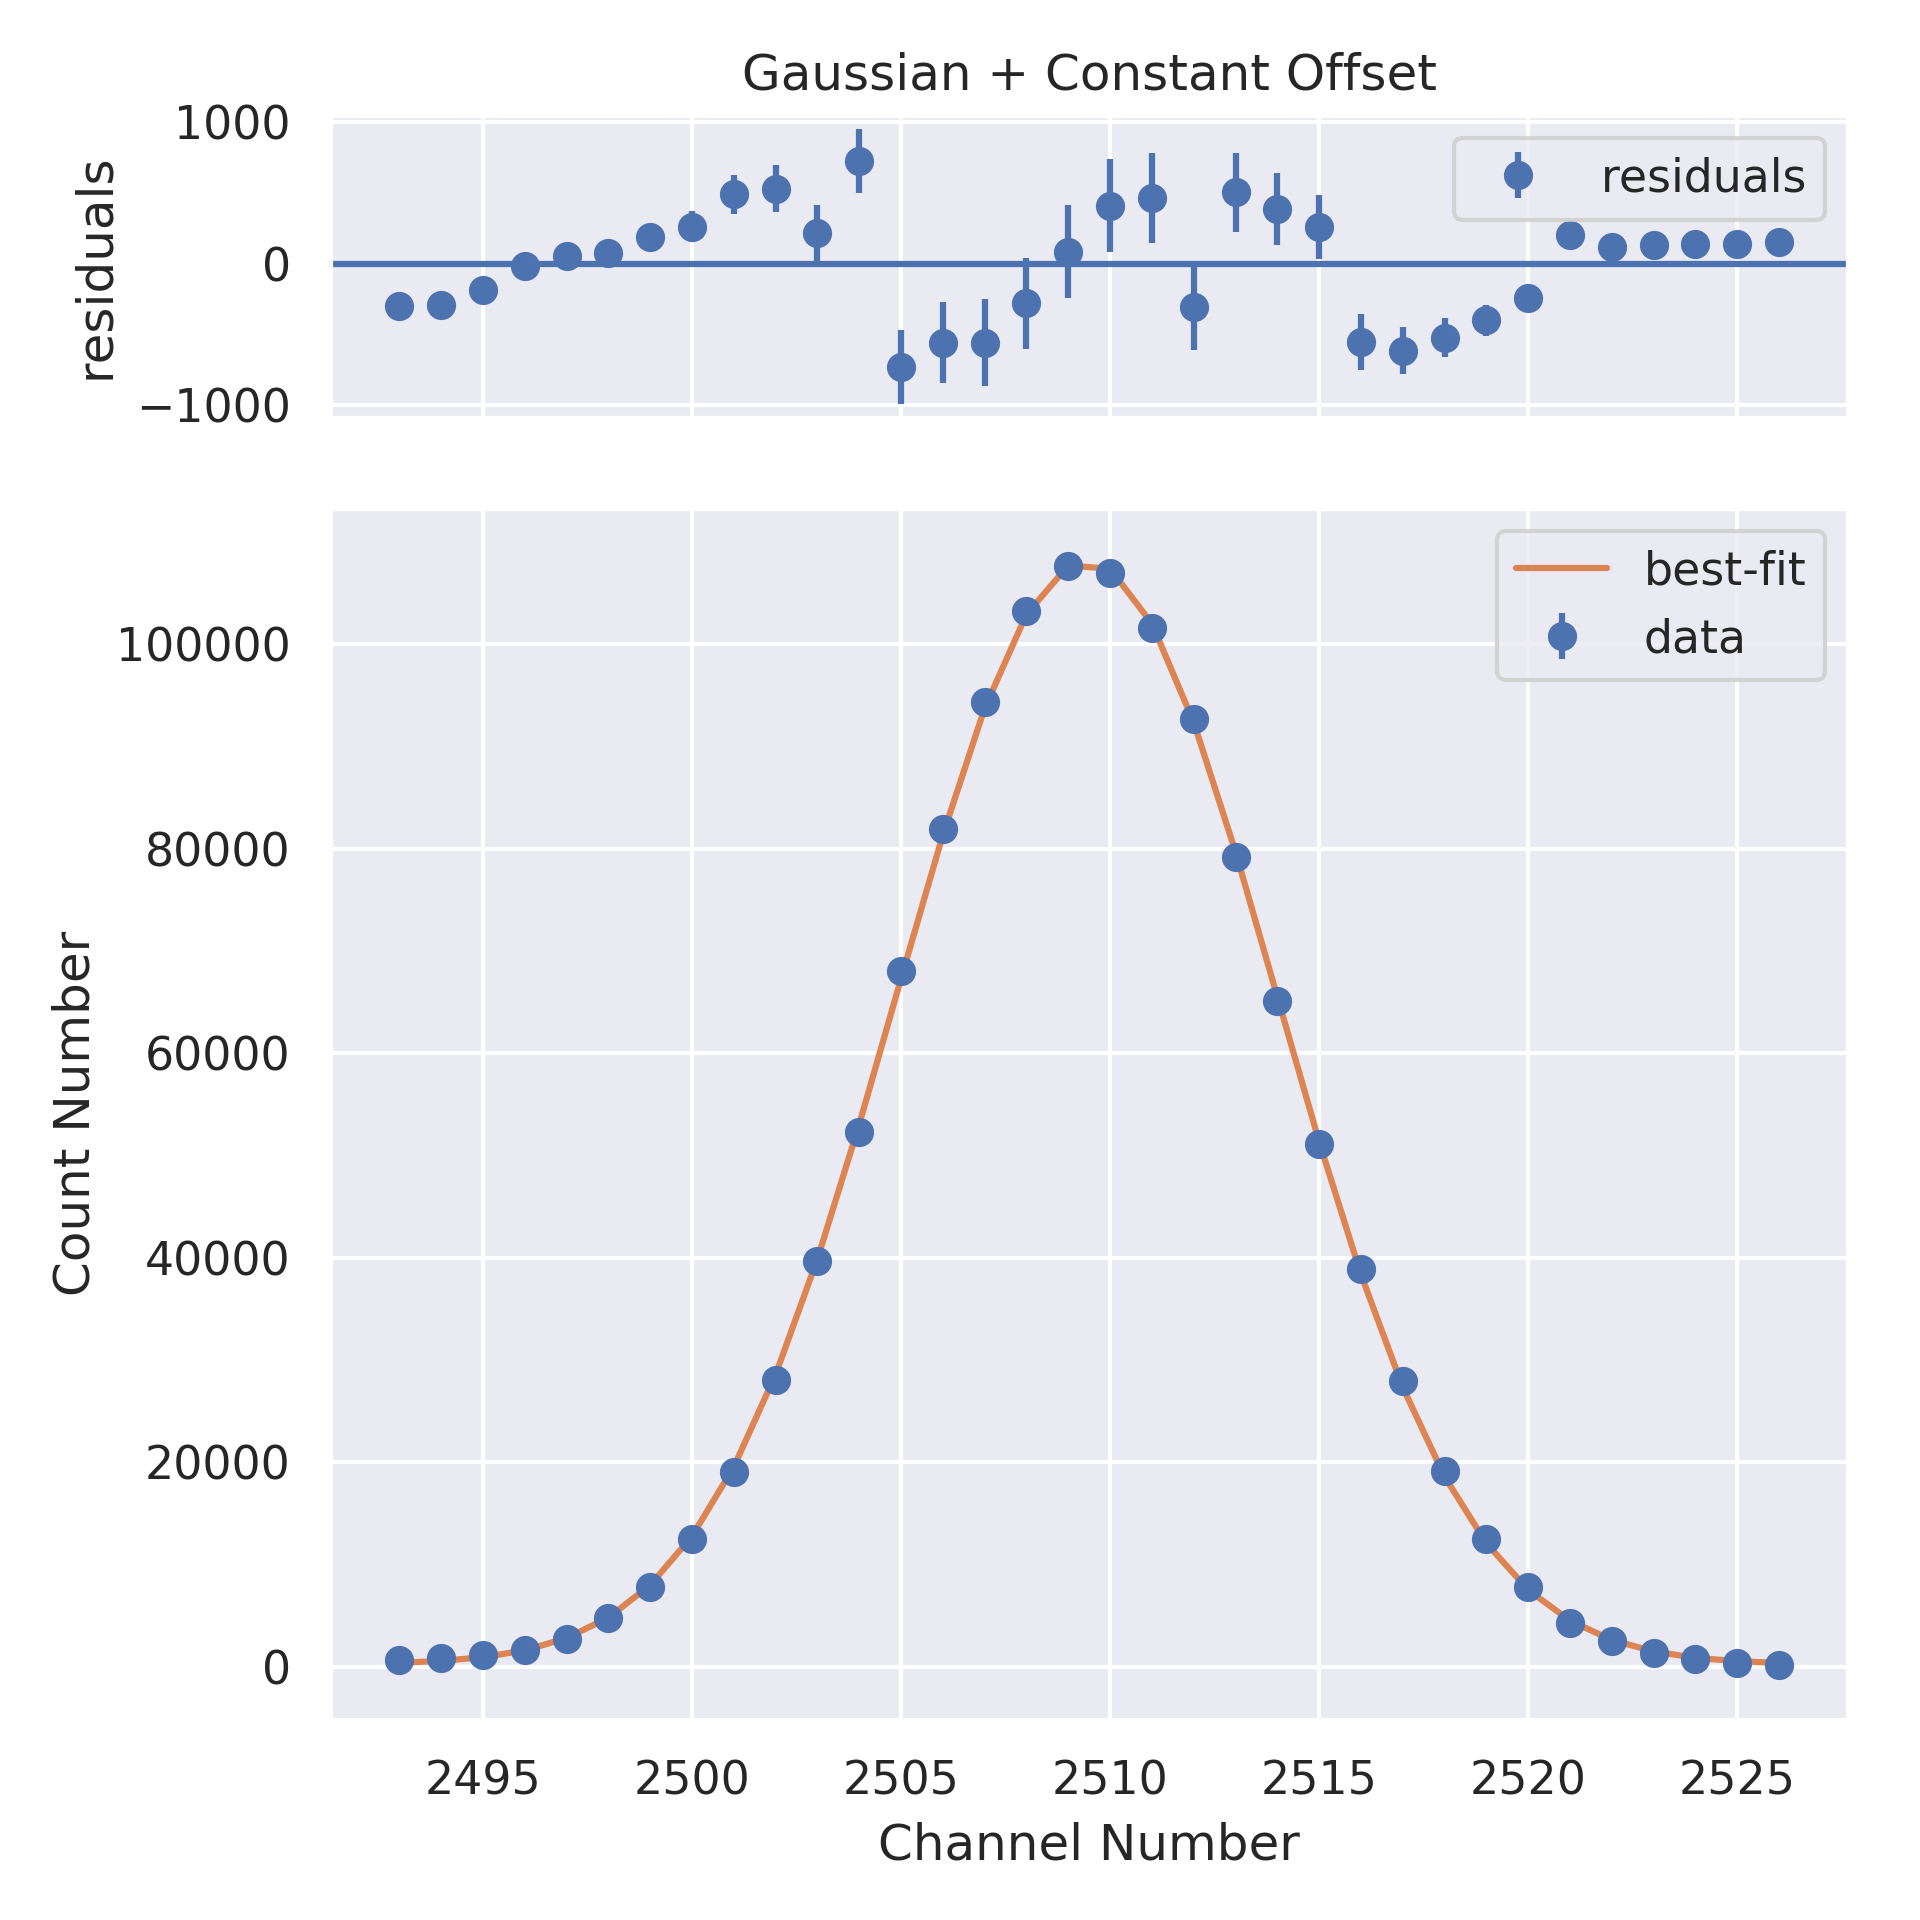
\includegraphics[width=\linewidth]{./Images/Barium133/Gauss/Gauss_6_Full.png}
    \caption{Full peak with fit}
    %\label{fig:sub1}
  \end{subfigure}%
  \begin{subfigure}{.5\linewidth}
    \centering
    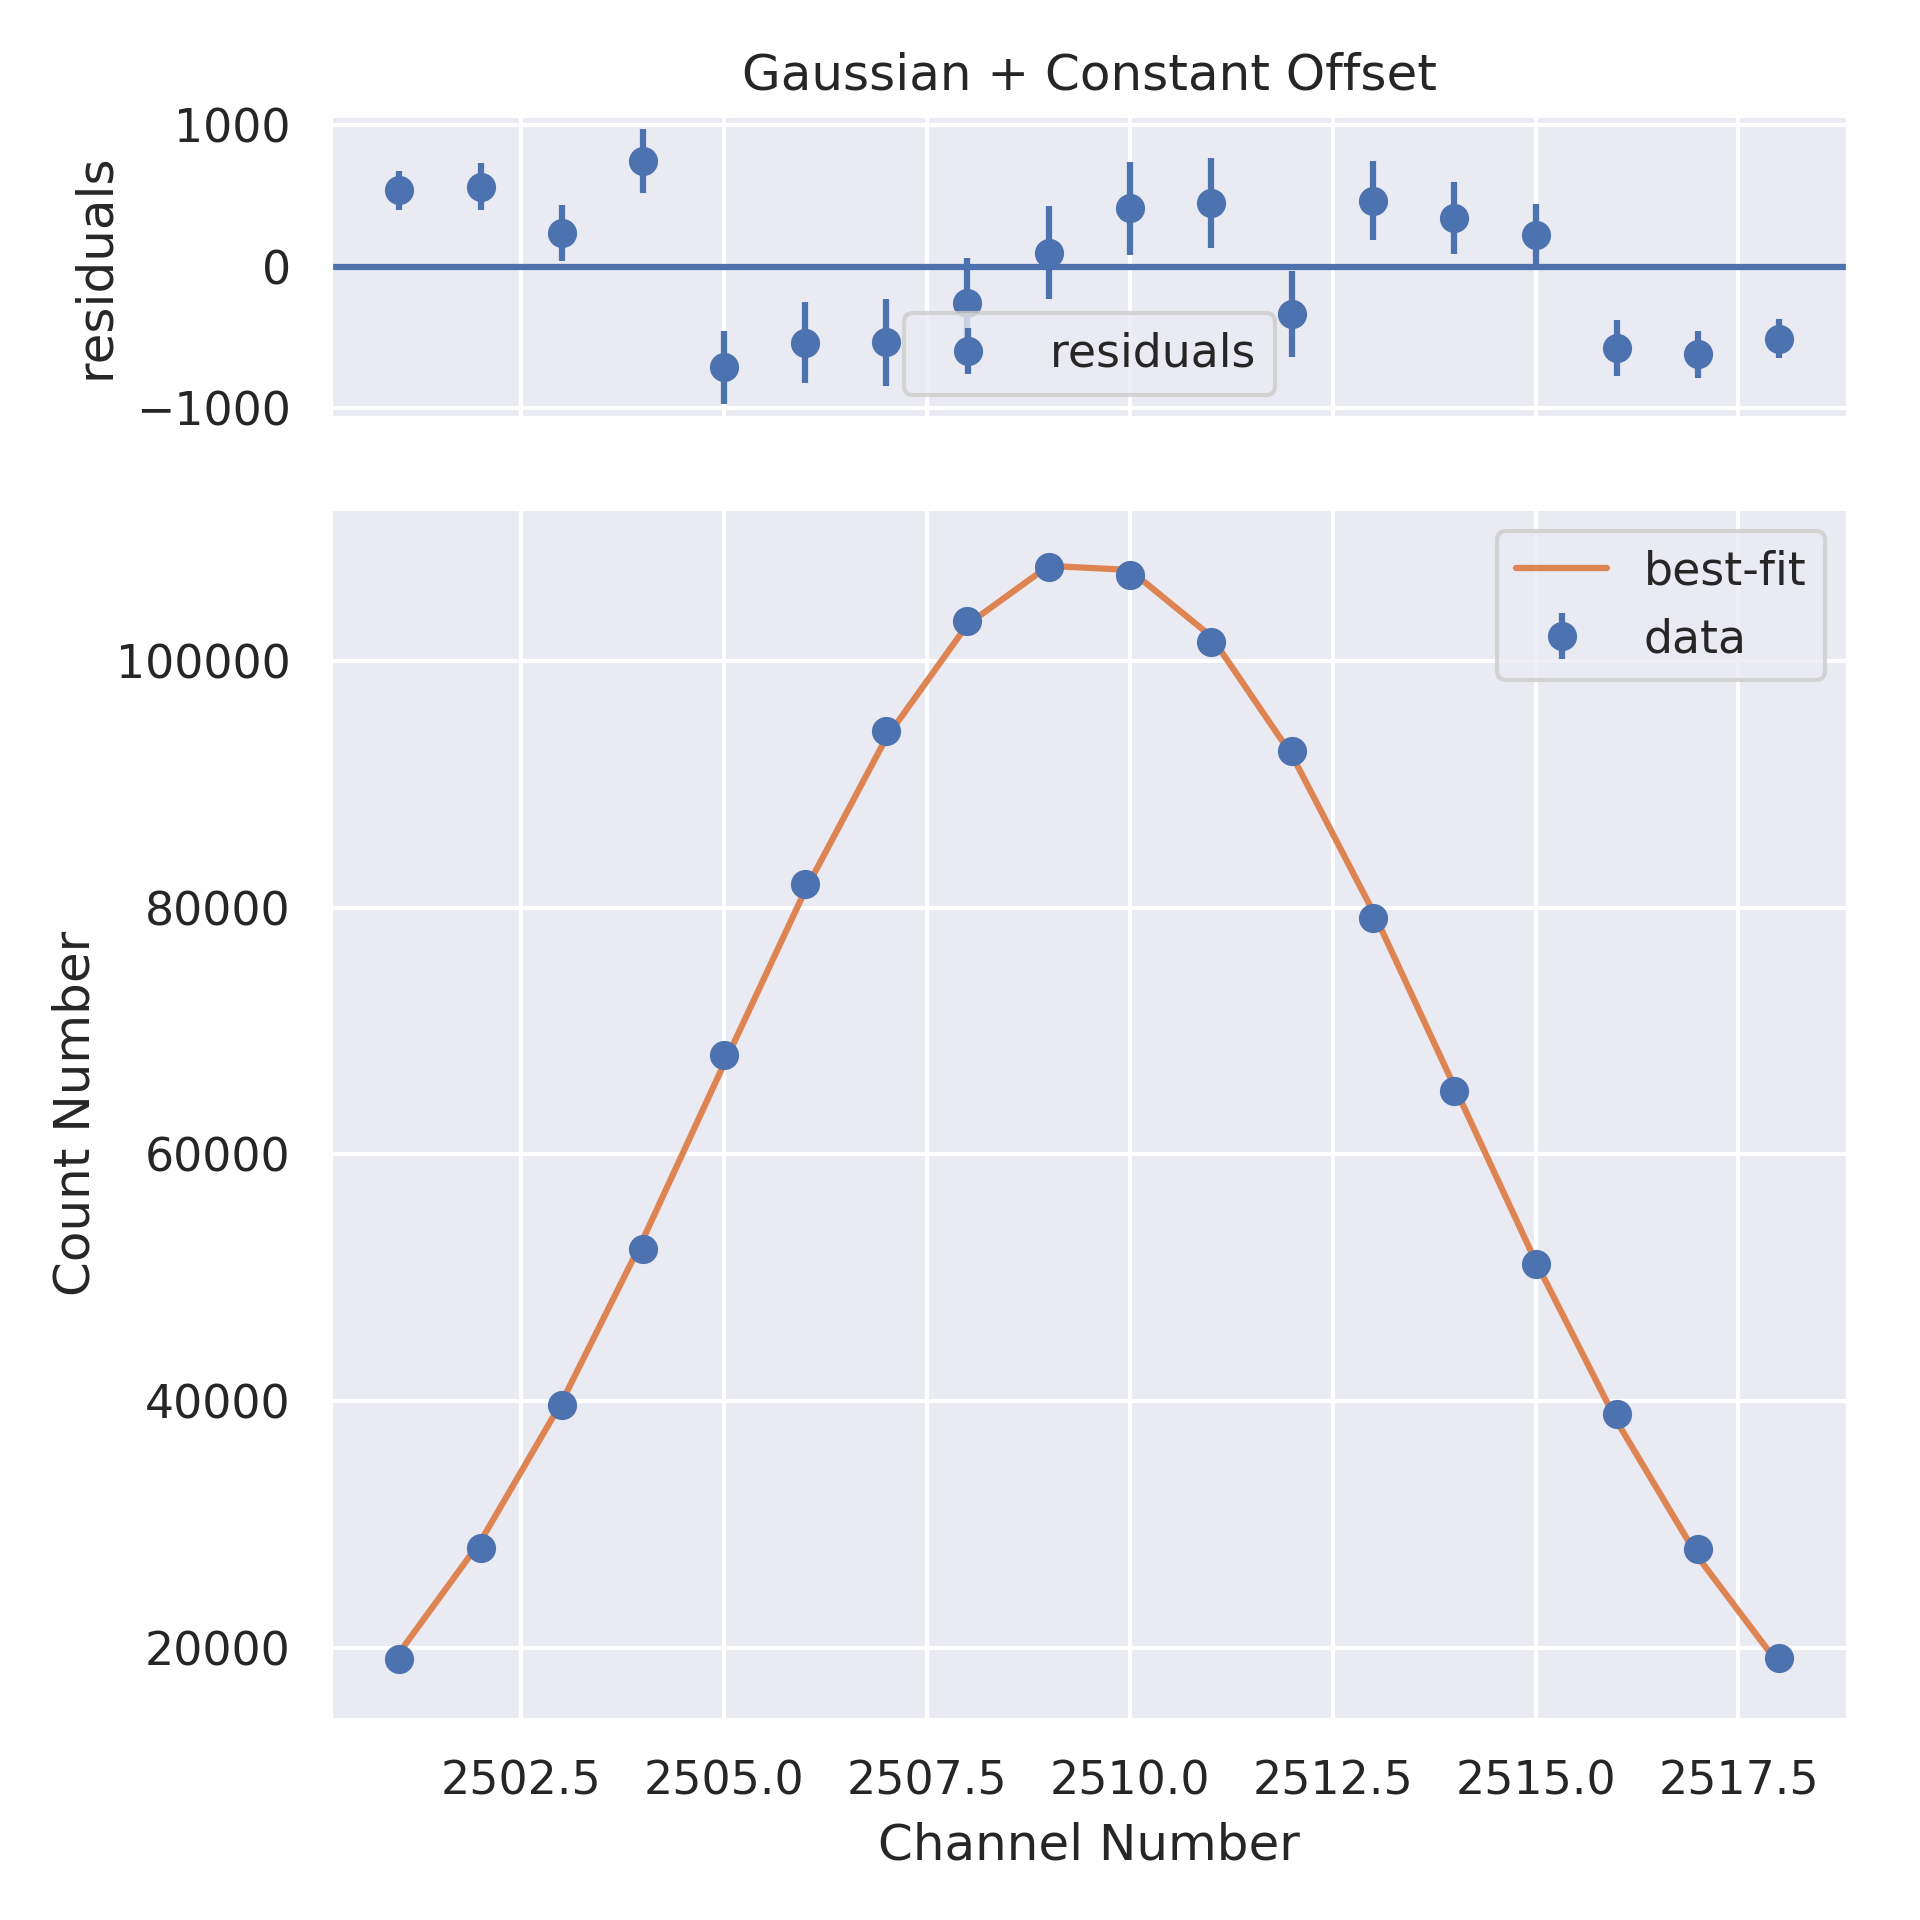
\includegraphics[width=\linewidth]{./Images/Barium133/Gauss/Gauss_6_Zoom.png}
    \caption{Zoomed in peak with fit}
    %\label{fig:sub2}
  \end{subfigure}
  \caption{Fit of full \& zoomed in peak of \element{Ba}{133} 356 keV peak}
  %\label{fig:test}
\end{figure}
\begin{figure}[H]
  \centering
  \begin{subfigure}{.5\linewidth}
    \centering
    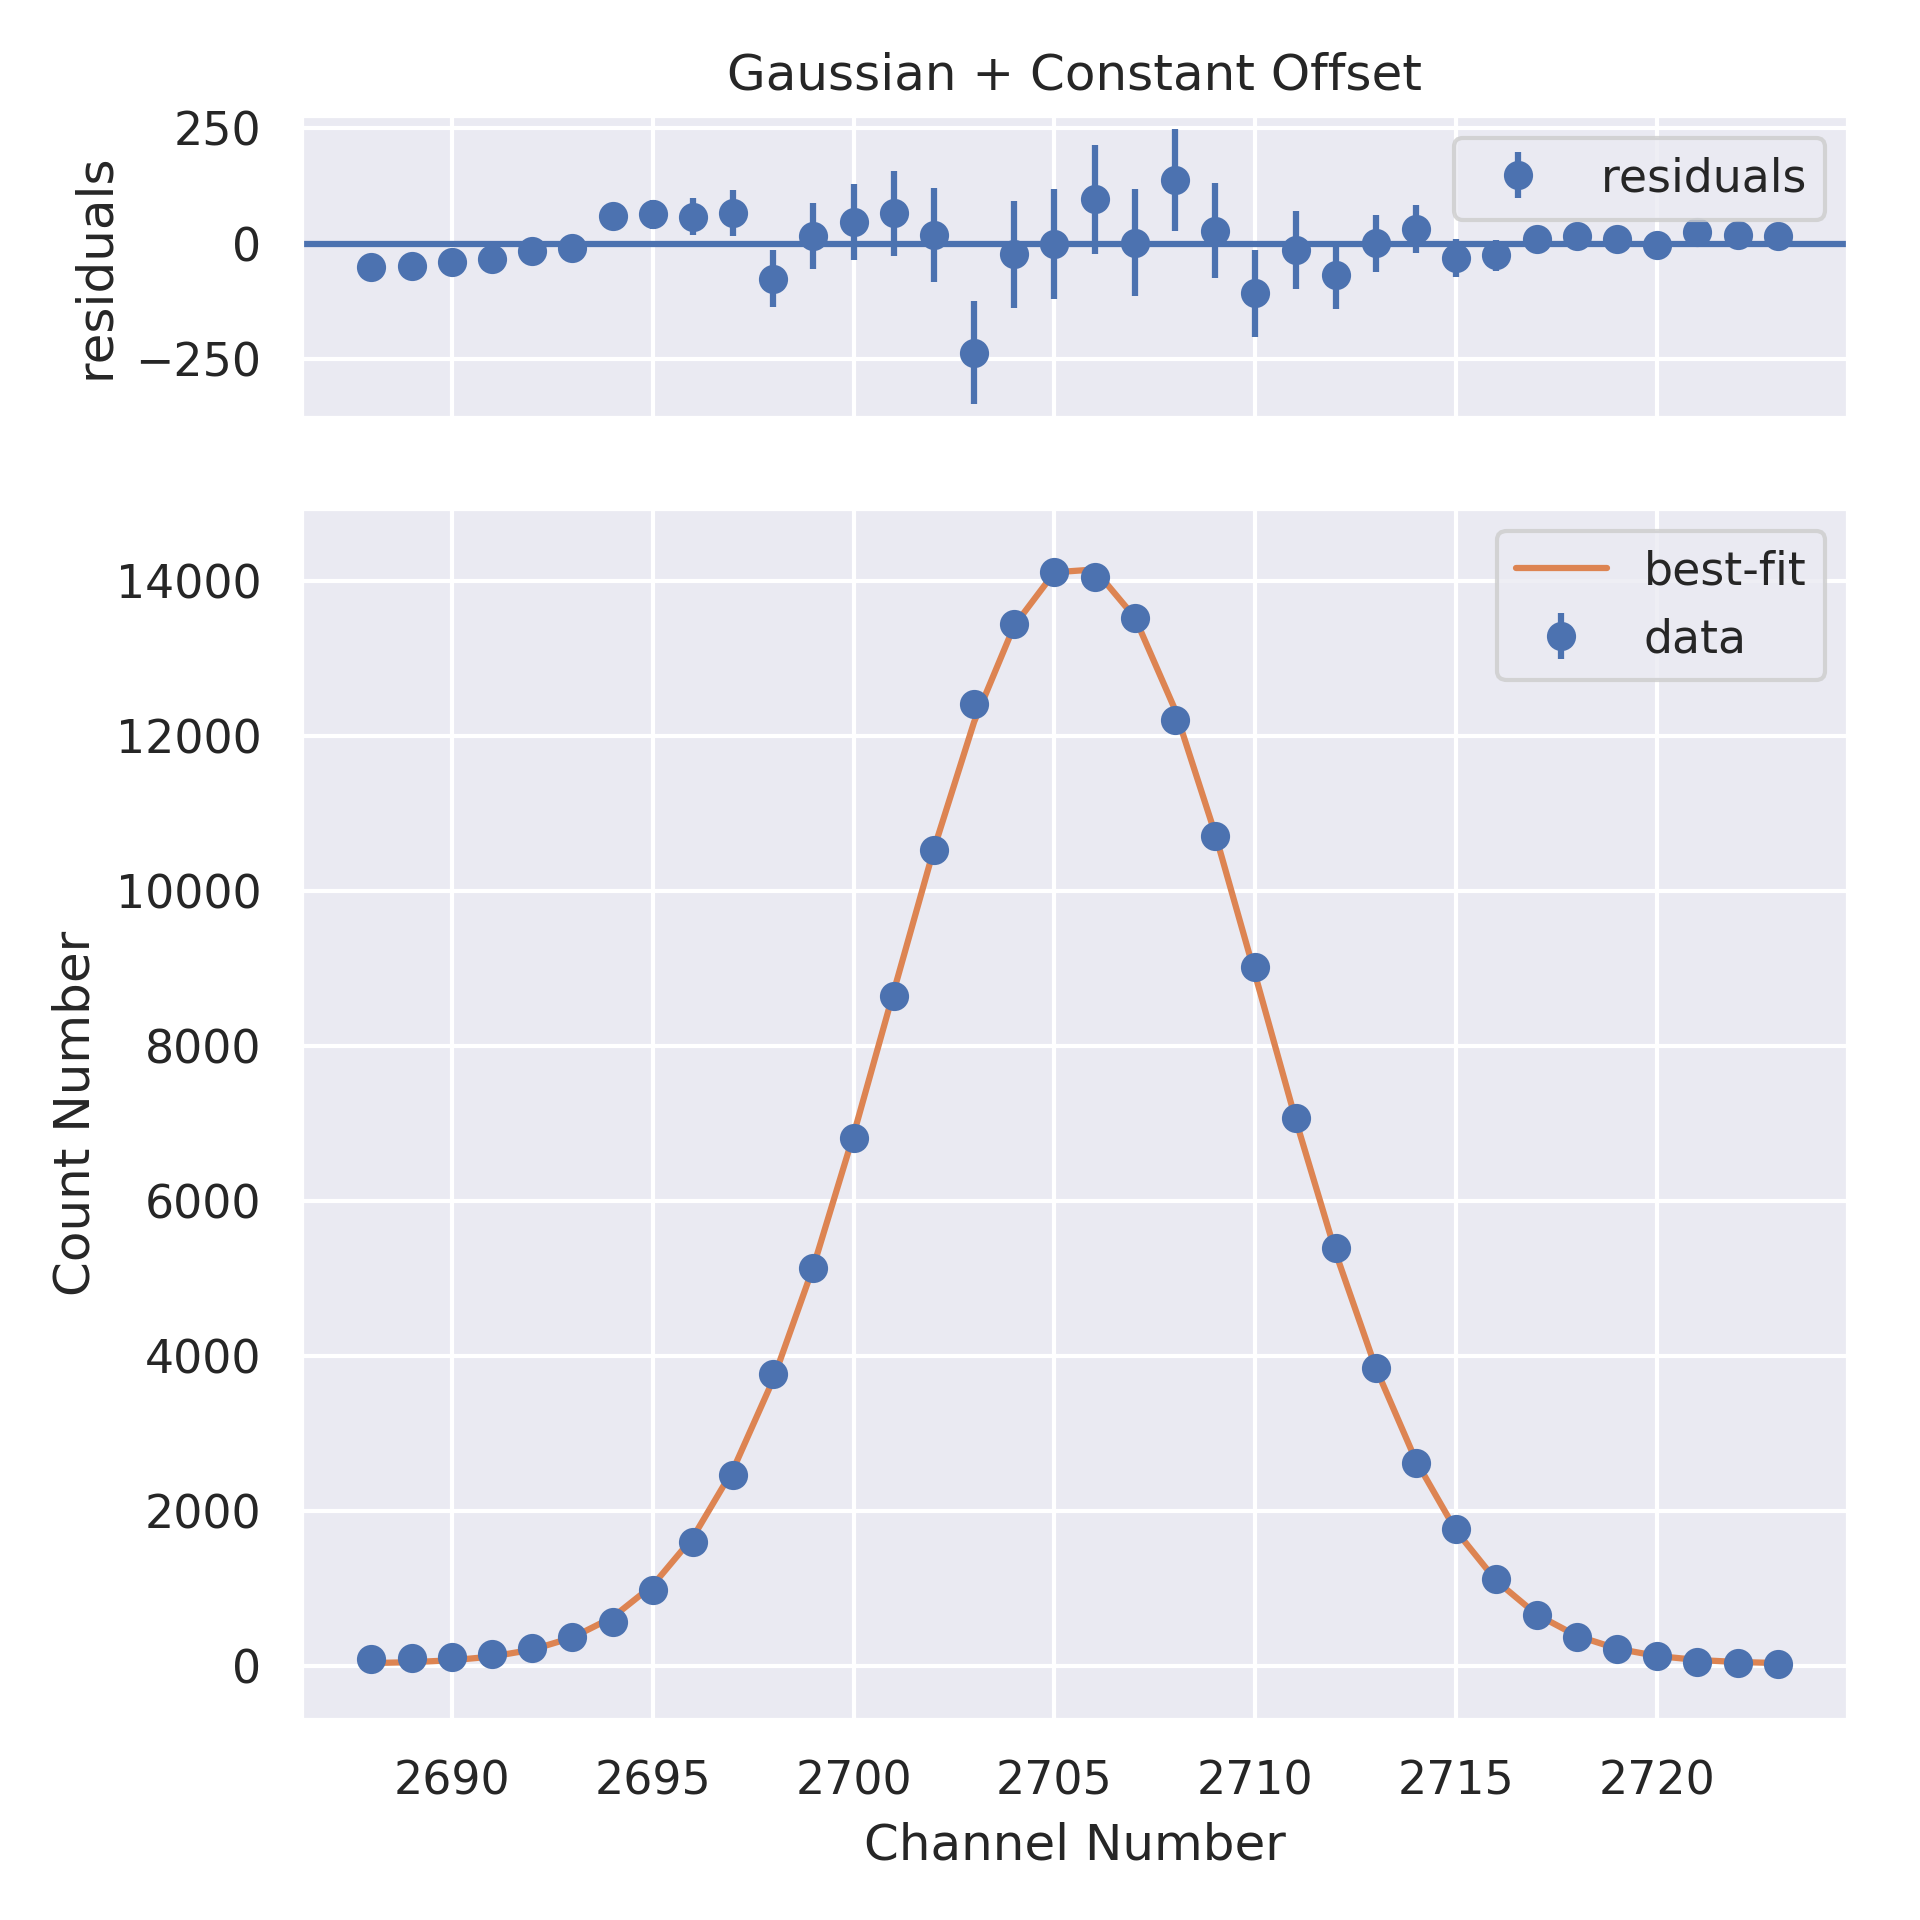
\includegraphics[width=\linewidth]{./Images/Barium133/Gauss/Gauss_7_Full.png}
    \caption{Full peak with fit}
    %\label{fig:sub1}
  \end{subfigure}%
  \begin{subfigure}{.5\linewidth}
    \centering
    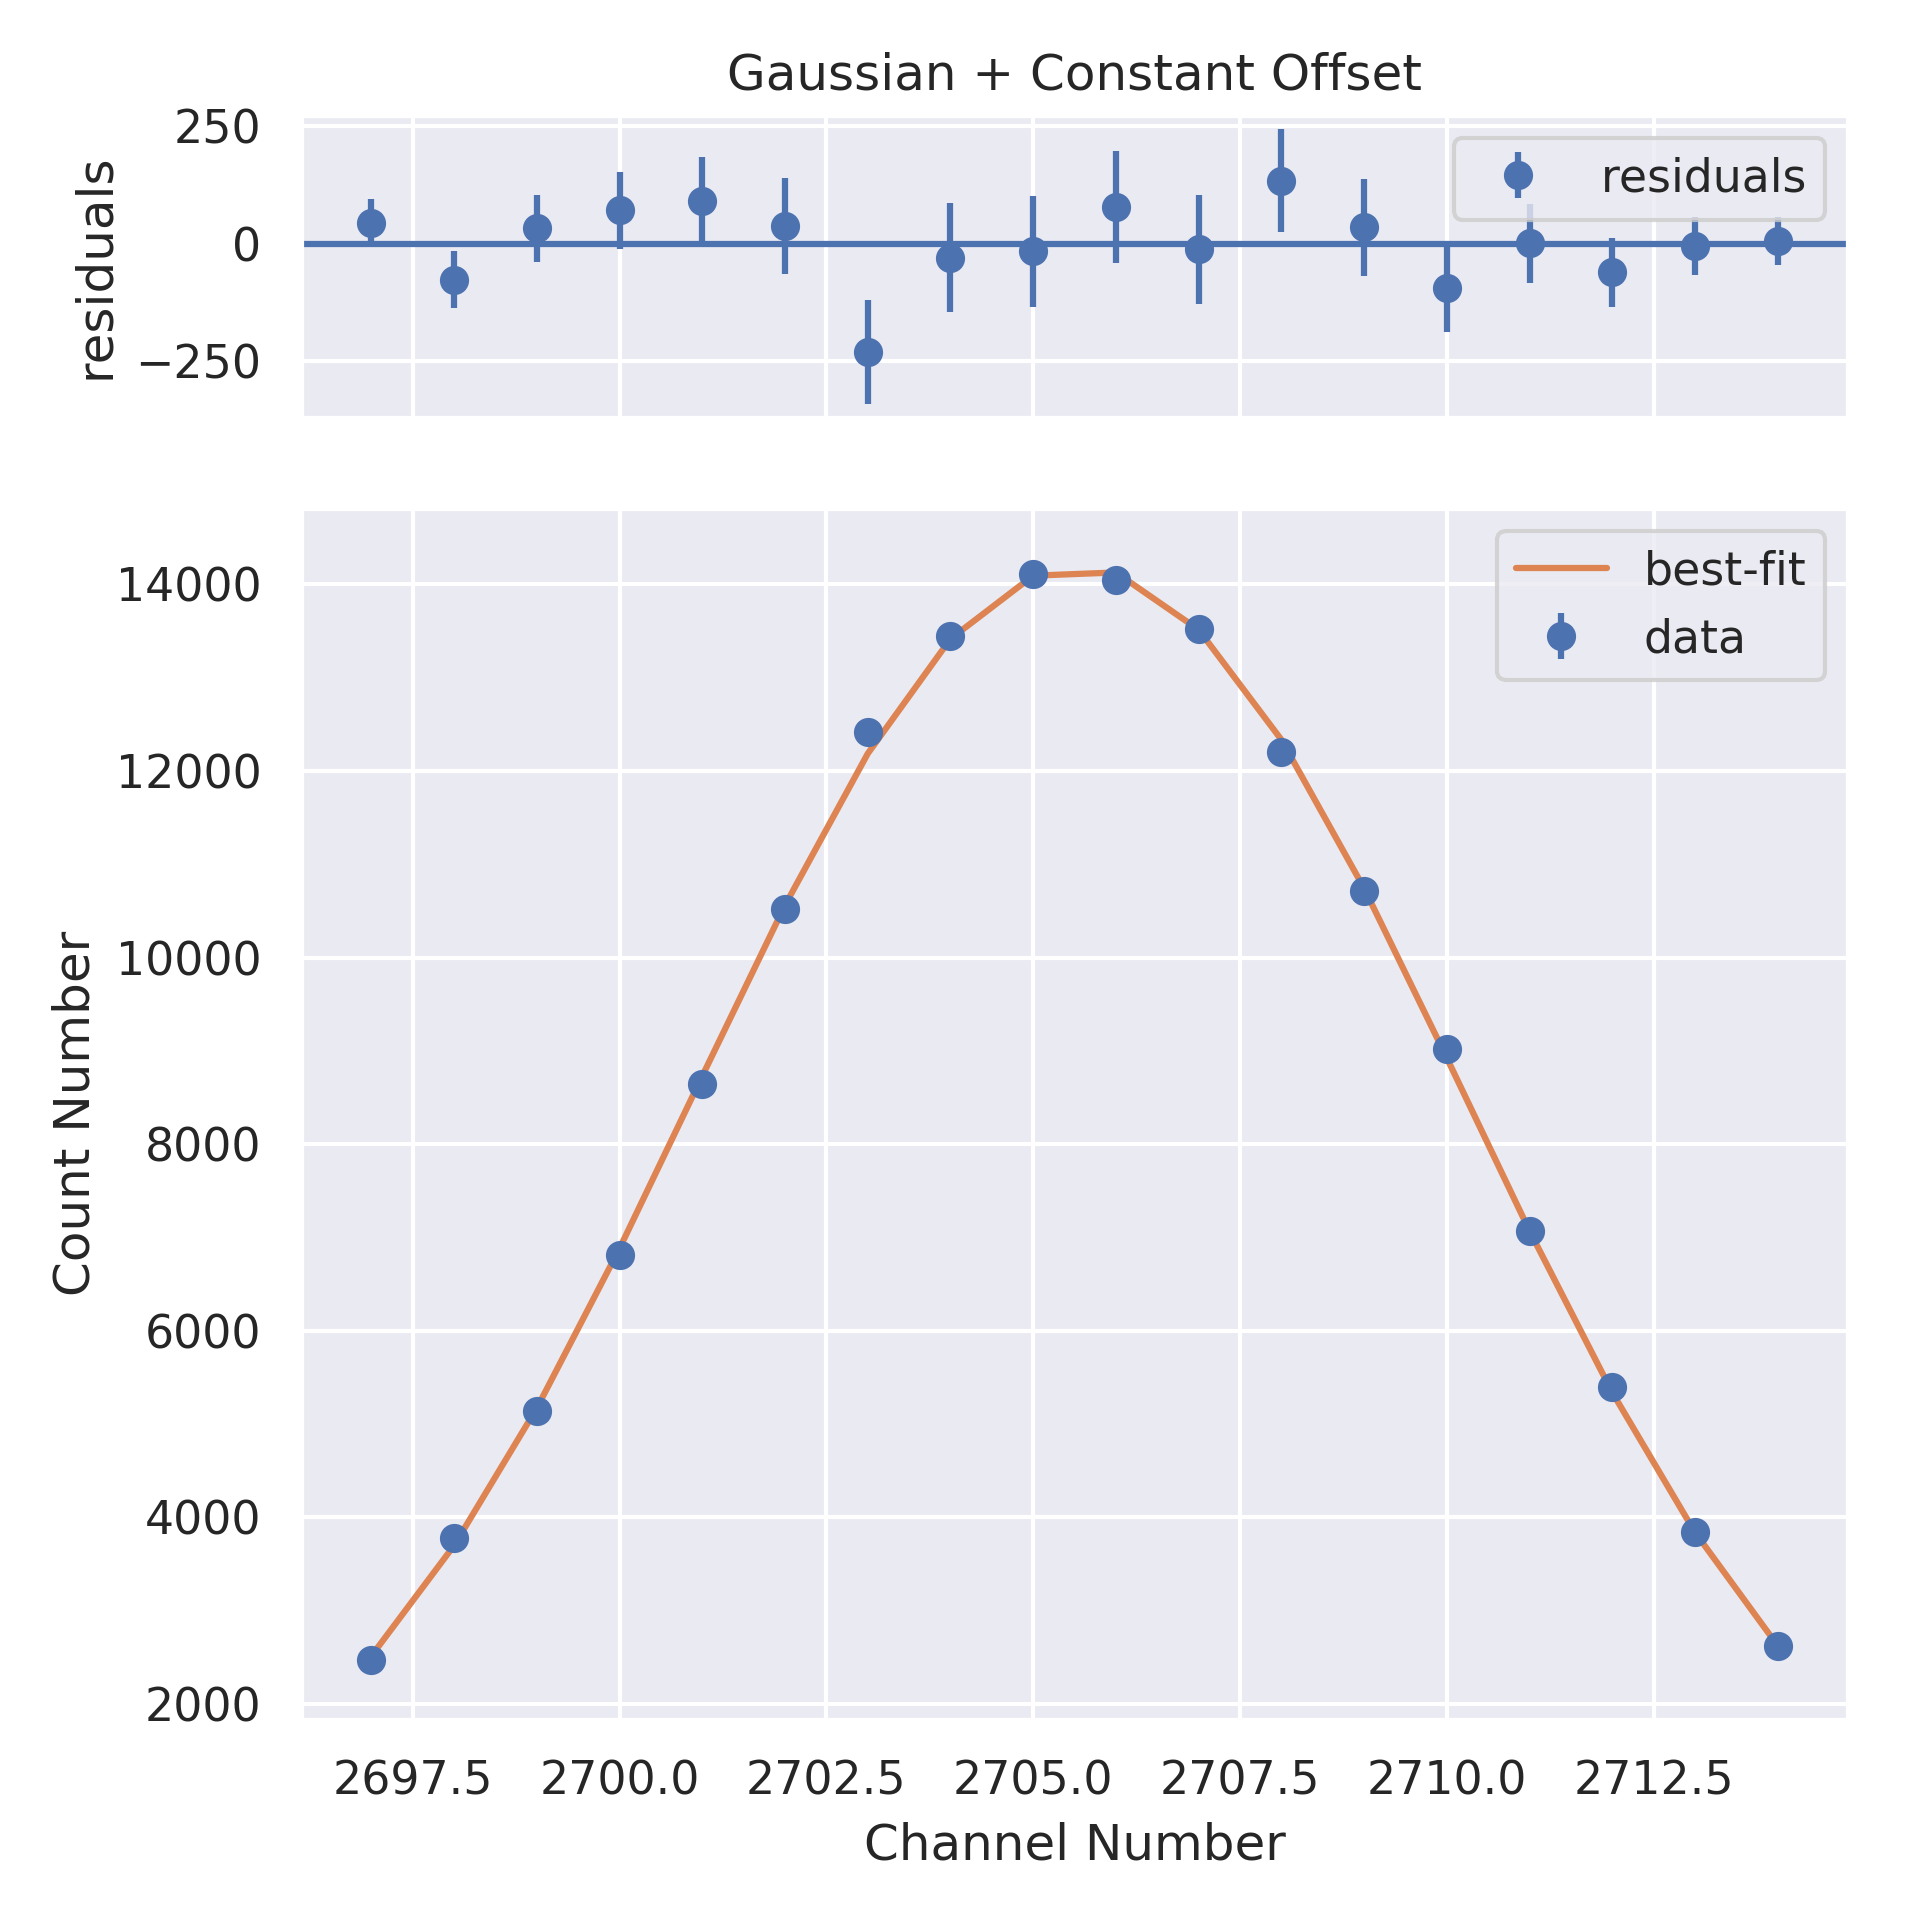
\includegraphics[width=\linewidth]{./Images/Barium133/Gauss/Gauss_7_Zoom.png}
    \caption{Zoomed in peak with fit}
    %\label{fig:sub2}
  \end{subfigure}
  \caption{Fit of full \& zoomed in peak of \element{Ba}{133} 384 keV peak}
  %\label{fig:test}
\end{figure}
\clearpage
\subsubsection{Linear + Gaussian Fit}
\begin{figure}[H]
  \centering
  \begin{subfigure}{.5\linewidth}
    \centering
    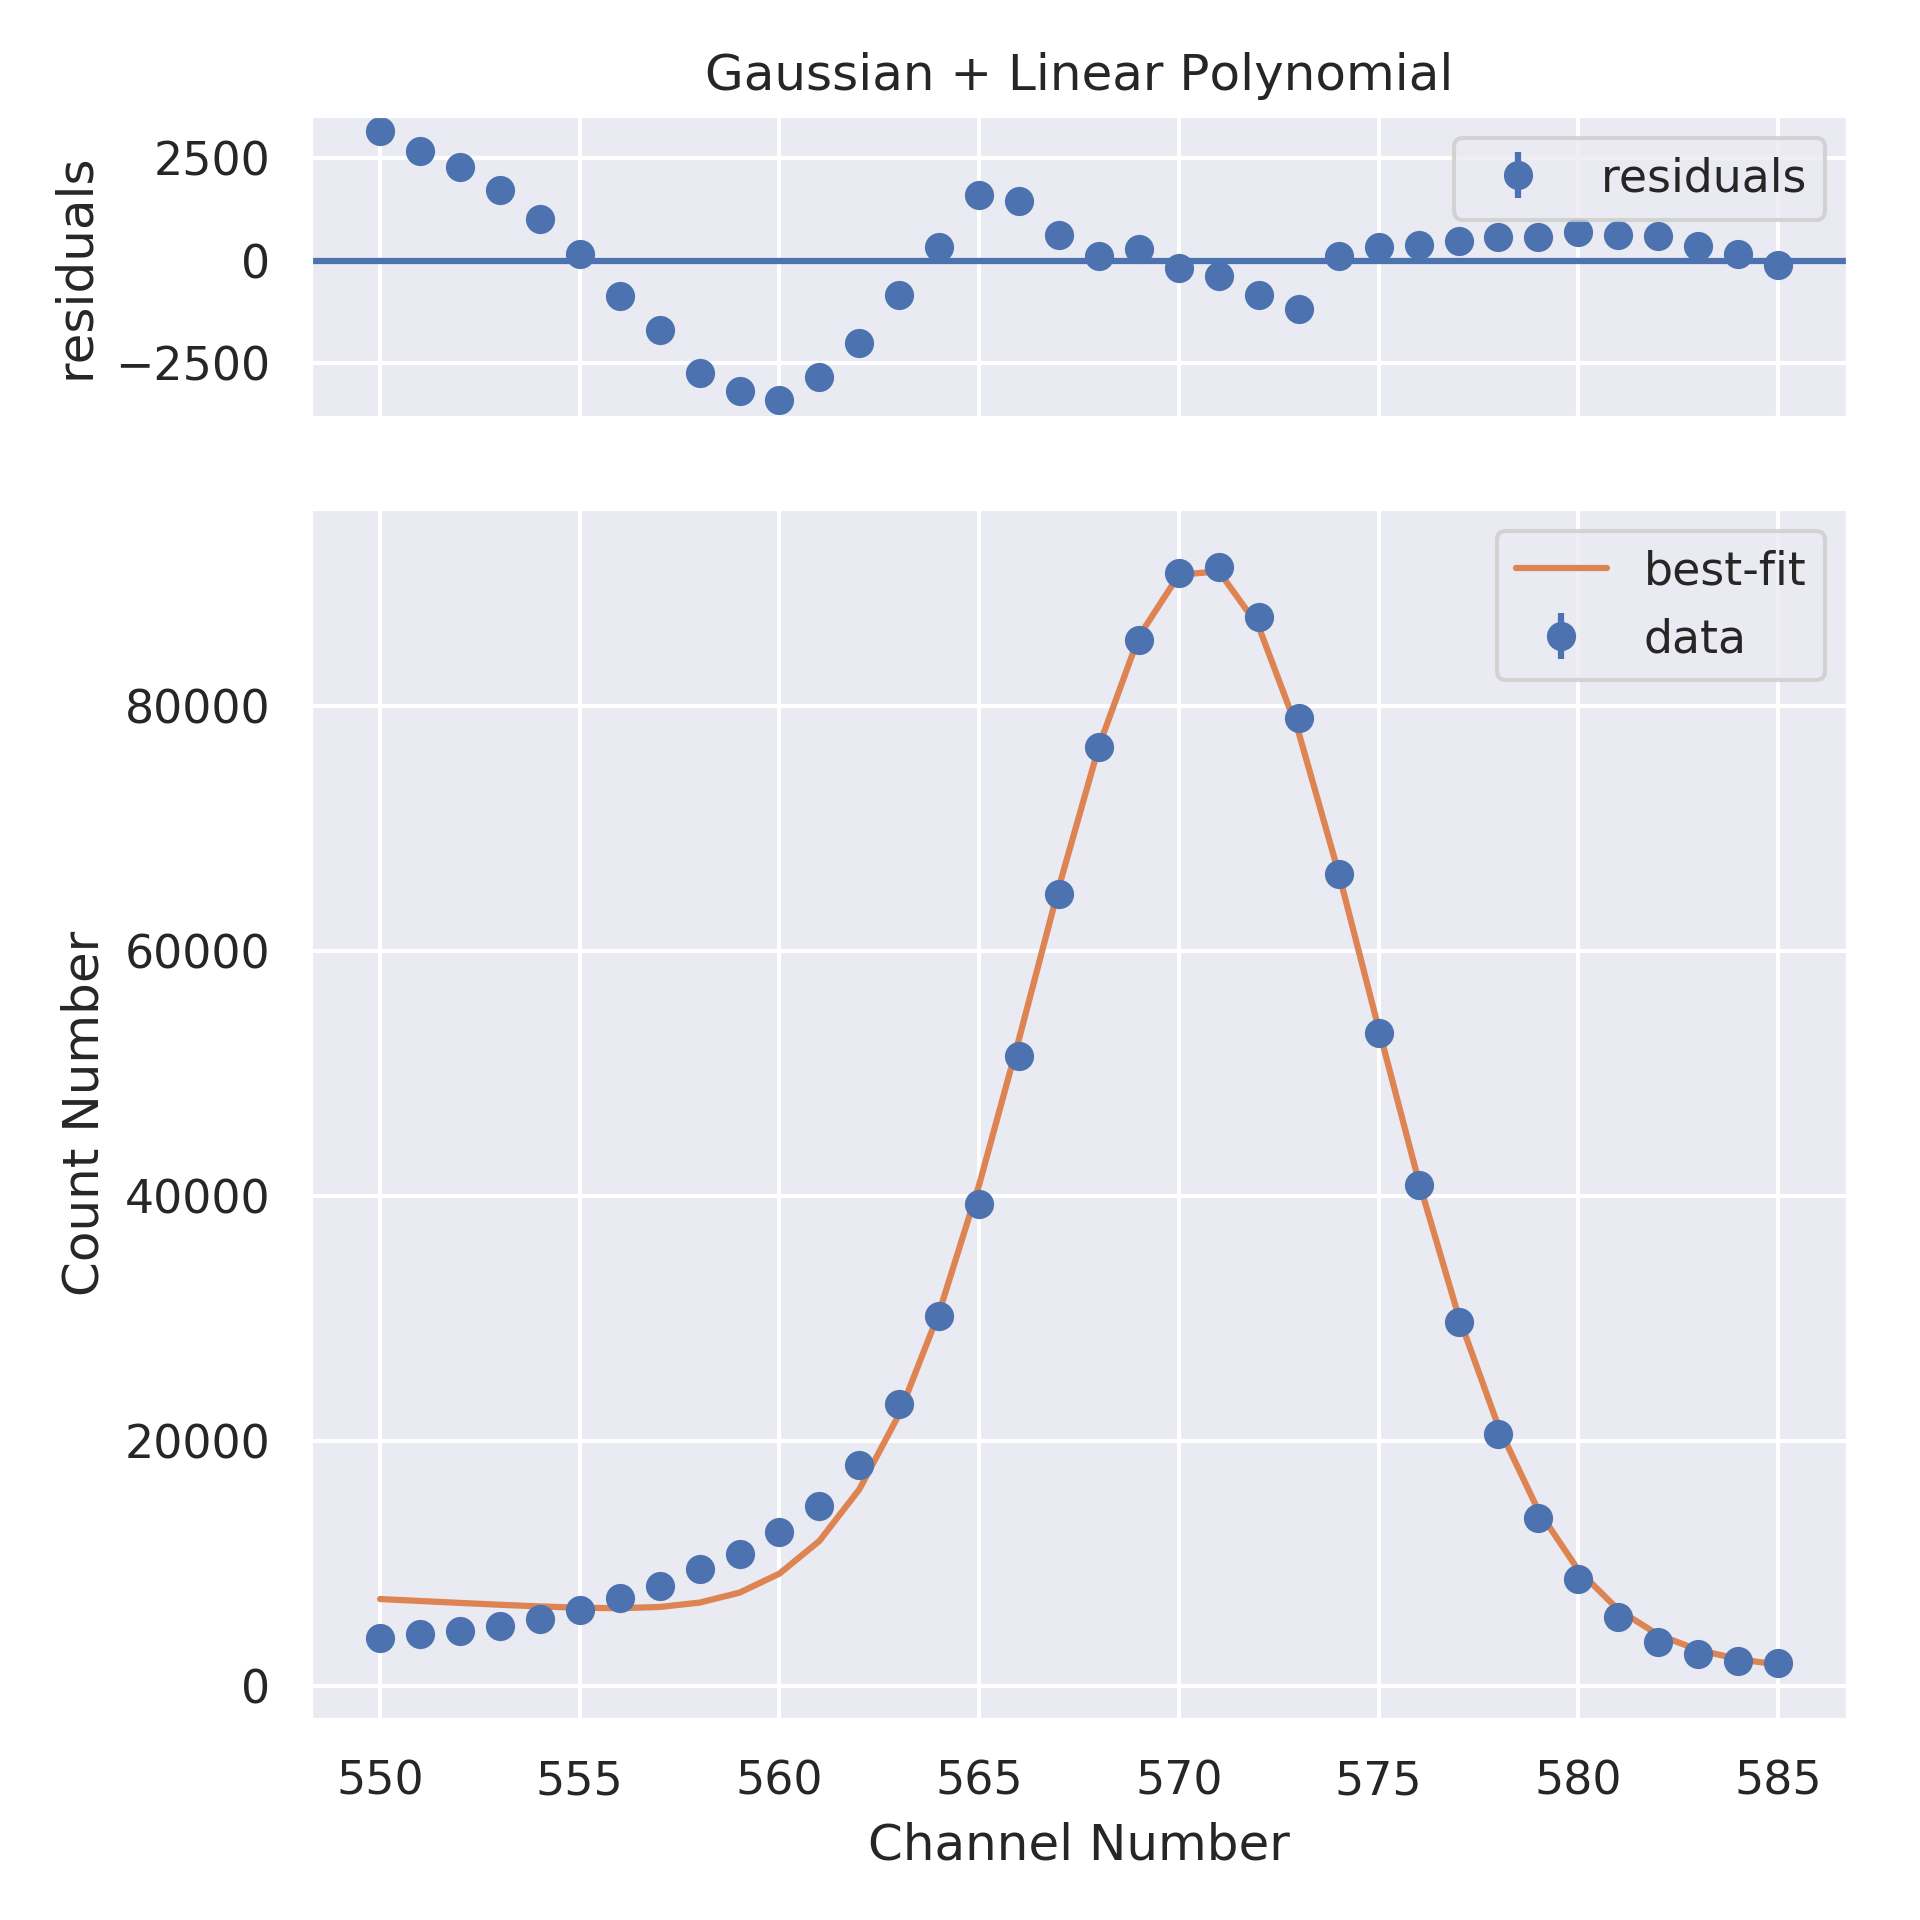
\includegraphics[width=\linewidth]{./Images/Barium133/Linear/Linear_1_Full.png}
    \caption{Full peak with fit}
    %\label{fig:sub1}
  \end{subfigure}%
  \begin{subfigure}{.5\linewidth}
    \centering
    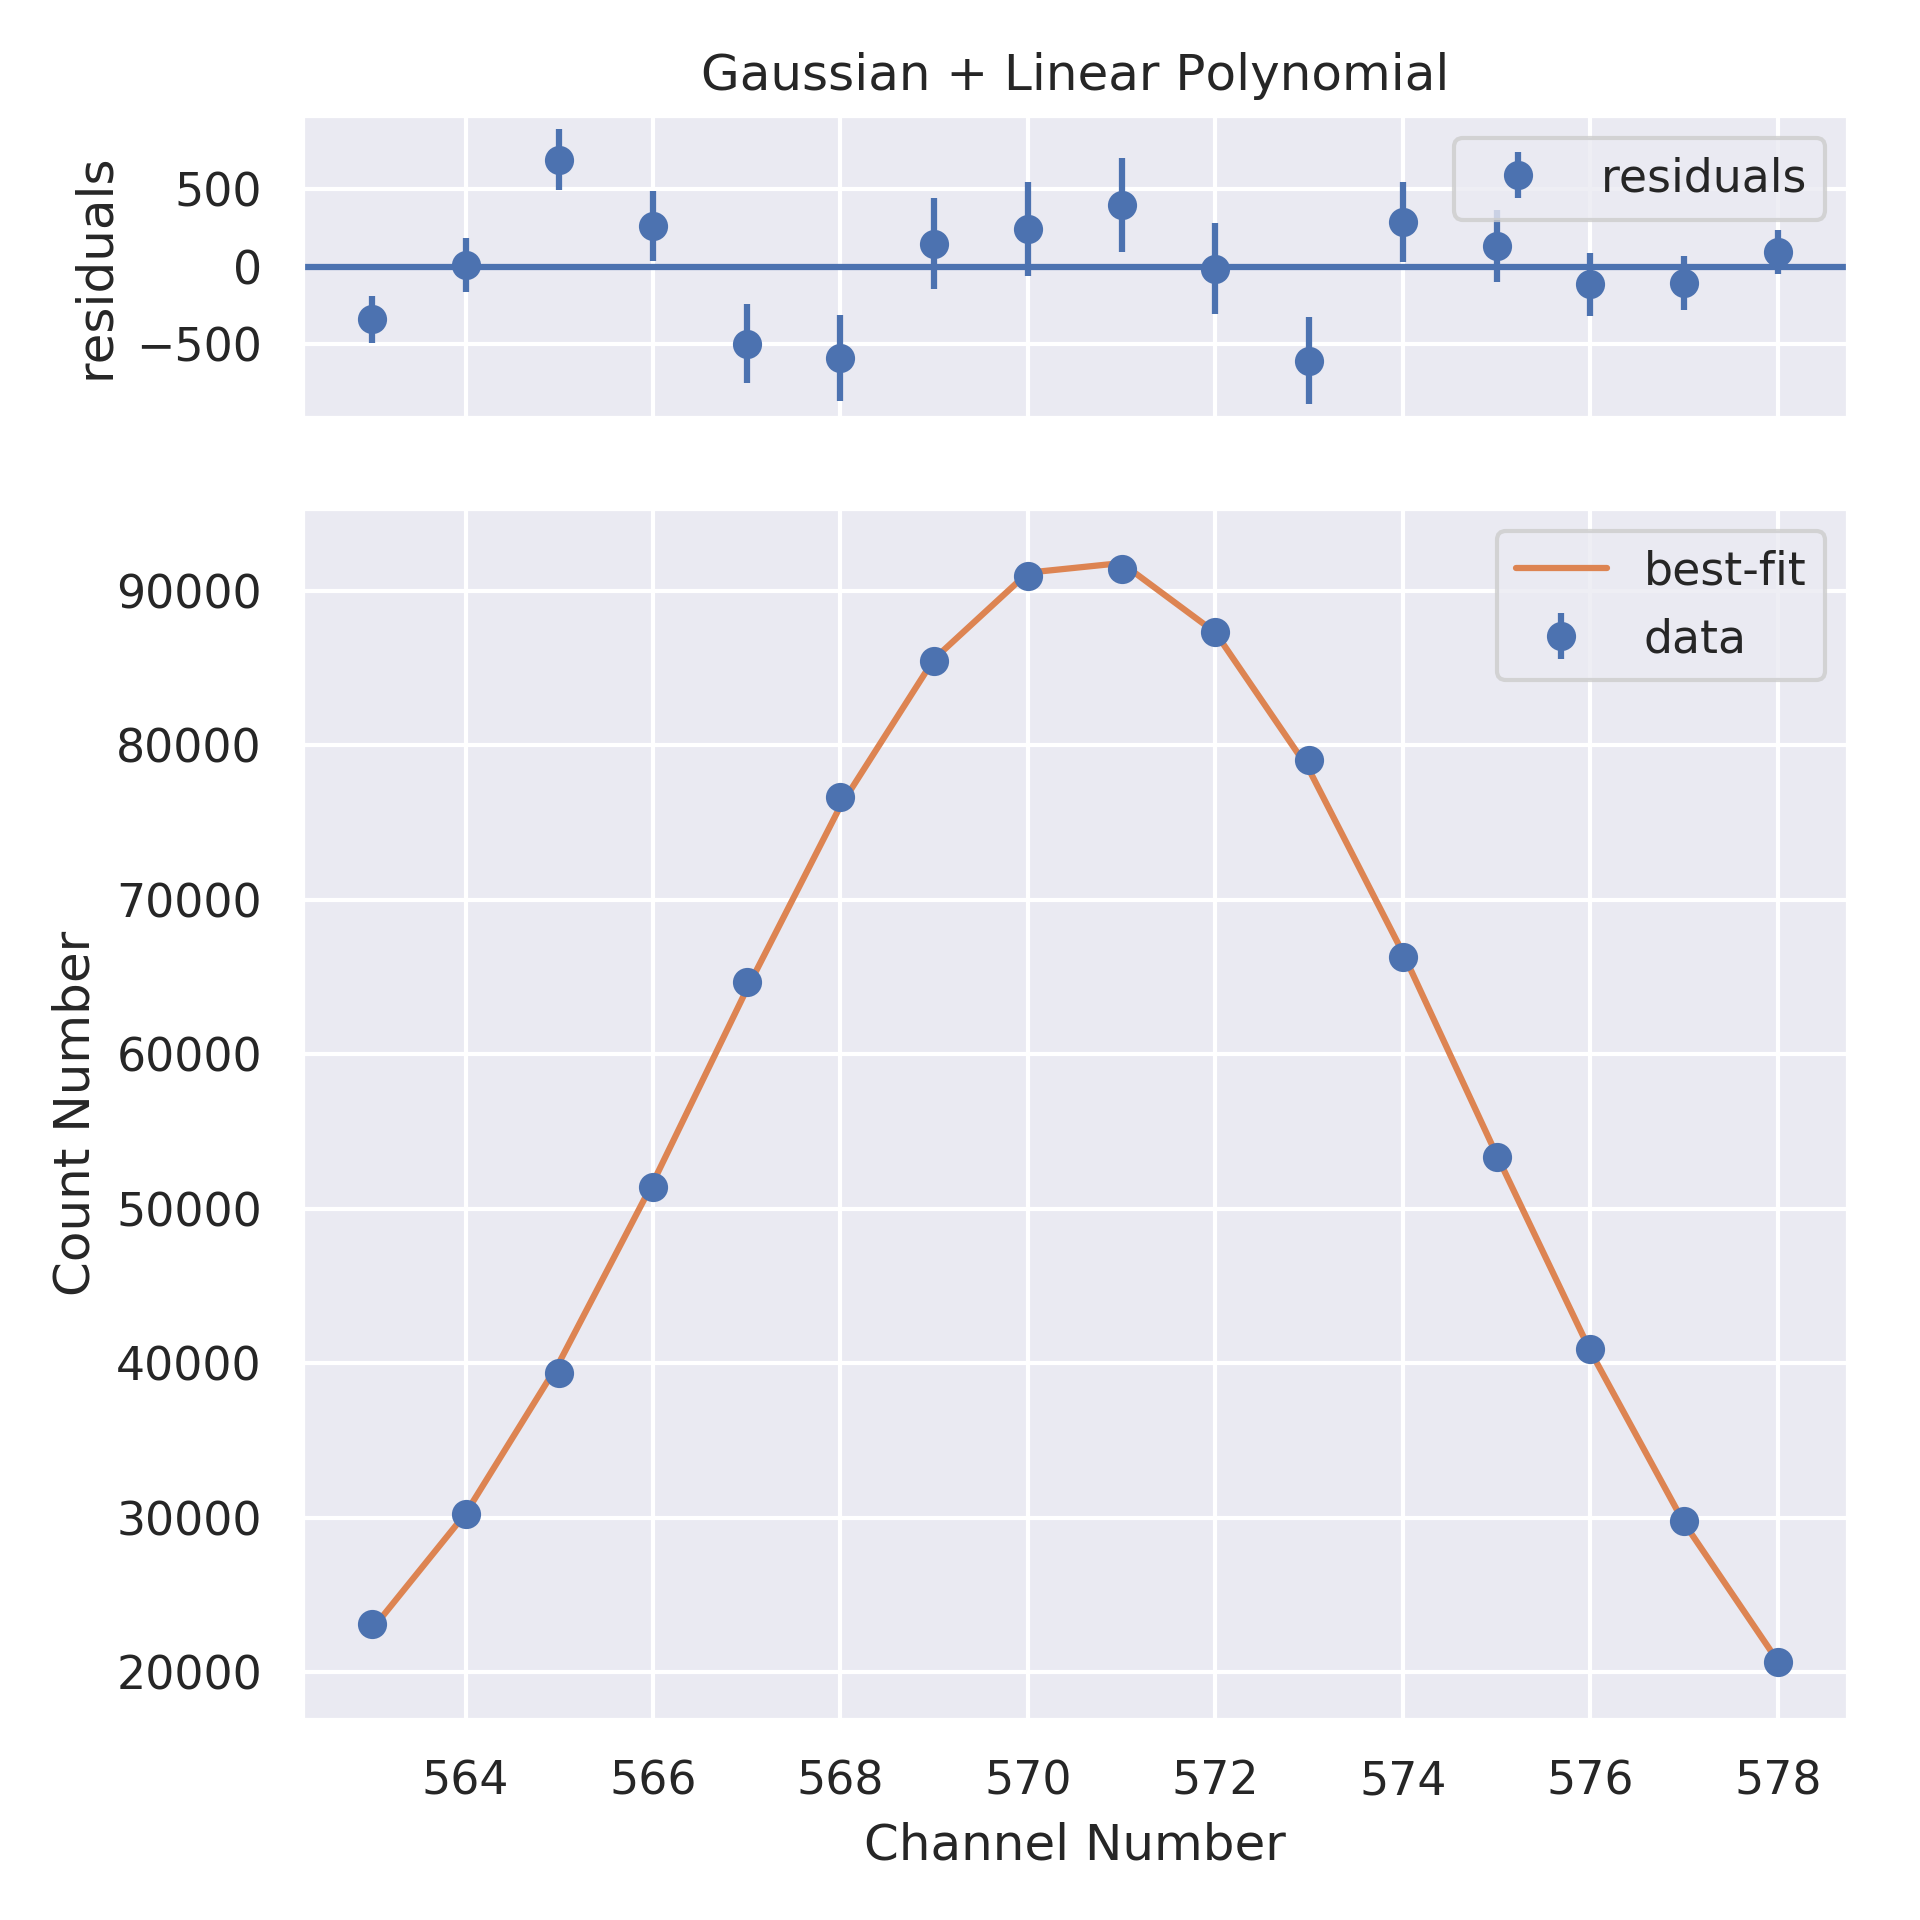
\includegraphics[width=\linewidth]{./Images/Barium133/Linear/Linear_1_Zoom.png}
    \caption{Zoomed in peak with fit}
    %\label{fig:sub2}
  \end{subfigure}
  \caption{Fit of full \& zoomed in peak of \element{Ba}{133} 81 keV peak}
  %\label{fig:test}
\end{figure}
\begin{figure}[H]
  \centering
  \begin{subfigure}{.5\linewidth}
    \centering
    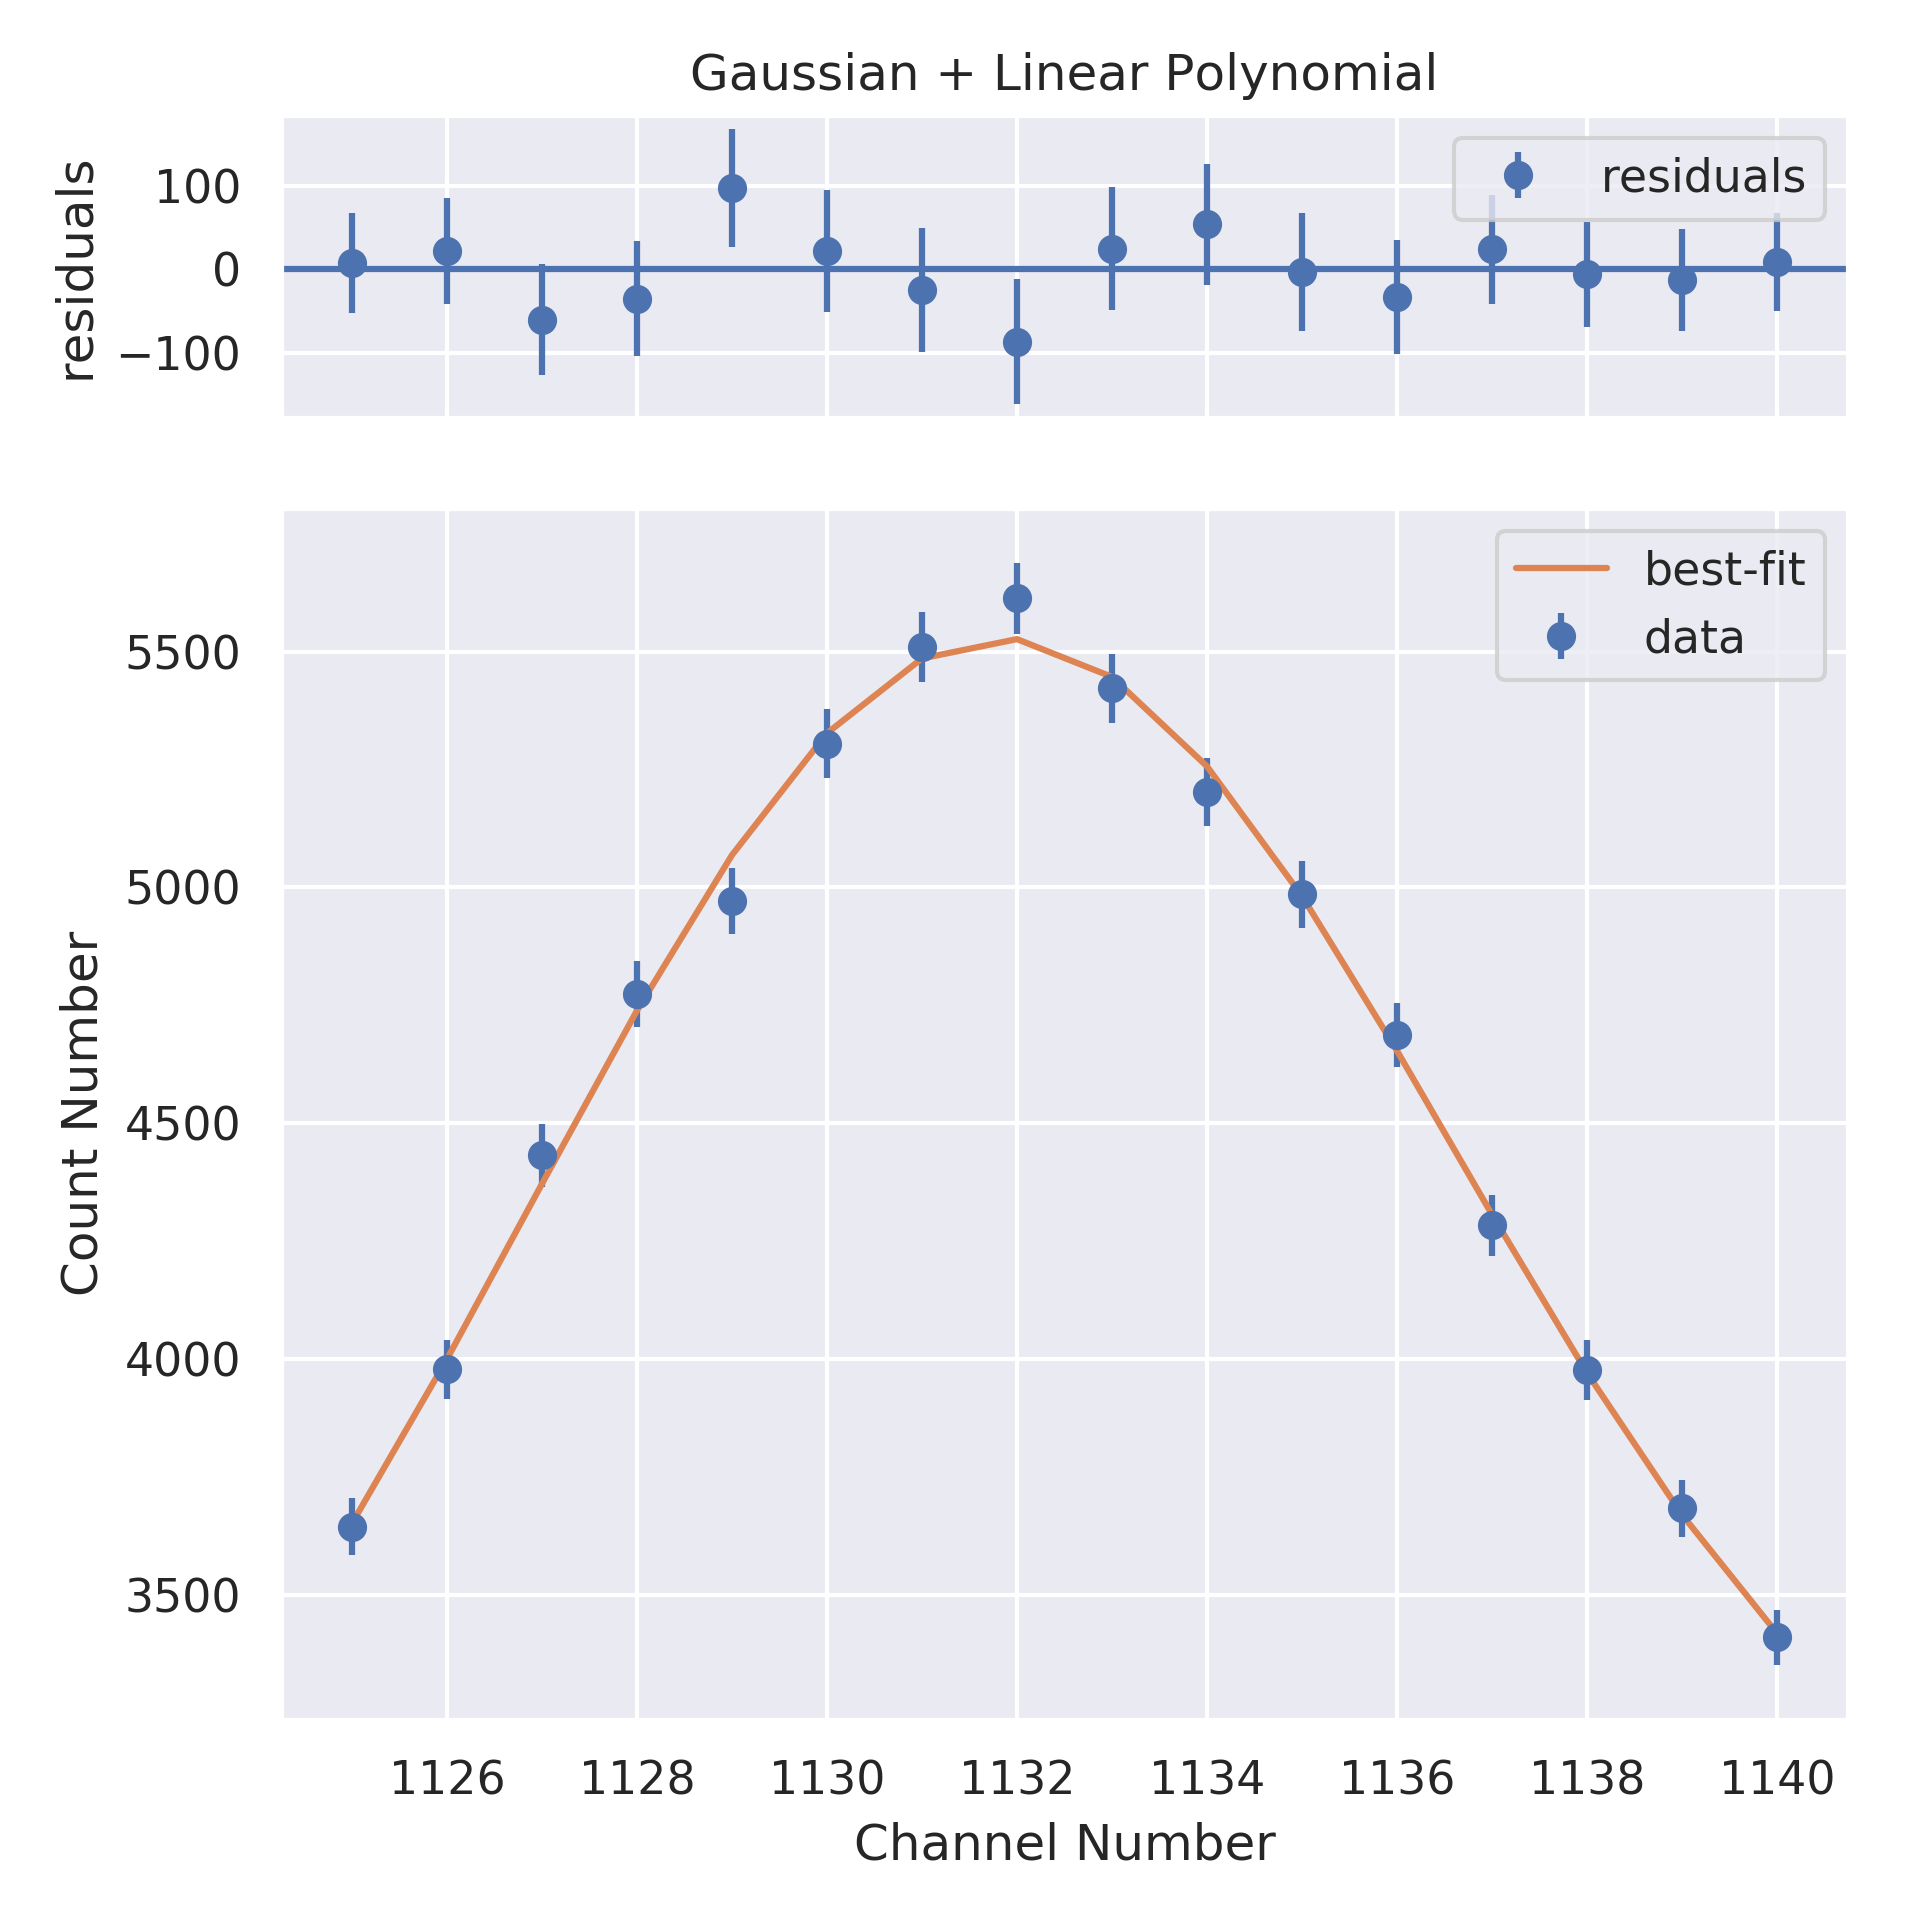
\includegraphics[width=\linewidth]{./Images/Barium133/Linear/Linear_2_Full.png}
    \caption{Full peak with fit}
    %\label{fig:sub1}
  \end{subfigure}%
  \begin{subfigure}{.5\linewidth}
    \centering
    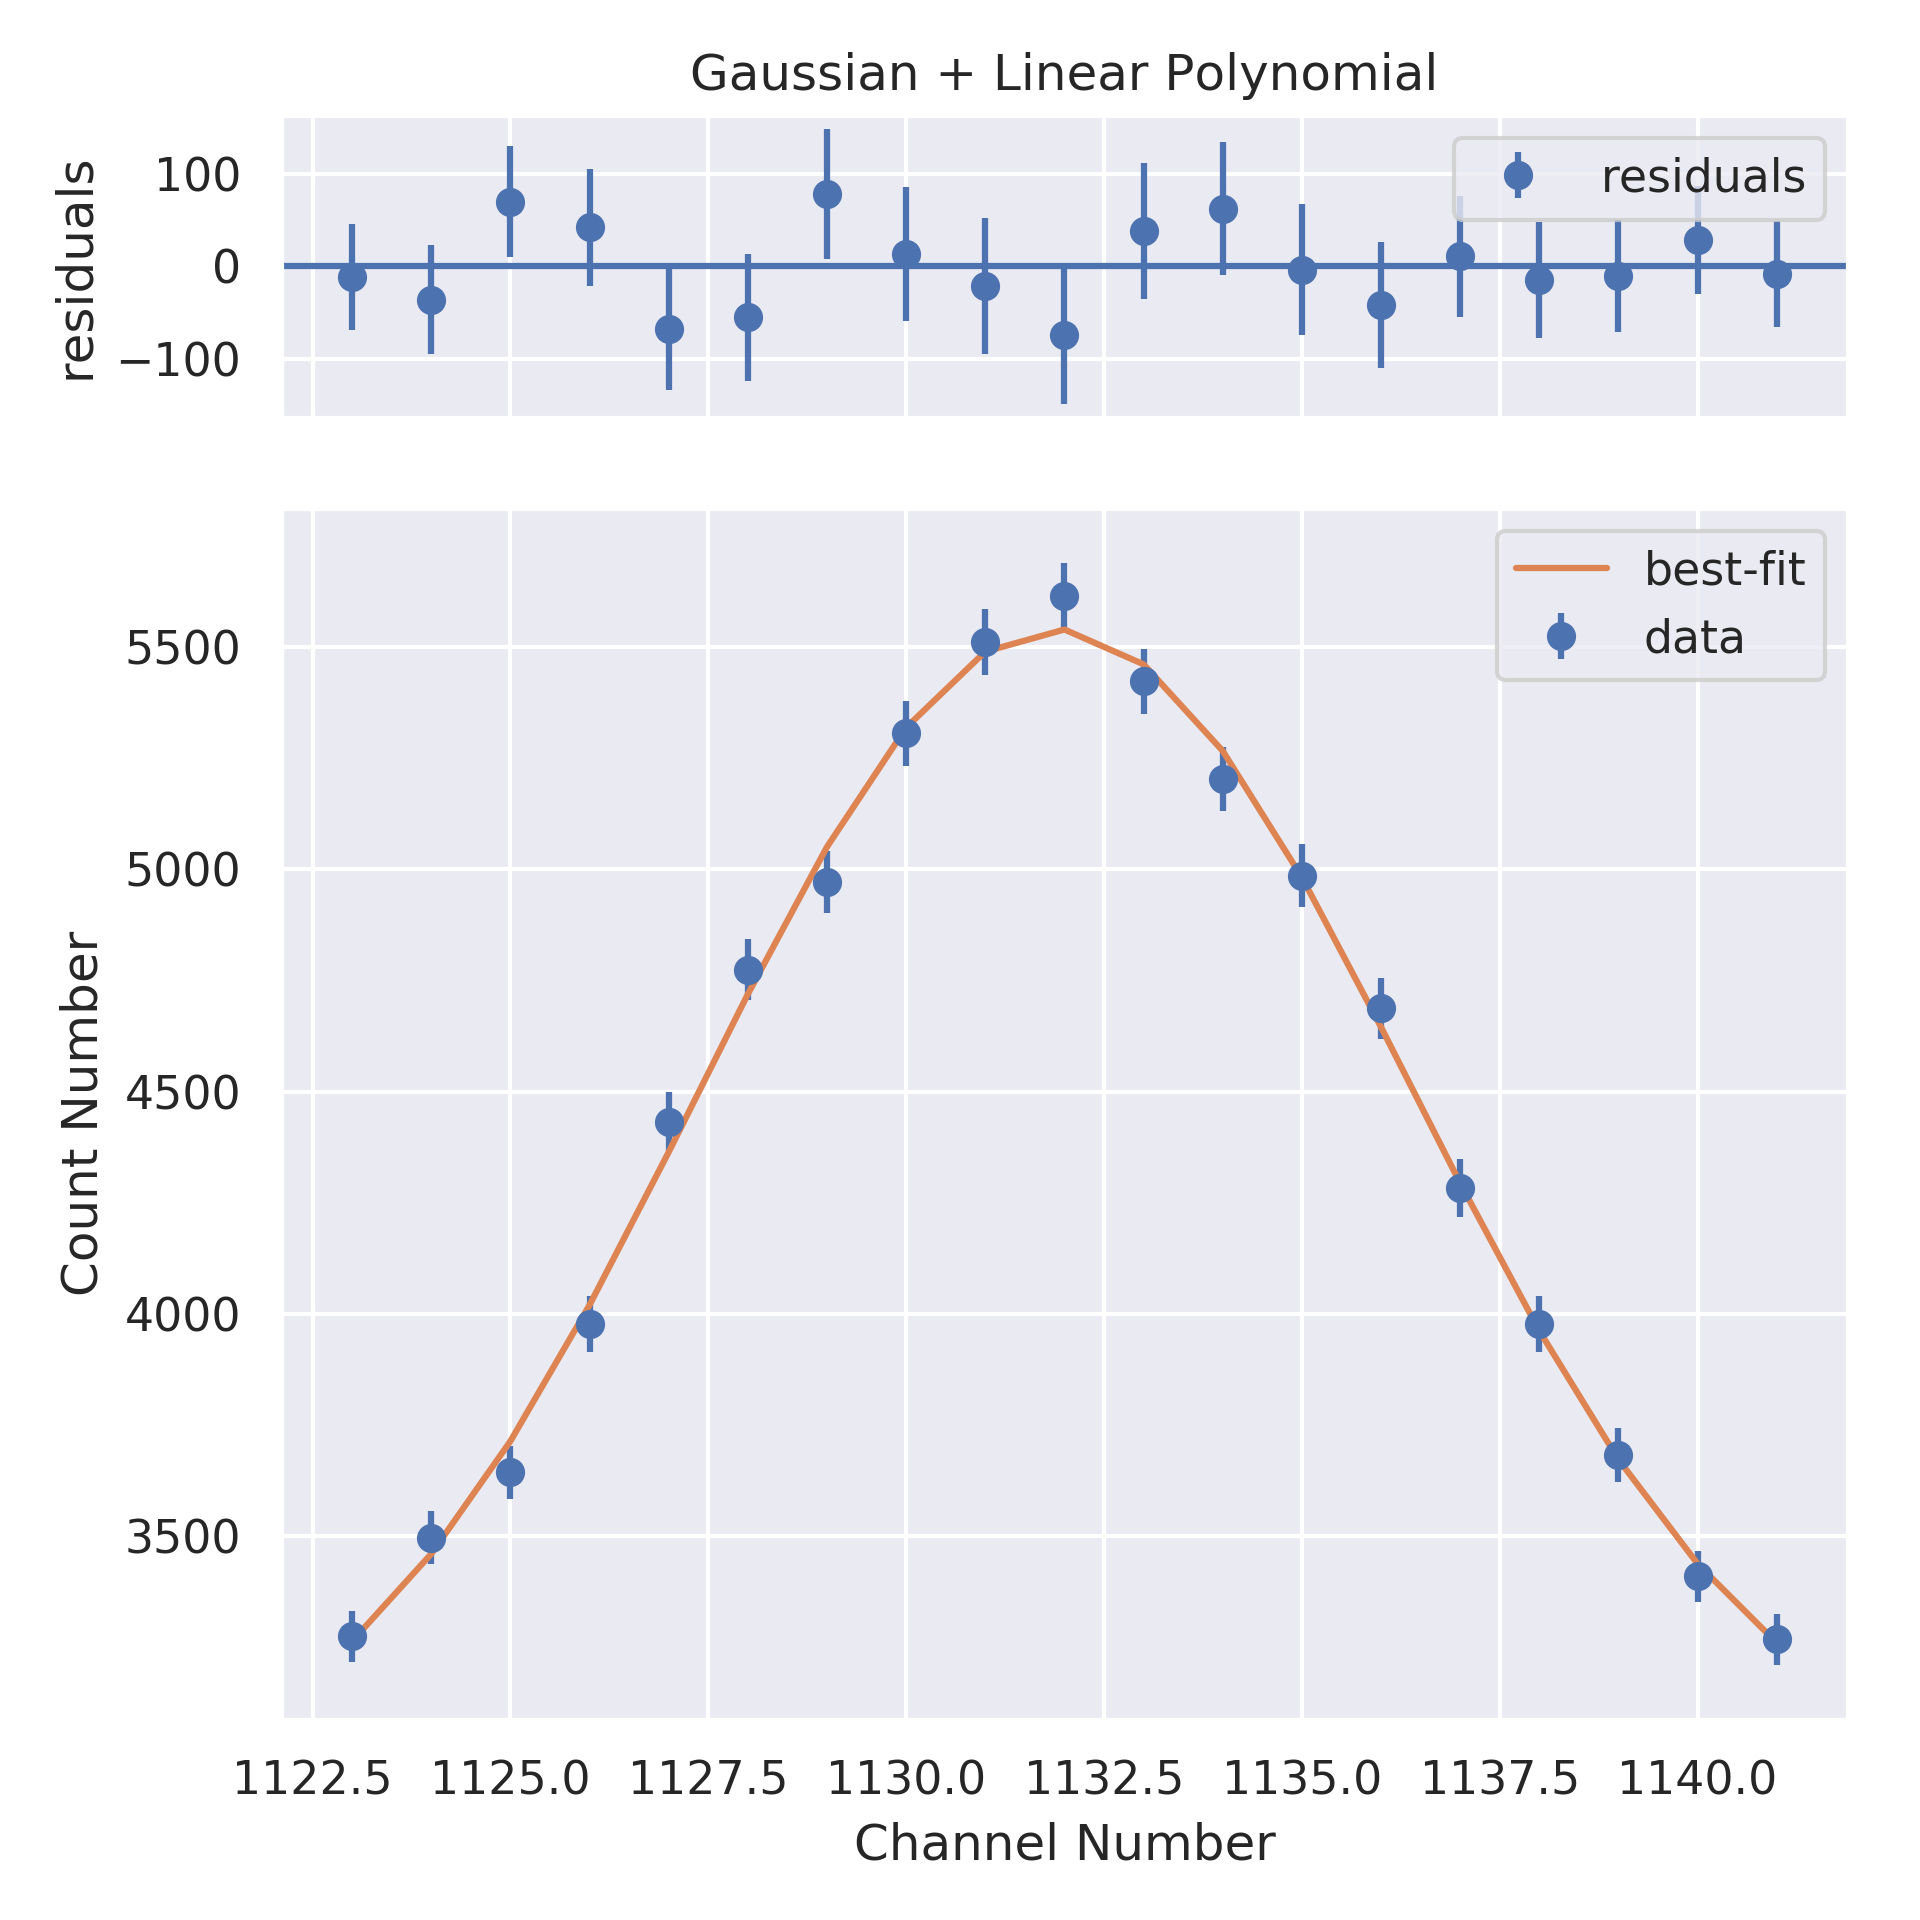
\includegraphics[width=\linewidth]{./Images/Barium133/Linear/Linear_2_Zoom.png}
    \caption{Zoomed in peak with fit}
    %\label{fig:sub2}
  \end{subfigure}
  \caption{Fit of full \& zoomed in peak of \element{Ba}{133} 161 keV peak}
  %\label{fig:test}
\end{figure}
\begin{figure}[H]
  \centering
  \begin{subfigure}{.5\linewidth}
    \centering
    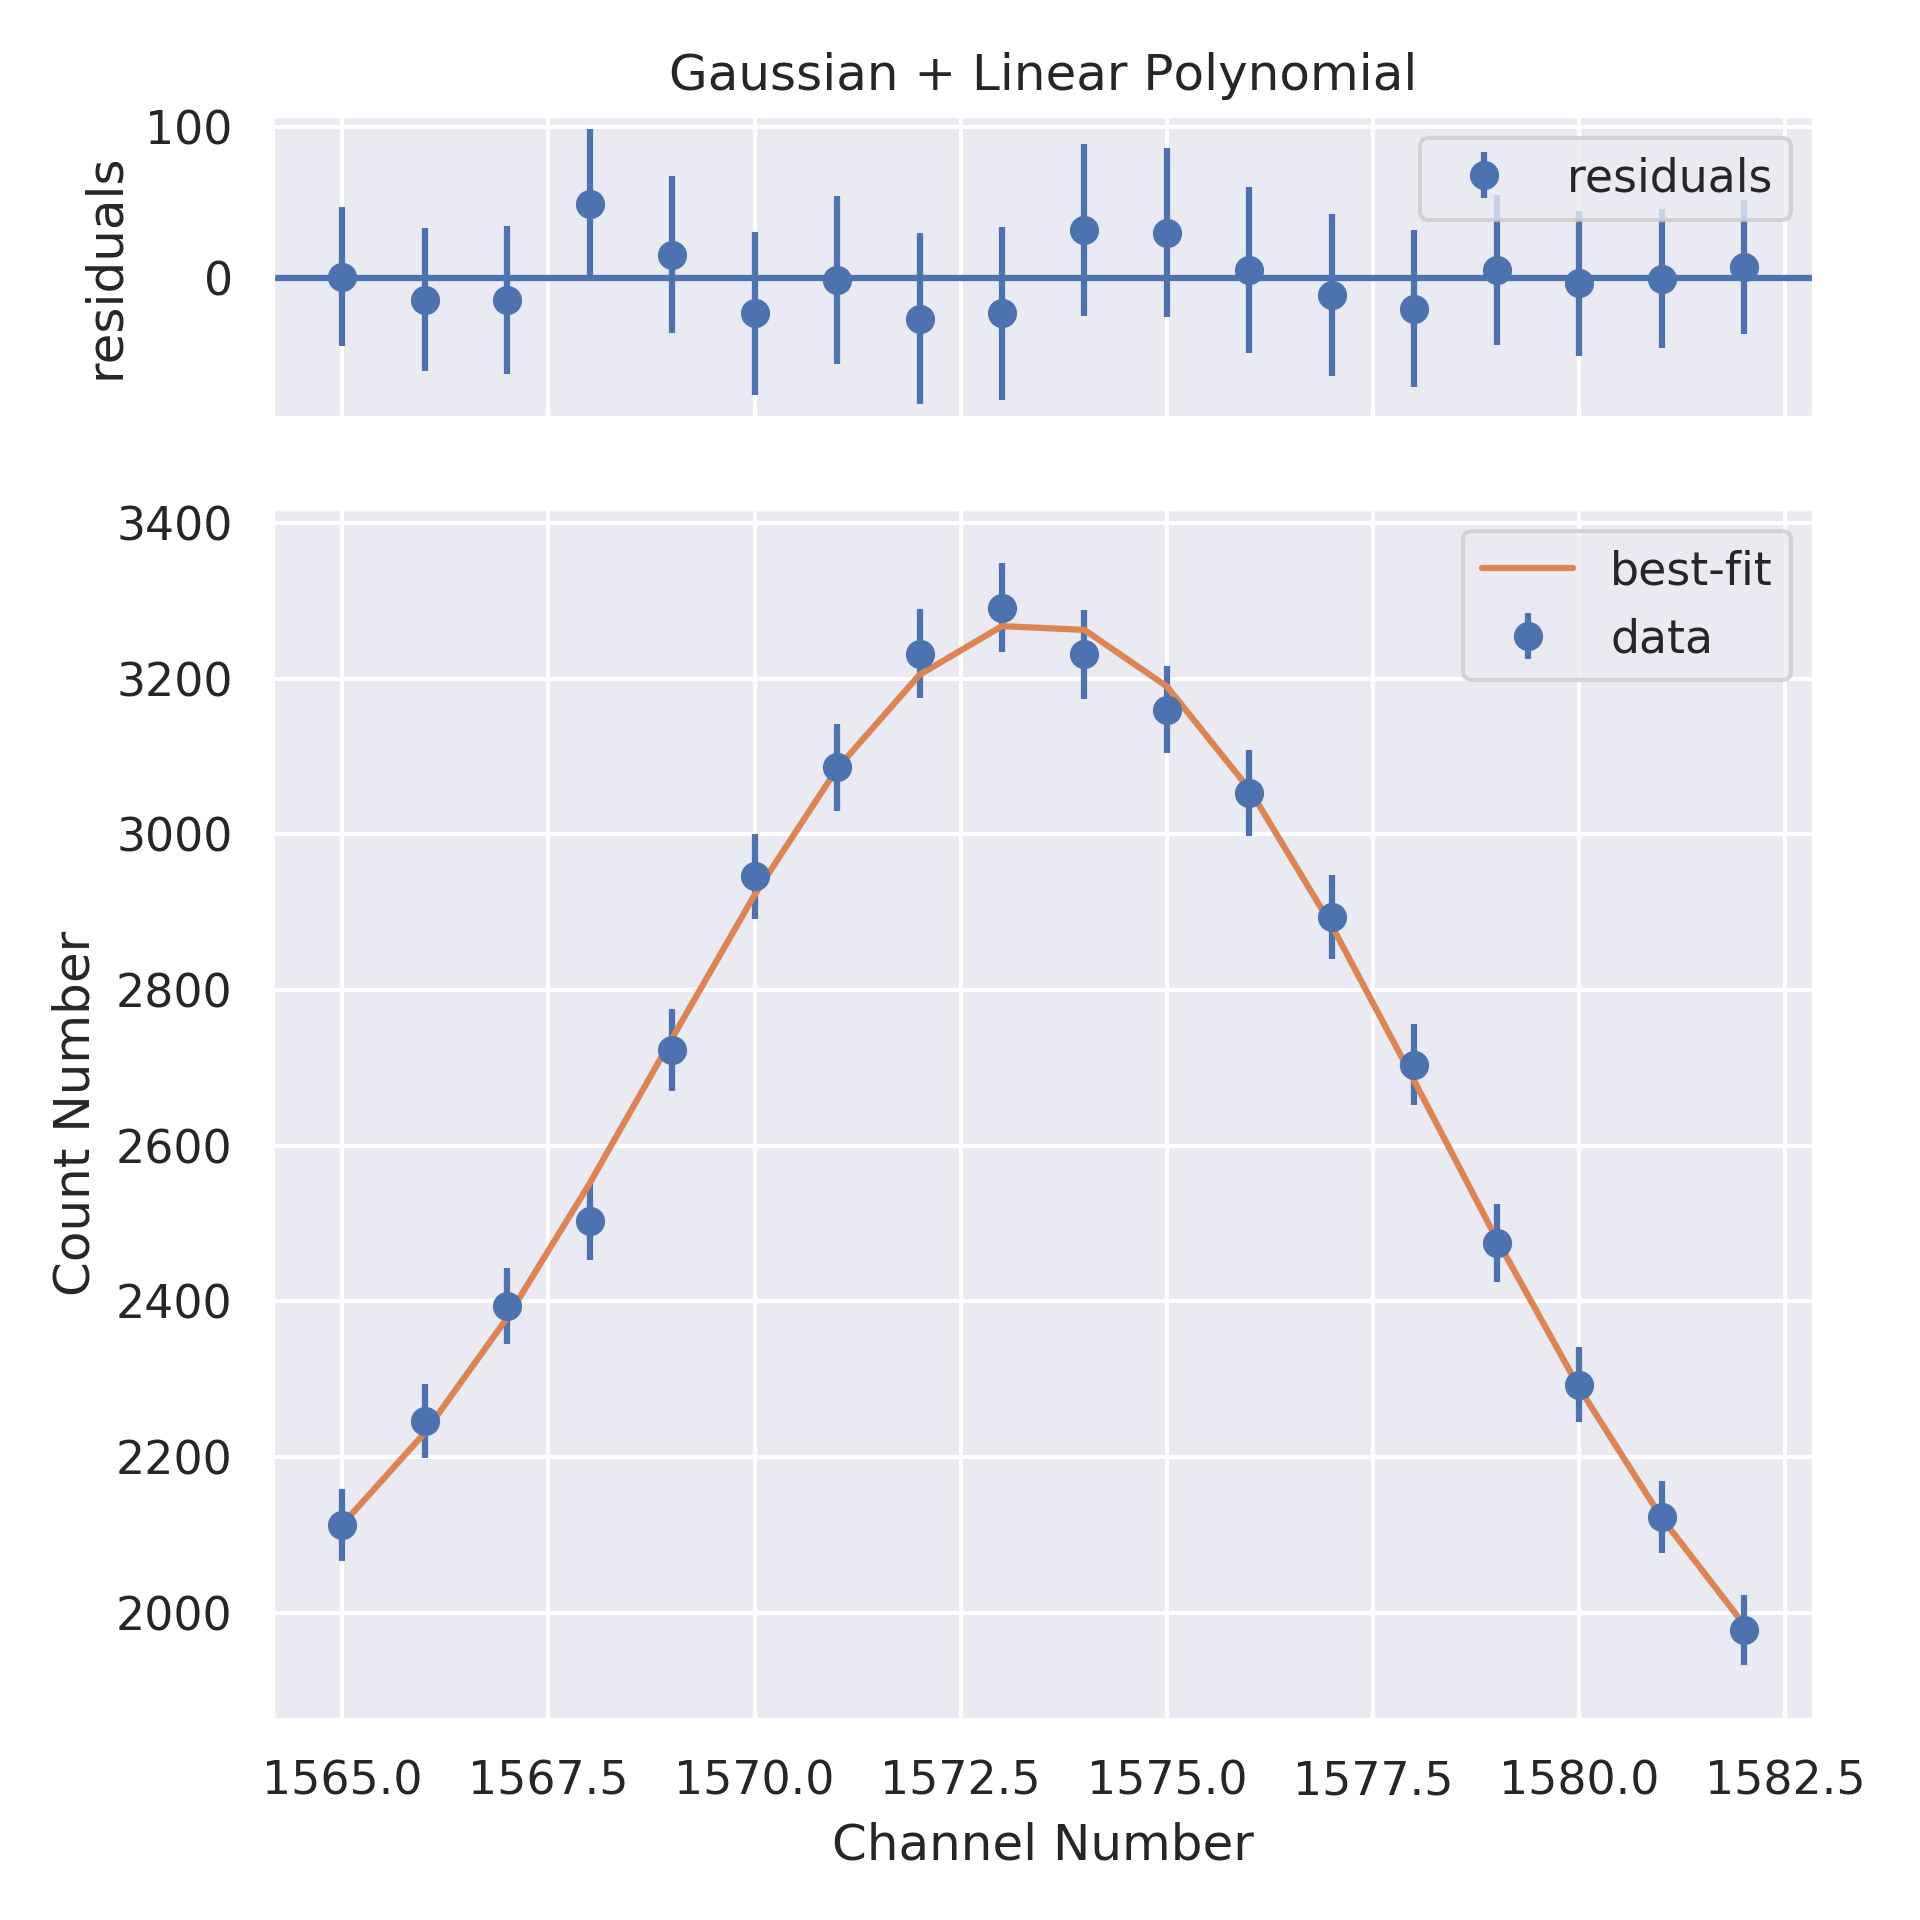
\includegraphics[width=\linewidth]{./Images/Barium133/Linear/Linear_3_Full.png}
    \caption{Full peak with fit}
    %\label{fig:sub1}
  \end{subfigure}%
  \begin{subfigure}{.5\linewidth}
    \centering
    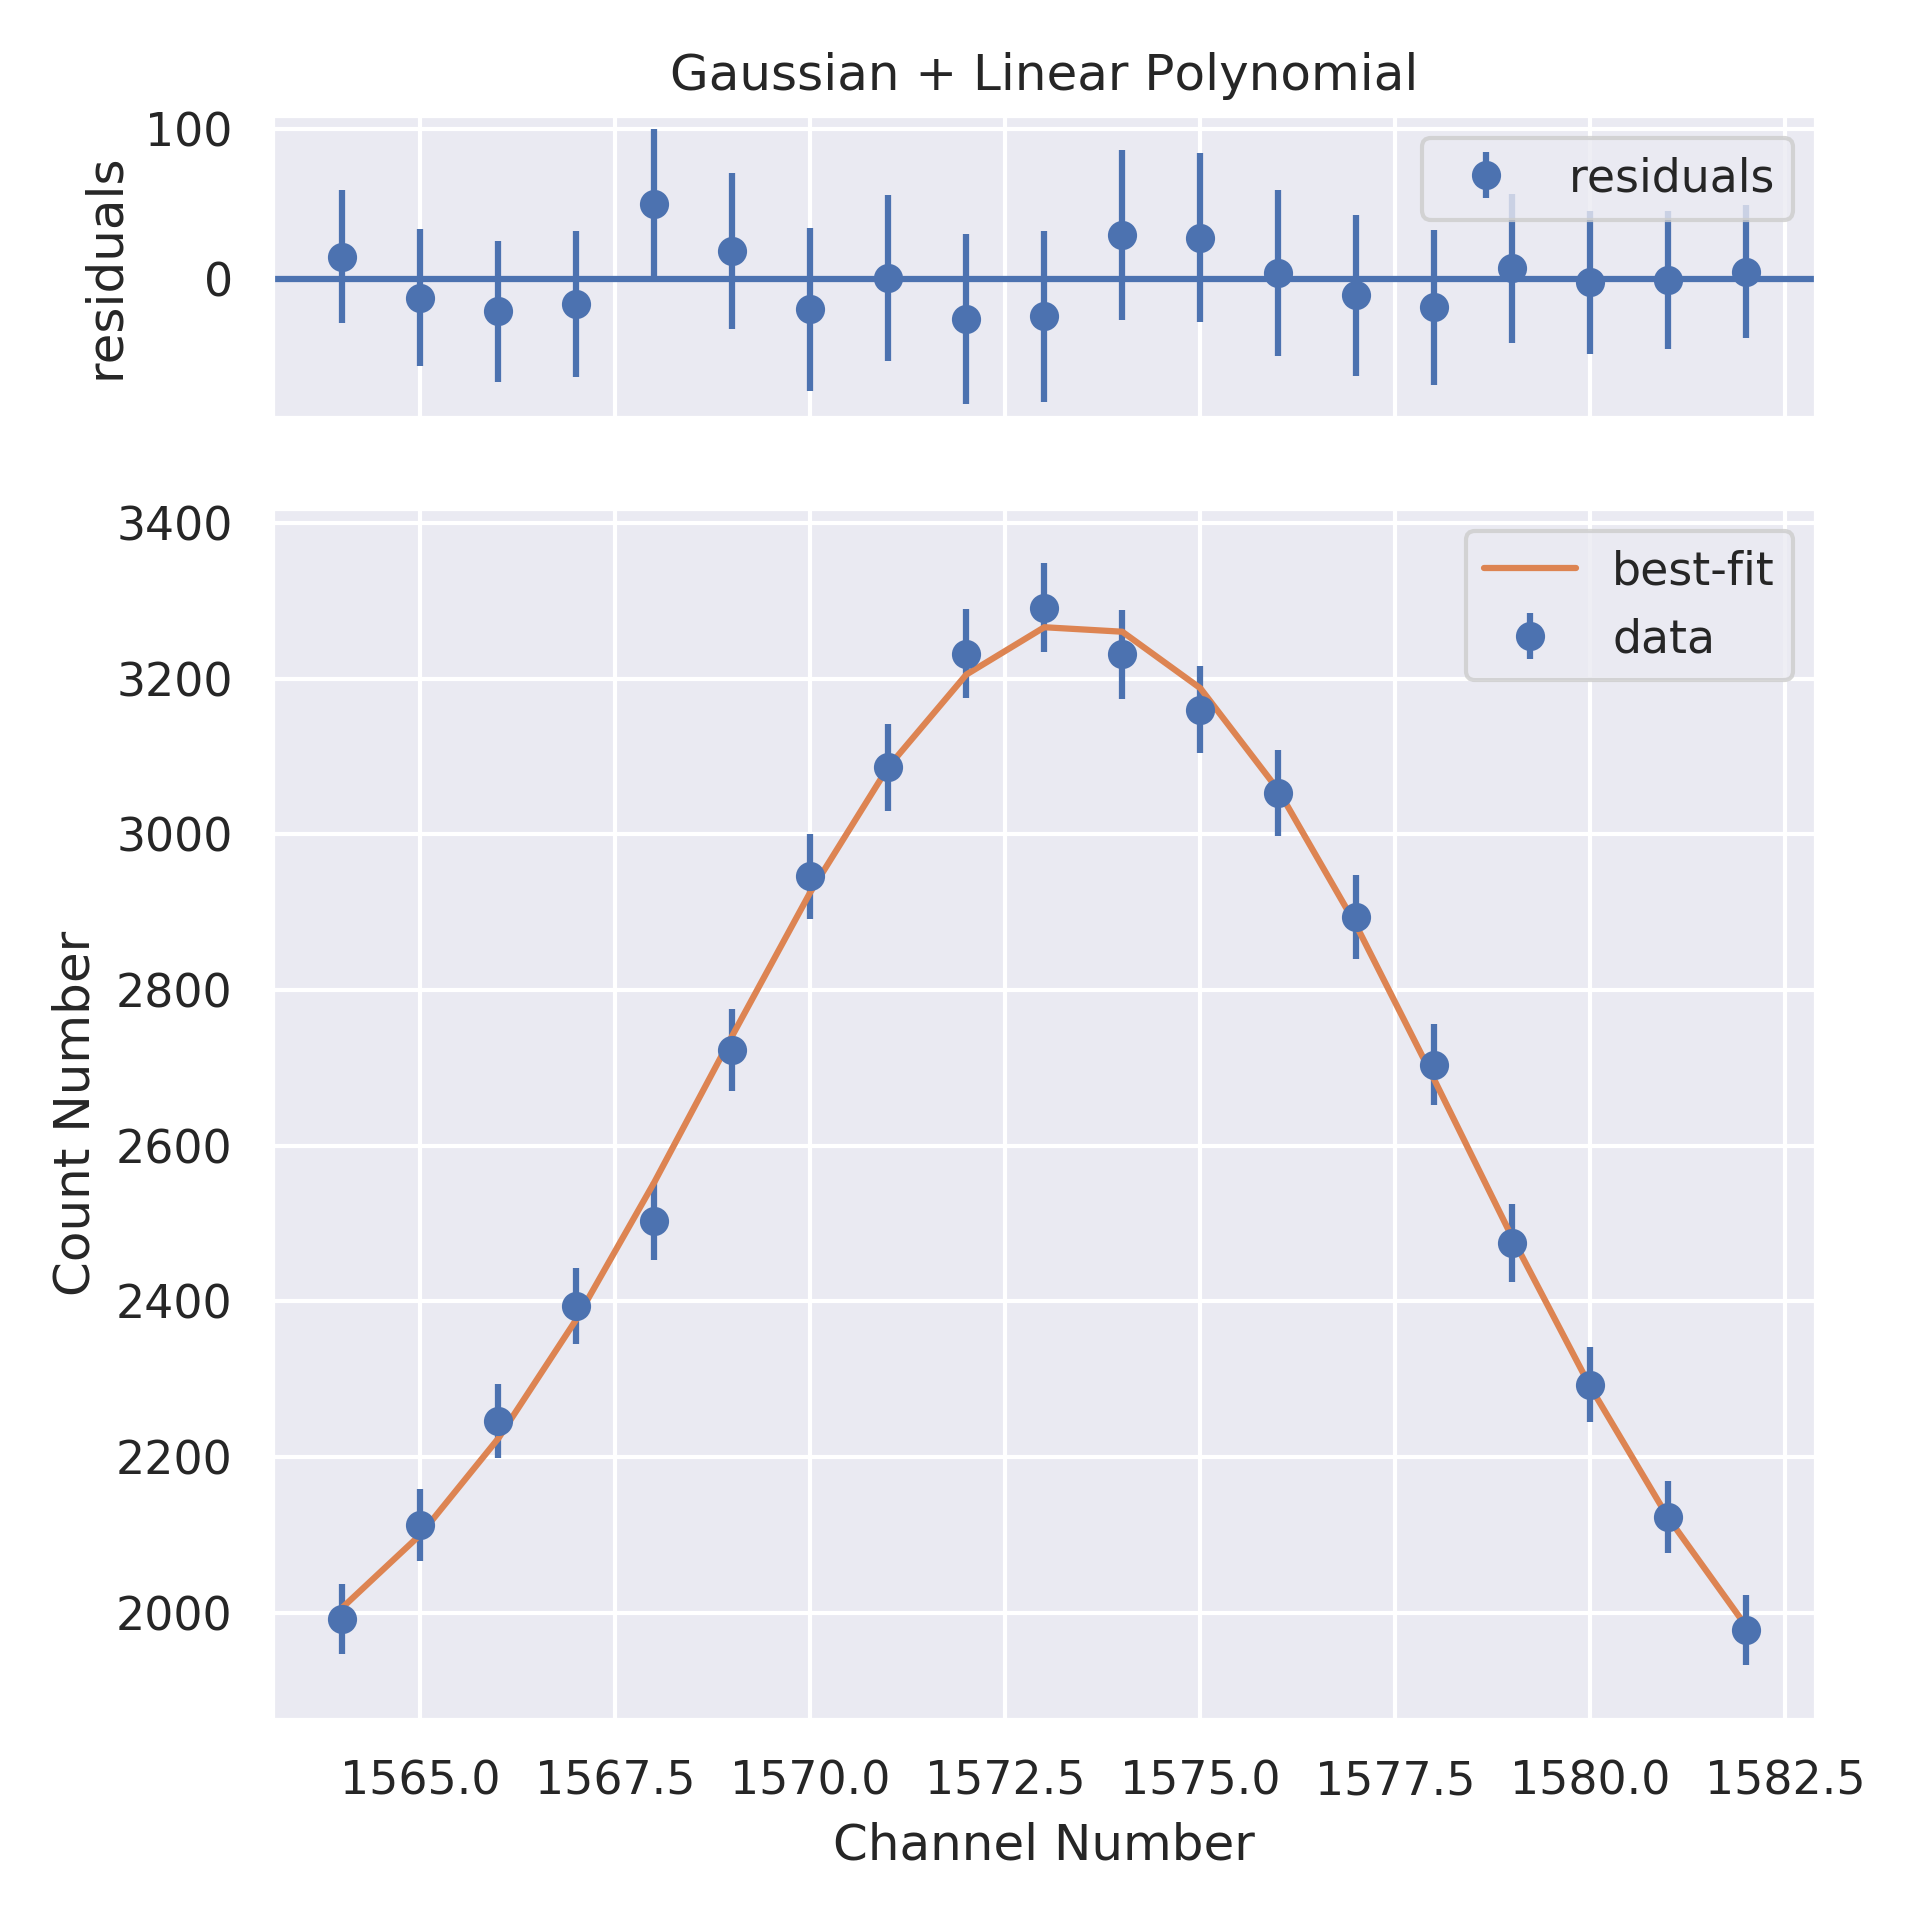
\includegraphics[width=\linewidth]{./Images/Barium133/Linear/Linear_3_Zoom.png}
    \caption{Zoomed in peak with fit}
    %\label{fig:sub2}
  \end{subfigure}
  \caption{Fit of full \& zoomed in peak of \element{Ba}{133} 223 keV peak}
  %\label{fig:test}
\end{figure}
\begin{figure}[H]
  \centering
  \begin{subfigure}{.5\linewidth}
    \centering
    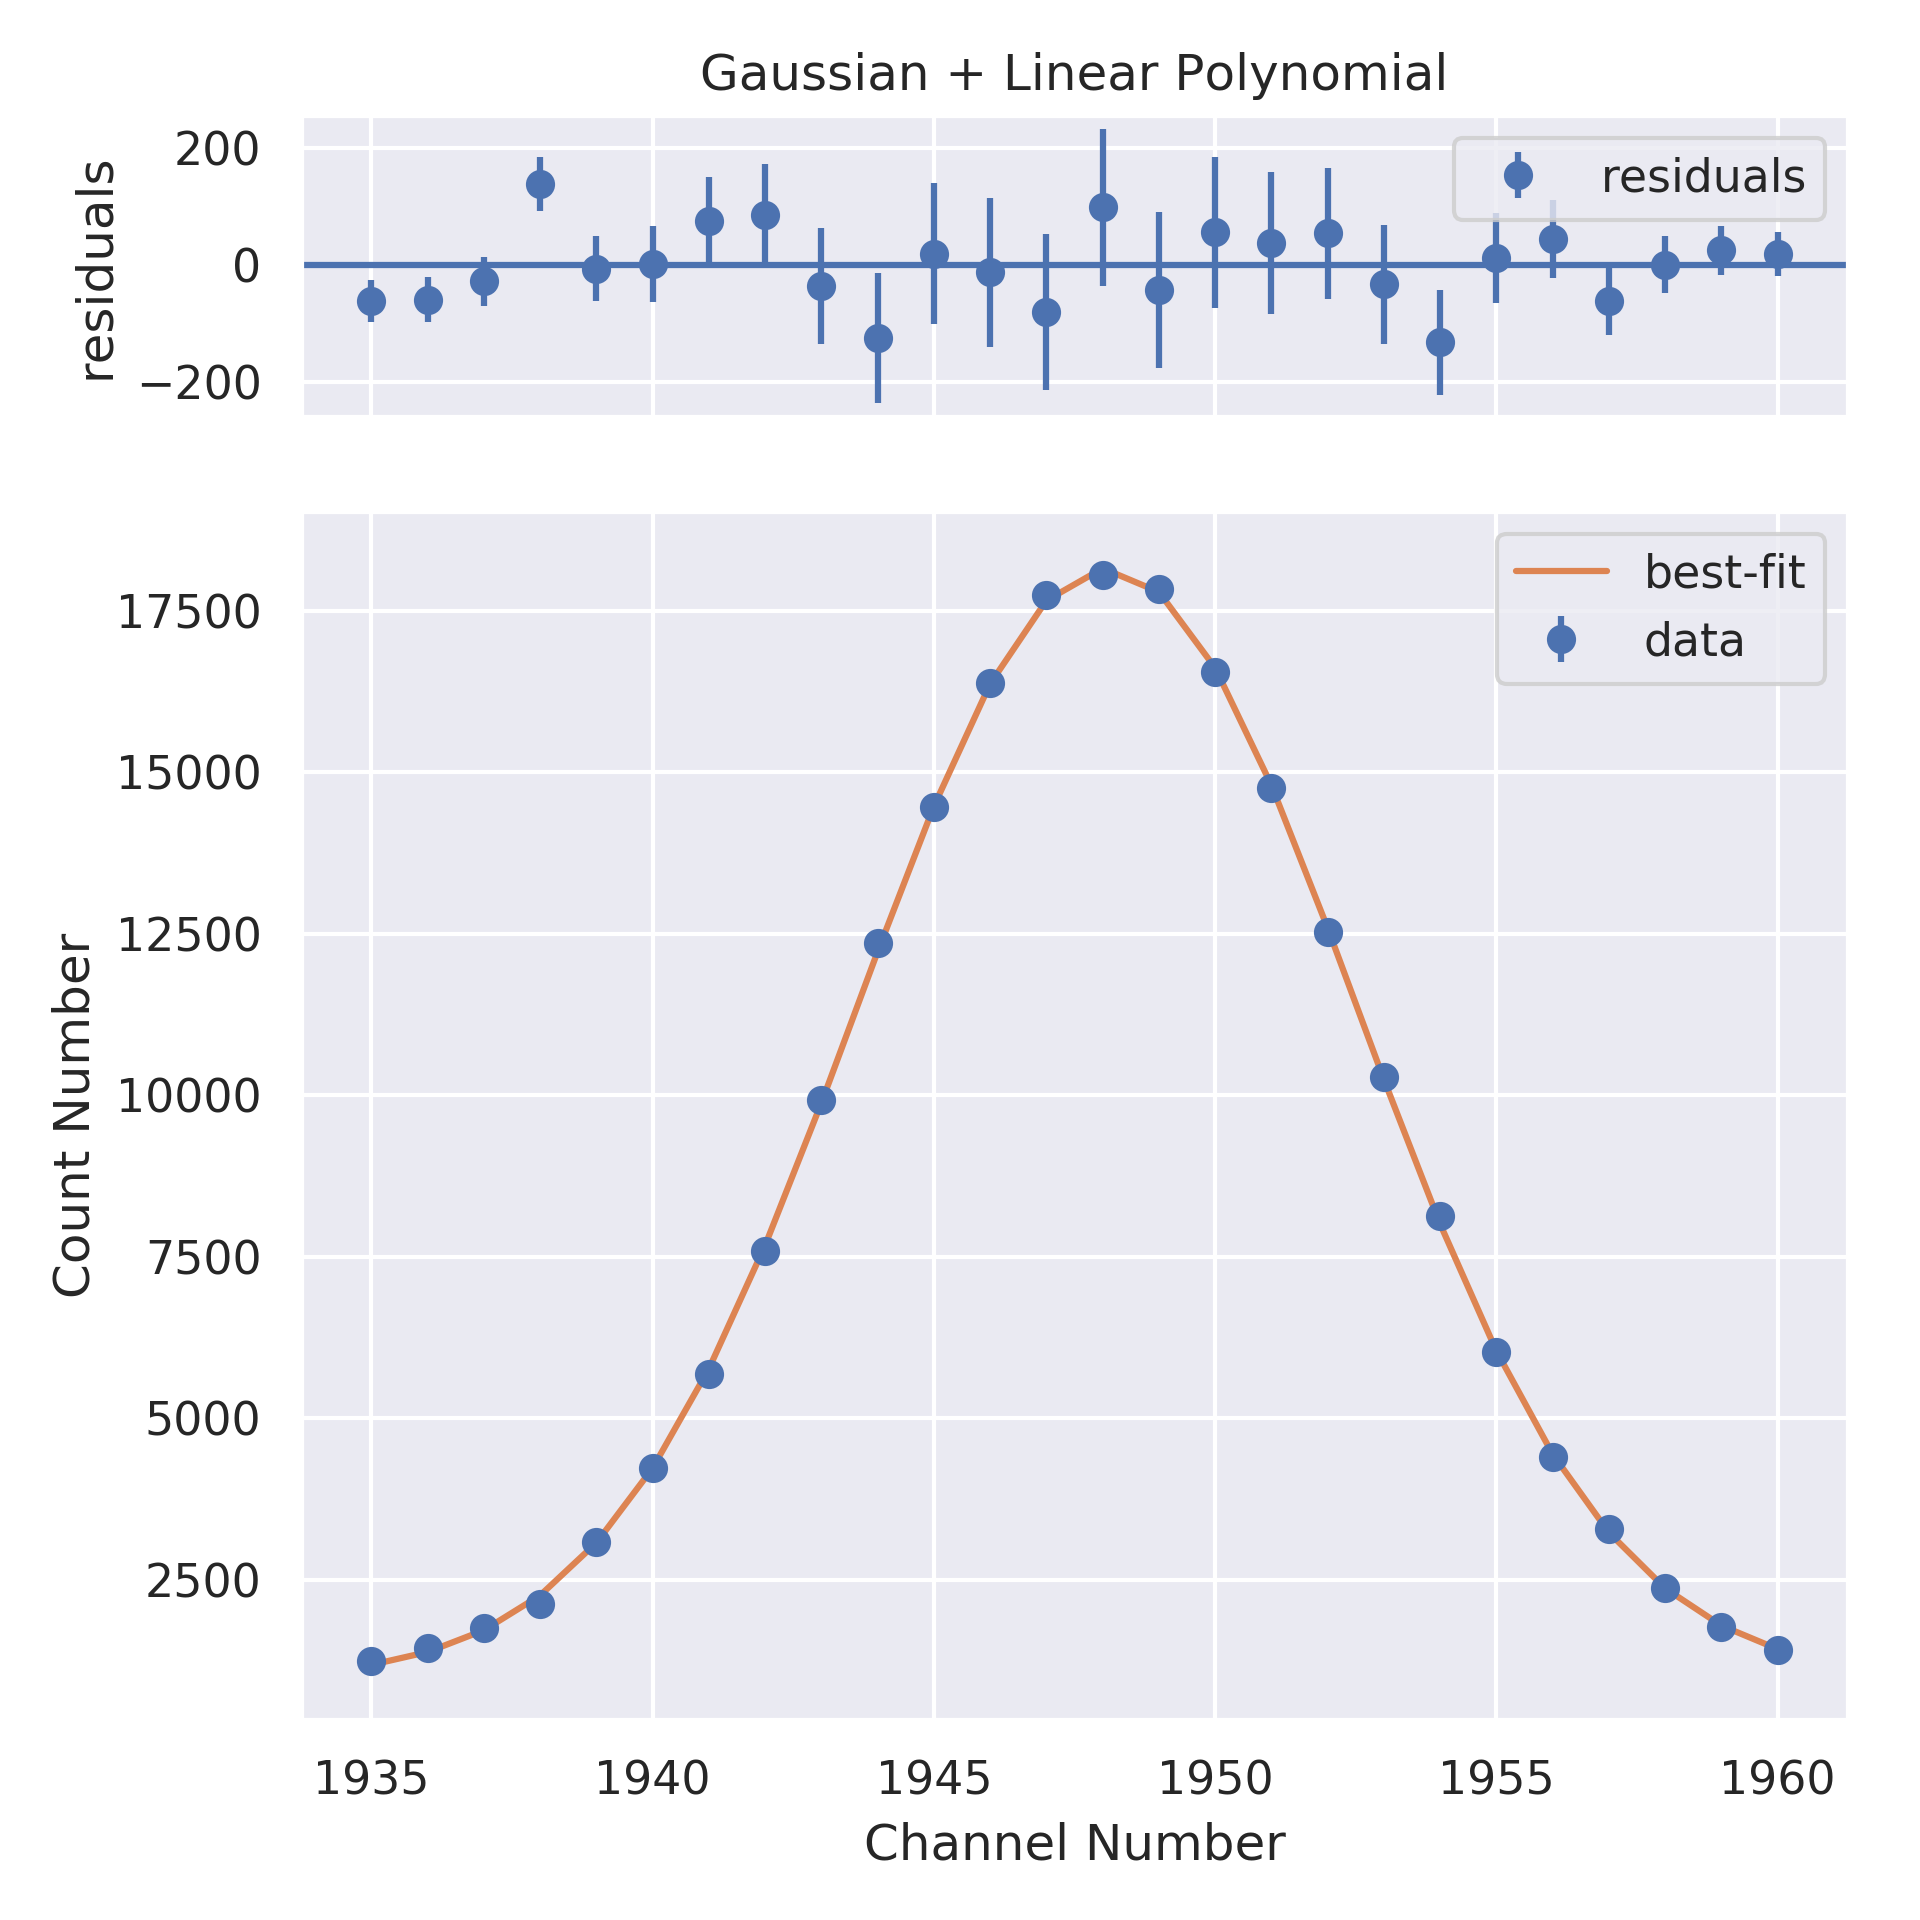
\includegraphics[width=\linewidth]{./Images/Barium133/Linear/Linear_4_Full.png}
    \caption{Full peak with fit}
    %\label{fig:sub1}
  \end{subfigure}%
  \begin{subfigure}{.5\linewidth}
    \centering
    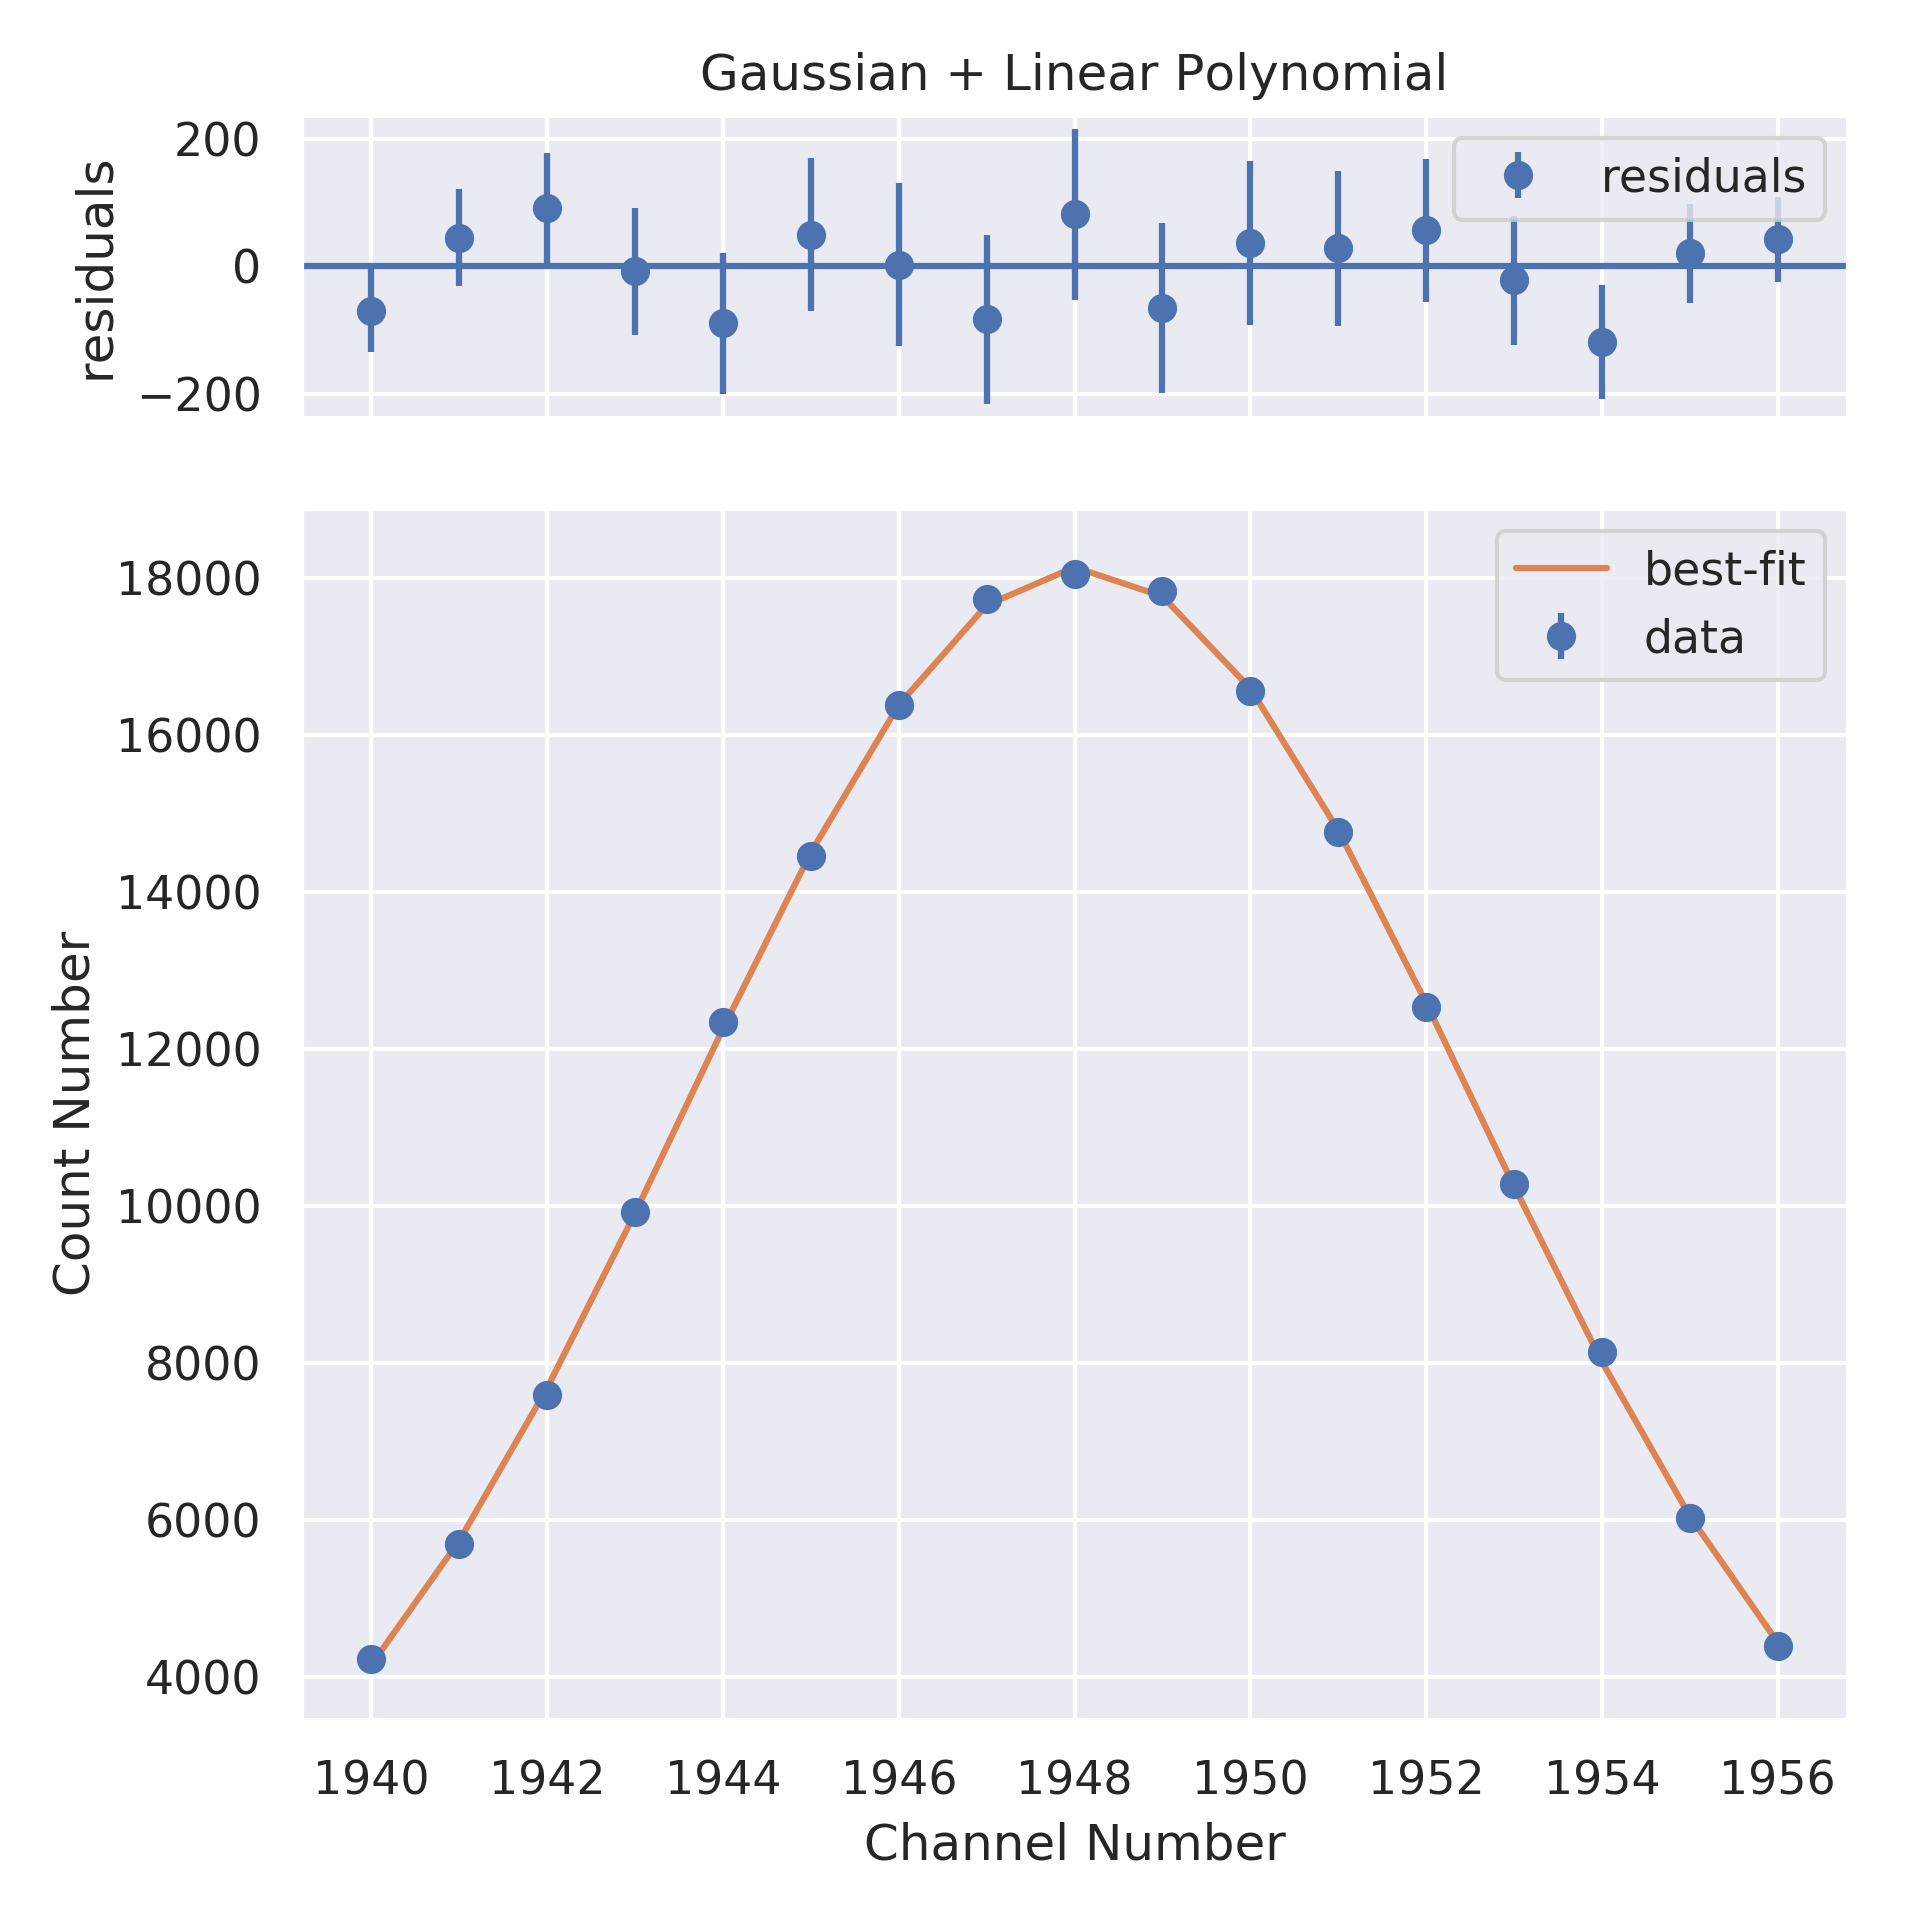
\includegraphics[width=\linewidth]{./Images/Barium133/Linear/Linear_4_Zoom.png}
    \caption{Zoomed in peak with fit}
    %\label{fig:sub2}
  \end{subfigure}
  \caption{Fit of full \& zoomed in peak of \element{Ba}{133} 276 keV peak}
  %\label{fig:test}
\end{figure}
\begin{figure}[H]
  \centering
  \begin{subfigure}{.5\linewidth}
    \centering
    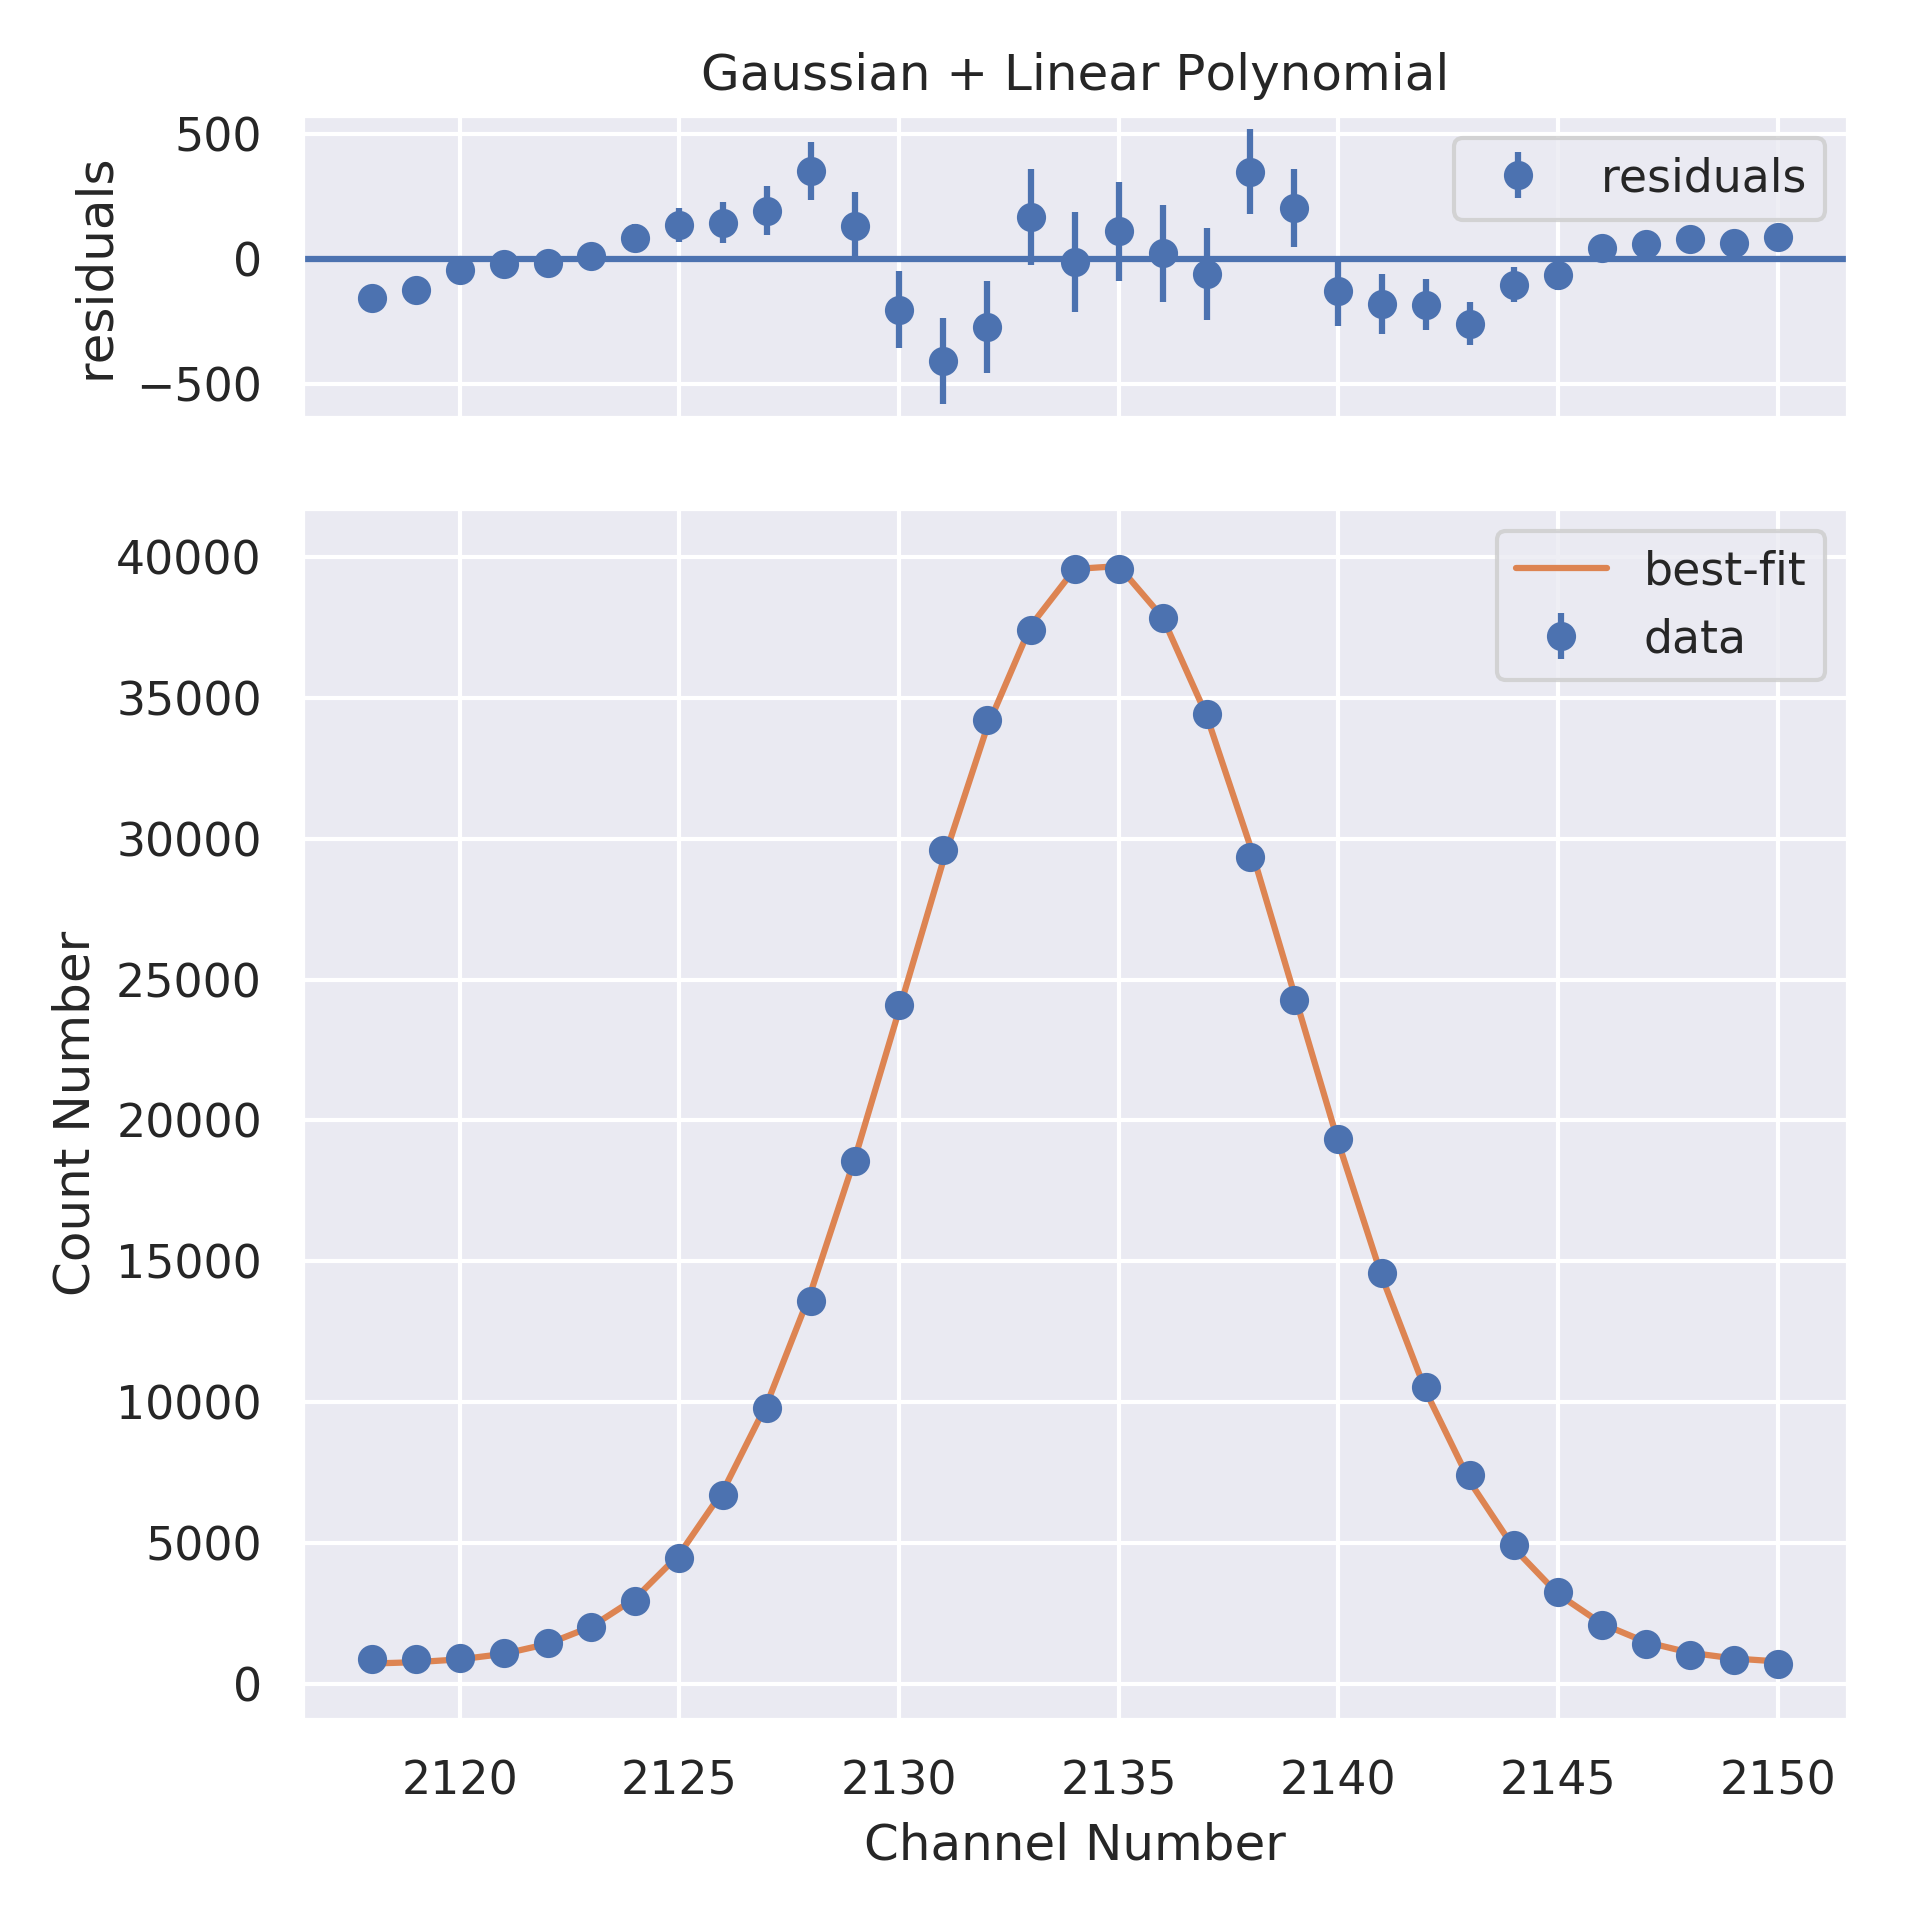
\includegraphics[width=\linewidth]{./Images/Barium133/Linear/Linear_5_Full.png}
    \caption{Full peak with fit}
    %\label{fig:sub1}
  \end{subfigure}%
  \begin{subfigure}{.5\linewidth}
    \centering
    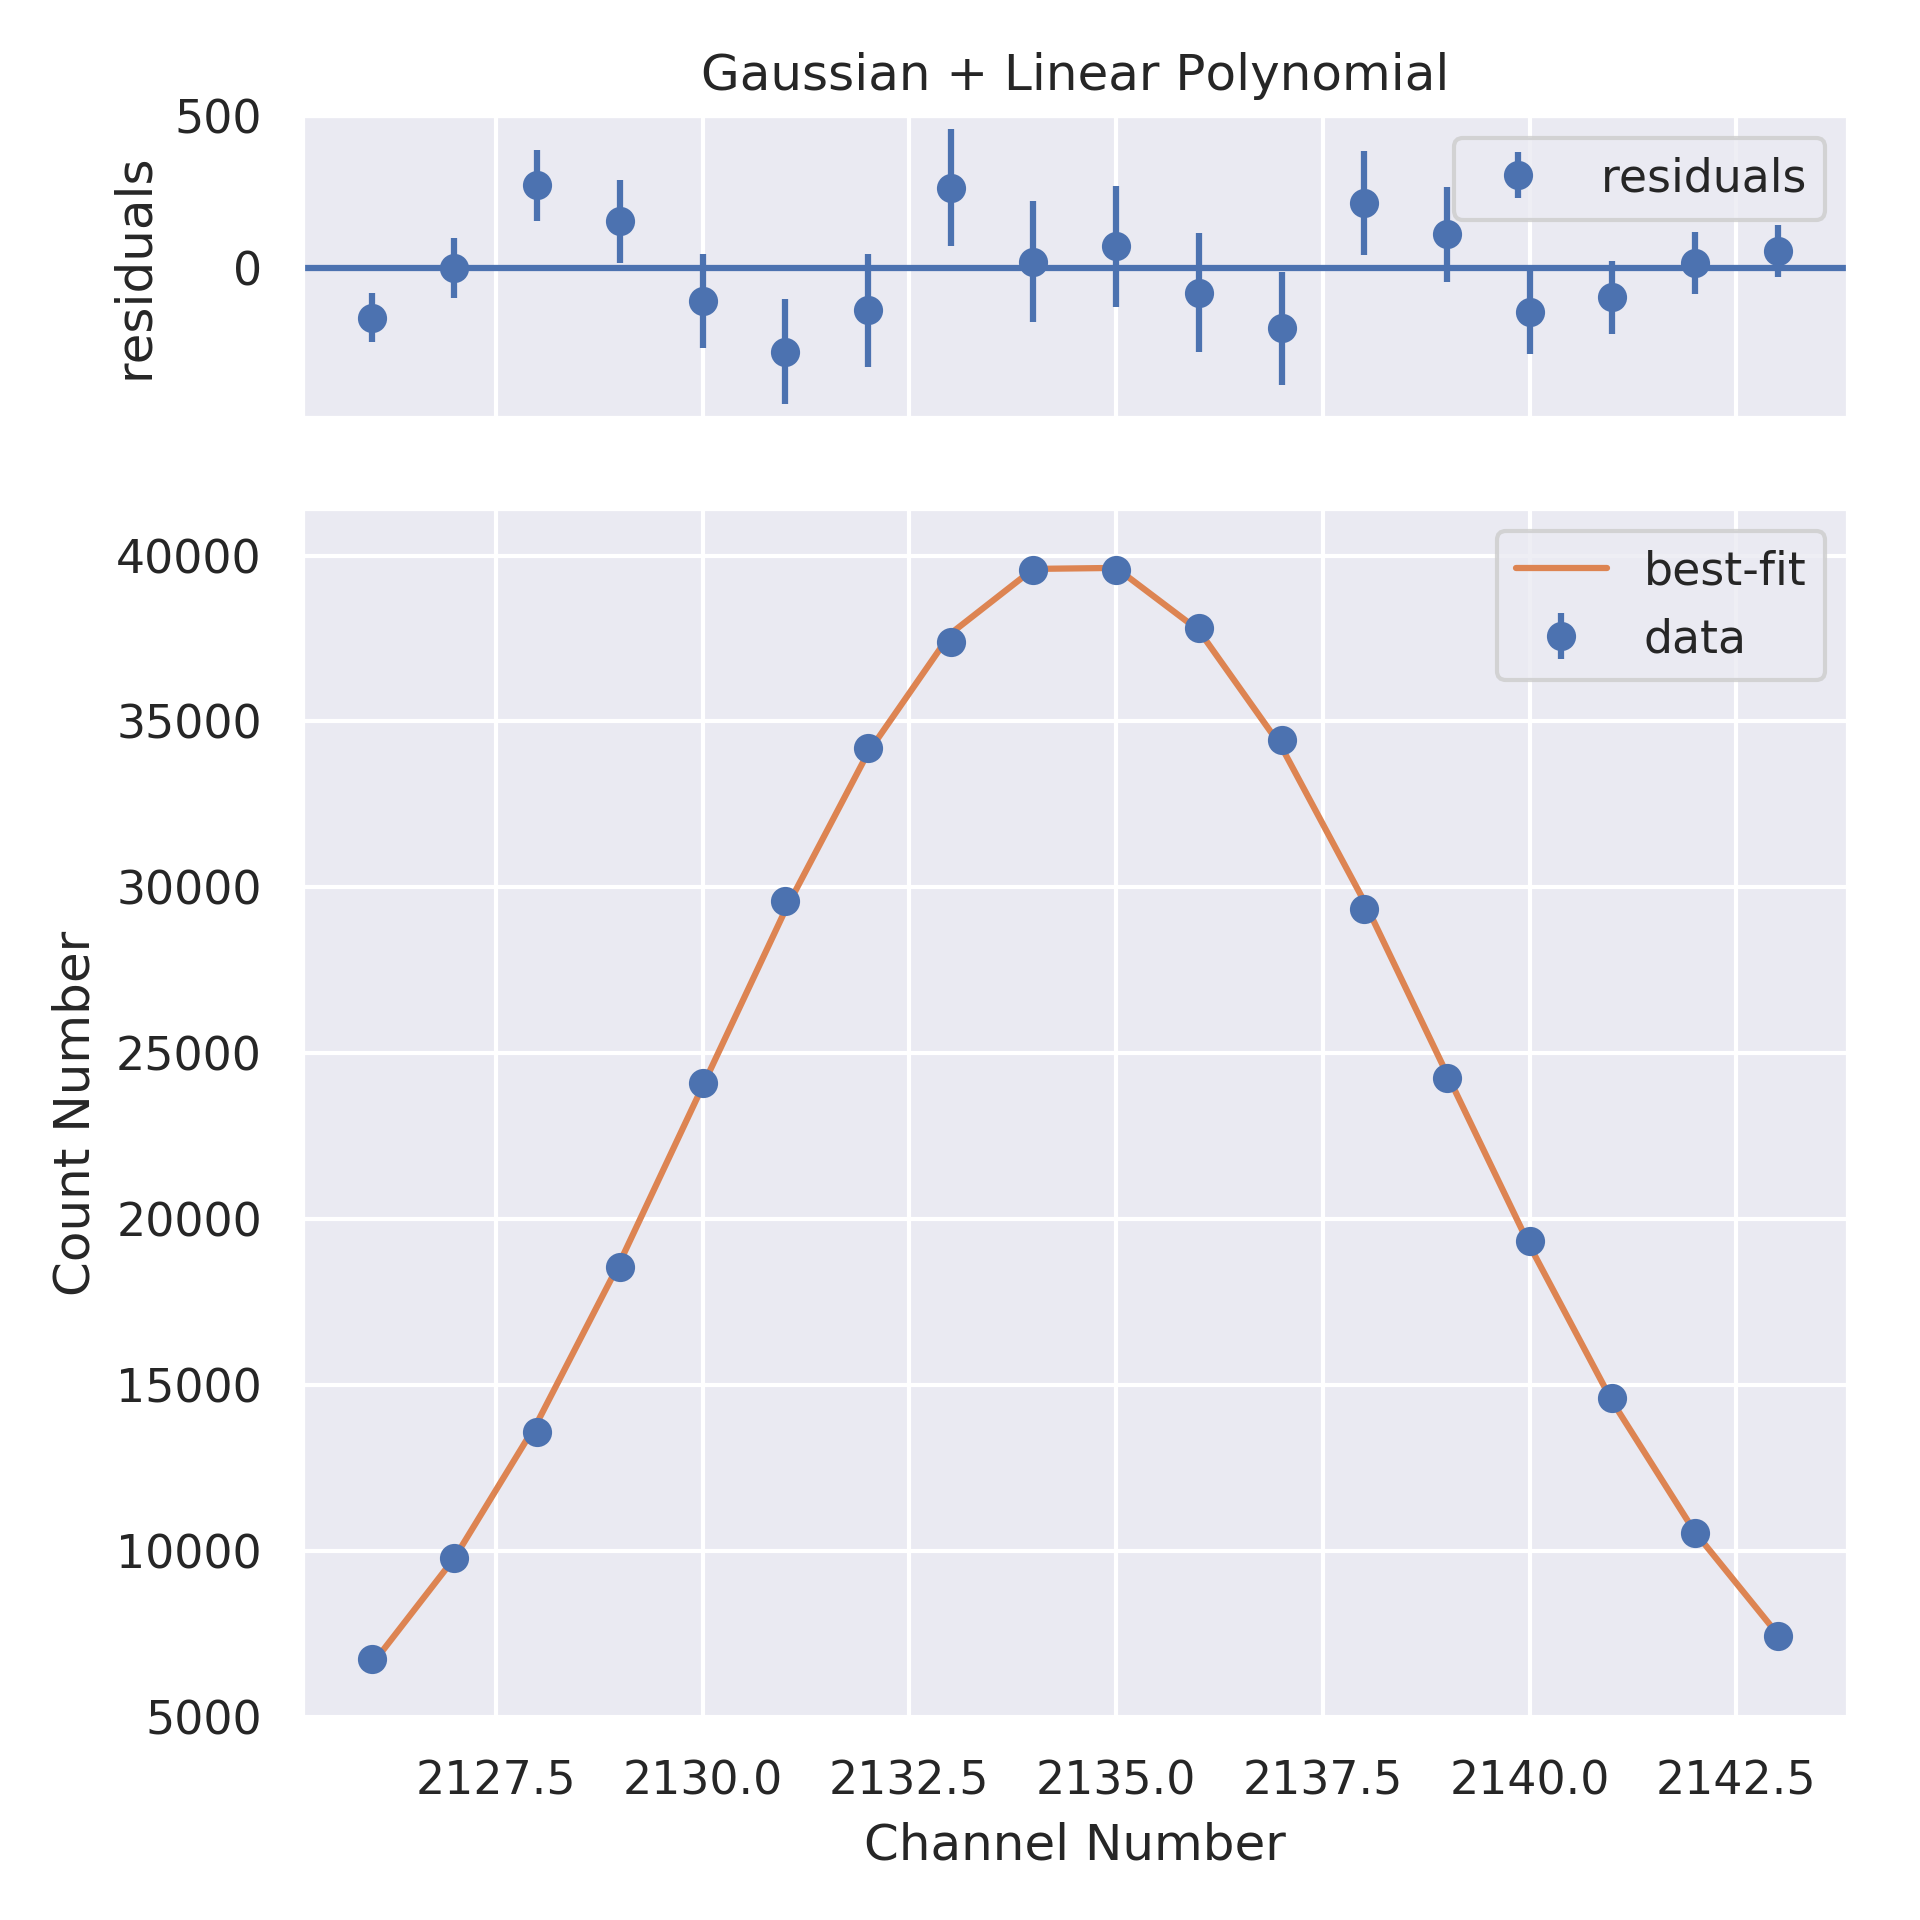
\includegraphics[width=\linewidth]{./Images/Barium133/Linear/Linear_5_Zoom.png}
    \caption{Zoomed in peak with fit}
    %\label{fig:sub2}
  \end{subfigure}
  \caption{Fit of full \& zoomed in peak of \element{Ba}{133} 303 keV peak}
  %\label{fig:test}
\end{figure}
\begin{figure}[H]
  \centering
  \begin{subfigure}{.5\linewidth}
    \centering
    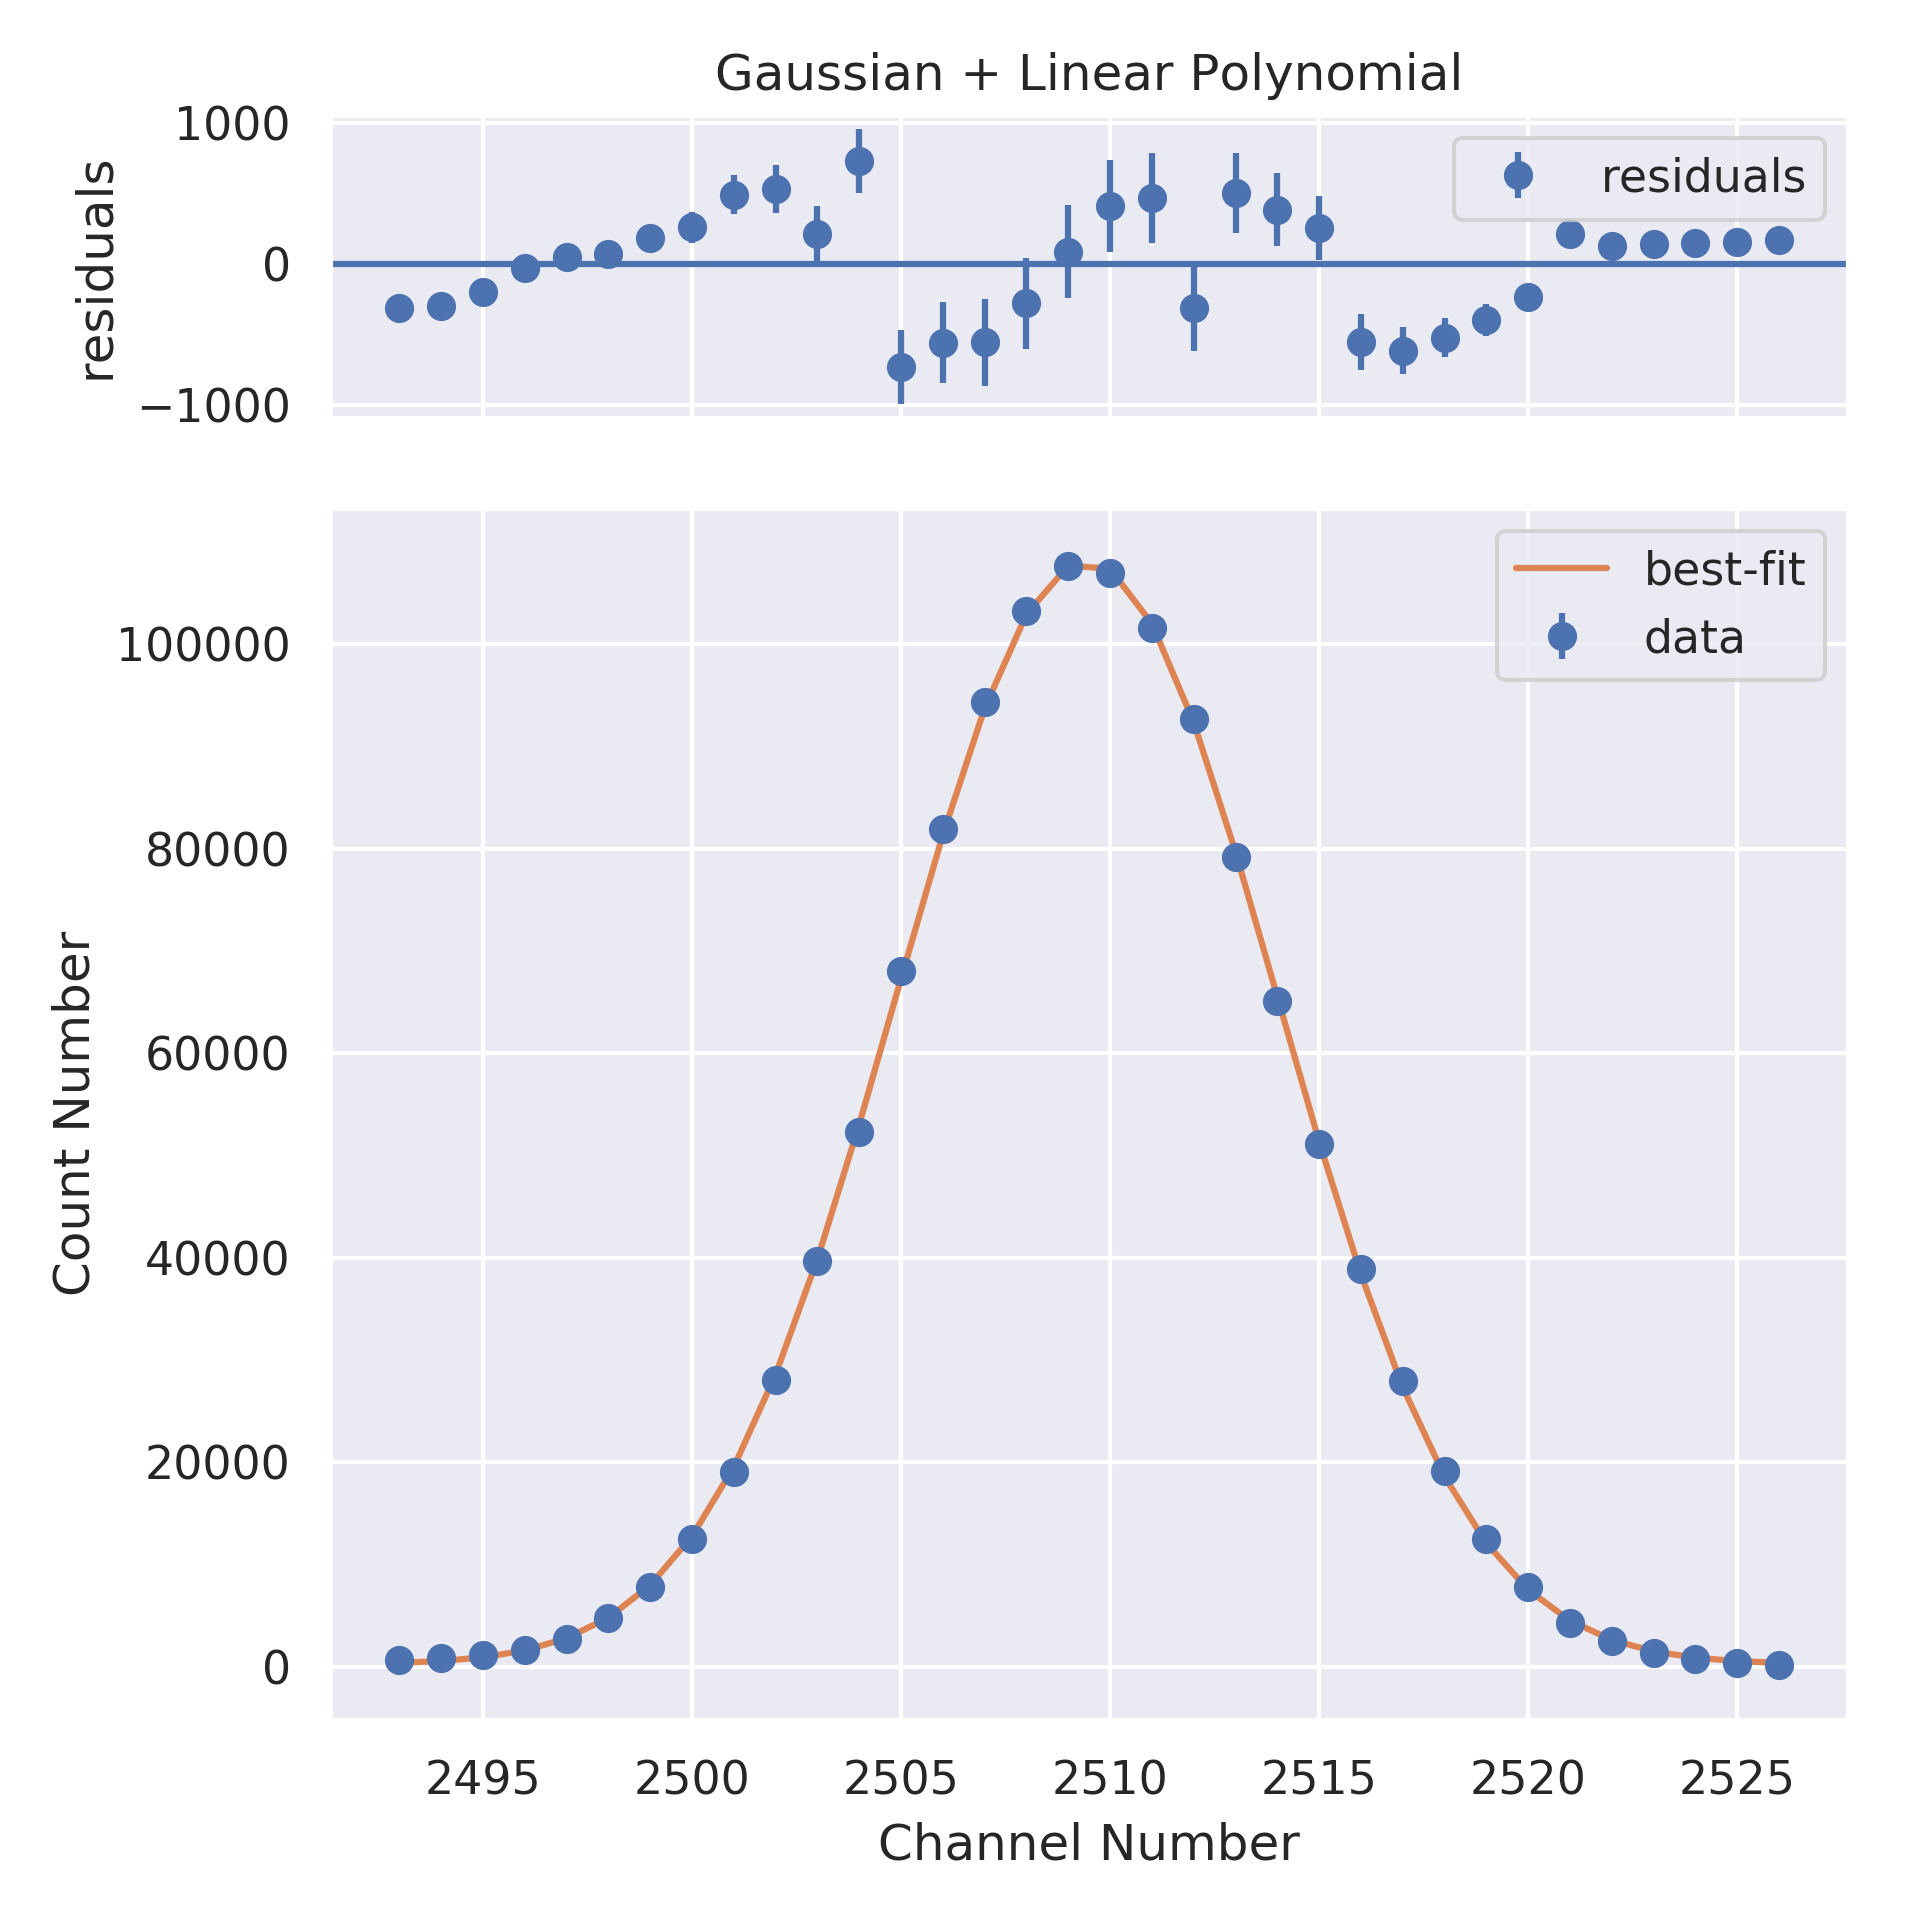
\includegraphics[width=\linewidth]{./Images/Barium133/Linear/Linear_6_Full.png}
    \caption{Full peak with fit}
    %\label{fig:sub1}
  \end{subfigure}%
  \begin{subfigure}{.5\linewidth}
    \centering
    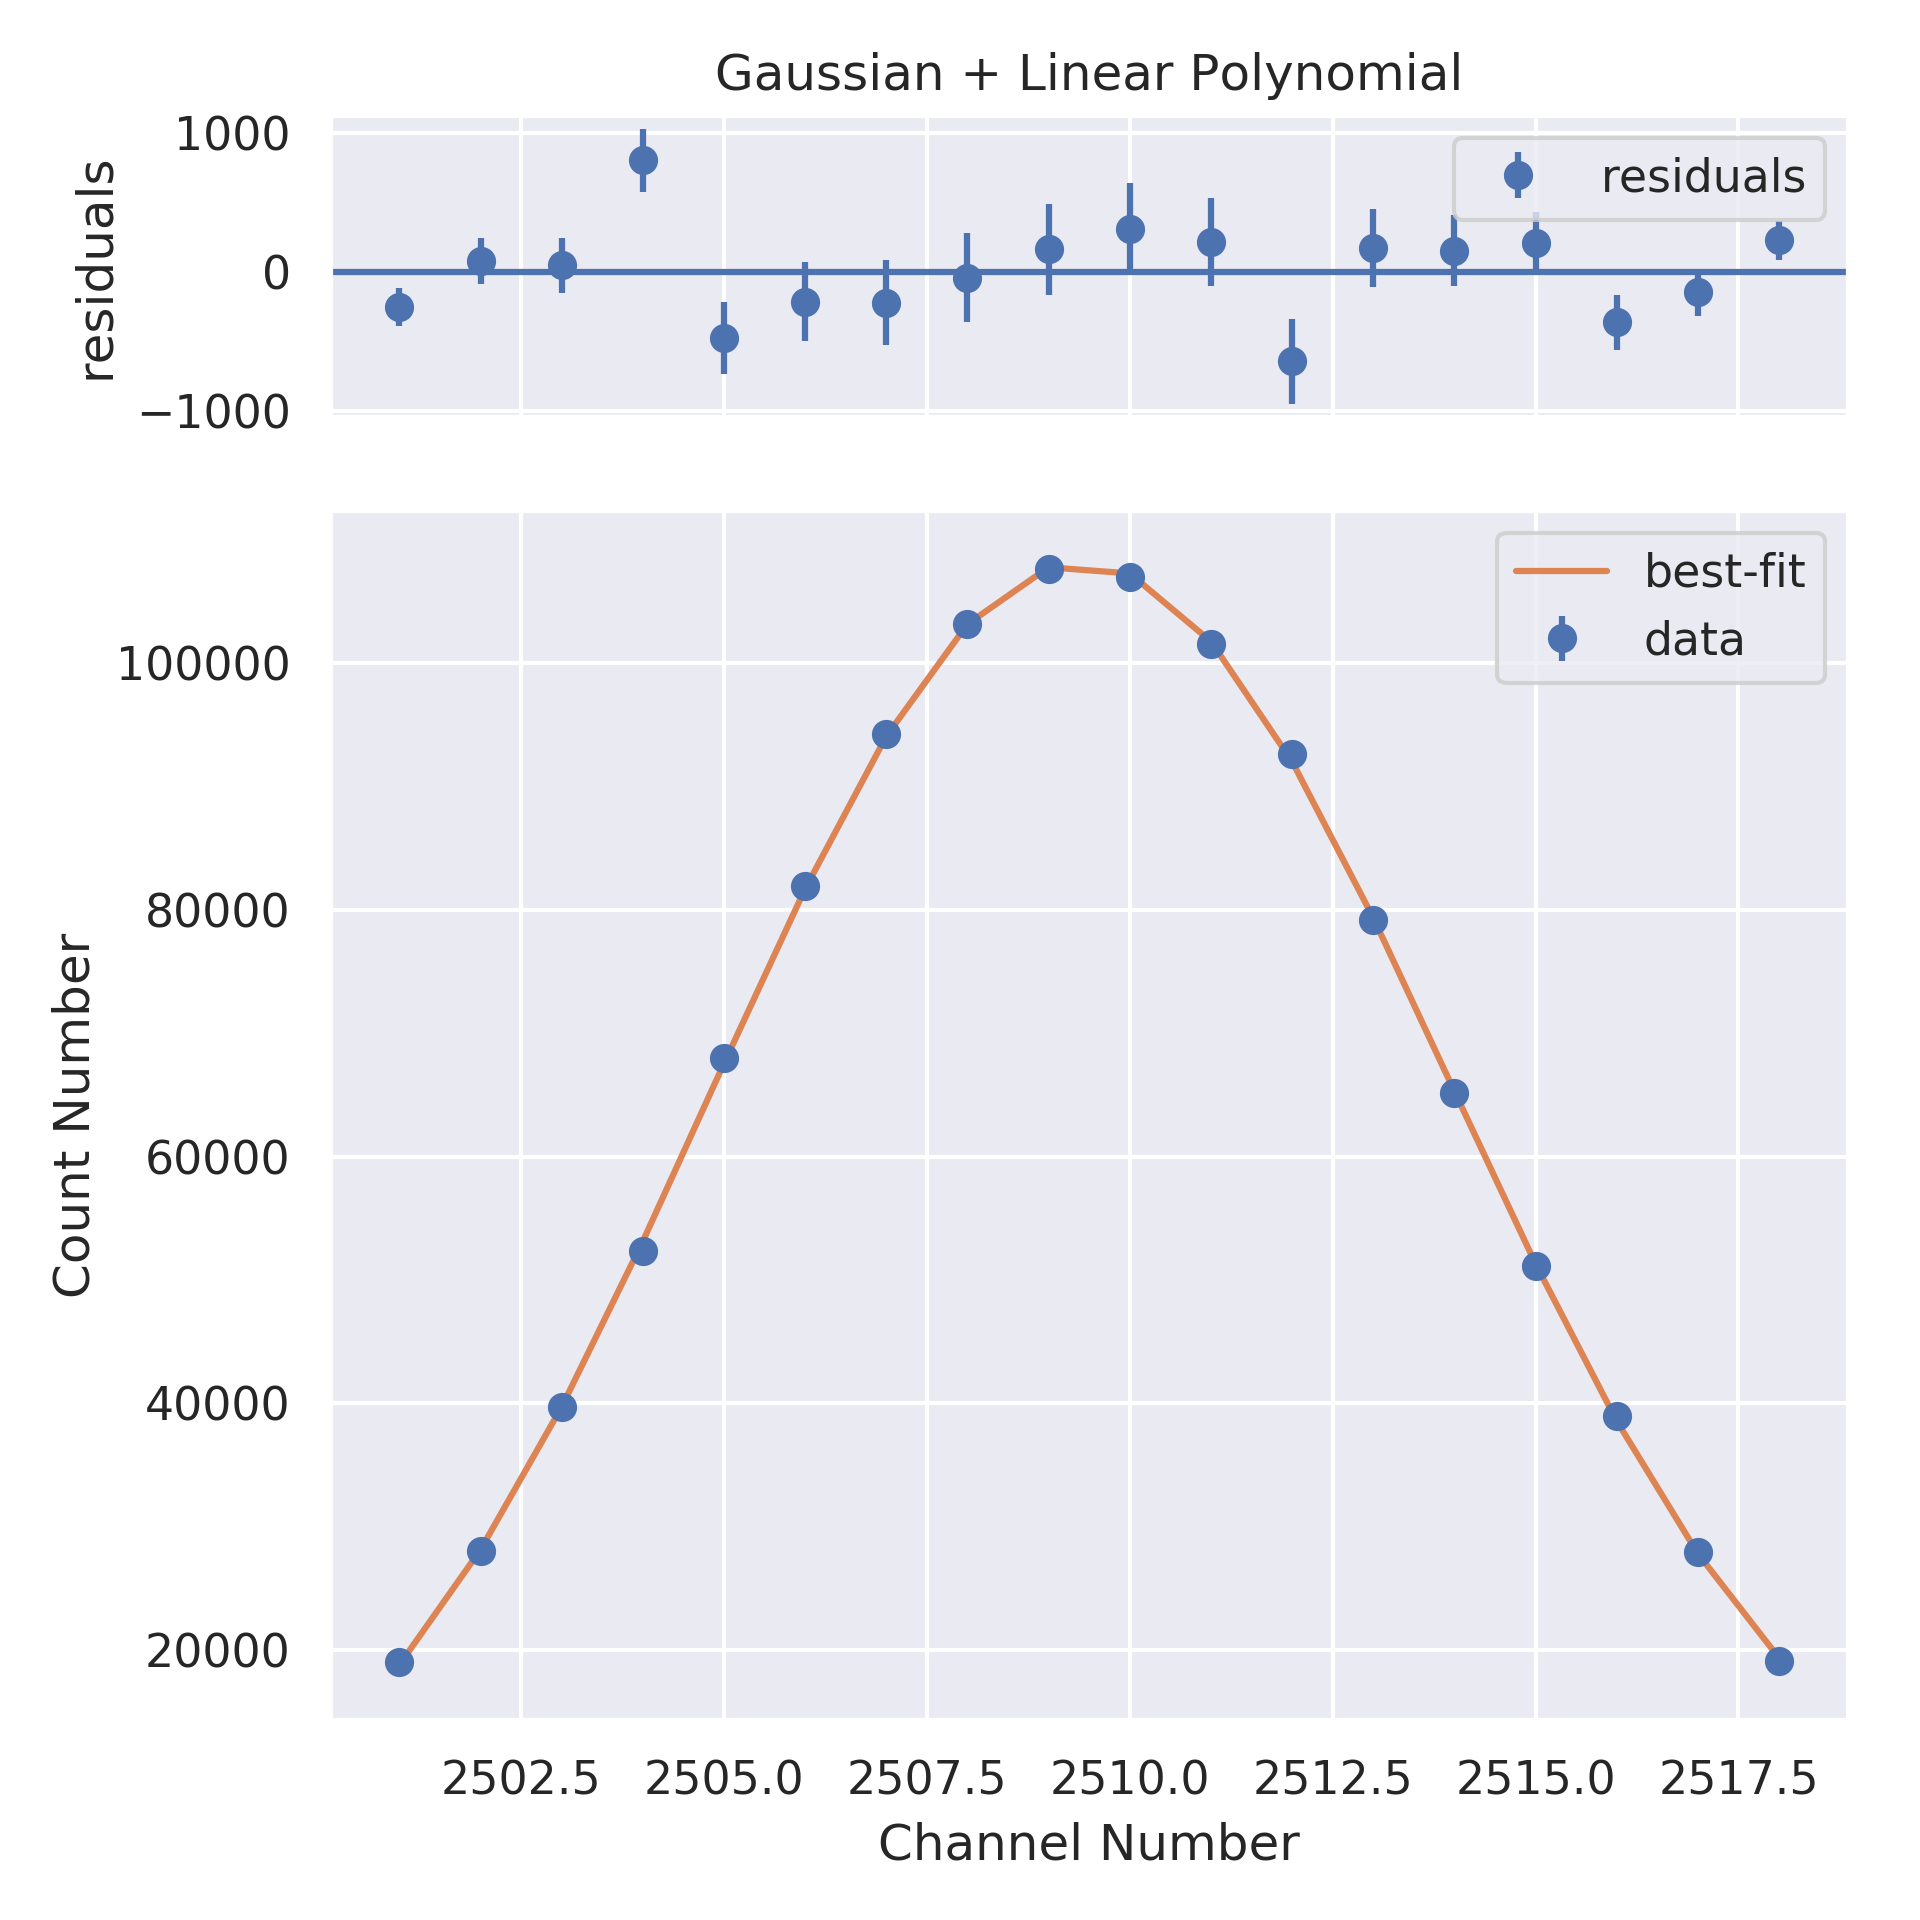
\includegraphics[width=\linewidth]{./Images/Barium133/Linear/Linear_6_Zoom.png}
    \caption{Zoomed in peak with fit}
    %\label{fig:sub2}
  \end{subfigure}
  \caption{Fit of full \& zoomed in peak of \element{Ba}{133} 356 keV peak}
  %\label{fig:test}
\end{figure}
\begin{figure}[H]
  \centering
  \begin{subfigure}{.5\linewidth}
    \centering
    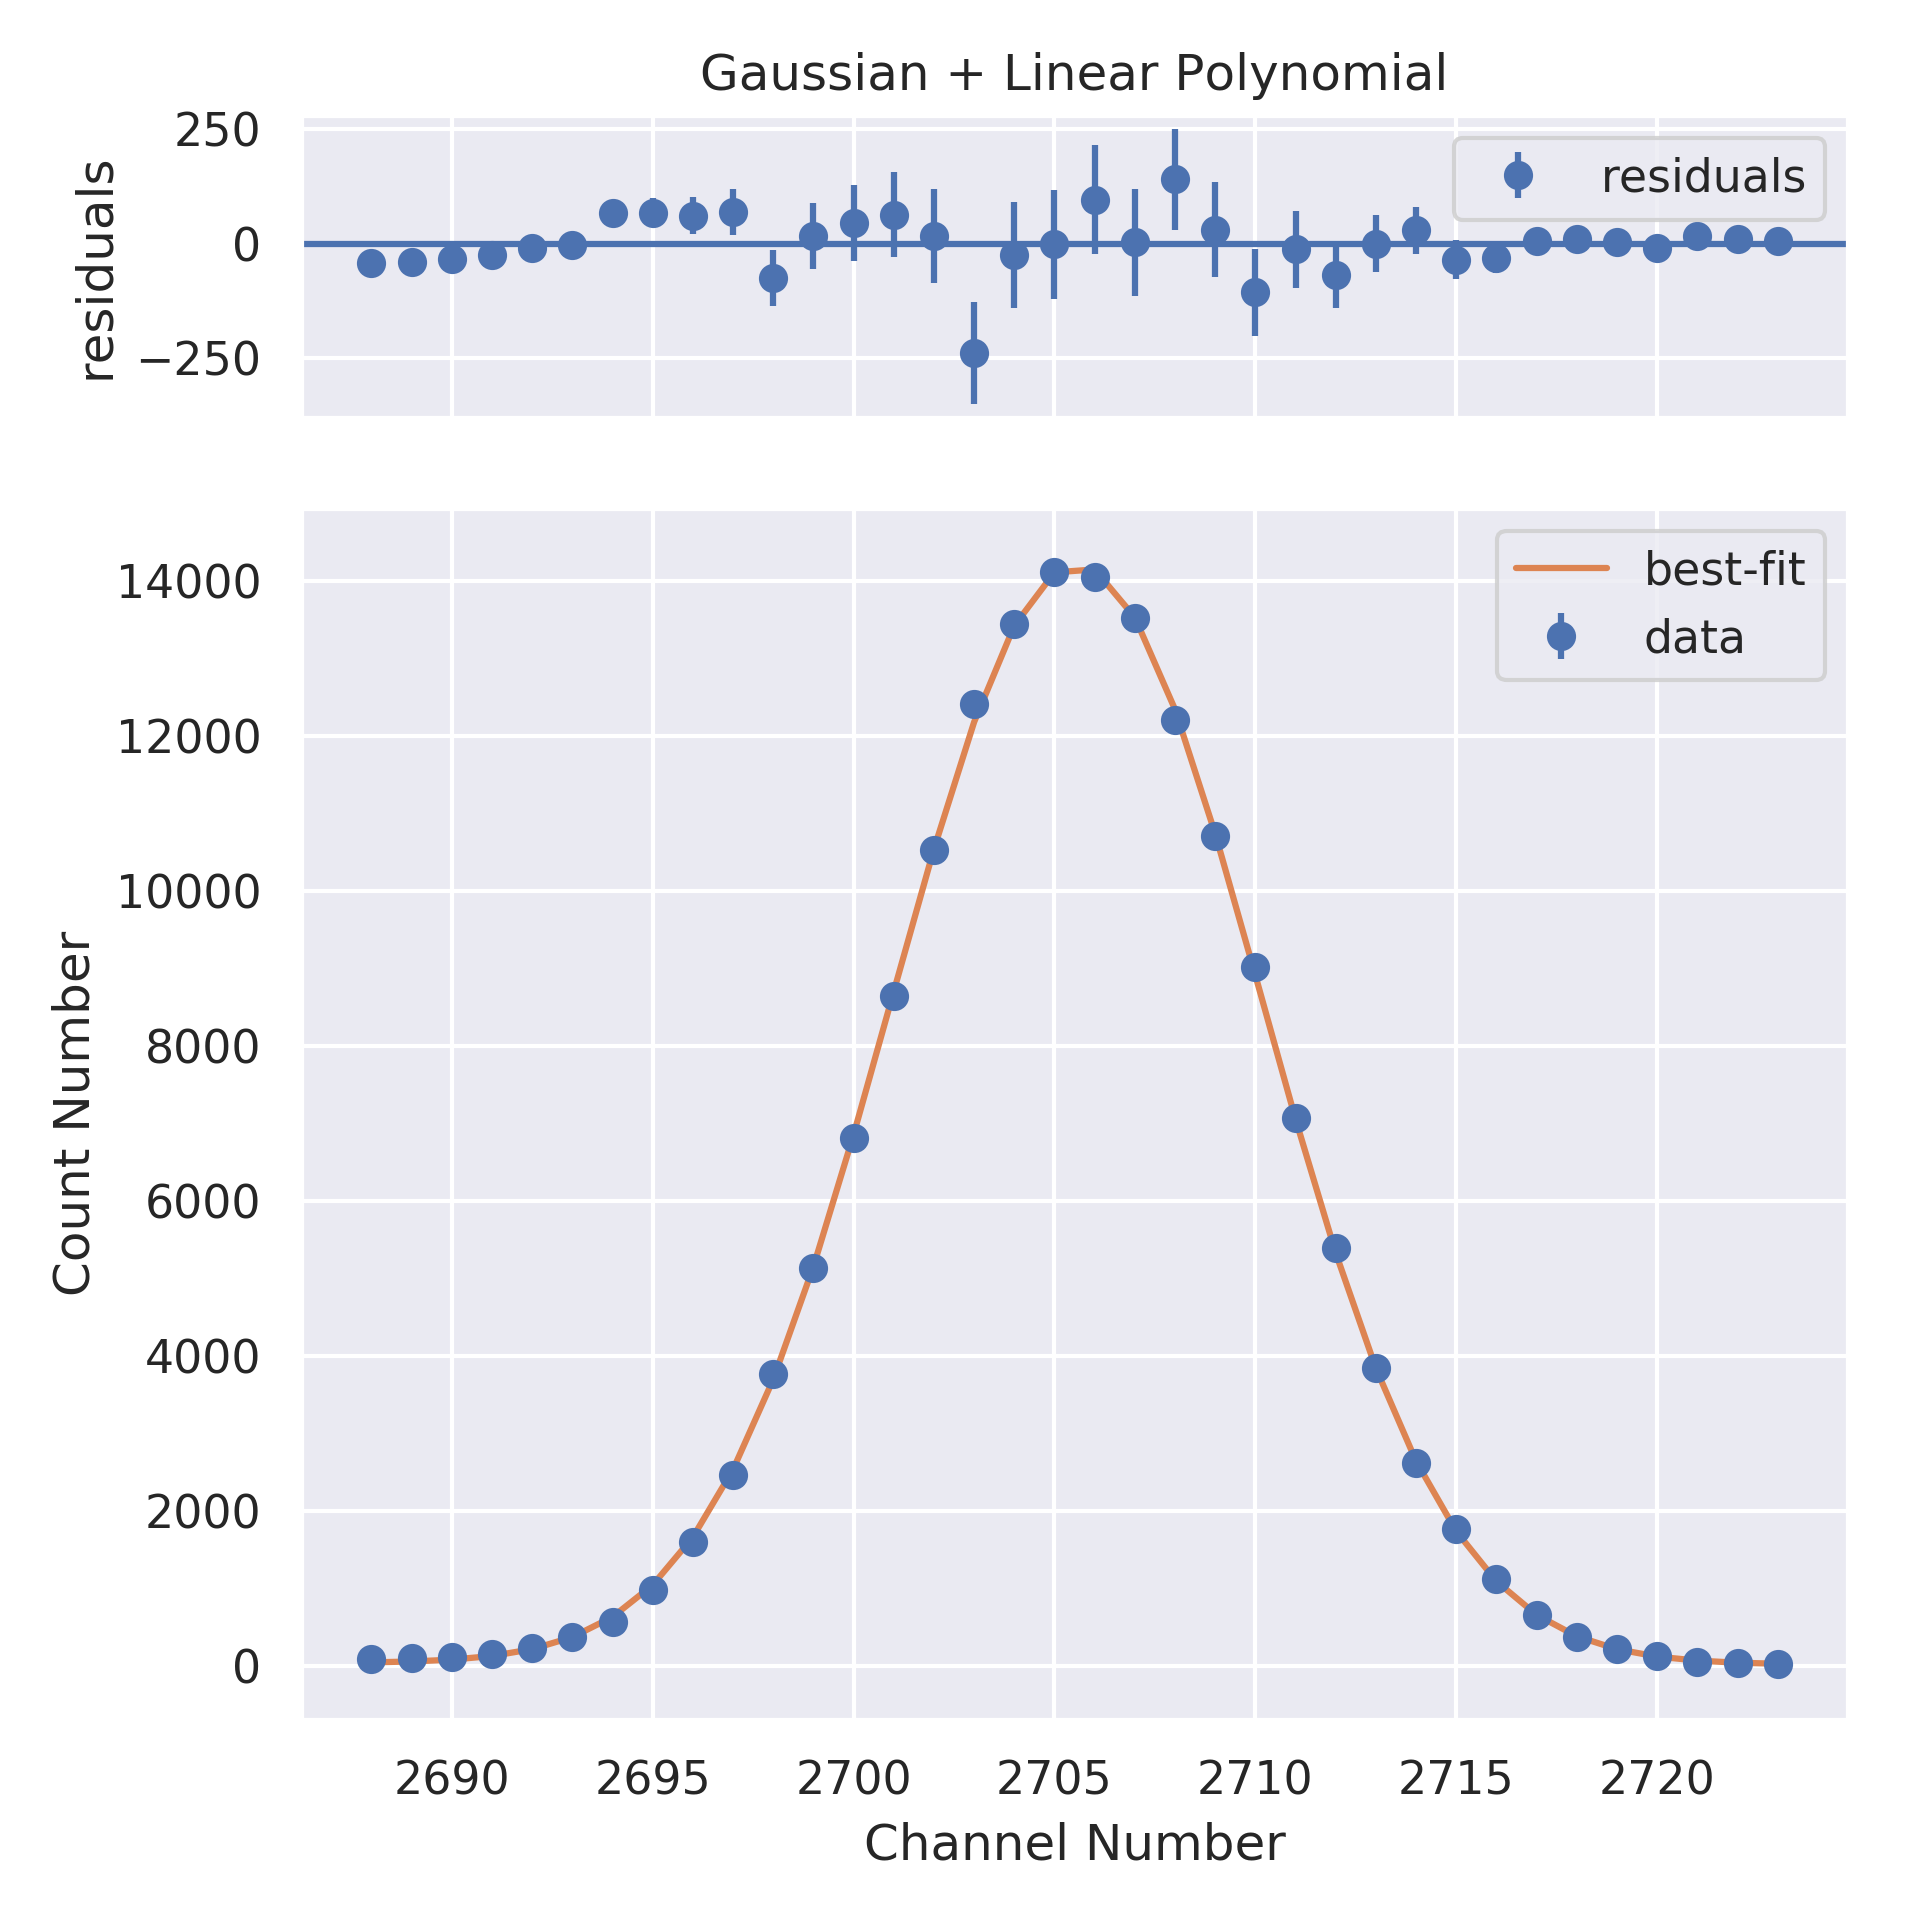
\includegraphics[width=\linewidth]{./Images/Barium133/Linear/Linear_7_Full.png}
    \caption{Full peak with fit}
    %\label{fig:sub1}
  \end{subfigure}%
  \begin{subfigure}{.5\linewidth}
    \centering
    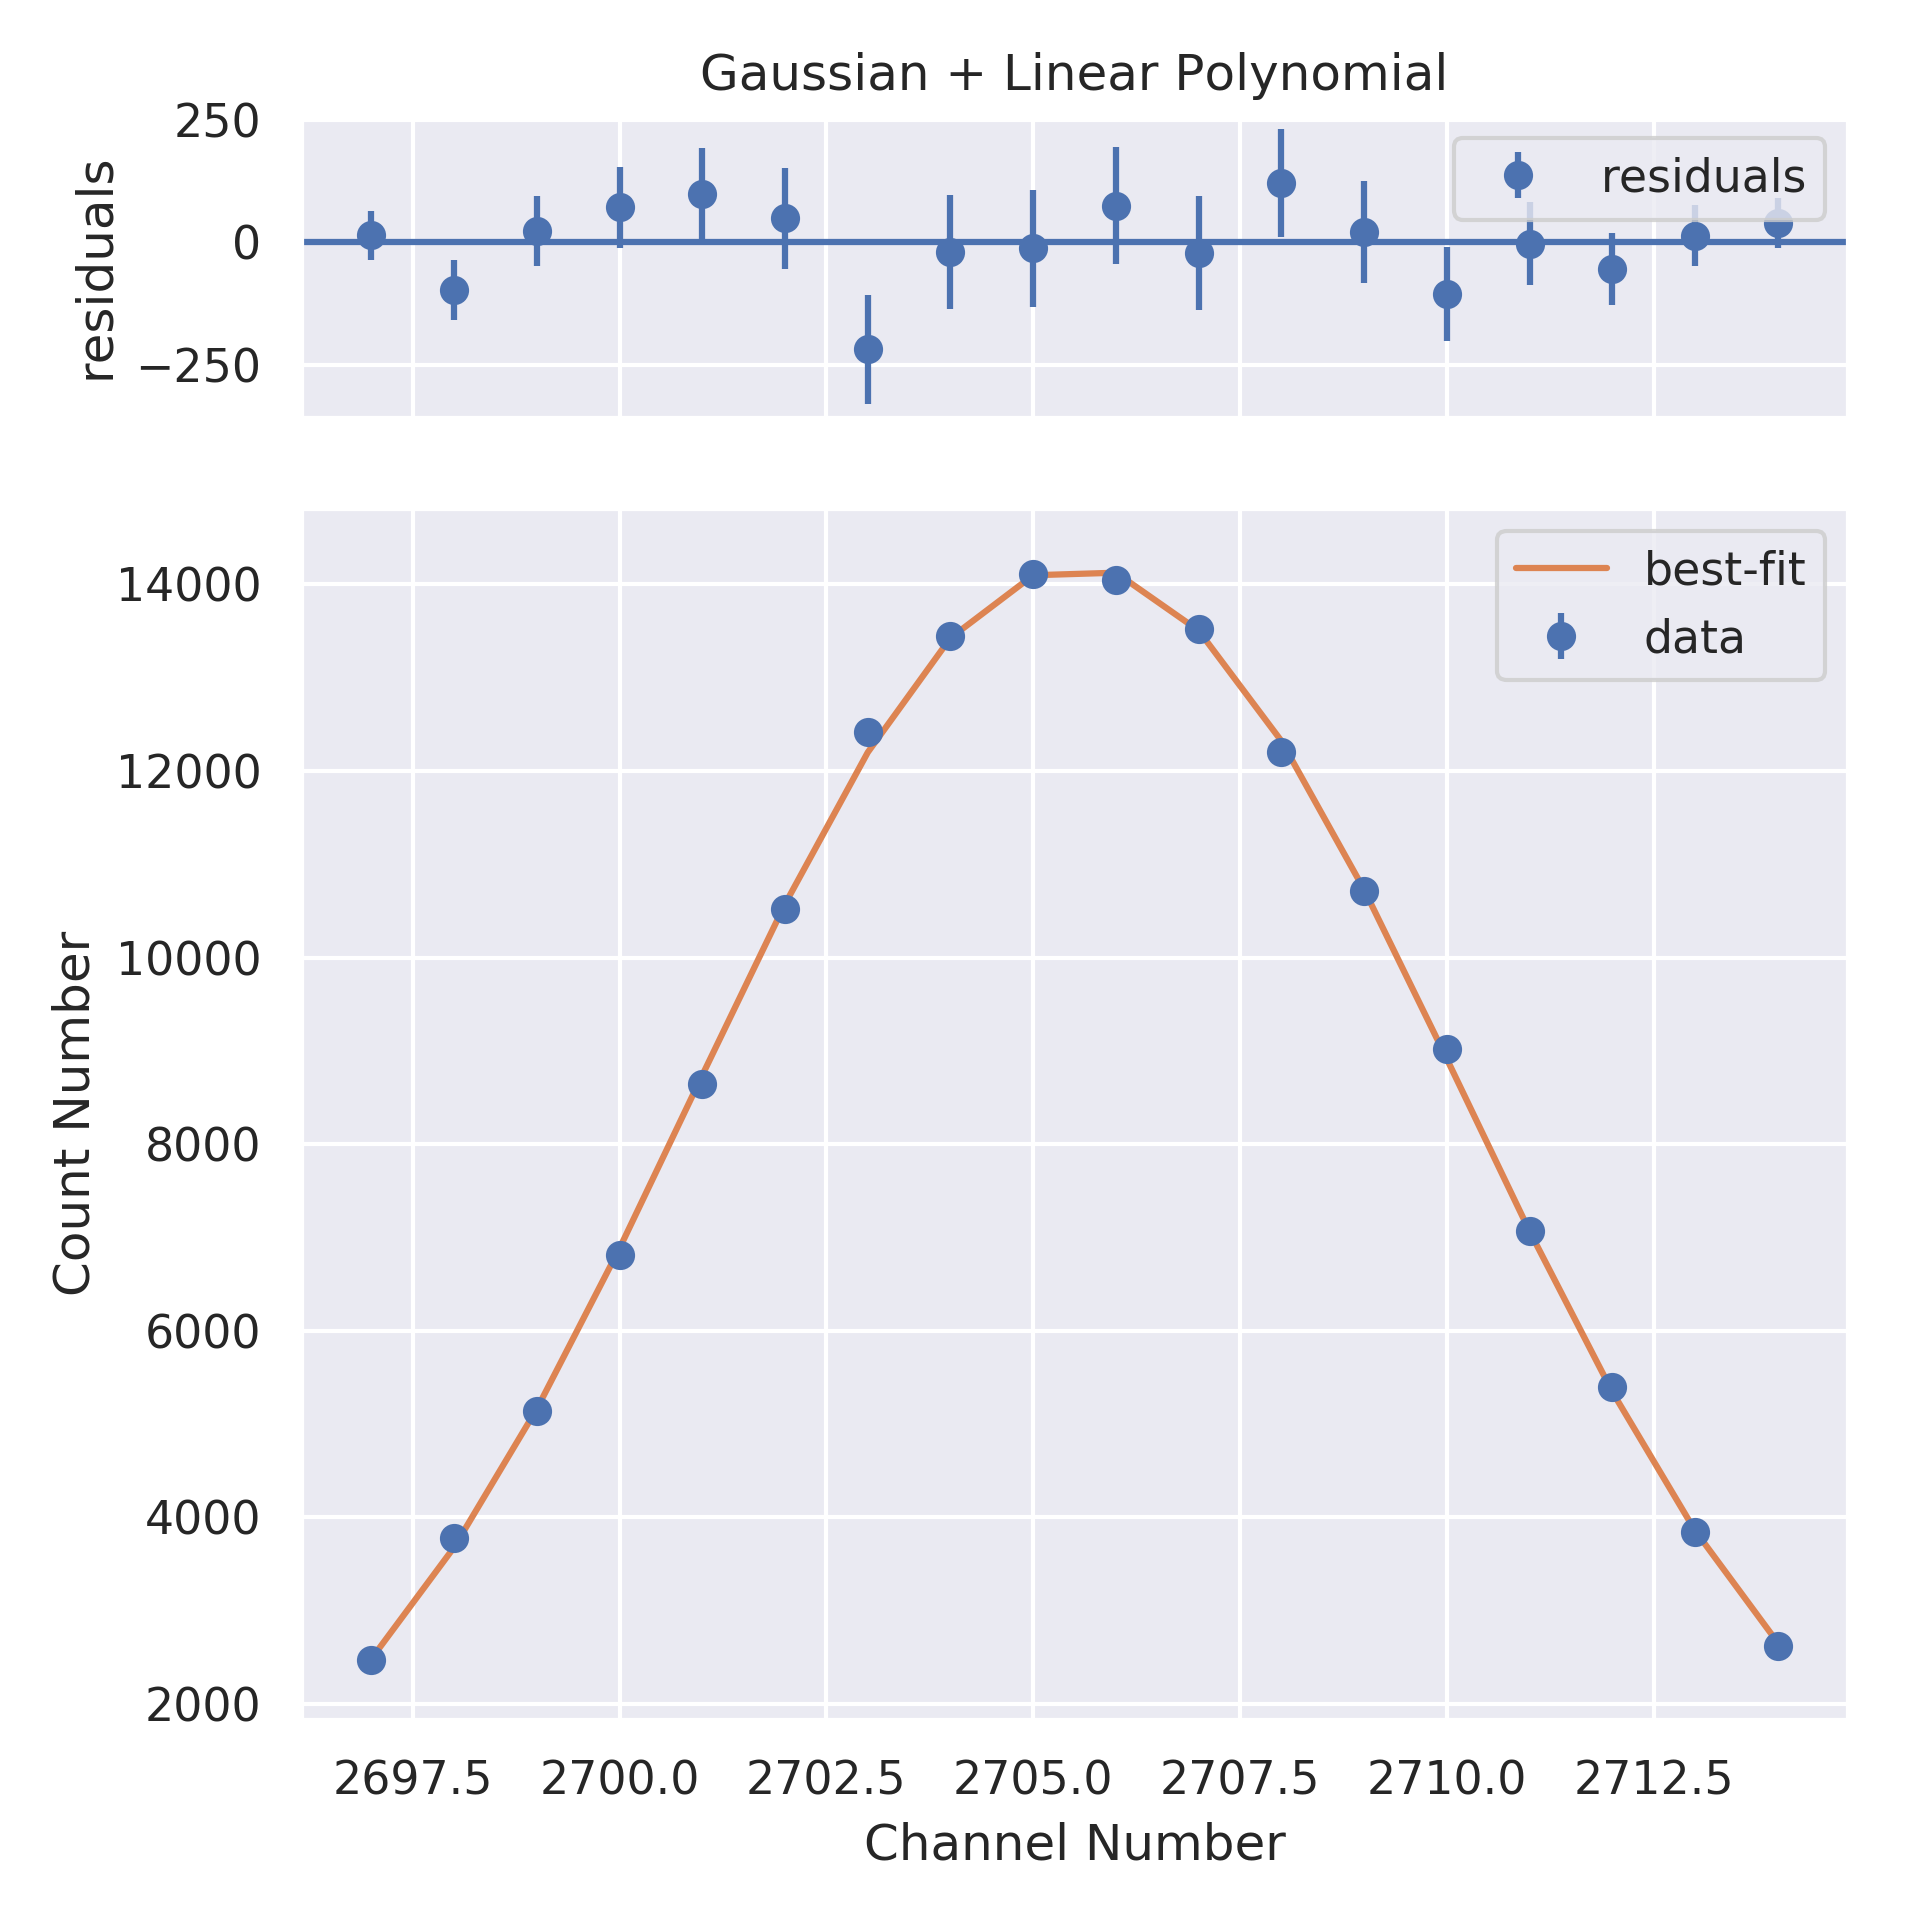
\includegraphics[width=\linewidth]{./Images/Barium133/Linear/Linear_7_Zoom.png}
    \caption{Zoomed in peak with fit}
    %\label{fig:sub2}
  \end{subfigure}
  \caption{Fit of full \& zoomed in peak of \element{Ba}{133} 384 keV peak}
  %\label{fig:test}
\end{figure}
\clearpage
\subsubsection{Quadratic + Gaussian Fit}
\begin{figure}[H]
  \centering
  \begin{subfigure}{.5\linewidth}
    \centering
    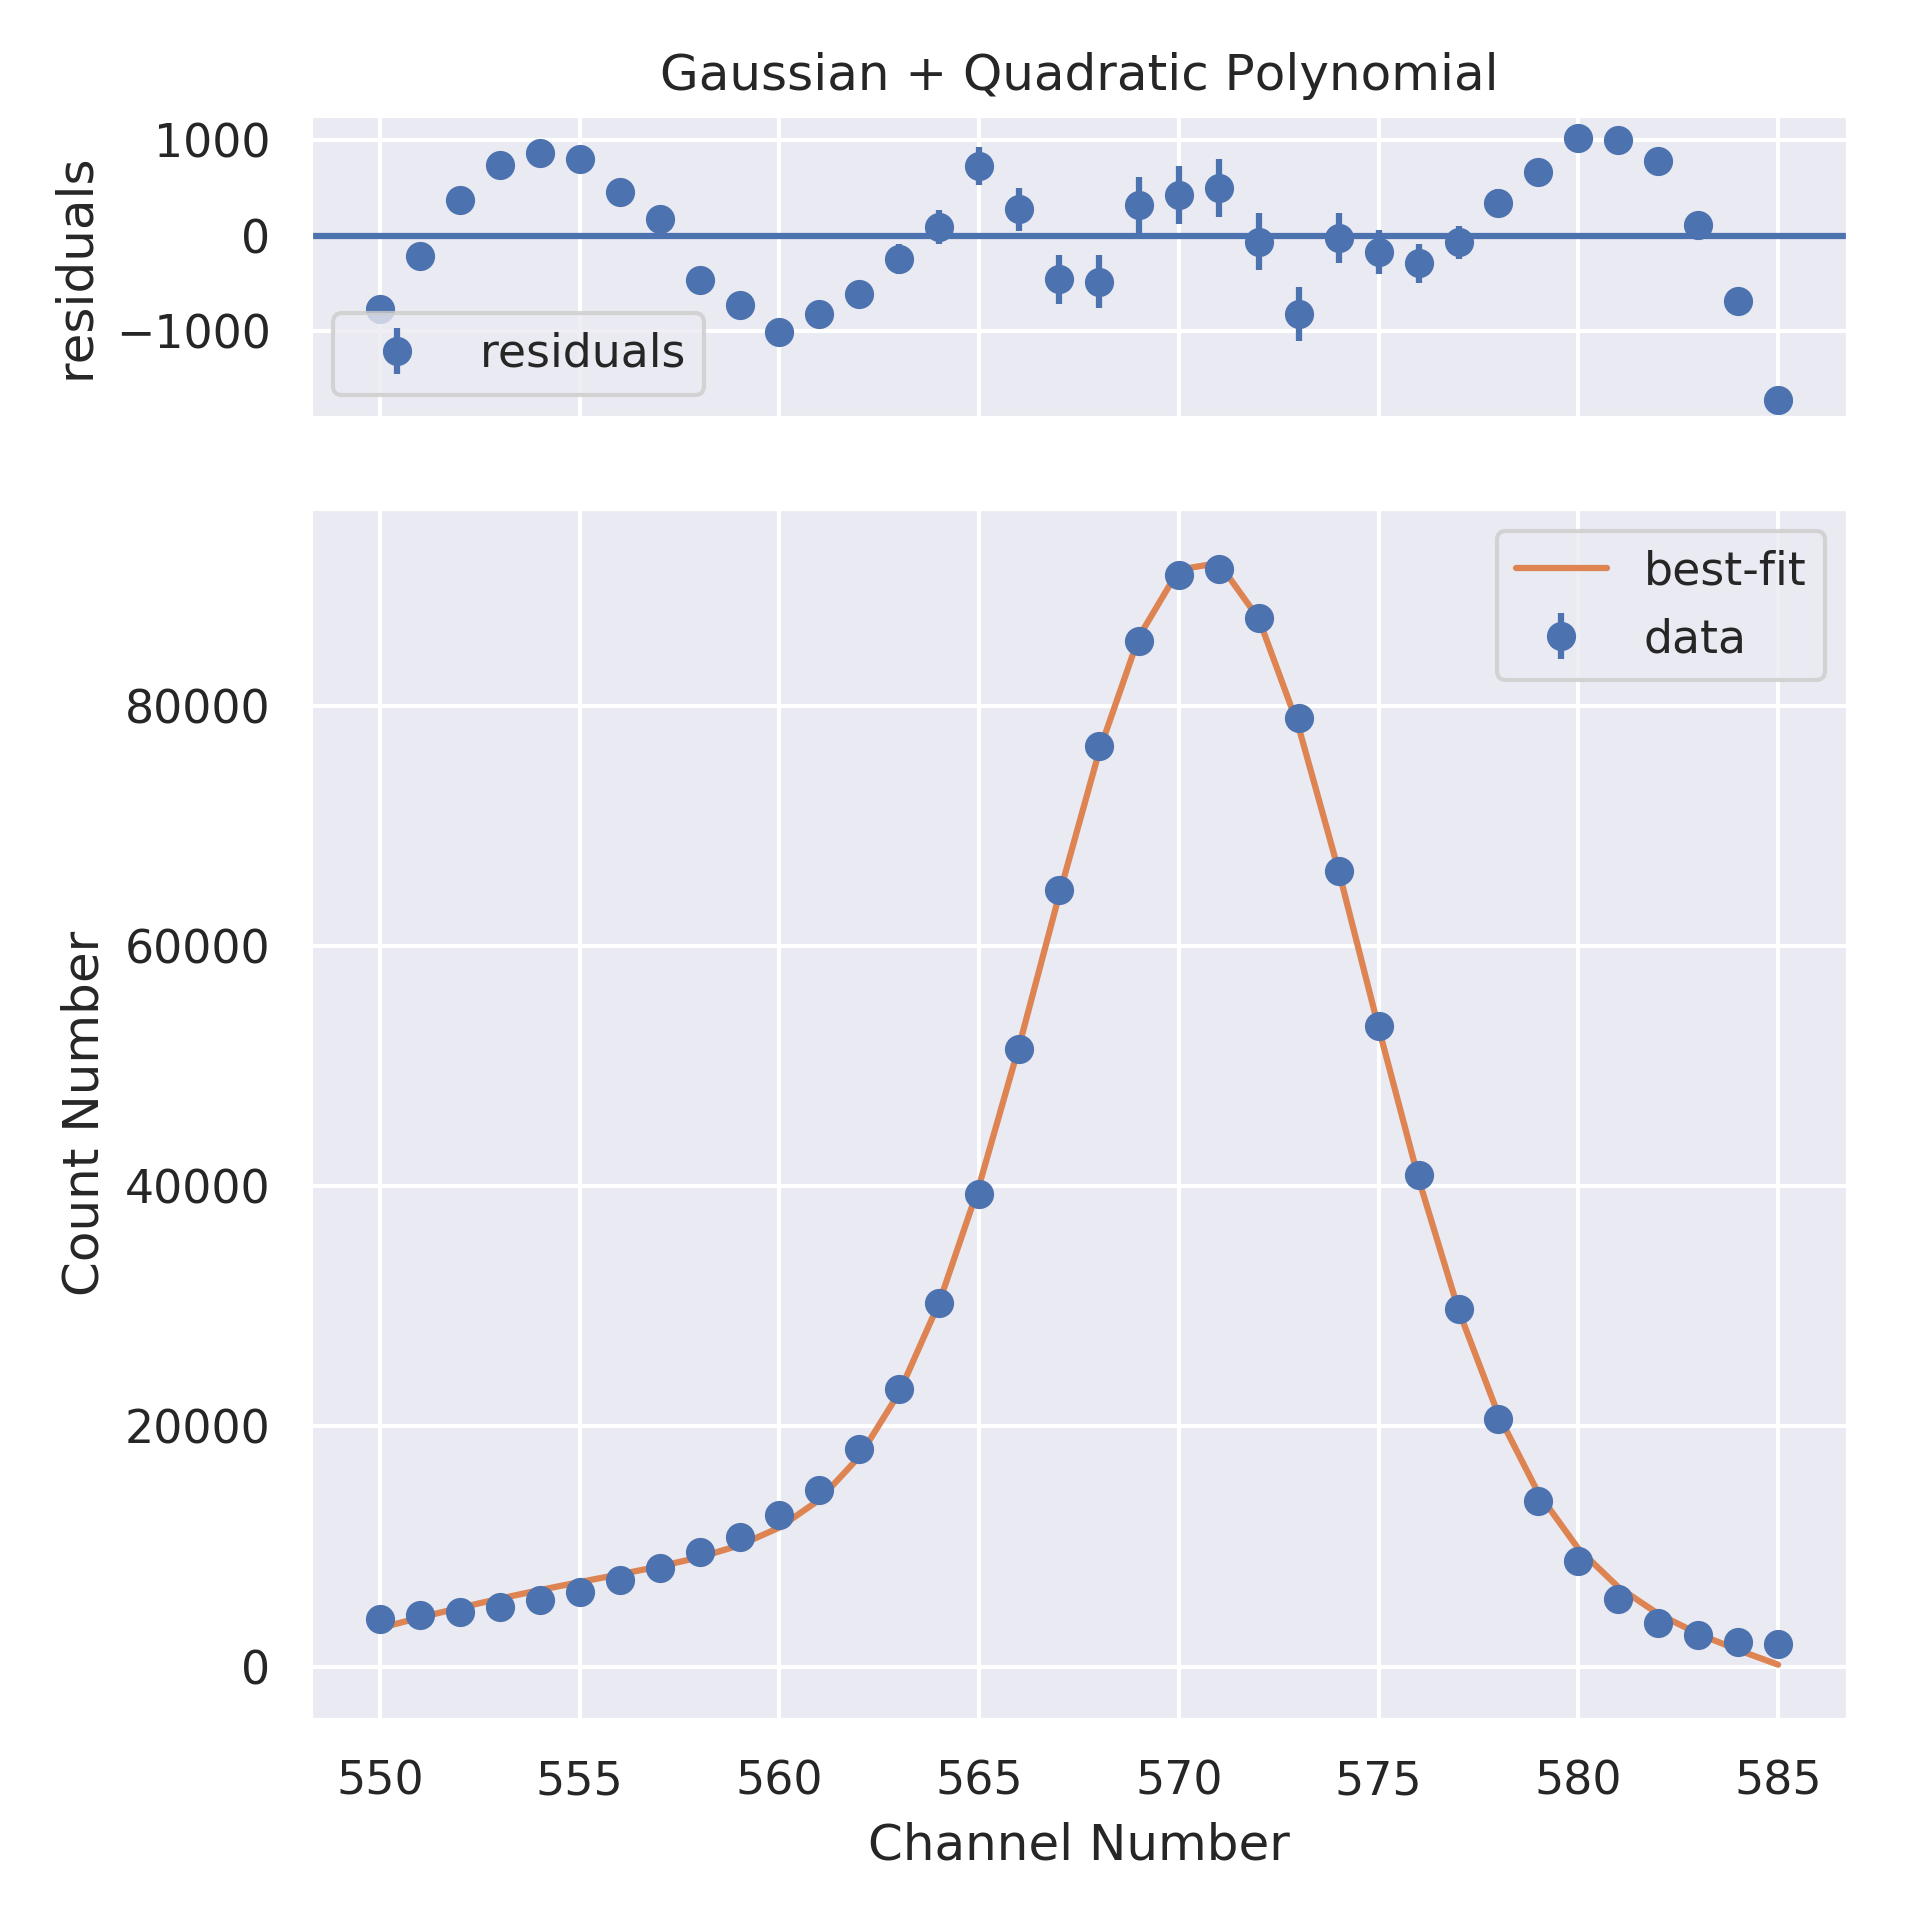
\includegraphics[width=\linewidth]{./Images/Barium133/Quad/Quad_1_Full.png}
    \caption{Full peak with fit}
    %\label{fig:sub1}
  \end{subfigure}%
  \begin{subfigure}{.5\linewidth}
    \centering
    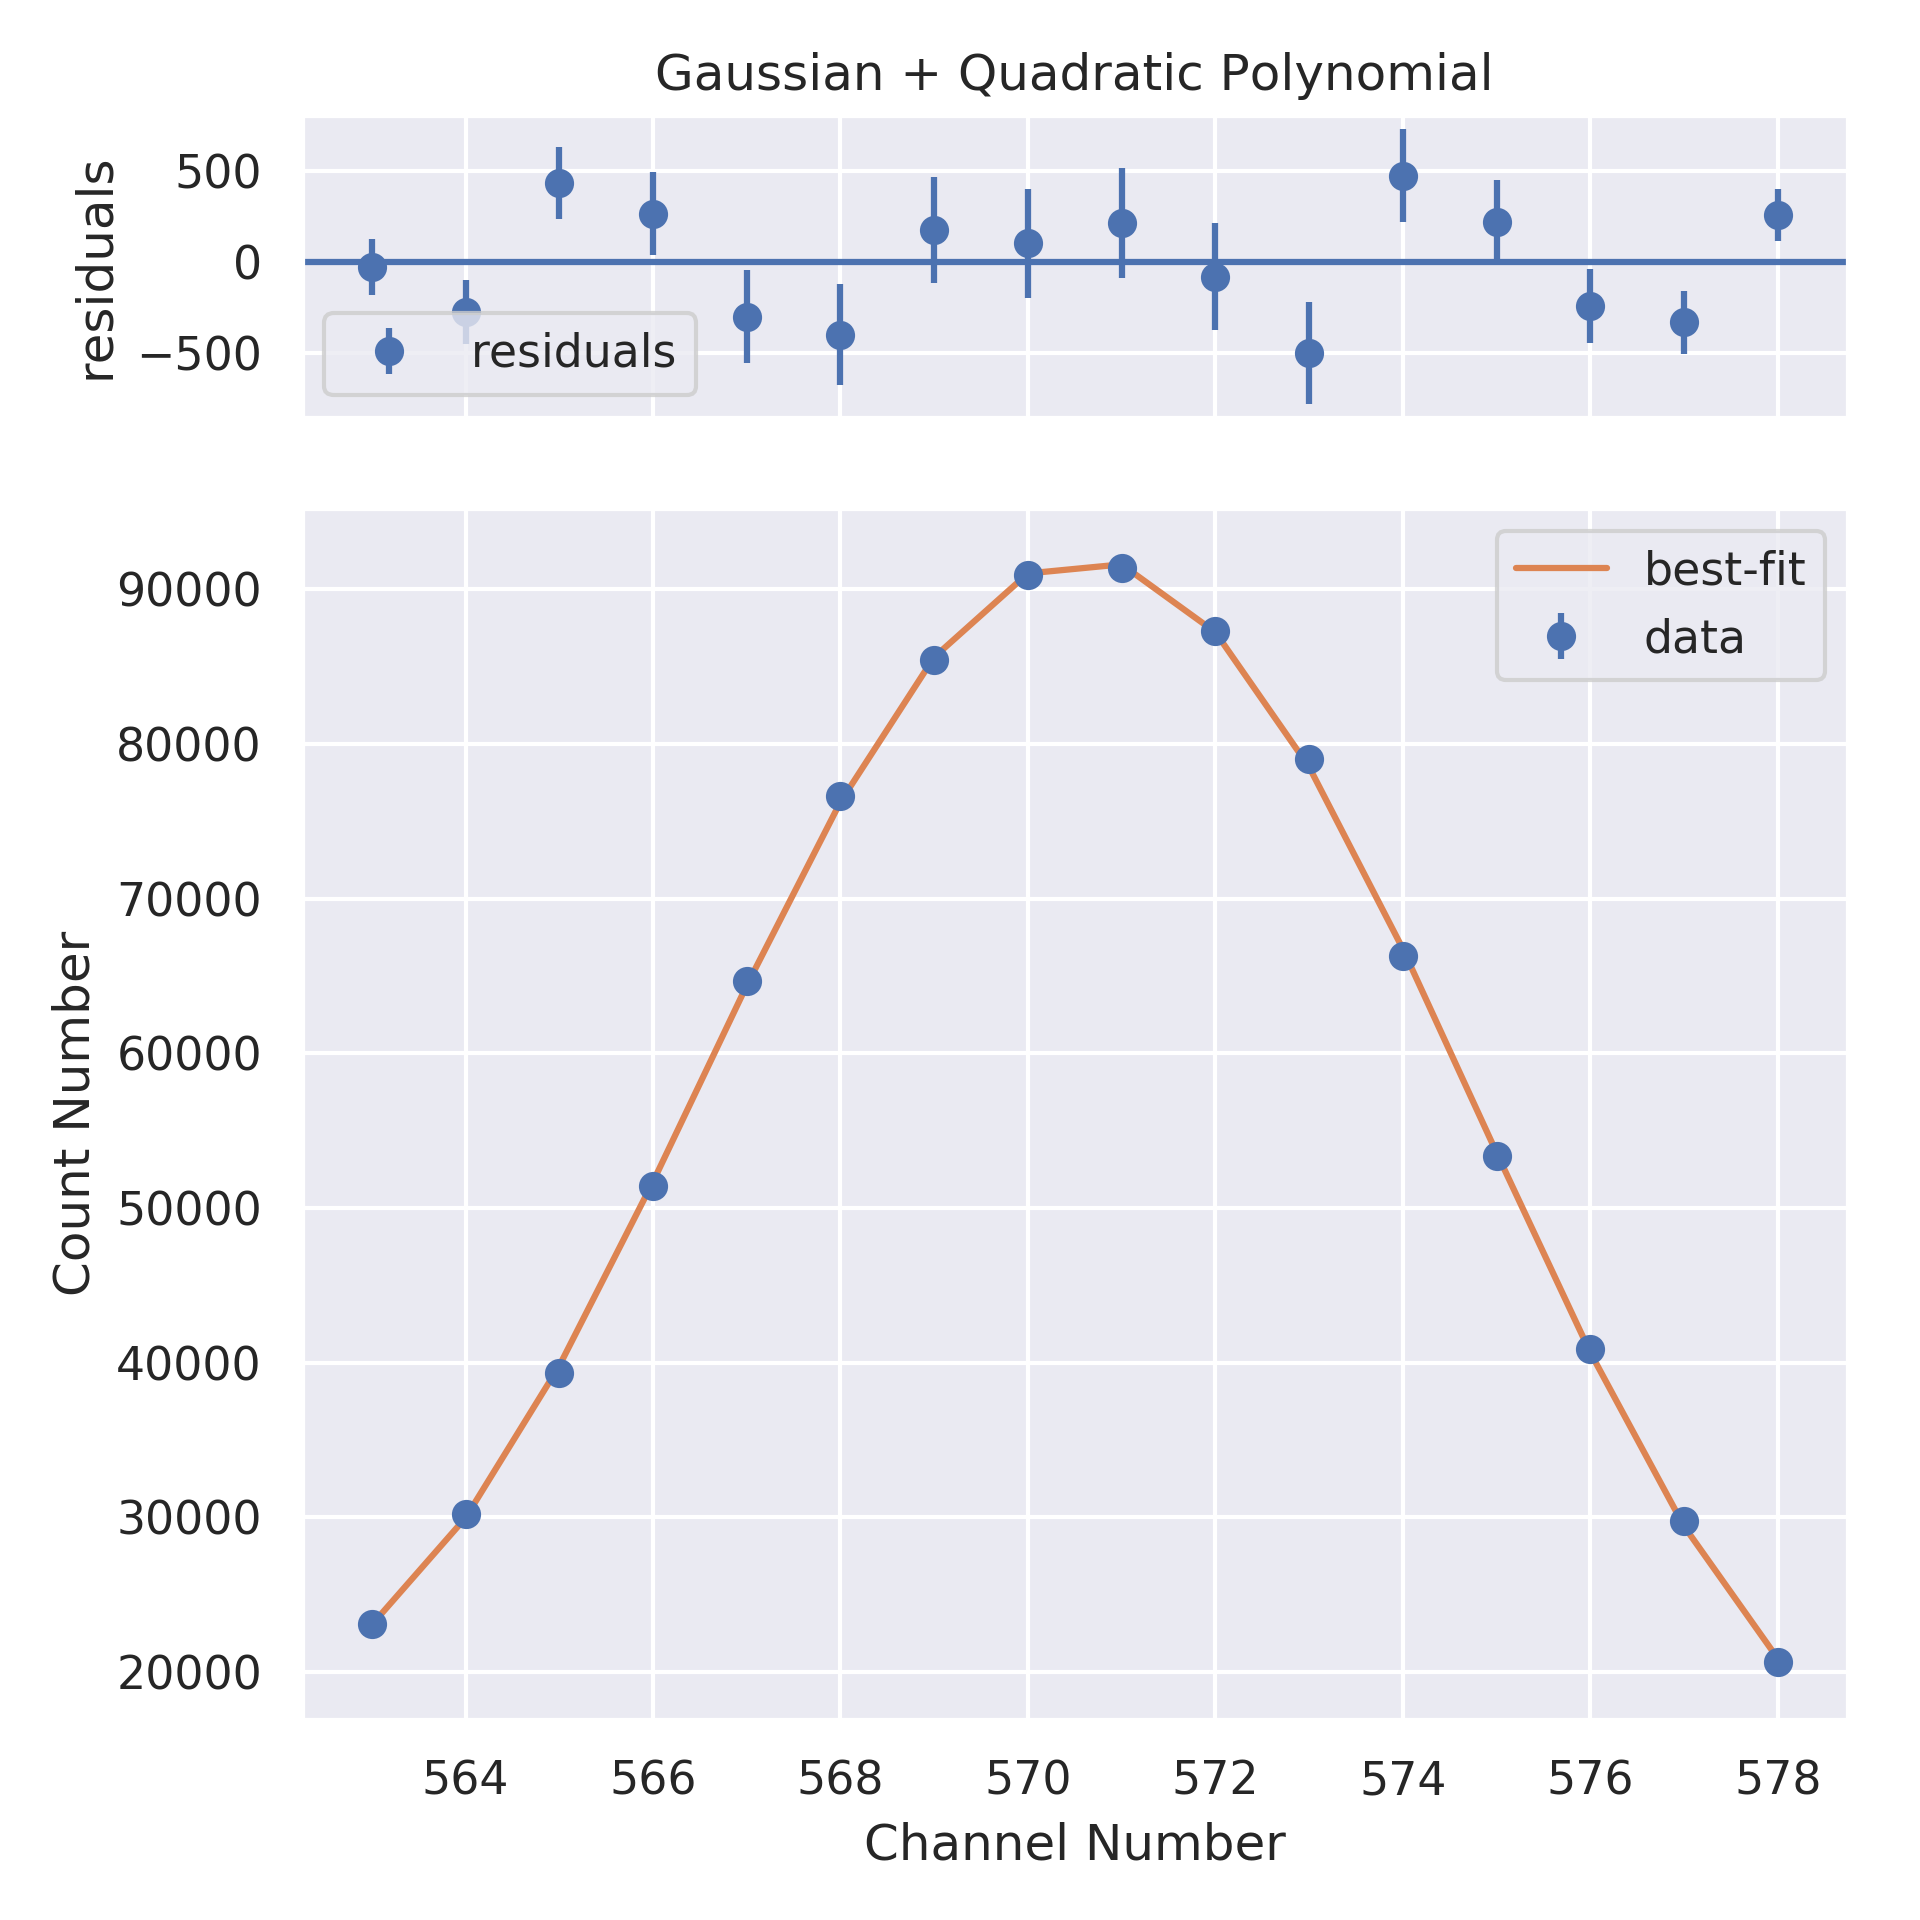
\includegraphics[width=\linewidth]{./Images/Barium133/Quad/Quad_1_Zoom.png}
    \caption{Zoomed in peak with fit}
    %\label{fig:sub2}
  \end{subfigure}
  \caption{Fit of full \& zoomed in peak of \element{Ba}{133} 81 keV peak}
  %\label{fig:test}
\end{figure}
\begin{figure}[H]
  \centering
  \begin{subfigure}{.5\linewidth}
    \centering
    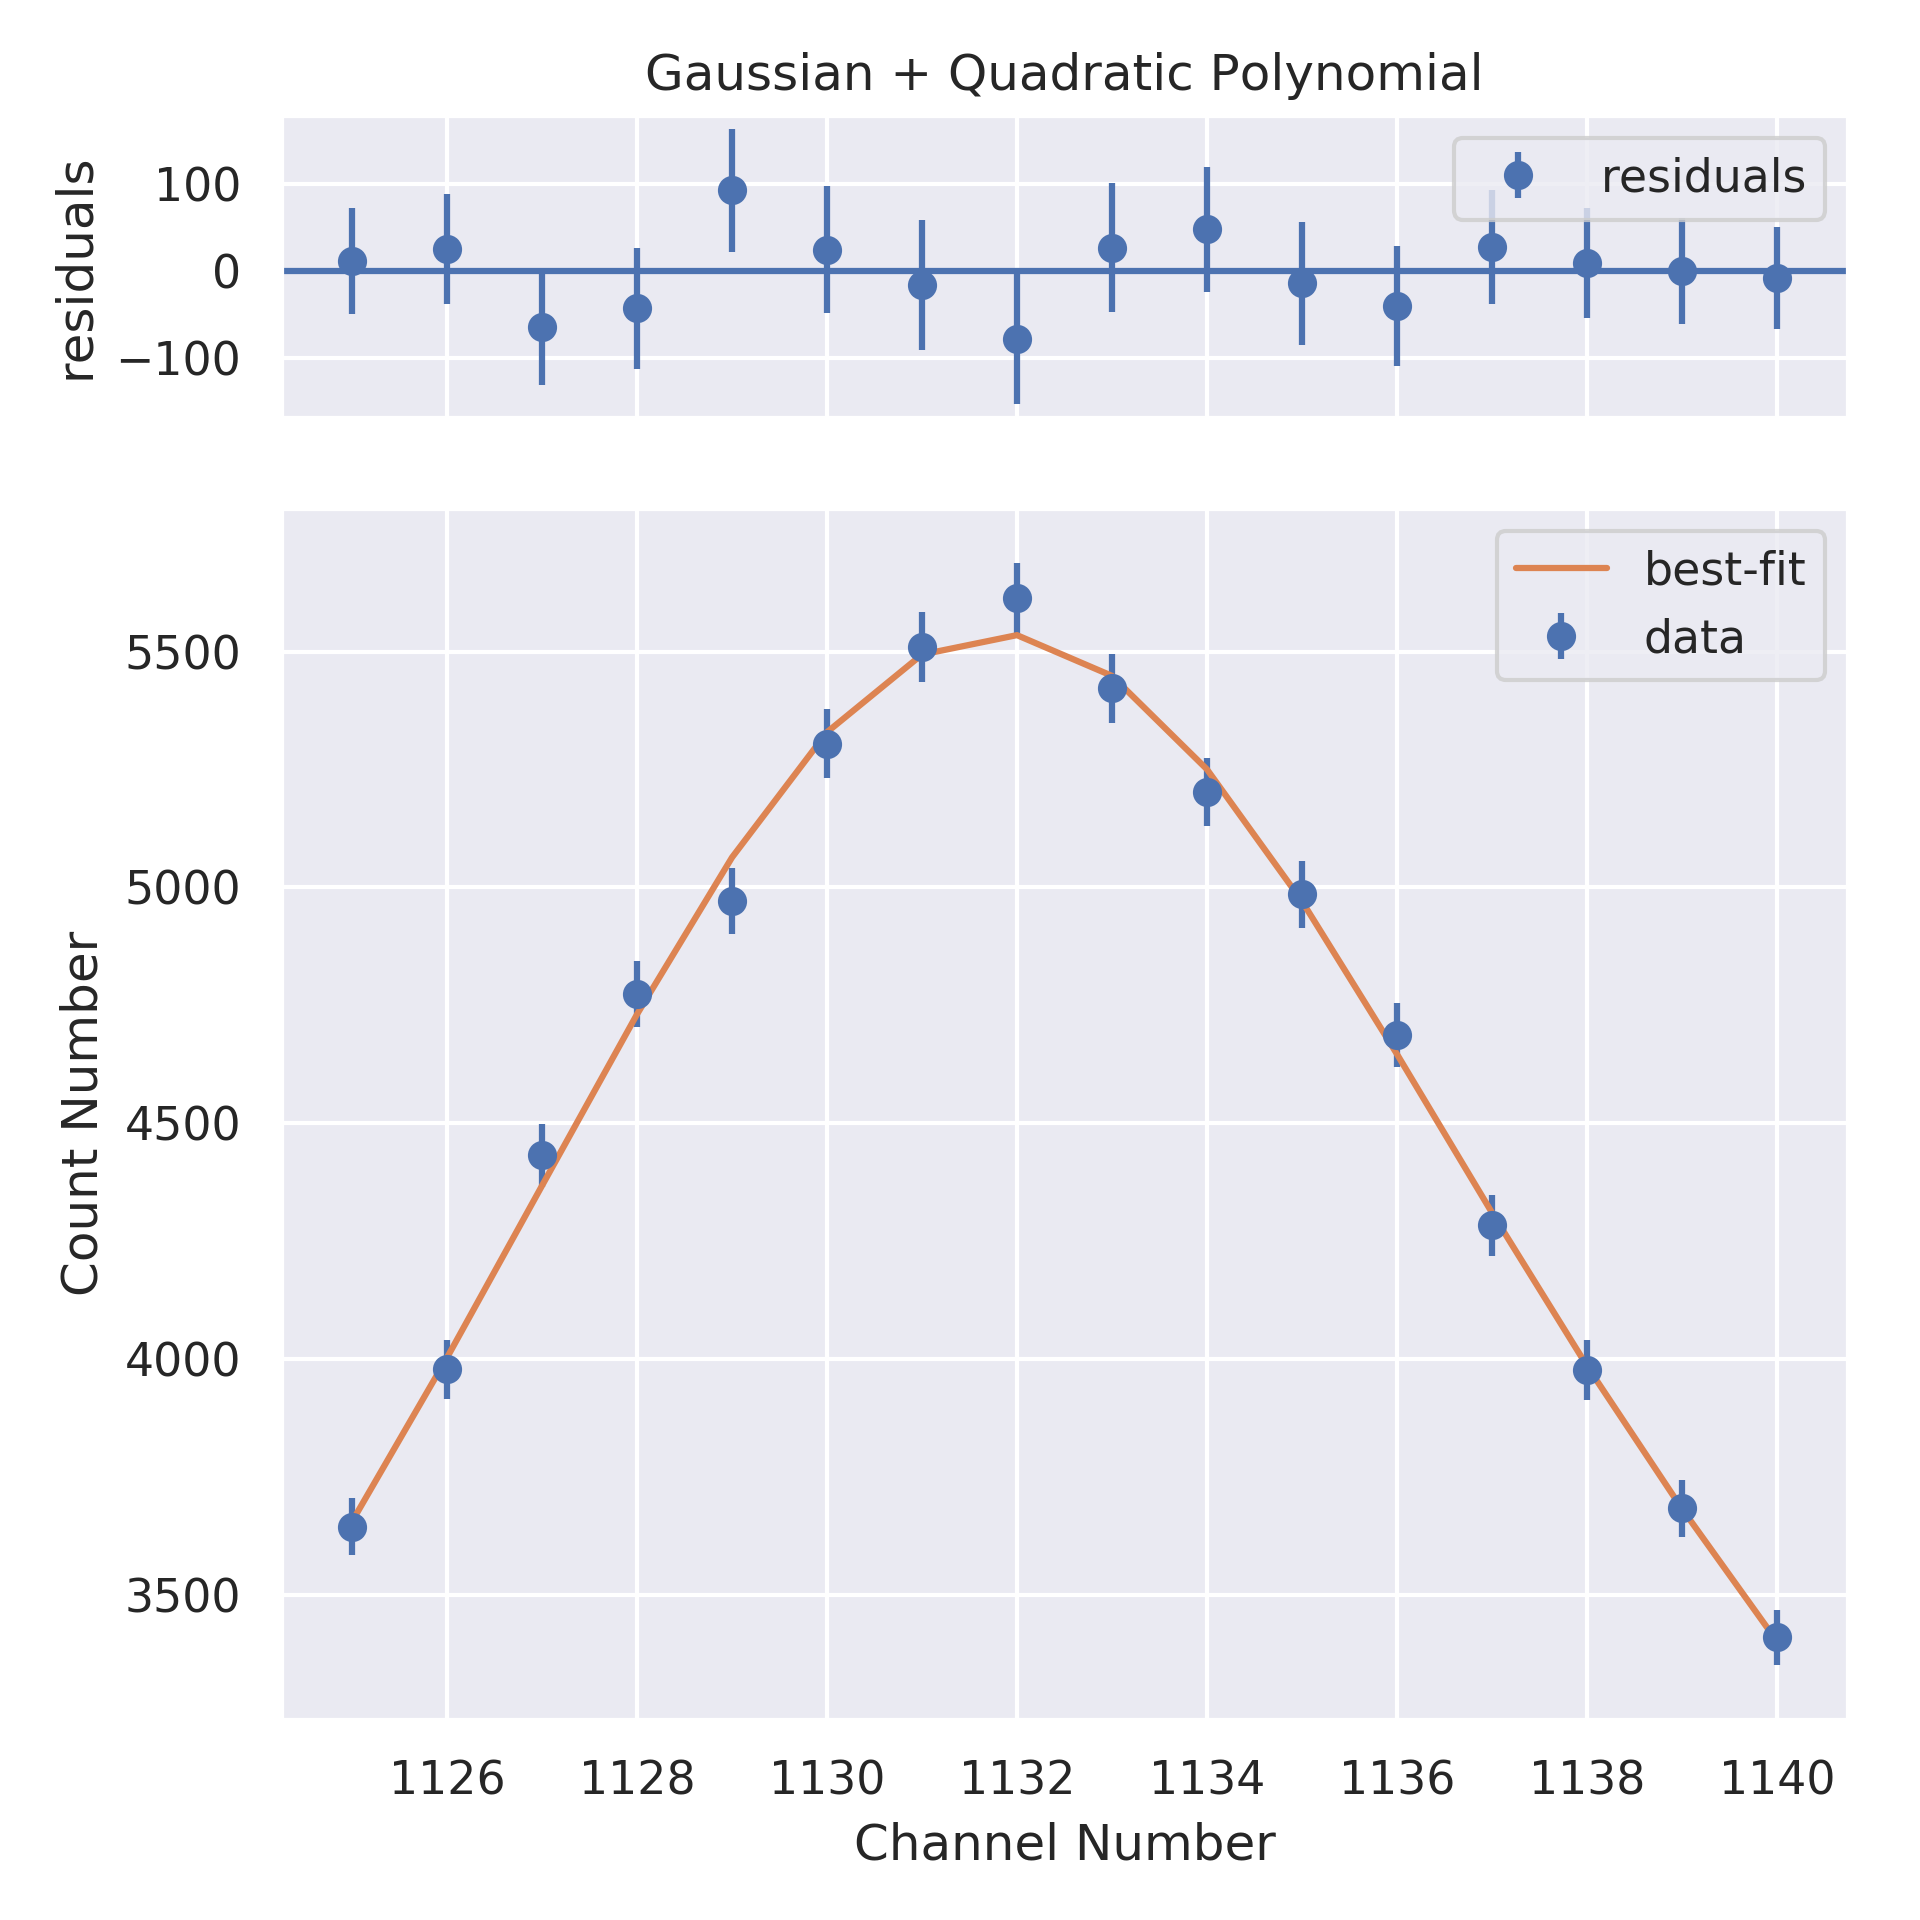
\includegraphics[width=\linewidth]{./Images/Barium133/Quad/Quad_2_Full.png}
    \caption{Full peak with fit}
    %\label{fig:sub1}
  \end{subfigure}%
  \begin{subfigure}{.5\linewidth}
    \centering
    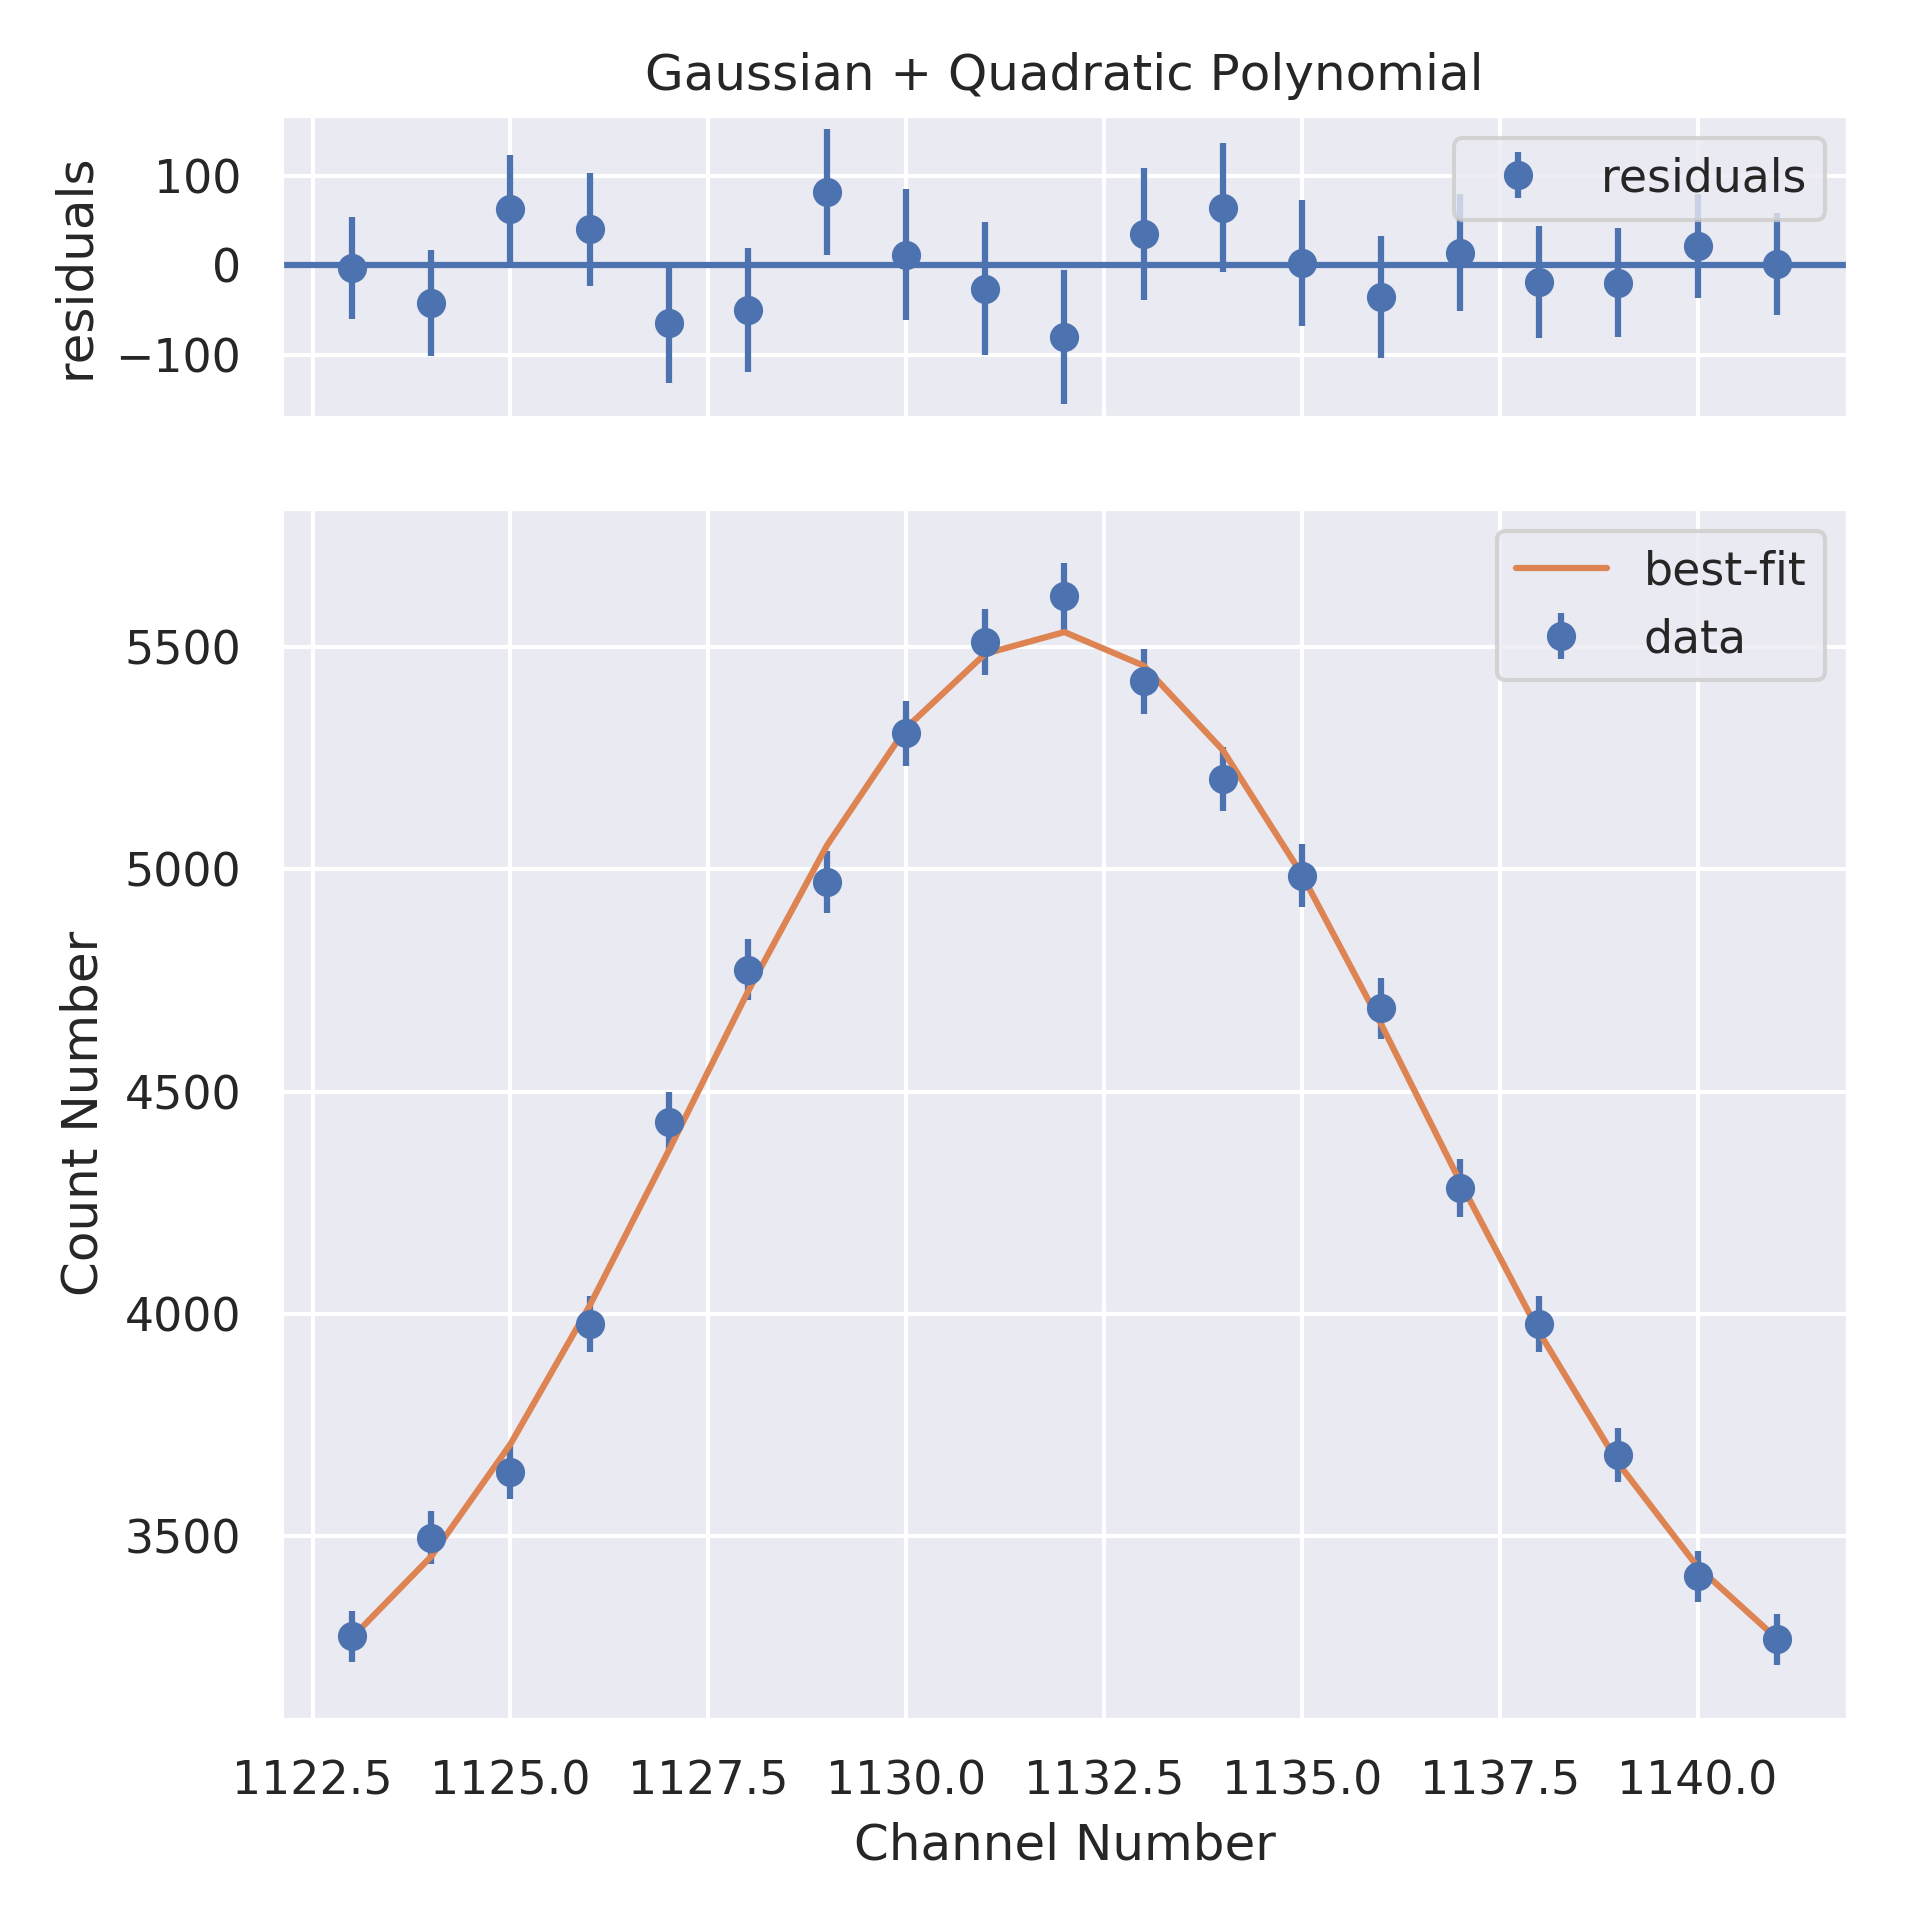
\includegraphics[width=\linewidth]{./Images/Barium133/Quad/Quad_2_Zoom.png}
    \caption{Zoomed in peak with fit}
    %\label{fig:sub2}
  \end{subfigure}
  \caption{Fit of full \& zoomed in peak of \element{Ba}{133} 161 keV peak}
  %\label{fig:test}
\end{figure}
\begin{figure}[H]
  \centering
  \begin{subfigure}{.5\linewidth}
    \centering
    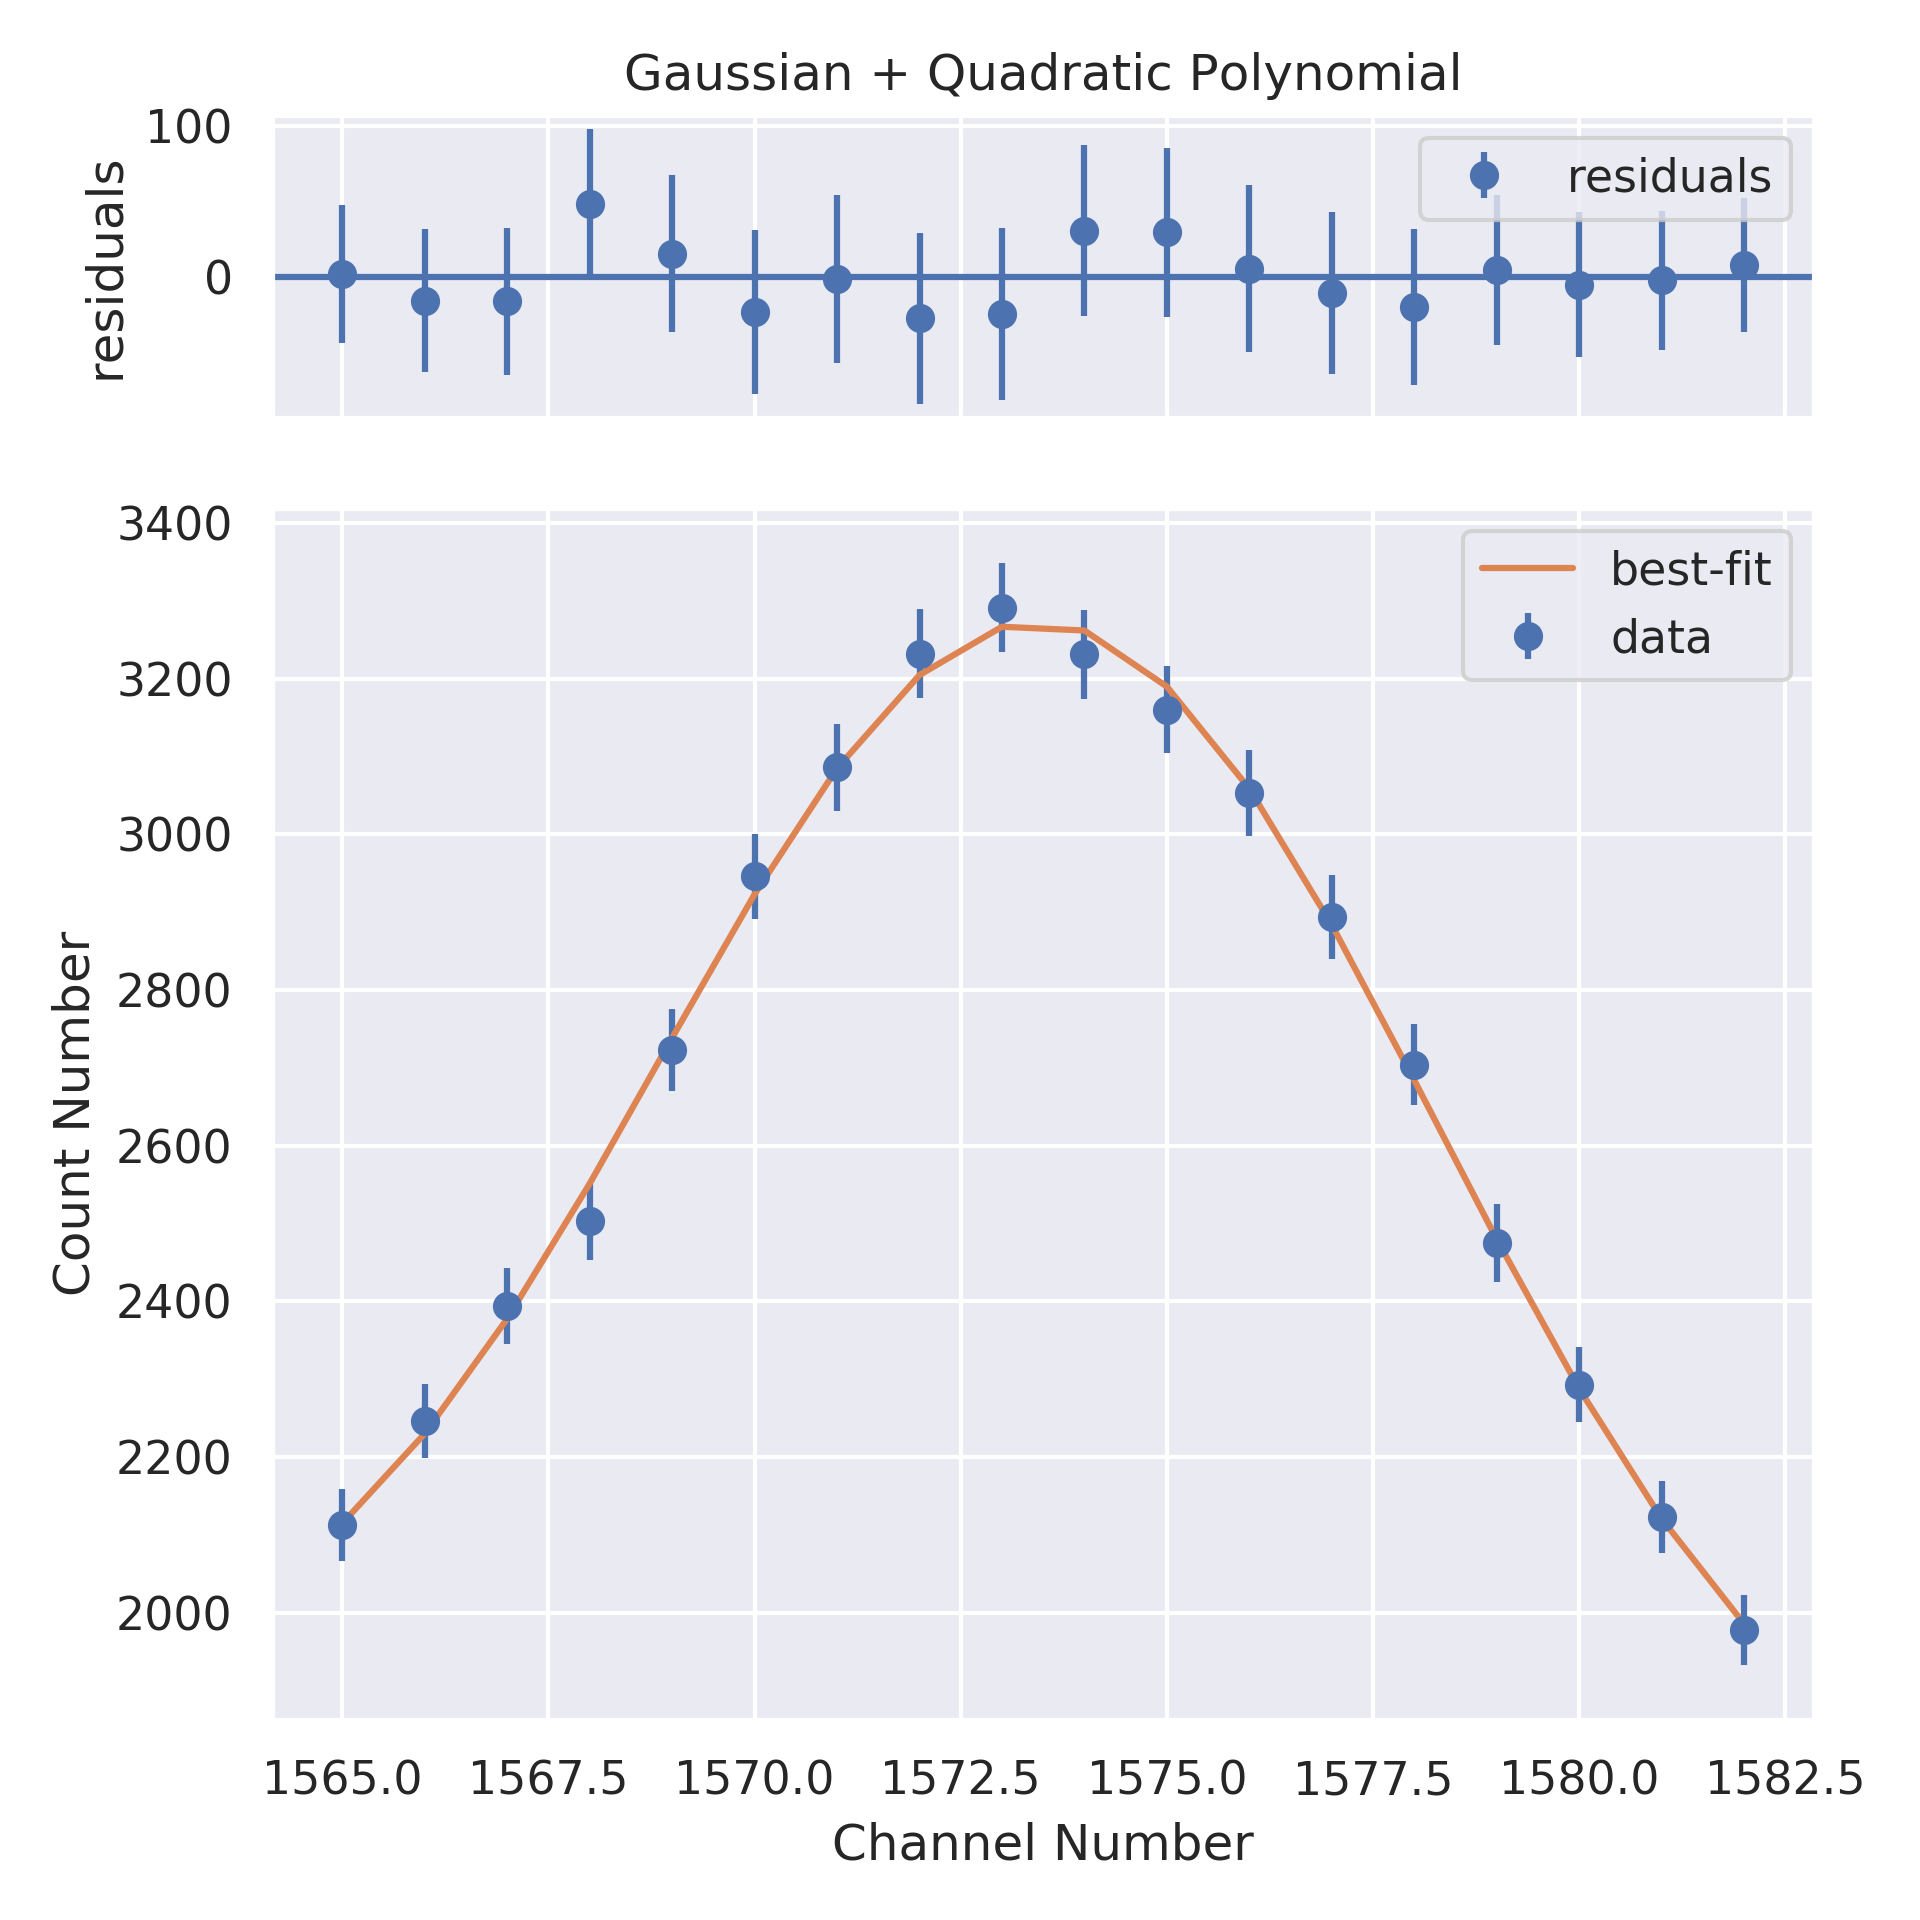
\includegraphics[width=\linewidth]{./Images/Barium133/Quad/Quad_3_Full.png}
    \caption{Full peak with fit}
    %\label{fig:sub1}
  \end{subfigure}%
  \begin{subfigure}{.5\linewidth}
    \centering
    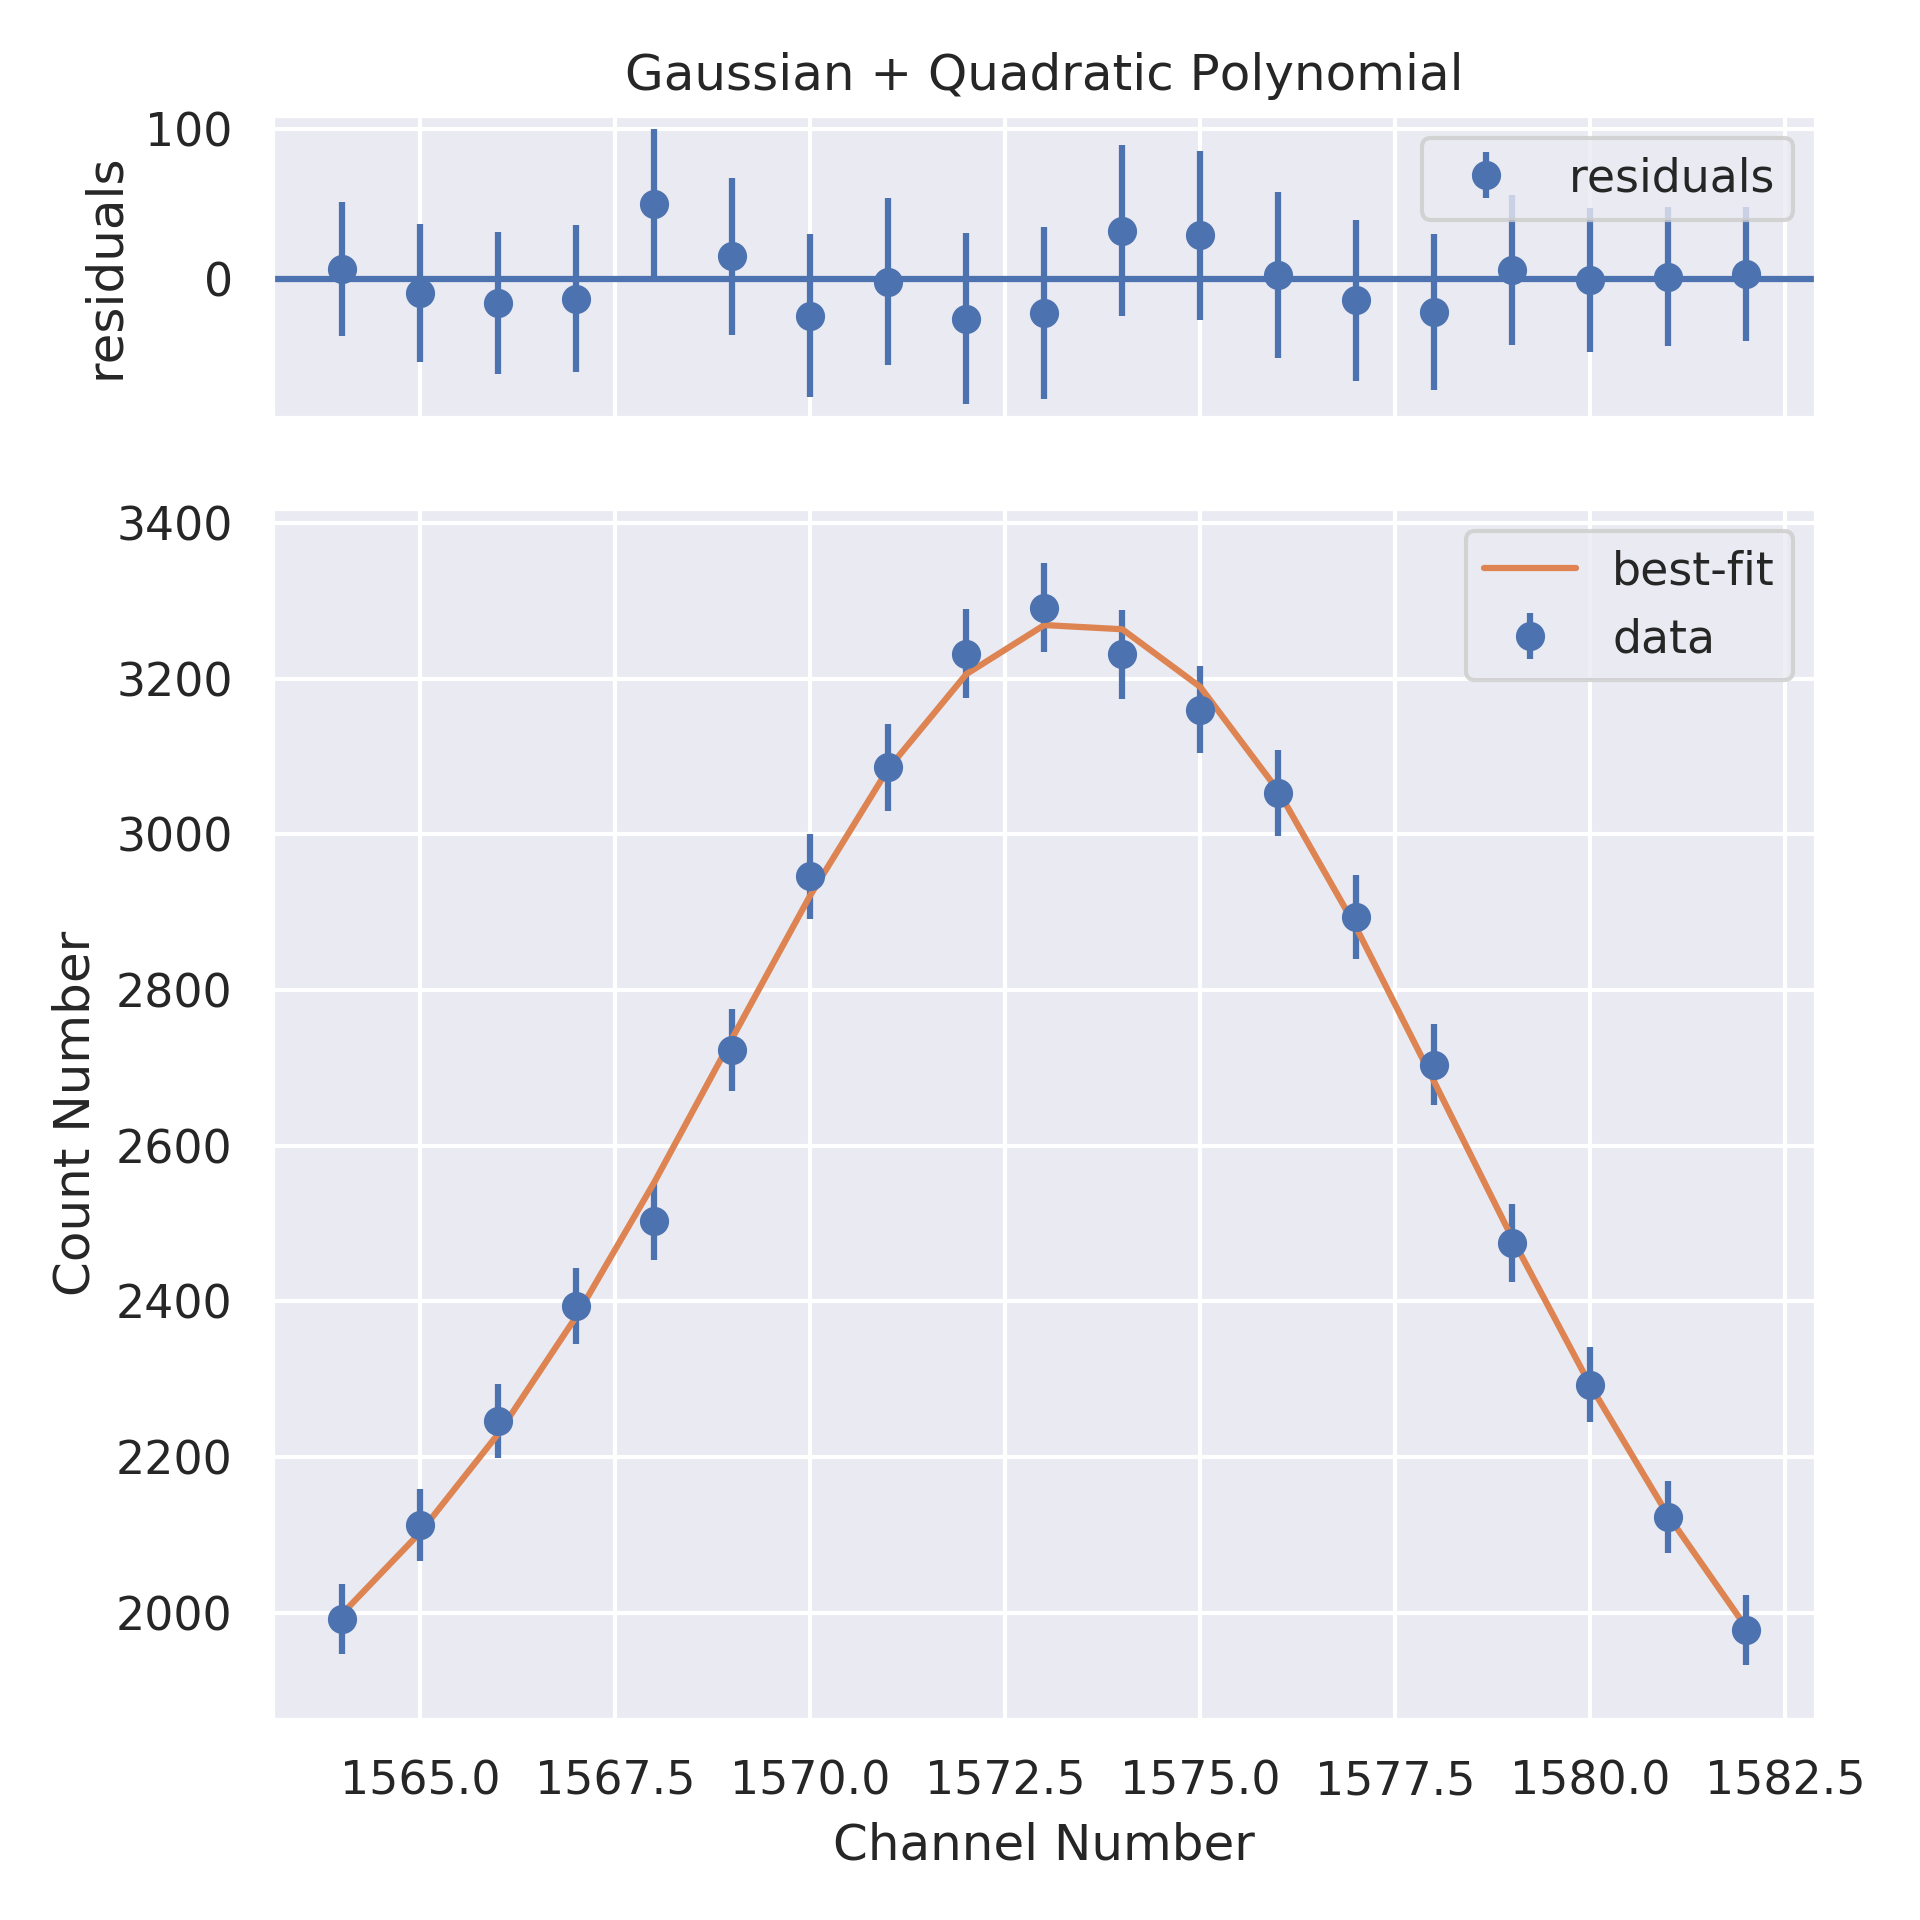
\includegraphics[width=\linewidth]{./Images/Barium133/Quad/Quad_3_Zoom.png}
    \caption{Zoomed in peak with fit}
    %\label{fig:sub2}
  \end{subfigure}
  \caption{Fit of full \& zoomed in peak of \element{Ba}{133} 223 keV peak}
  %\label{fig:test}
\end{figure}
\begin{figure}[H]
  \centering
  \begin{subfigure}{.5\linewidth}
    \centering
    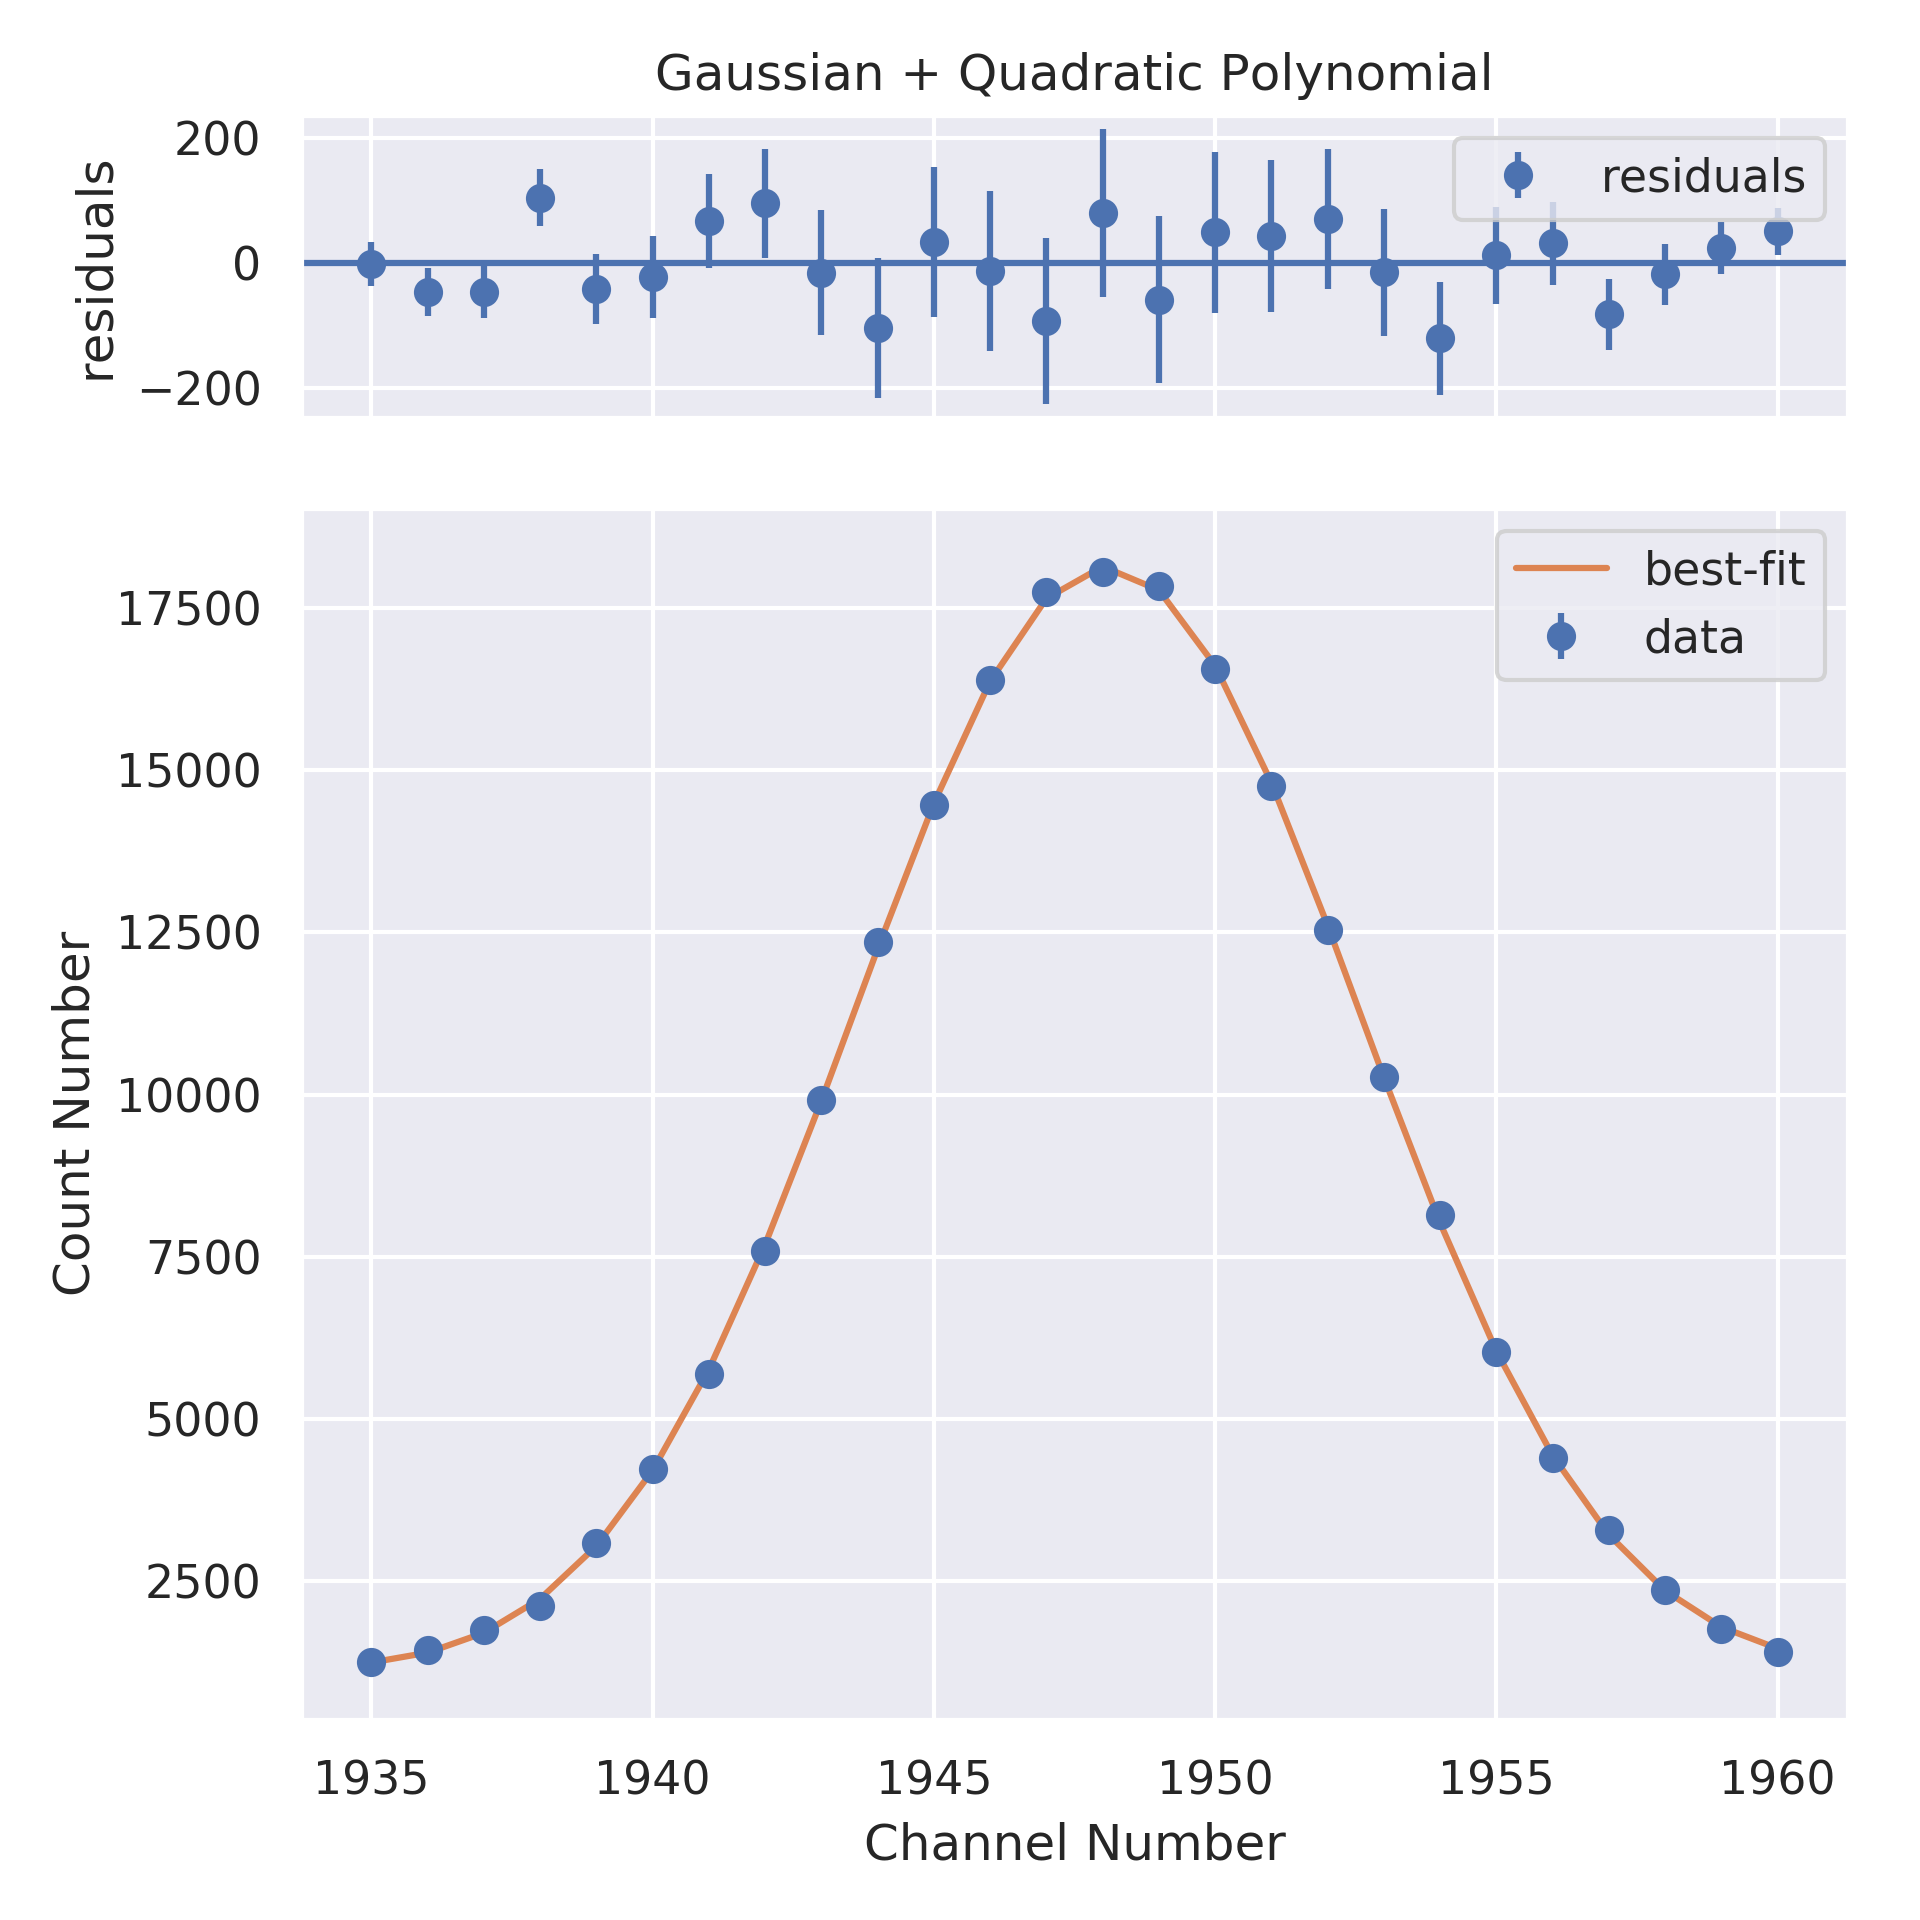
\includegraphics[width=\linewidth]{./Images/Barium133/Quad/Quad_4_Full.png}
    \caption{Full peak with fit}
    %\label{fig:sub1}
  \end{subfigure}%
  \begin{subfigure}{.5\linewidth}
    \centering
    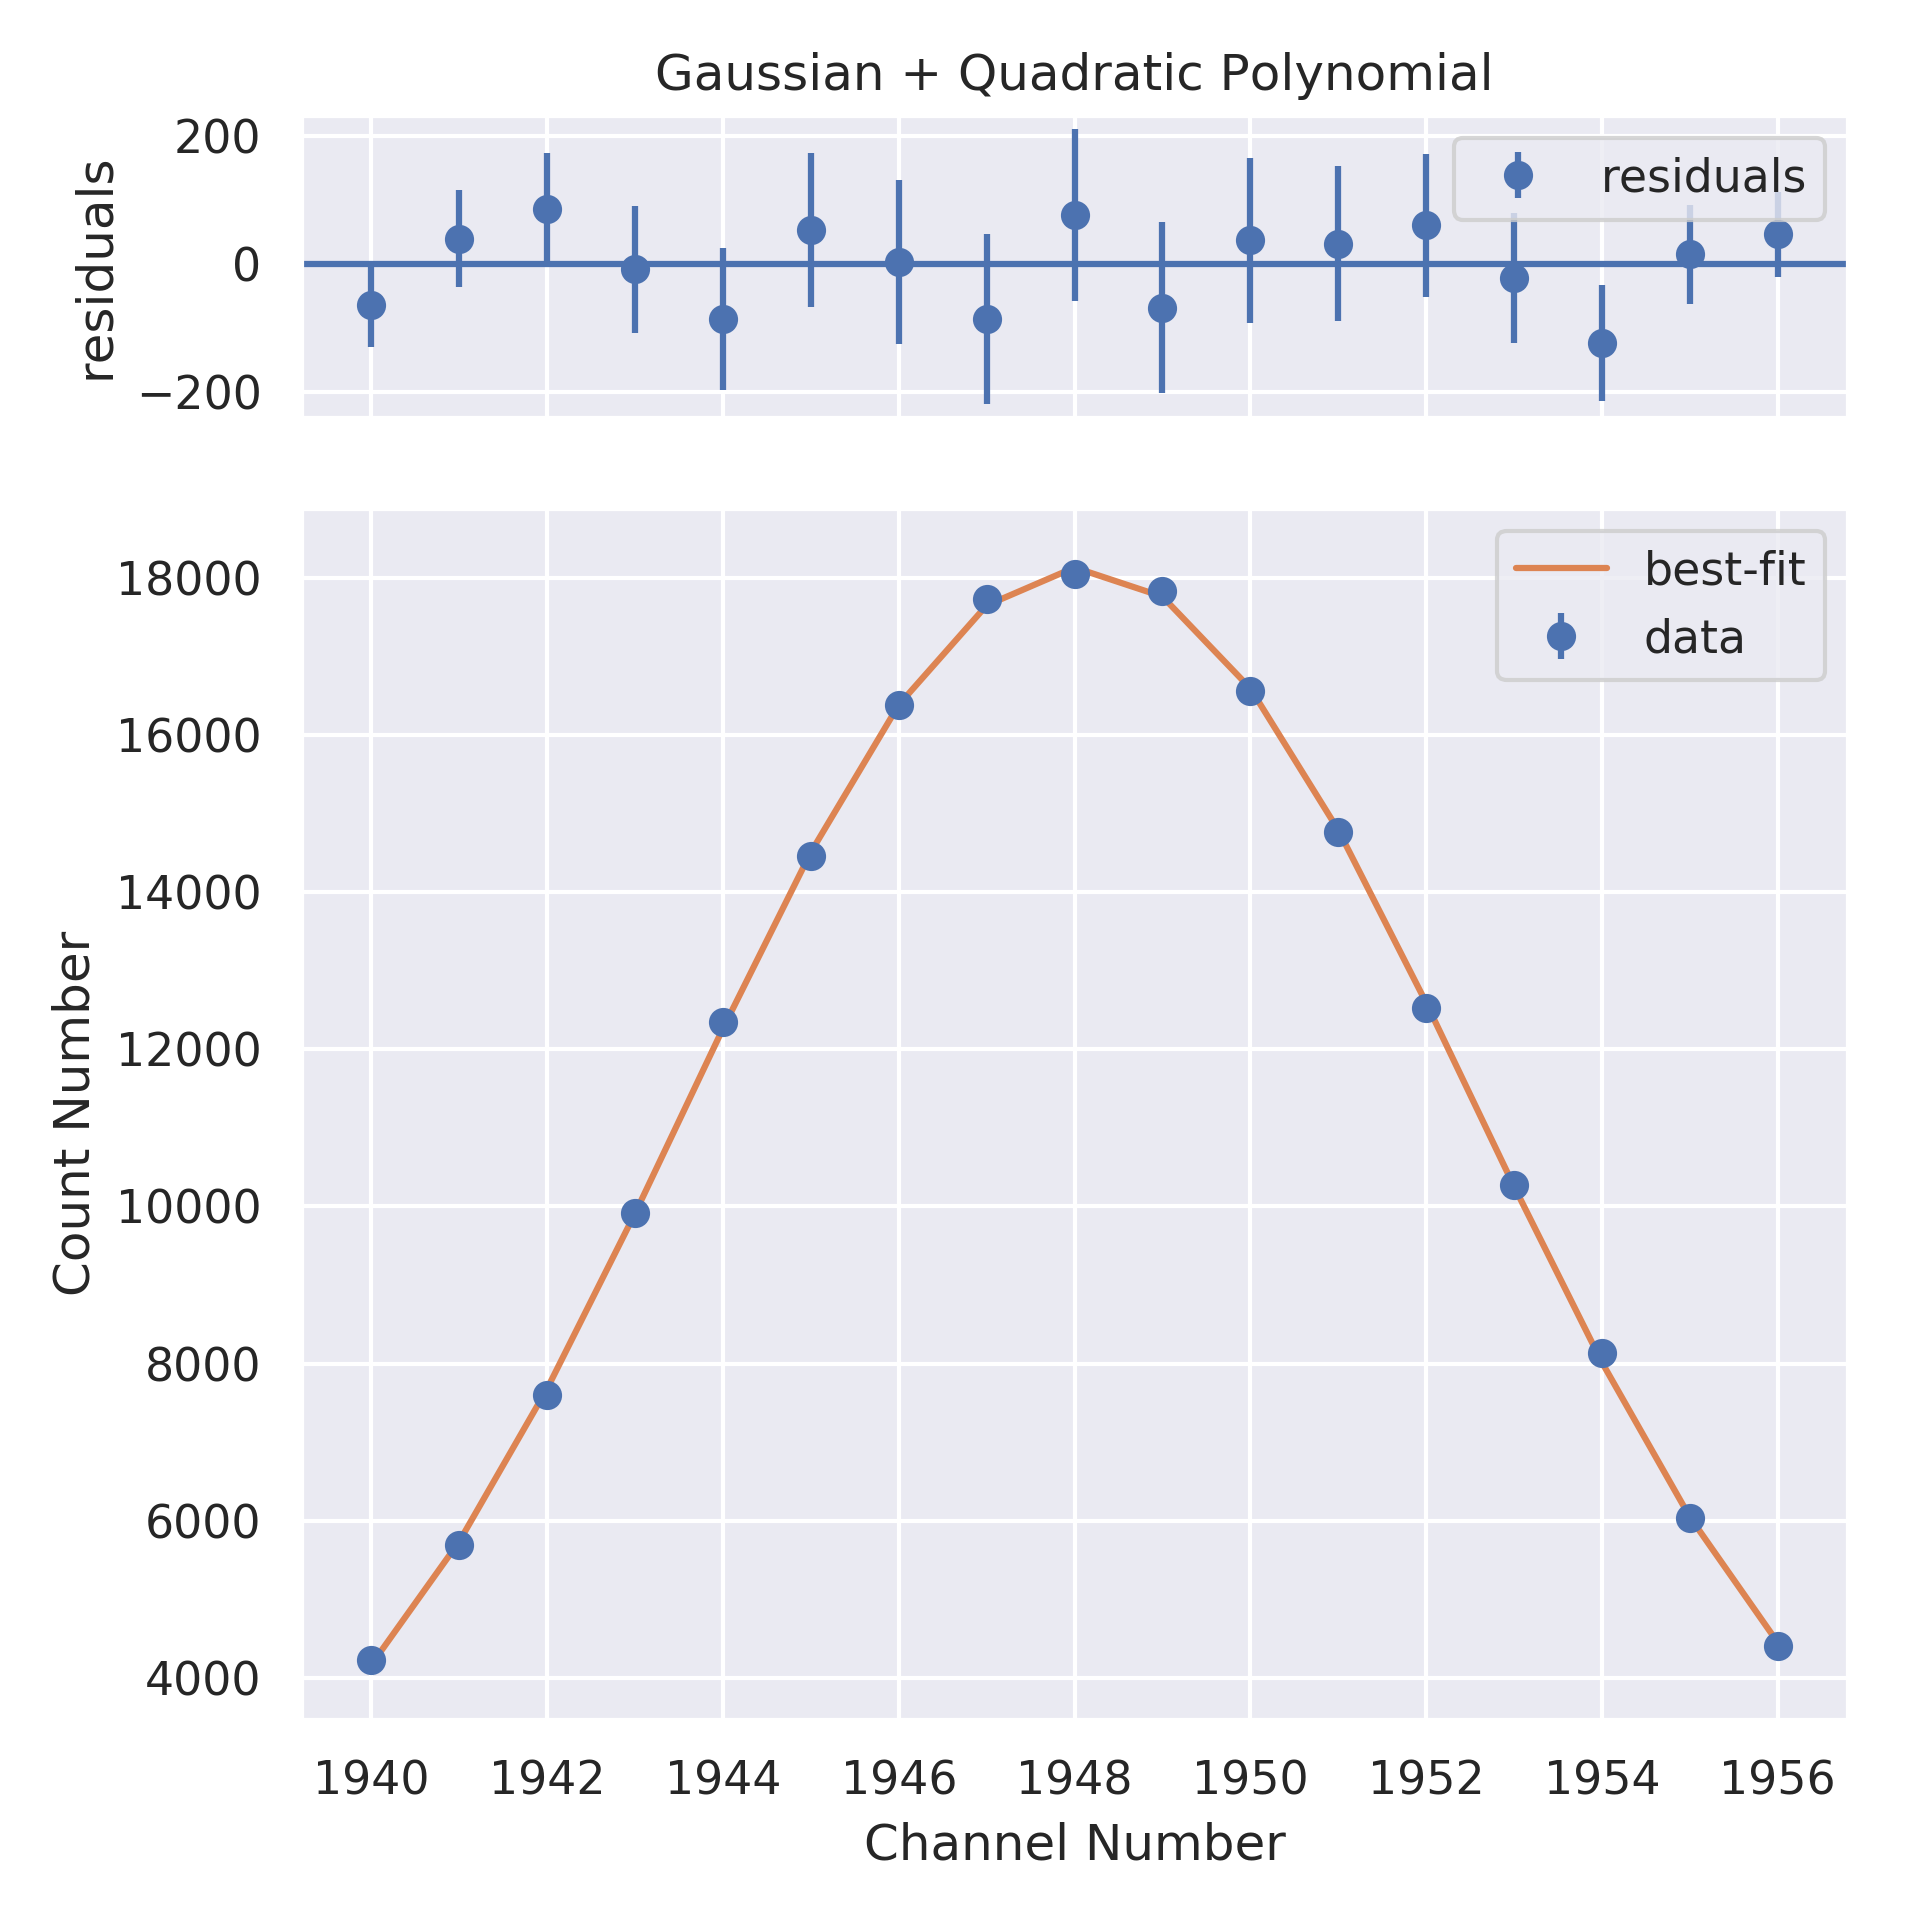
\includegraphics[width=\linewidth]{./Images/Barium133/Quad/Quad_4_Zoom.png}
    \caption{Zoomed in peak with fit}
    %\label{fig:sub2}
  \end{subfigure}
  \caption{Fit of full \& zoomed in peak of \element{Ba}{133} 276 keV peak}
  %\label{fig:test}
\end{figure}
\begin{figure}[H]
  \centering
  \begin{subfigure}{.5\linewidth}
    \centering
    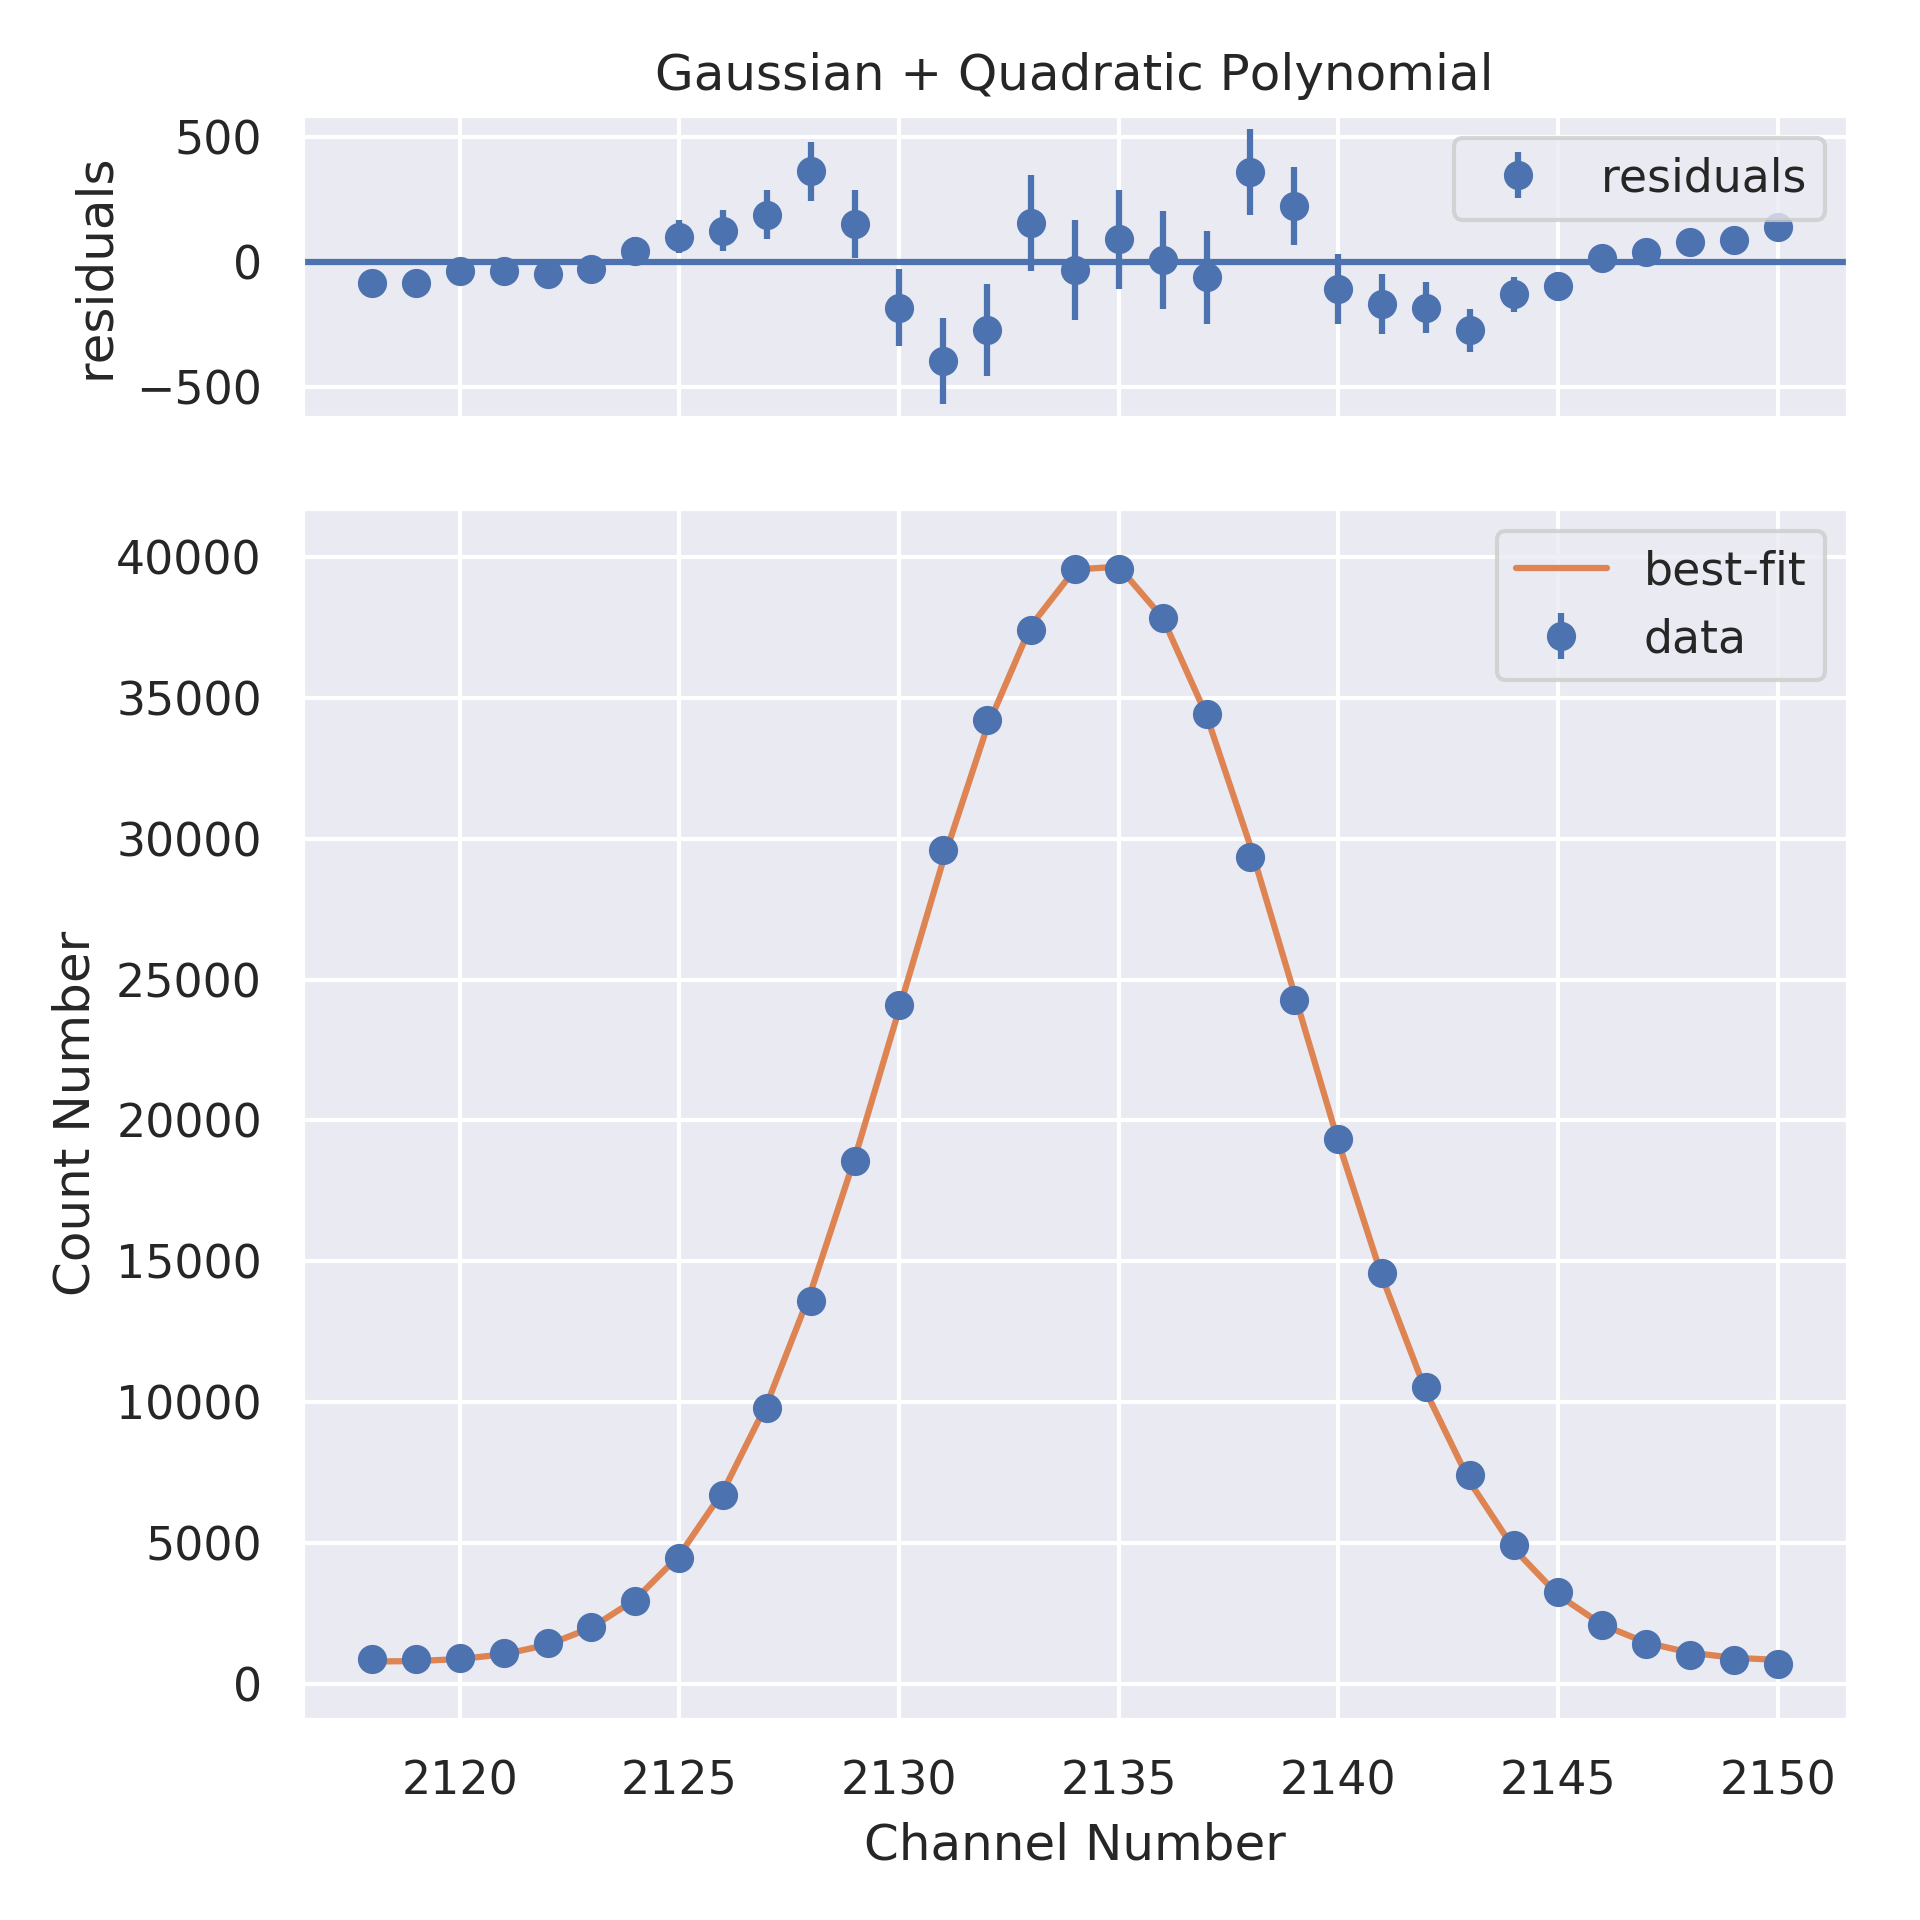
\includegraphics[width=\linewidth]{./Images/Barium133/Quad/Quad_5_Full.png}
    \caption{Full peak with fit}
    %\label{fig:sub1}
  \end{subfigure}%
  \begin{subfigure}{.5\linewidth}
    \centering
    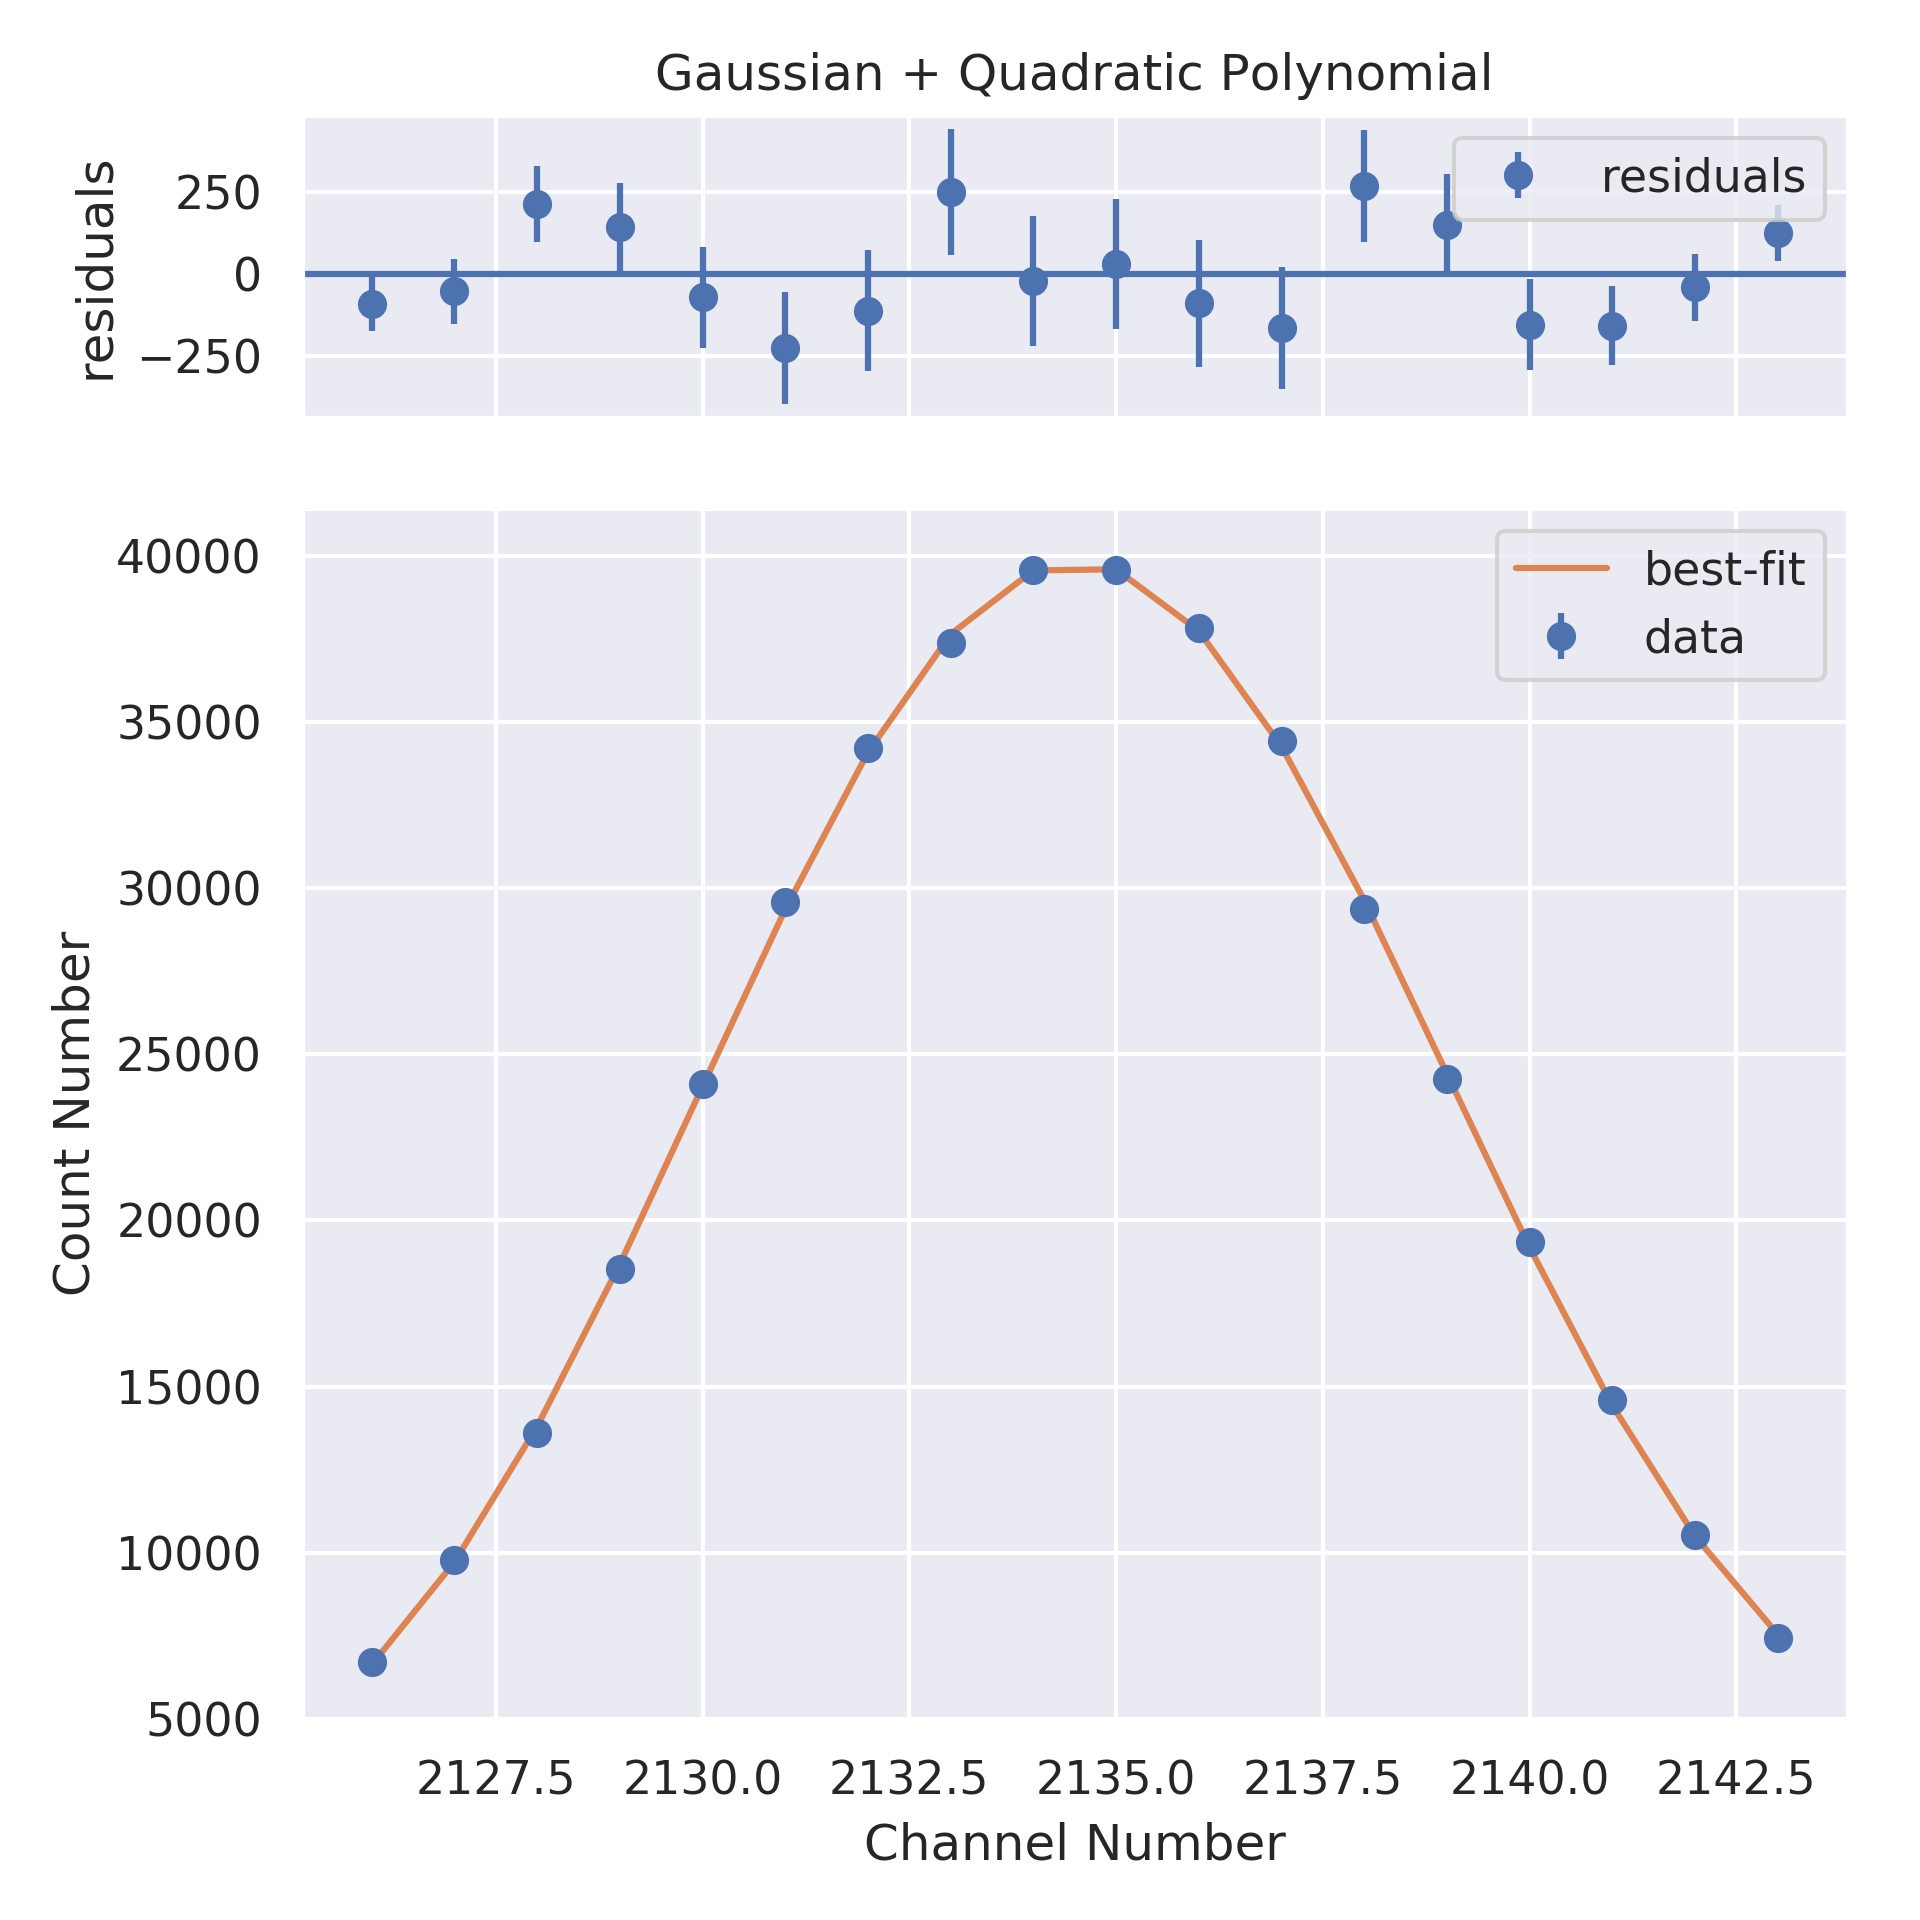
\includegraphics[width=\linewidth]{./Images/Barium133/Quad/Quad_5_Zoom.png}
    \caption{Zoomed in peak with fit}
    %\label{fig:sub2}
  \end{subfigure}
  \caption{Fit of full \& zoomed in peak of \element{Ba}{133} 303 keV peak}
  %\label{fig:test}
\end{figure}
\begin{figure}[H]
  \centering
  \begin{subfigure}{.5\linewidth}
    \centering
    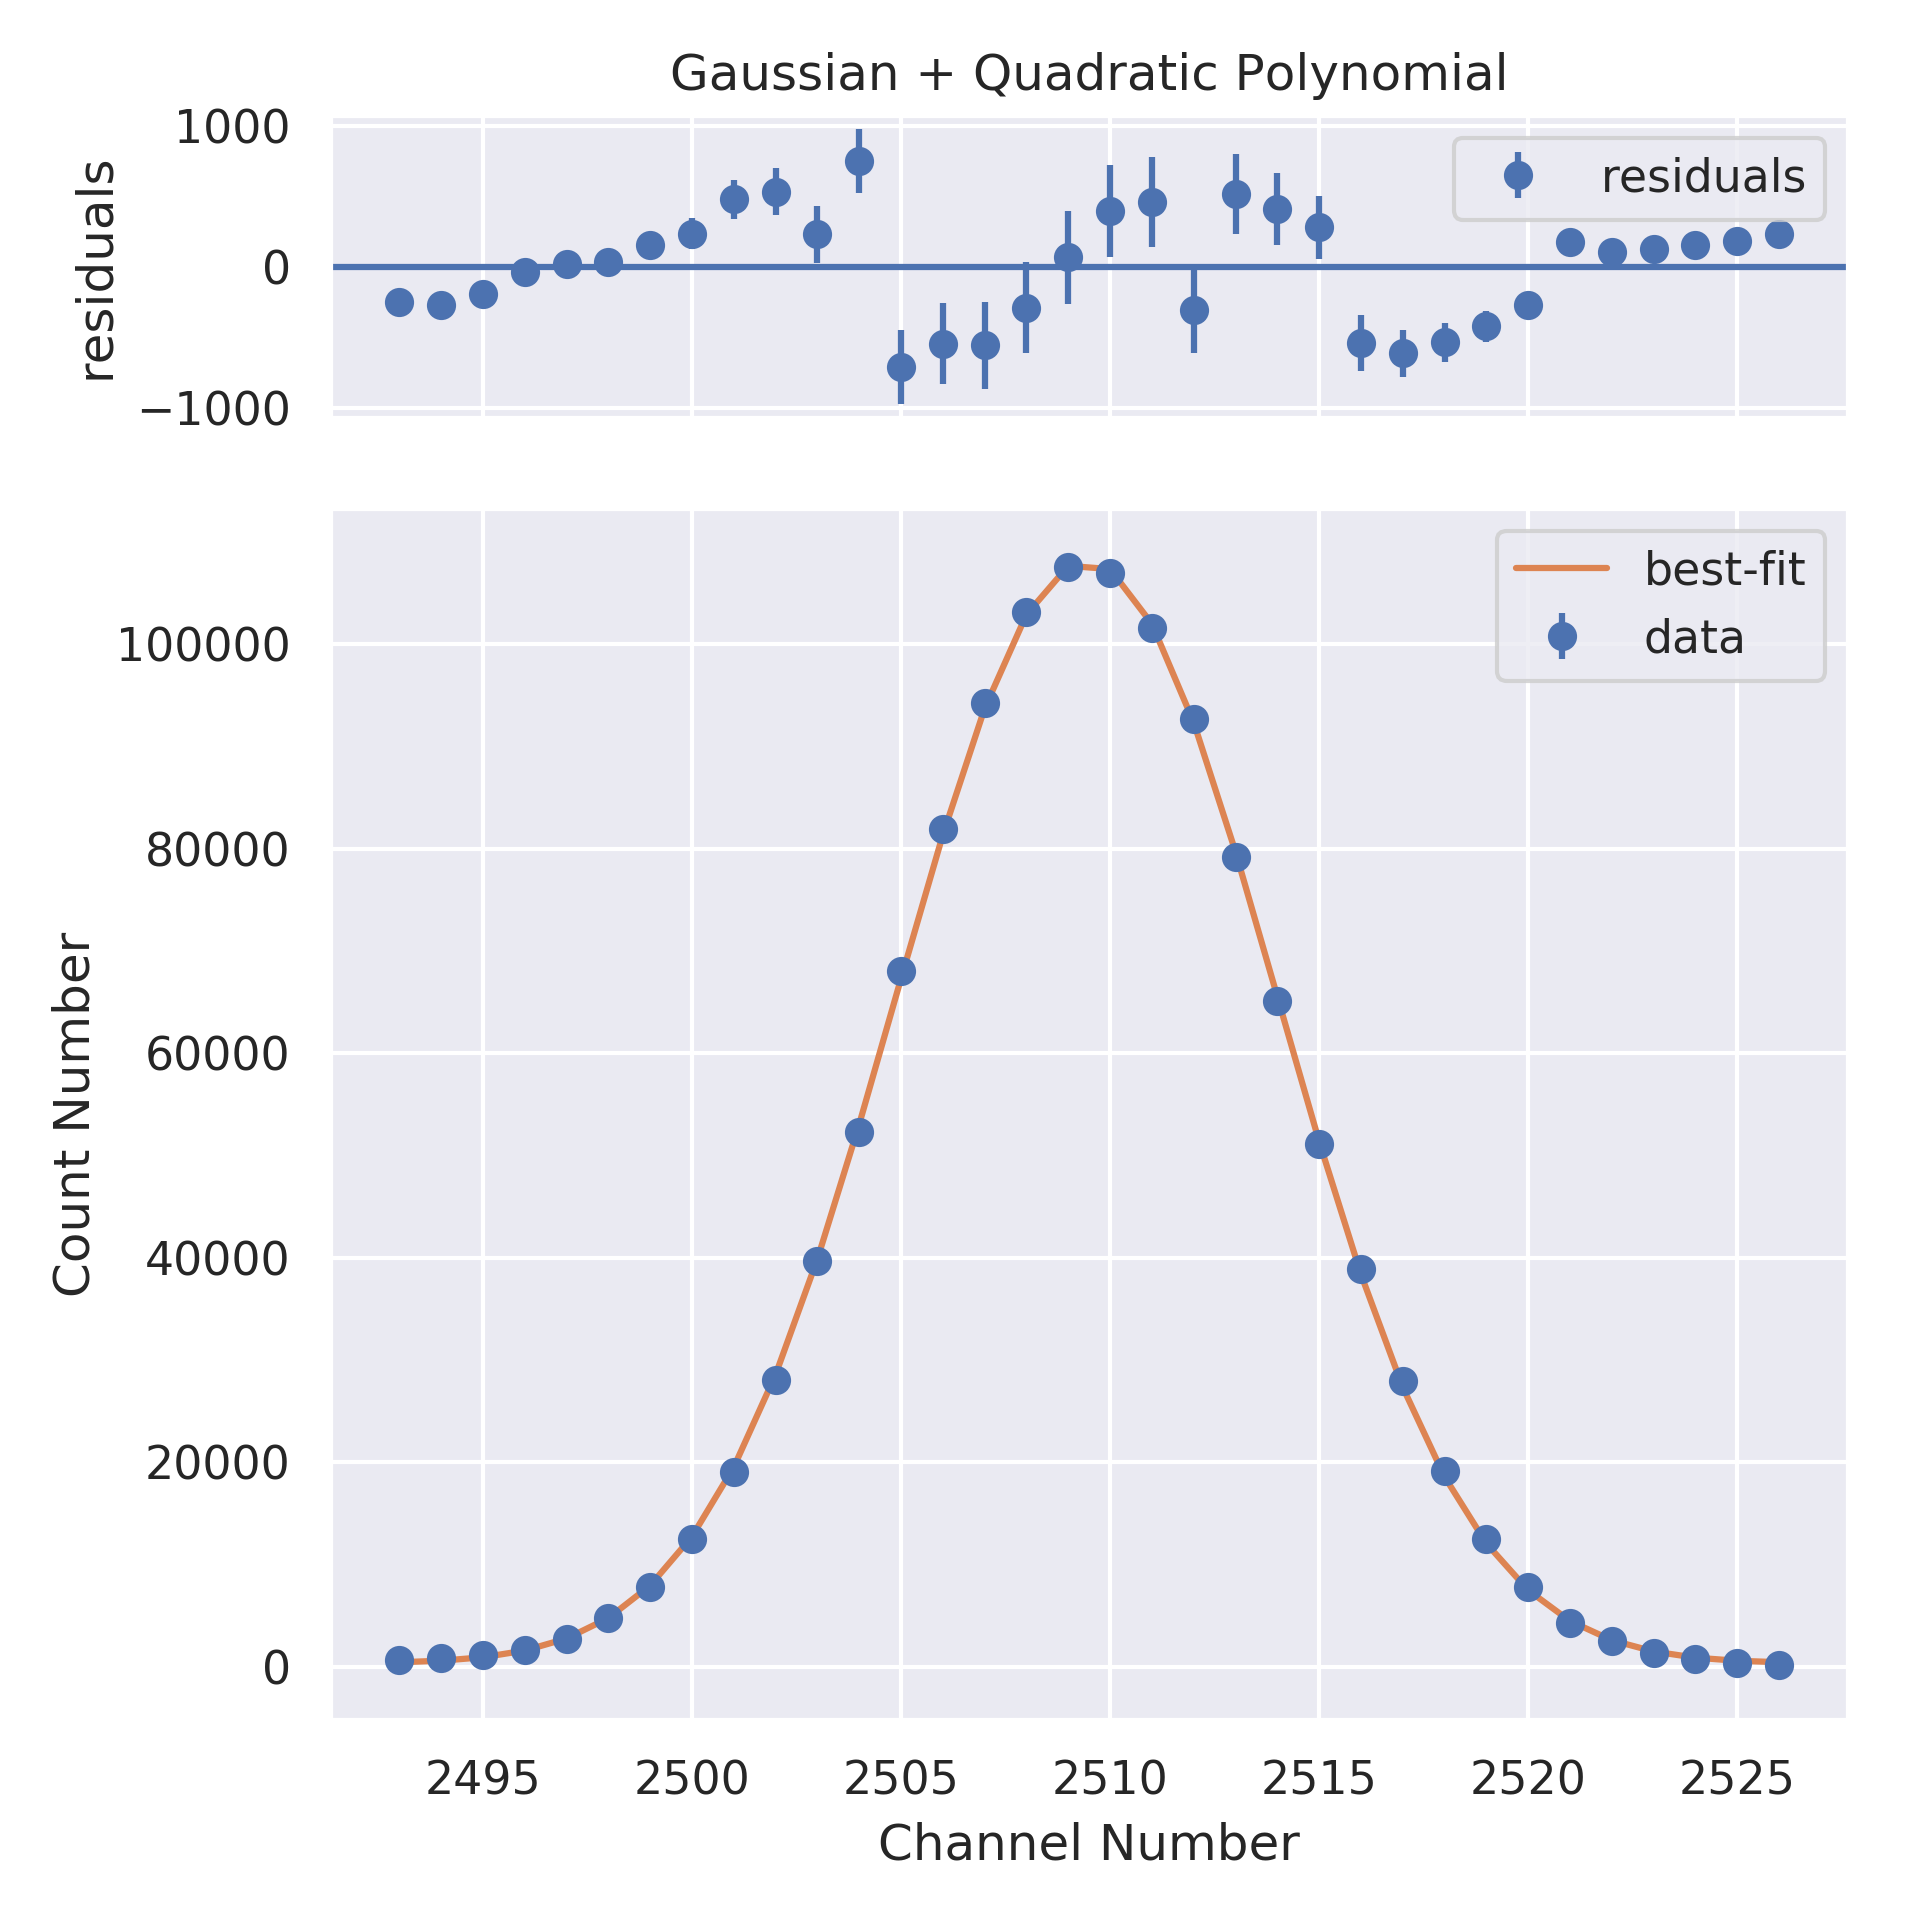
\includegraphics[width=\linewidth]{./Images/Barium133/Quad/Quad_6_Full.png}
    \caption{Full peak with fit}
    %\label{fig:sub1}
  \end{subfigure}%
  \begin{subfigure}{.5\linewidth}
    \centering
    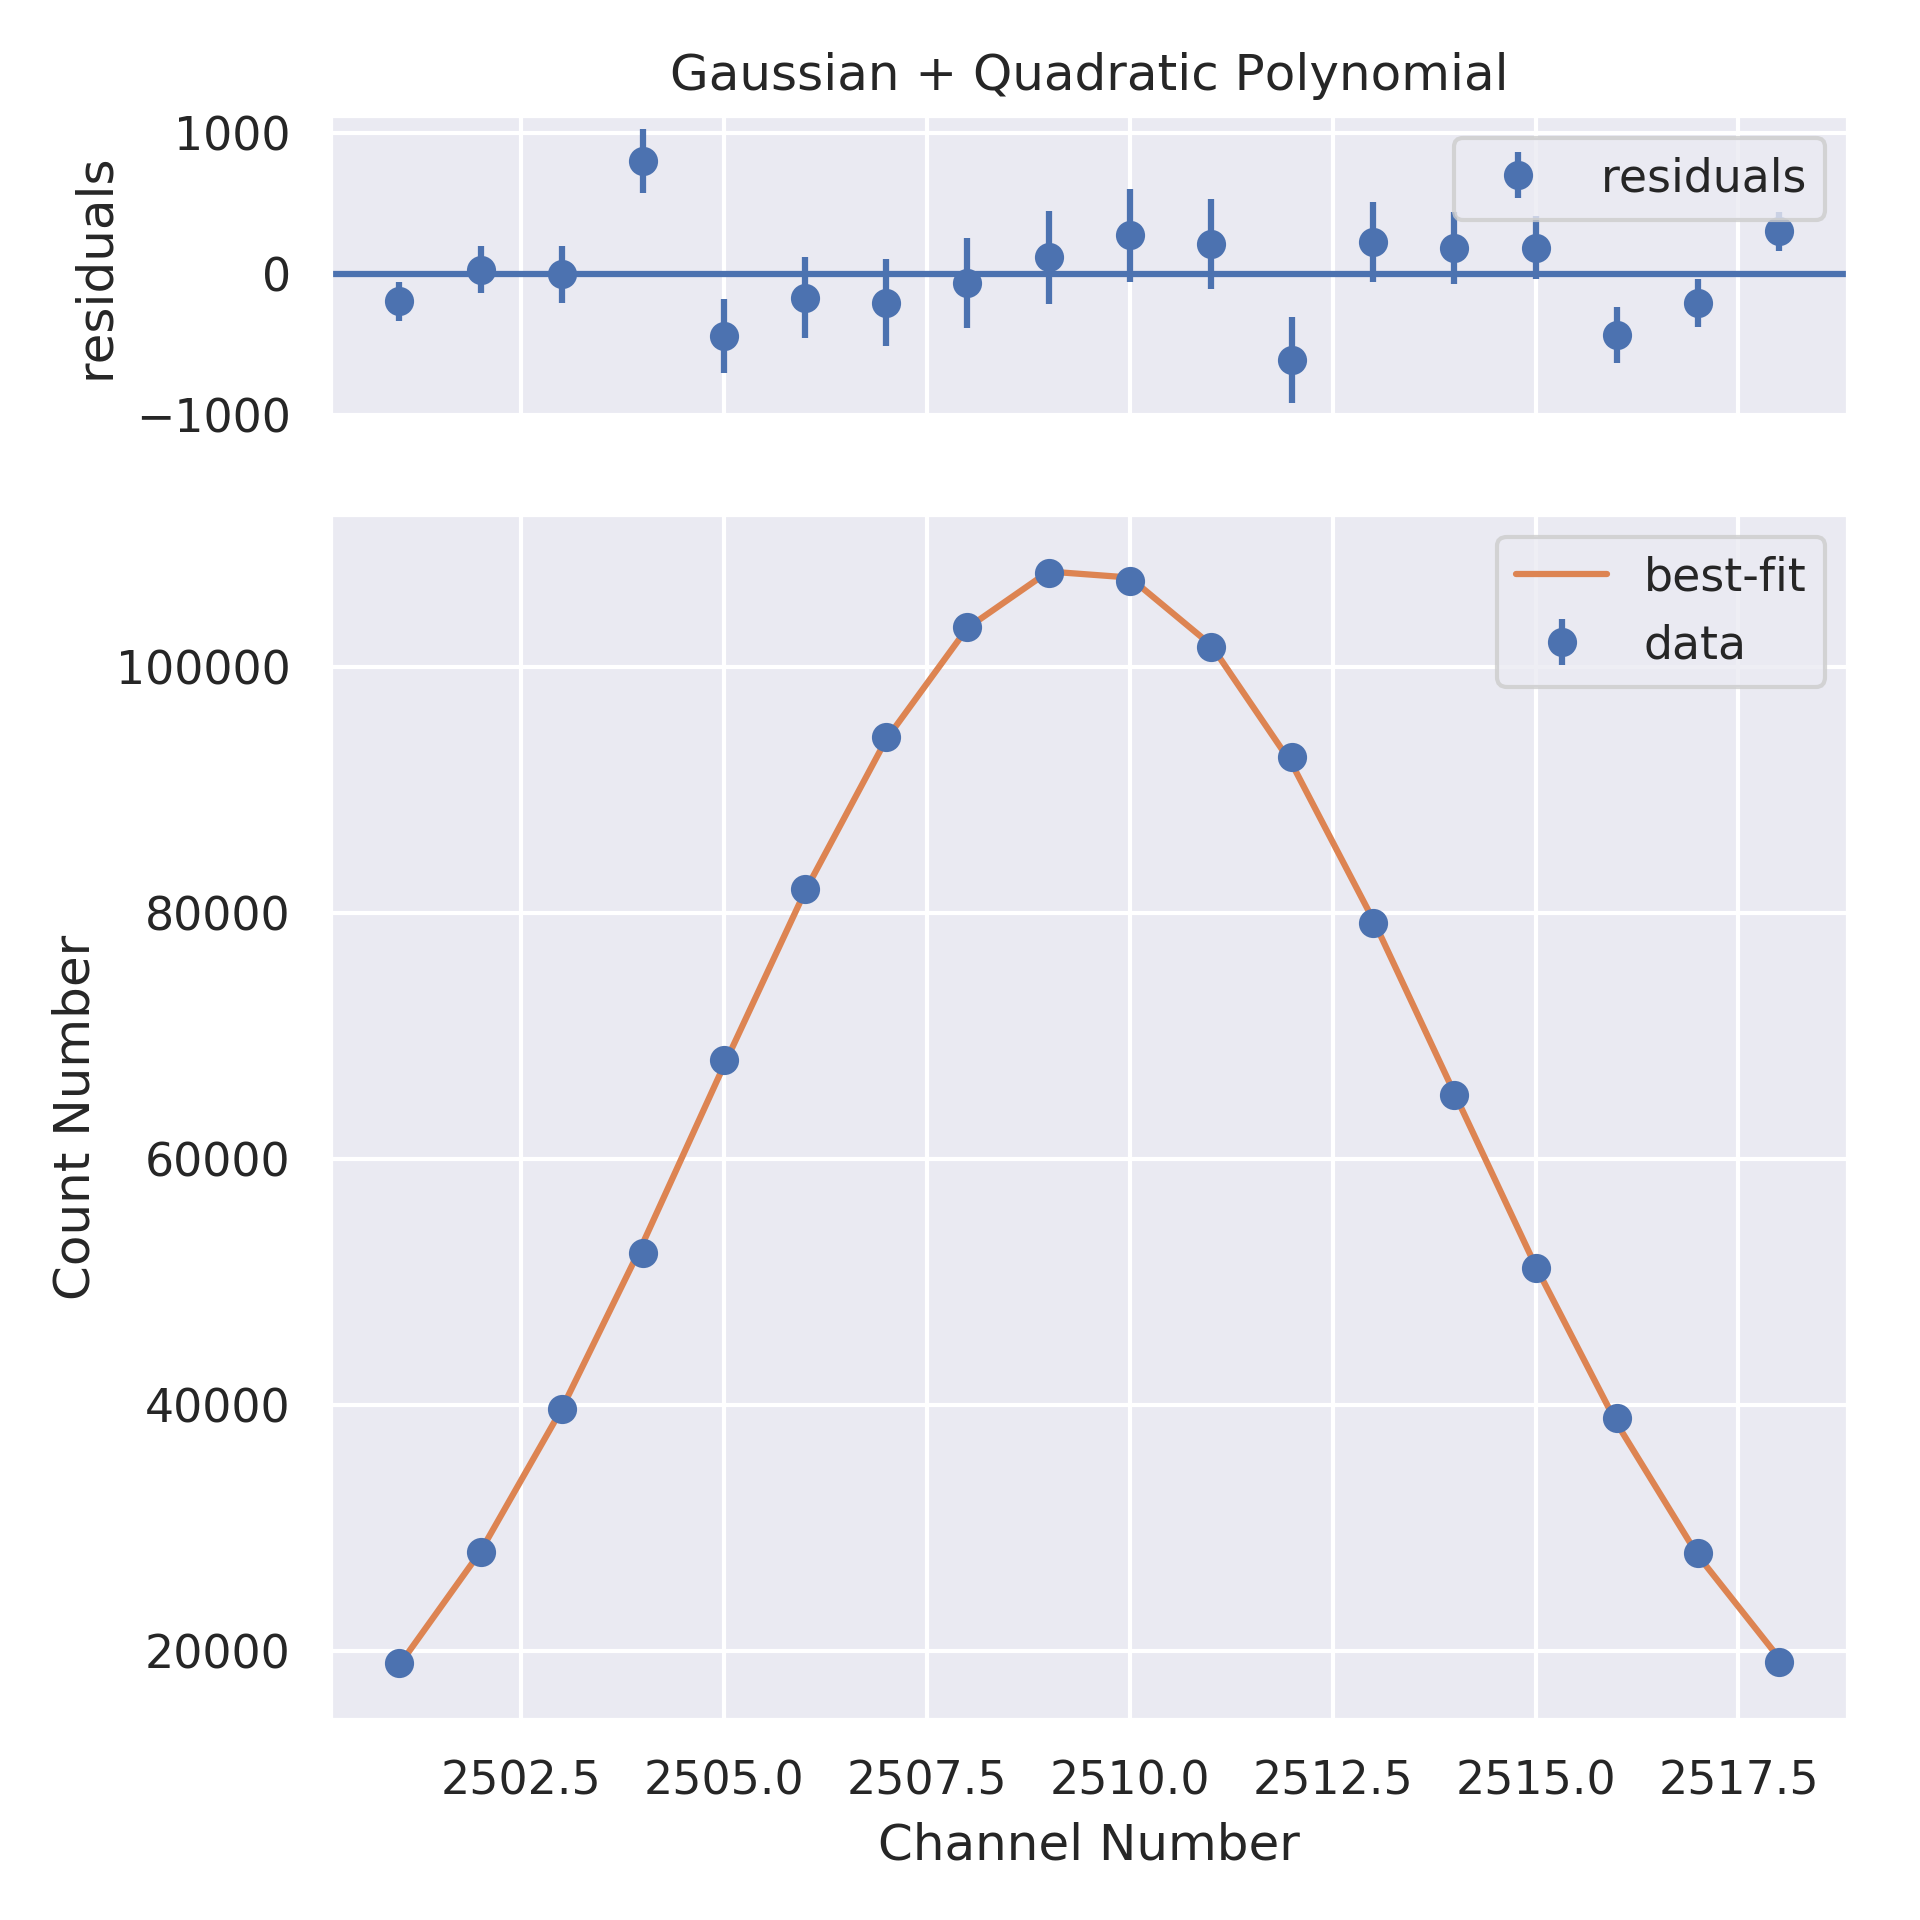
\includegraphics[width=\linewidth]{./Images/Barium133/Quad/Quad_6_Zoom.png}
    \caption{Zoomed in peak with fit}
    %\label{fig:sub2}
  \end{subfigure}
  \caption{Fit of full \& zoomed in peak of \element{Ba}{133} 356 keV peak}
  %\label{fig:test}
\end{figure}
\begin{figure}[H]
  \centering
  \begin{subfigure}{.5\linewidth}
    \centering
    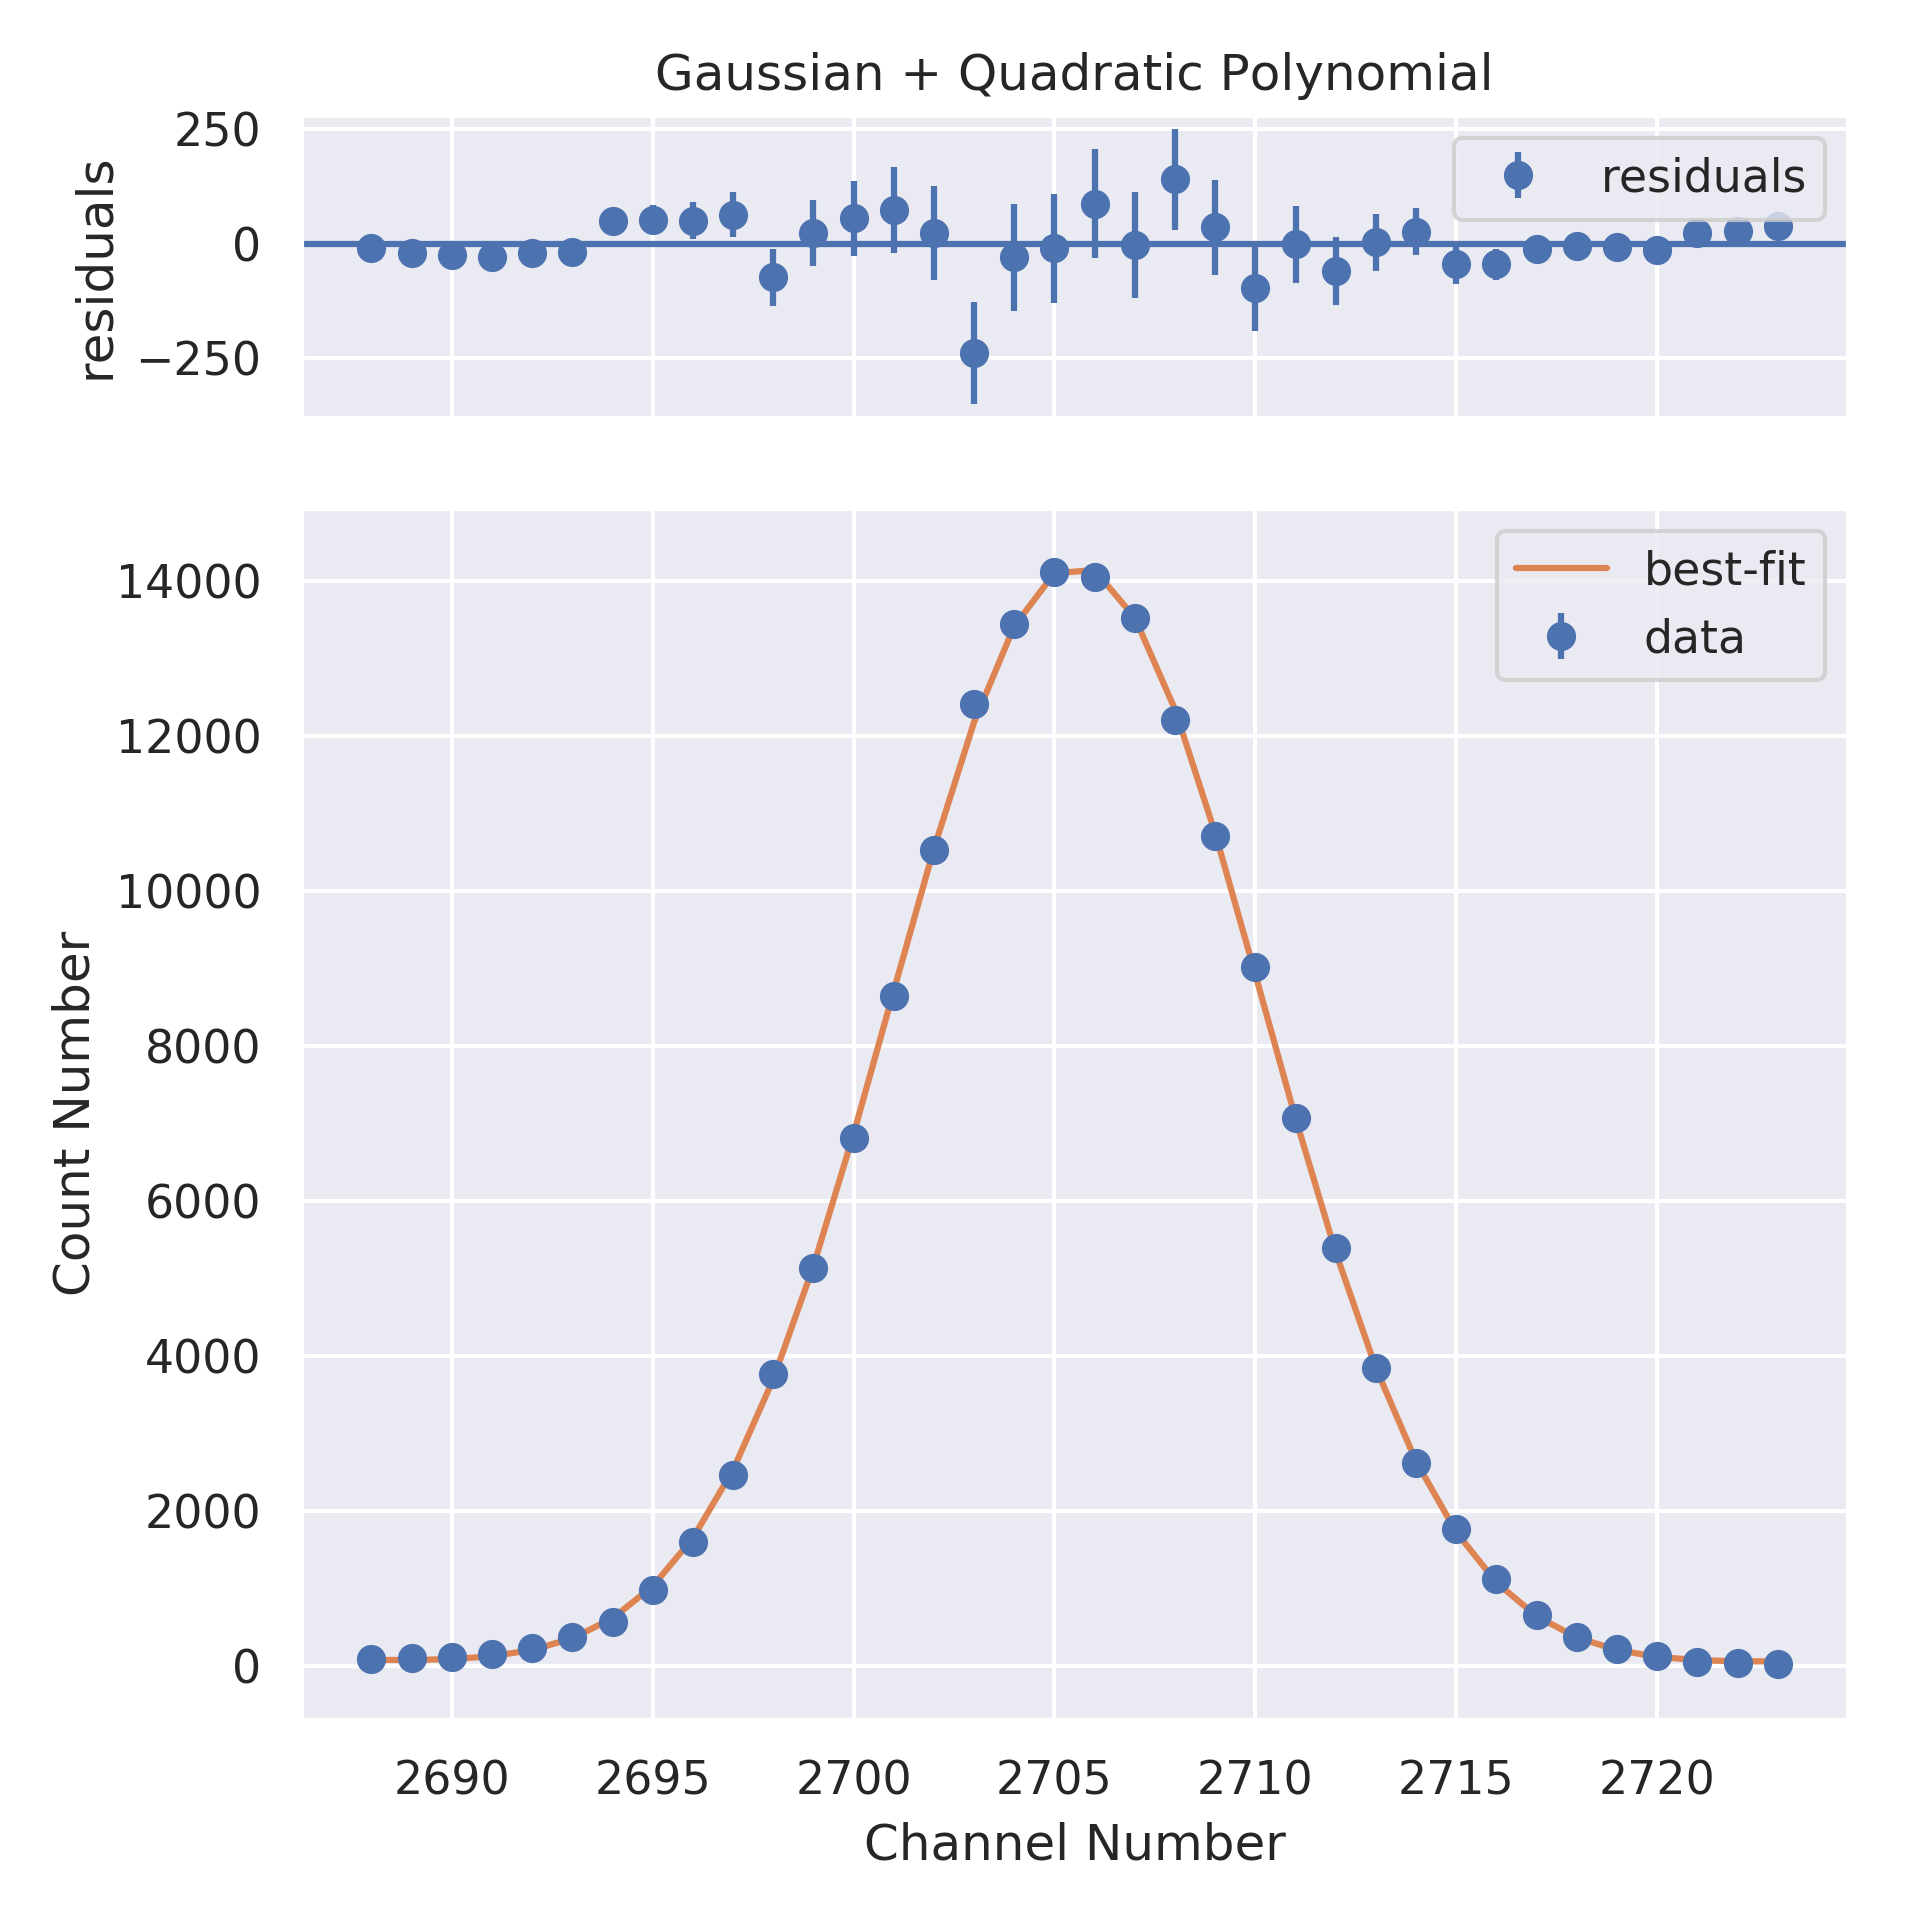
\includegraphics[width=\linewidth]{./Images/Barium133/Quad/Quad_7_Full.png}
    \caption{Full peak with fit}
    %\label{fig:sub1}
  \end{subfigure}%
  \begin{subfigure}{.5\linewidth}
    \centering
    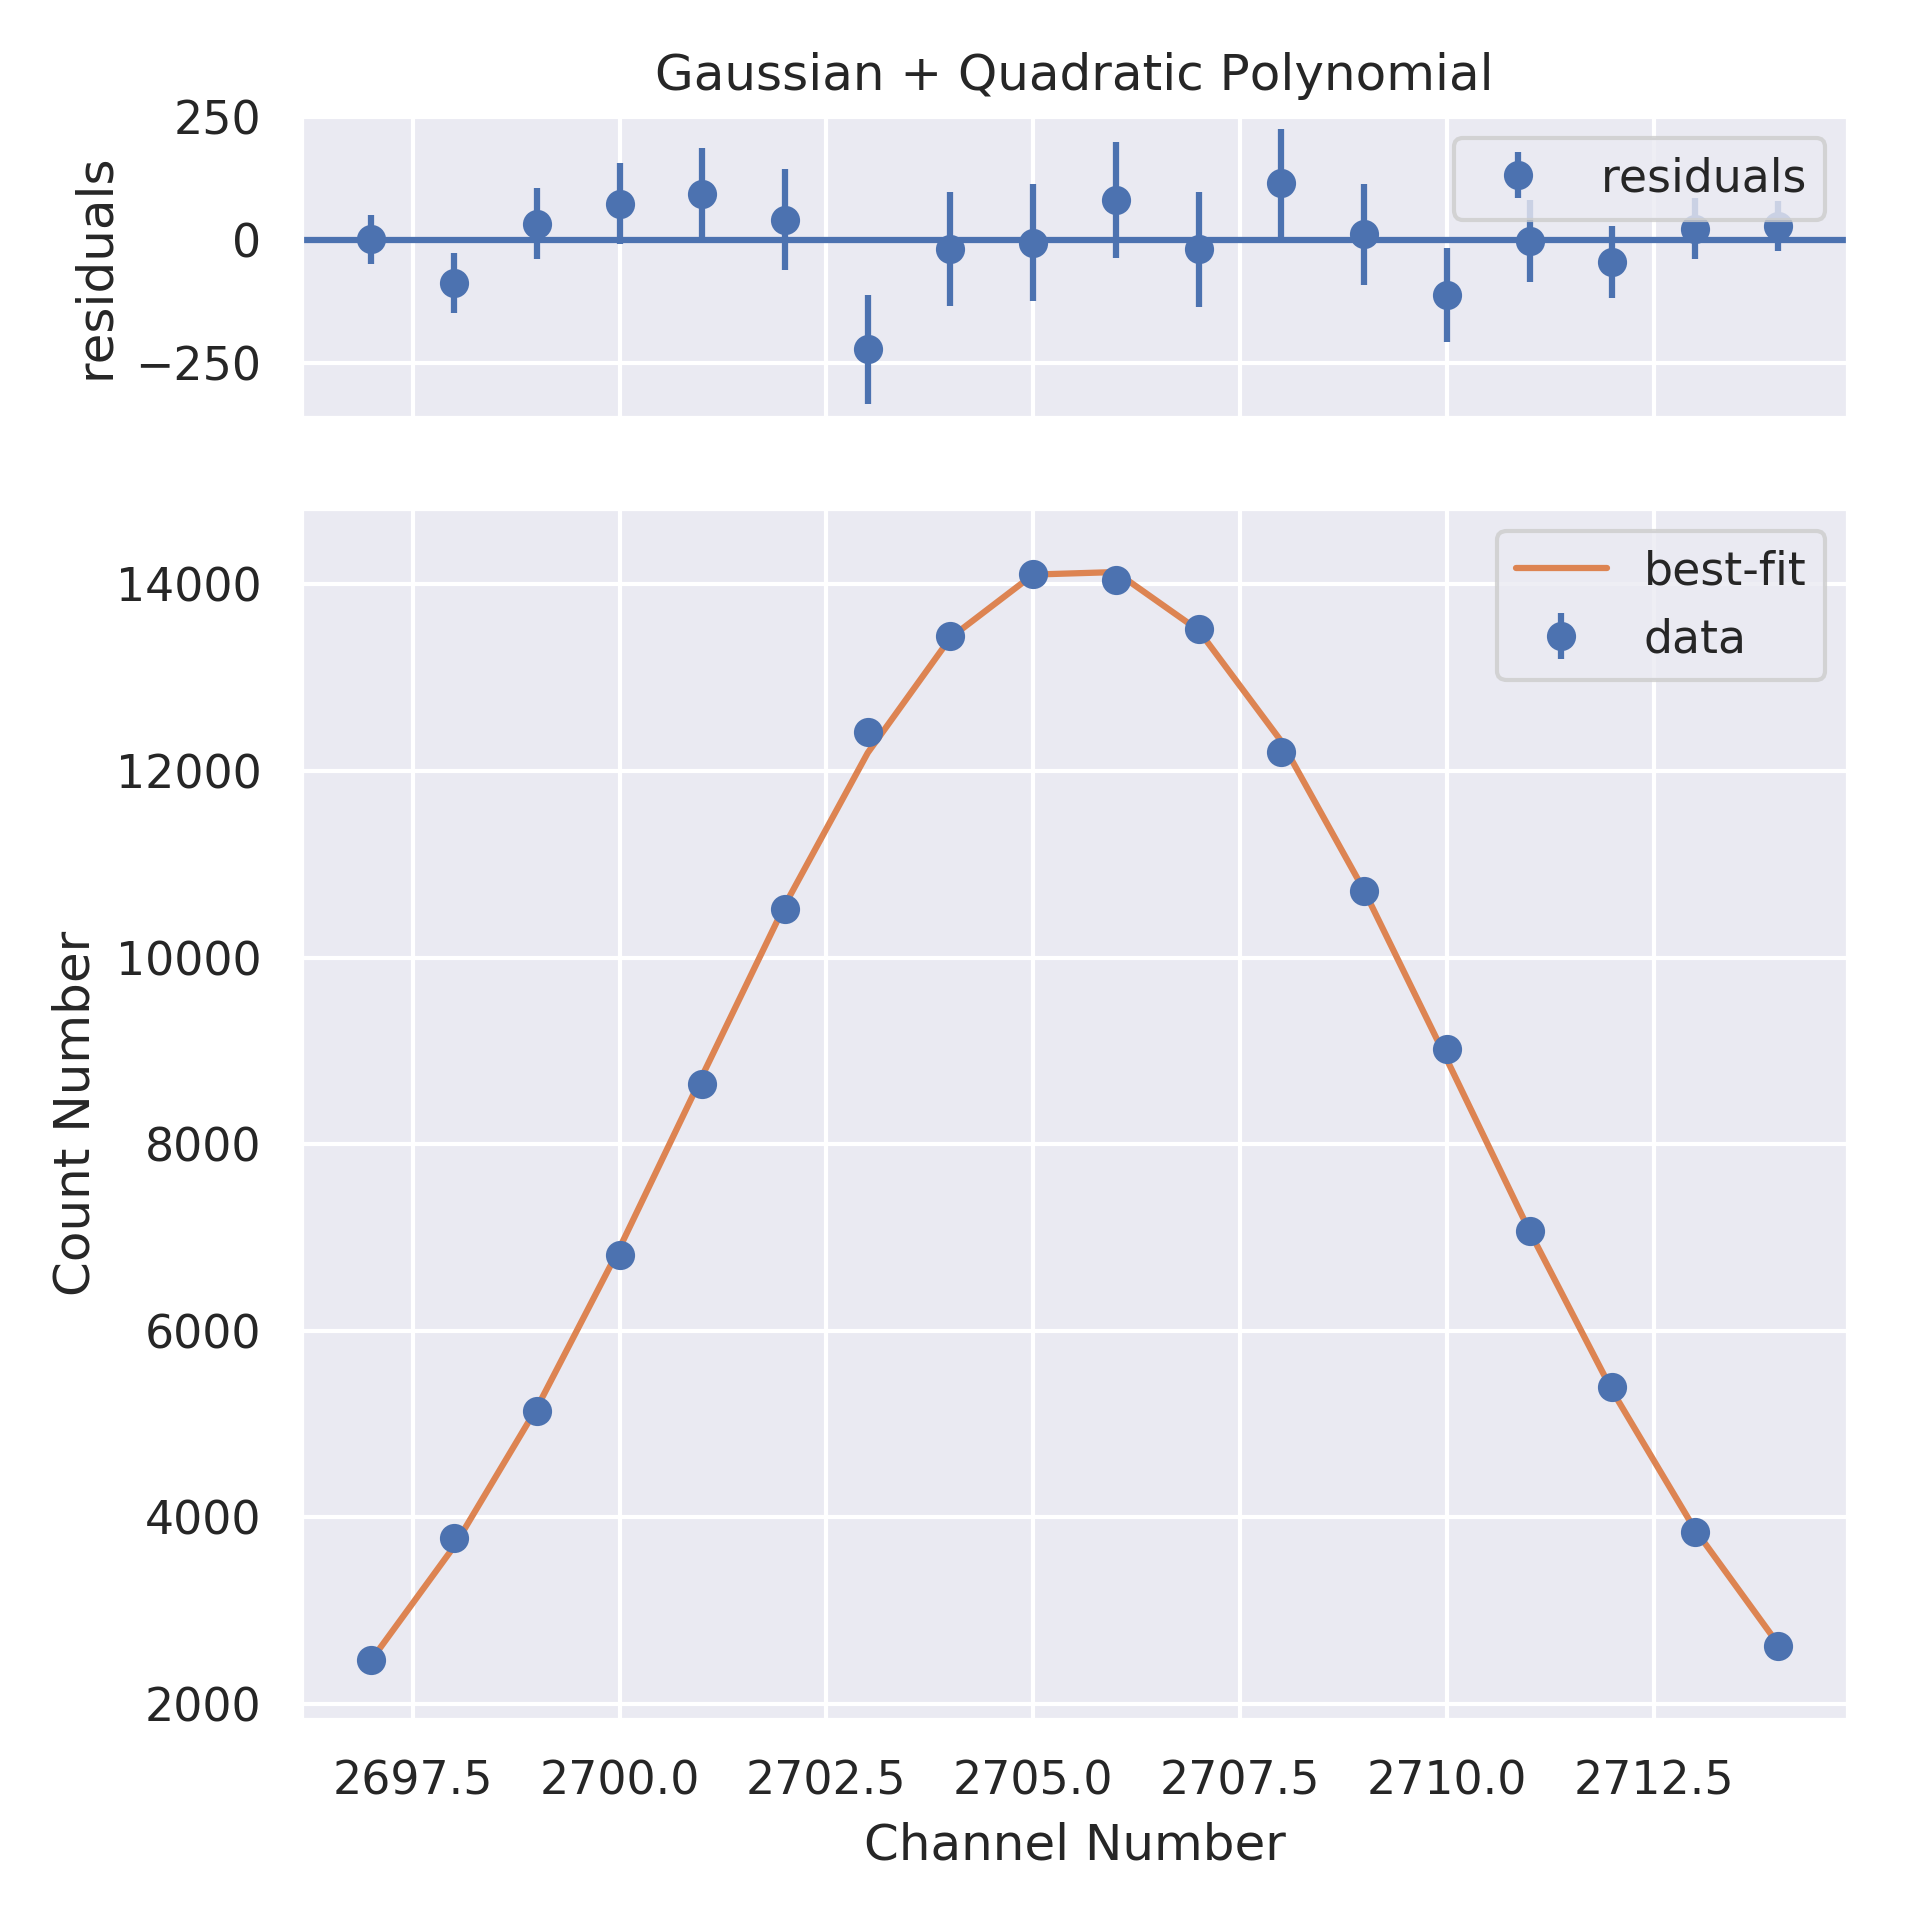
\includegraphics[width=\linewidth]{./Images/Barium133/Quad/Quad_7_Zoom.png}
    \caption{Zoomed in peak with fit}
    %\label{fig:sub2}
  \end{subfigure}
  \caption{Fit of full \& zoomed in peak of \element{Ba}{133} 384 keV peak}
  %\label{fig:test}
\end{figure}
\clearpage
\subsection{Cobalt-60}
\subsubsection{Gaussian Fit Only}
\begin{figure}[H]
  \centering
  \begin{subfigure}{.5\linewidth}
    \centering
    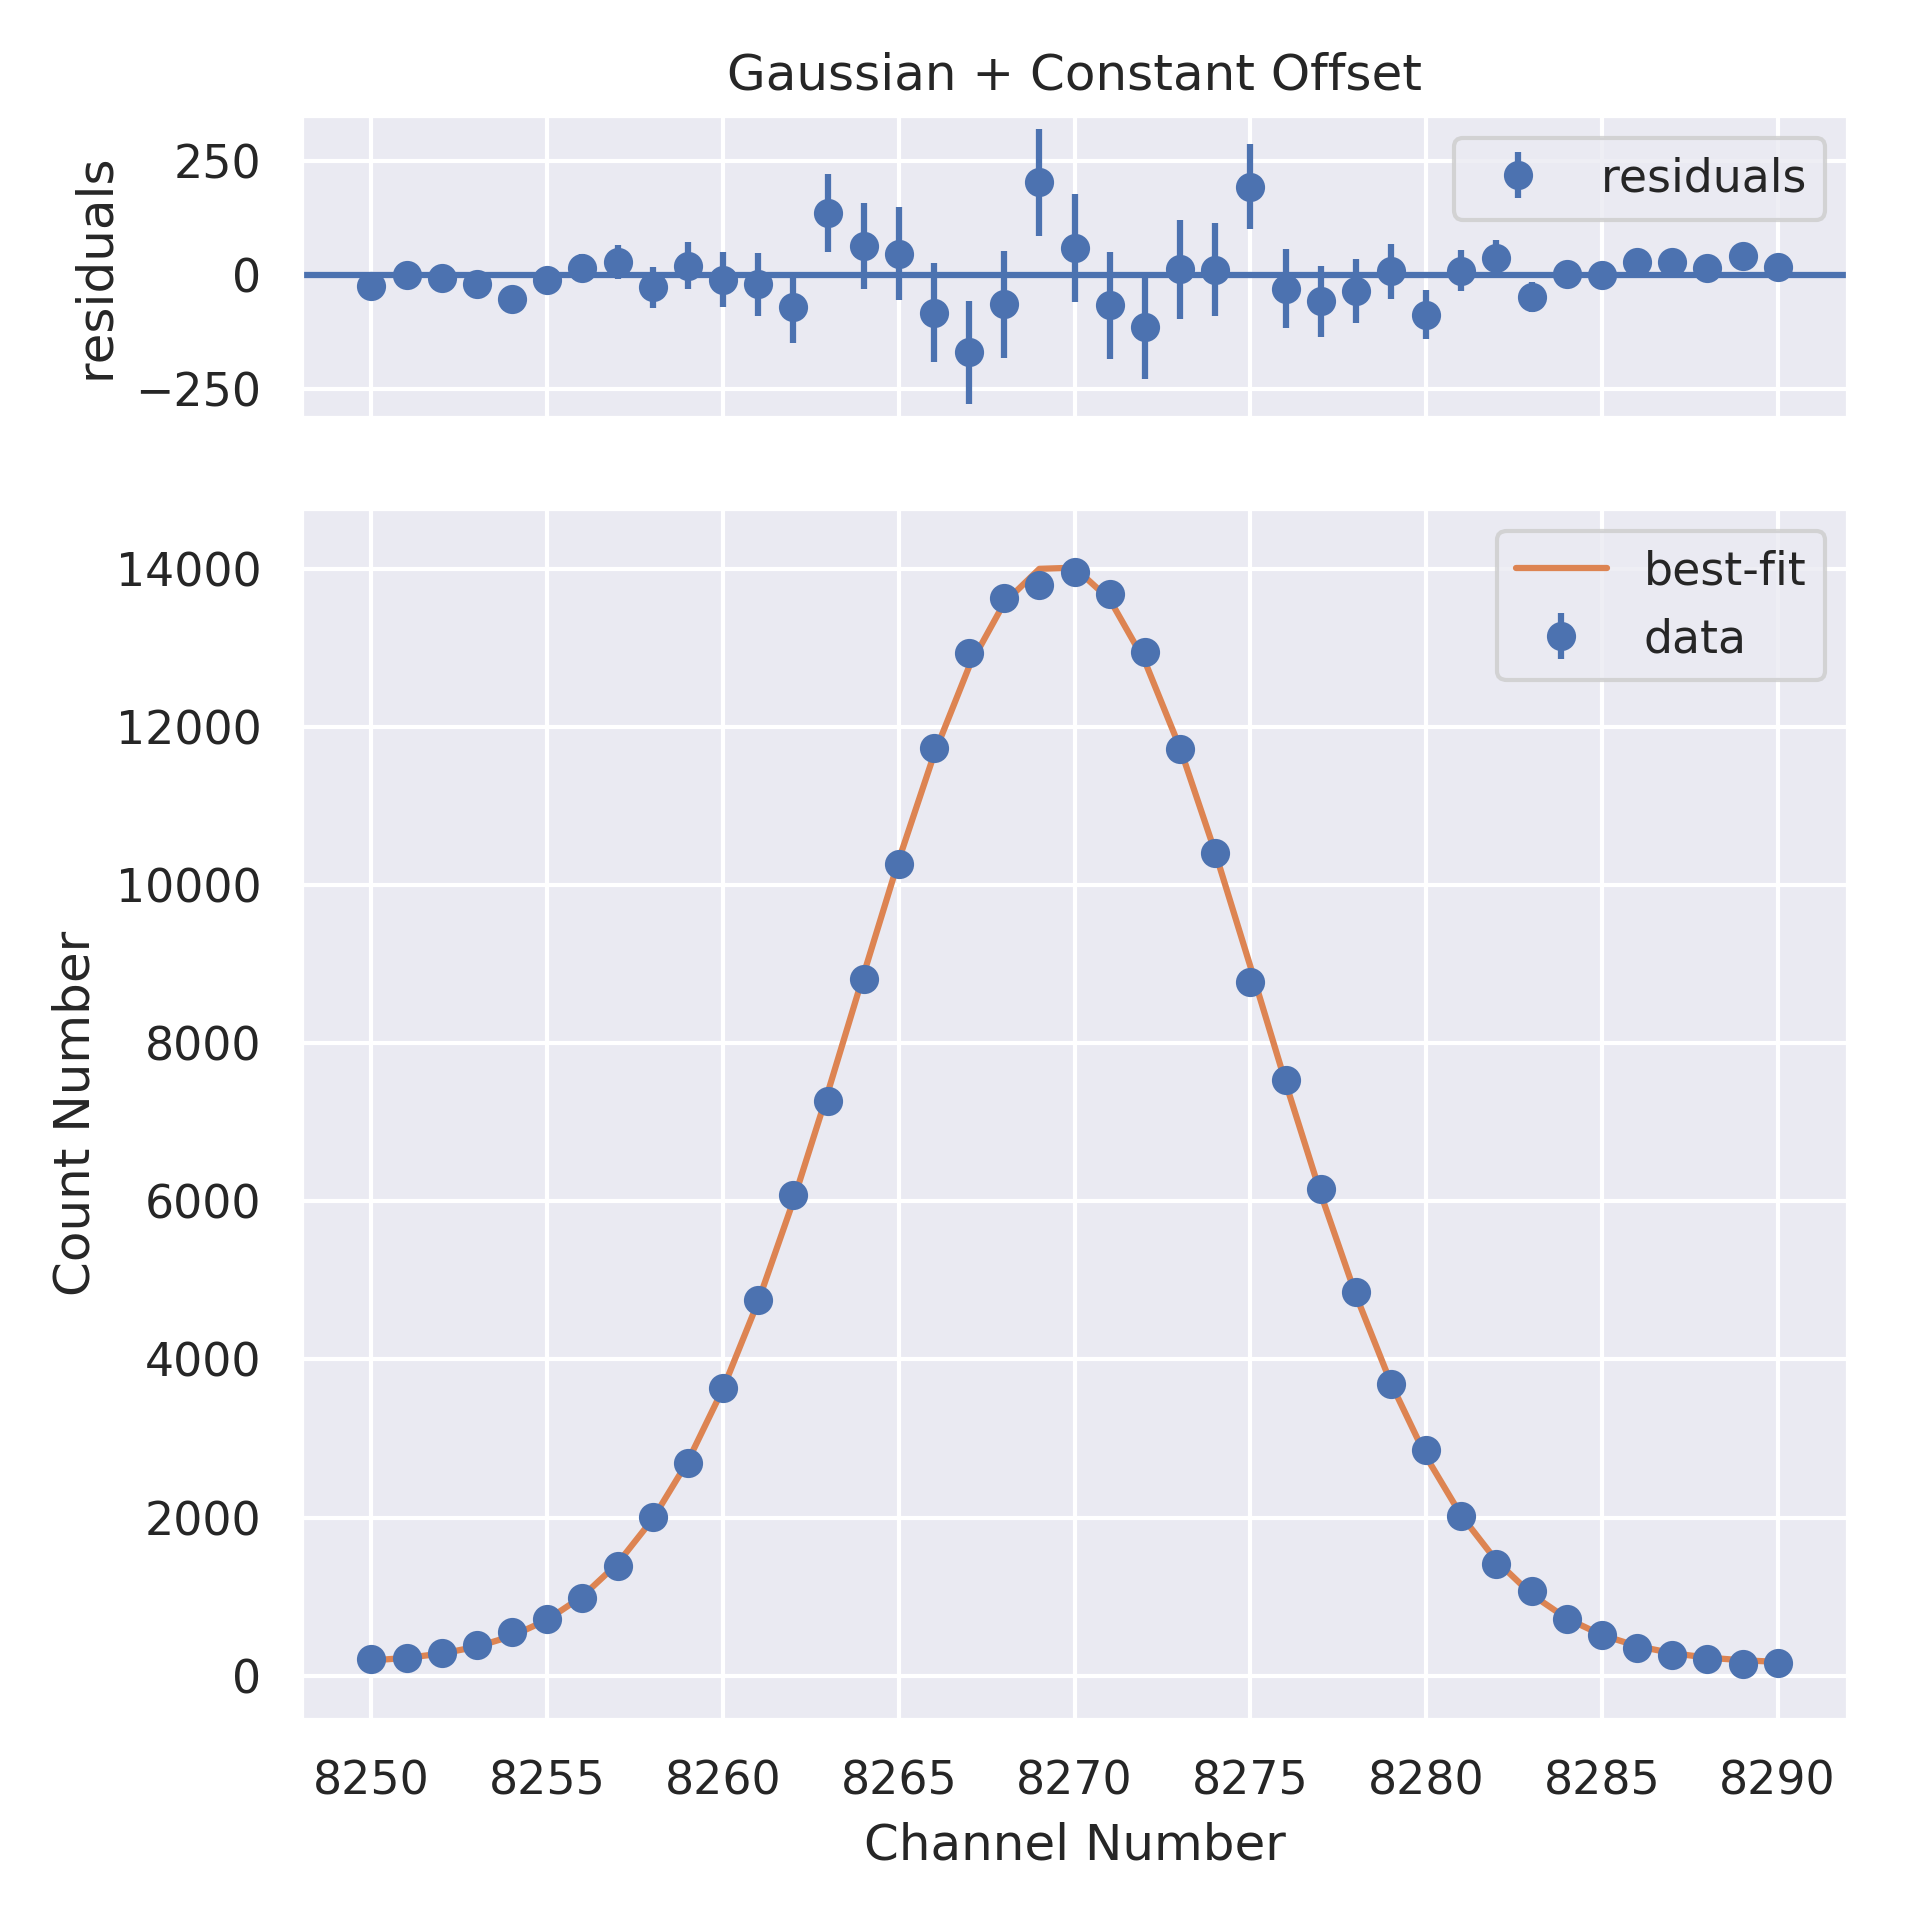
\includegraphics[width=\linewidth]{./Images/Cobalt60/Gauss/Gauss_1_Full.png}
    \caption{Full peak with fit}
    %\label{fig:sub1}
  \end{subfigure}%
  \begin{subfigure}{.5\linewidth}
    \centering
    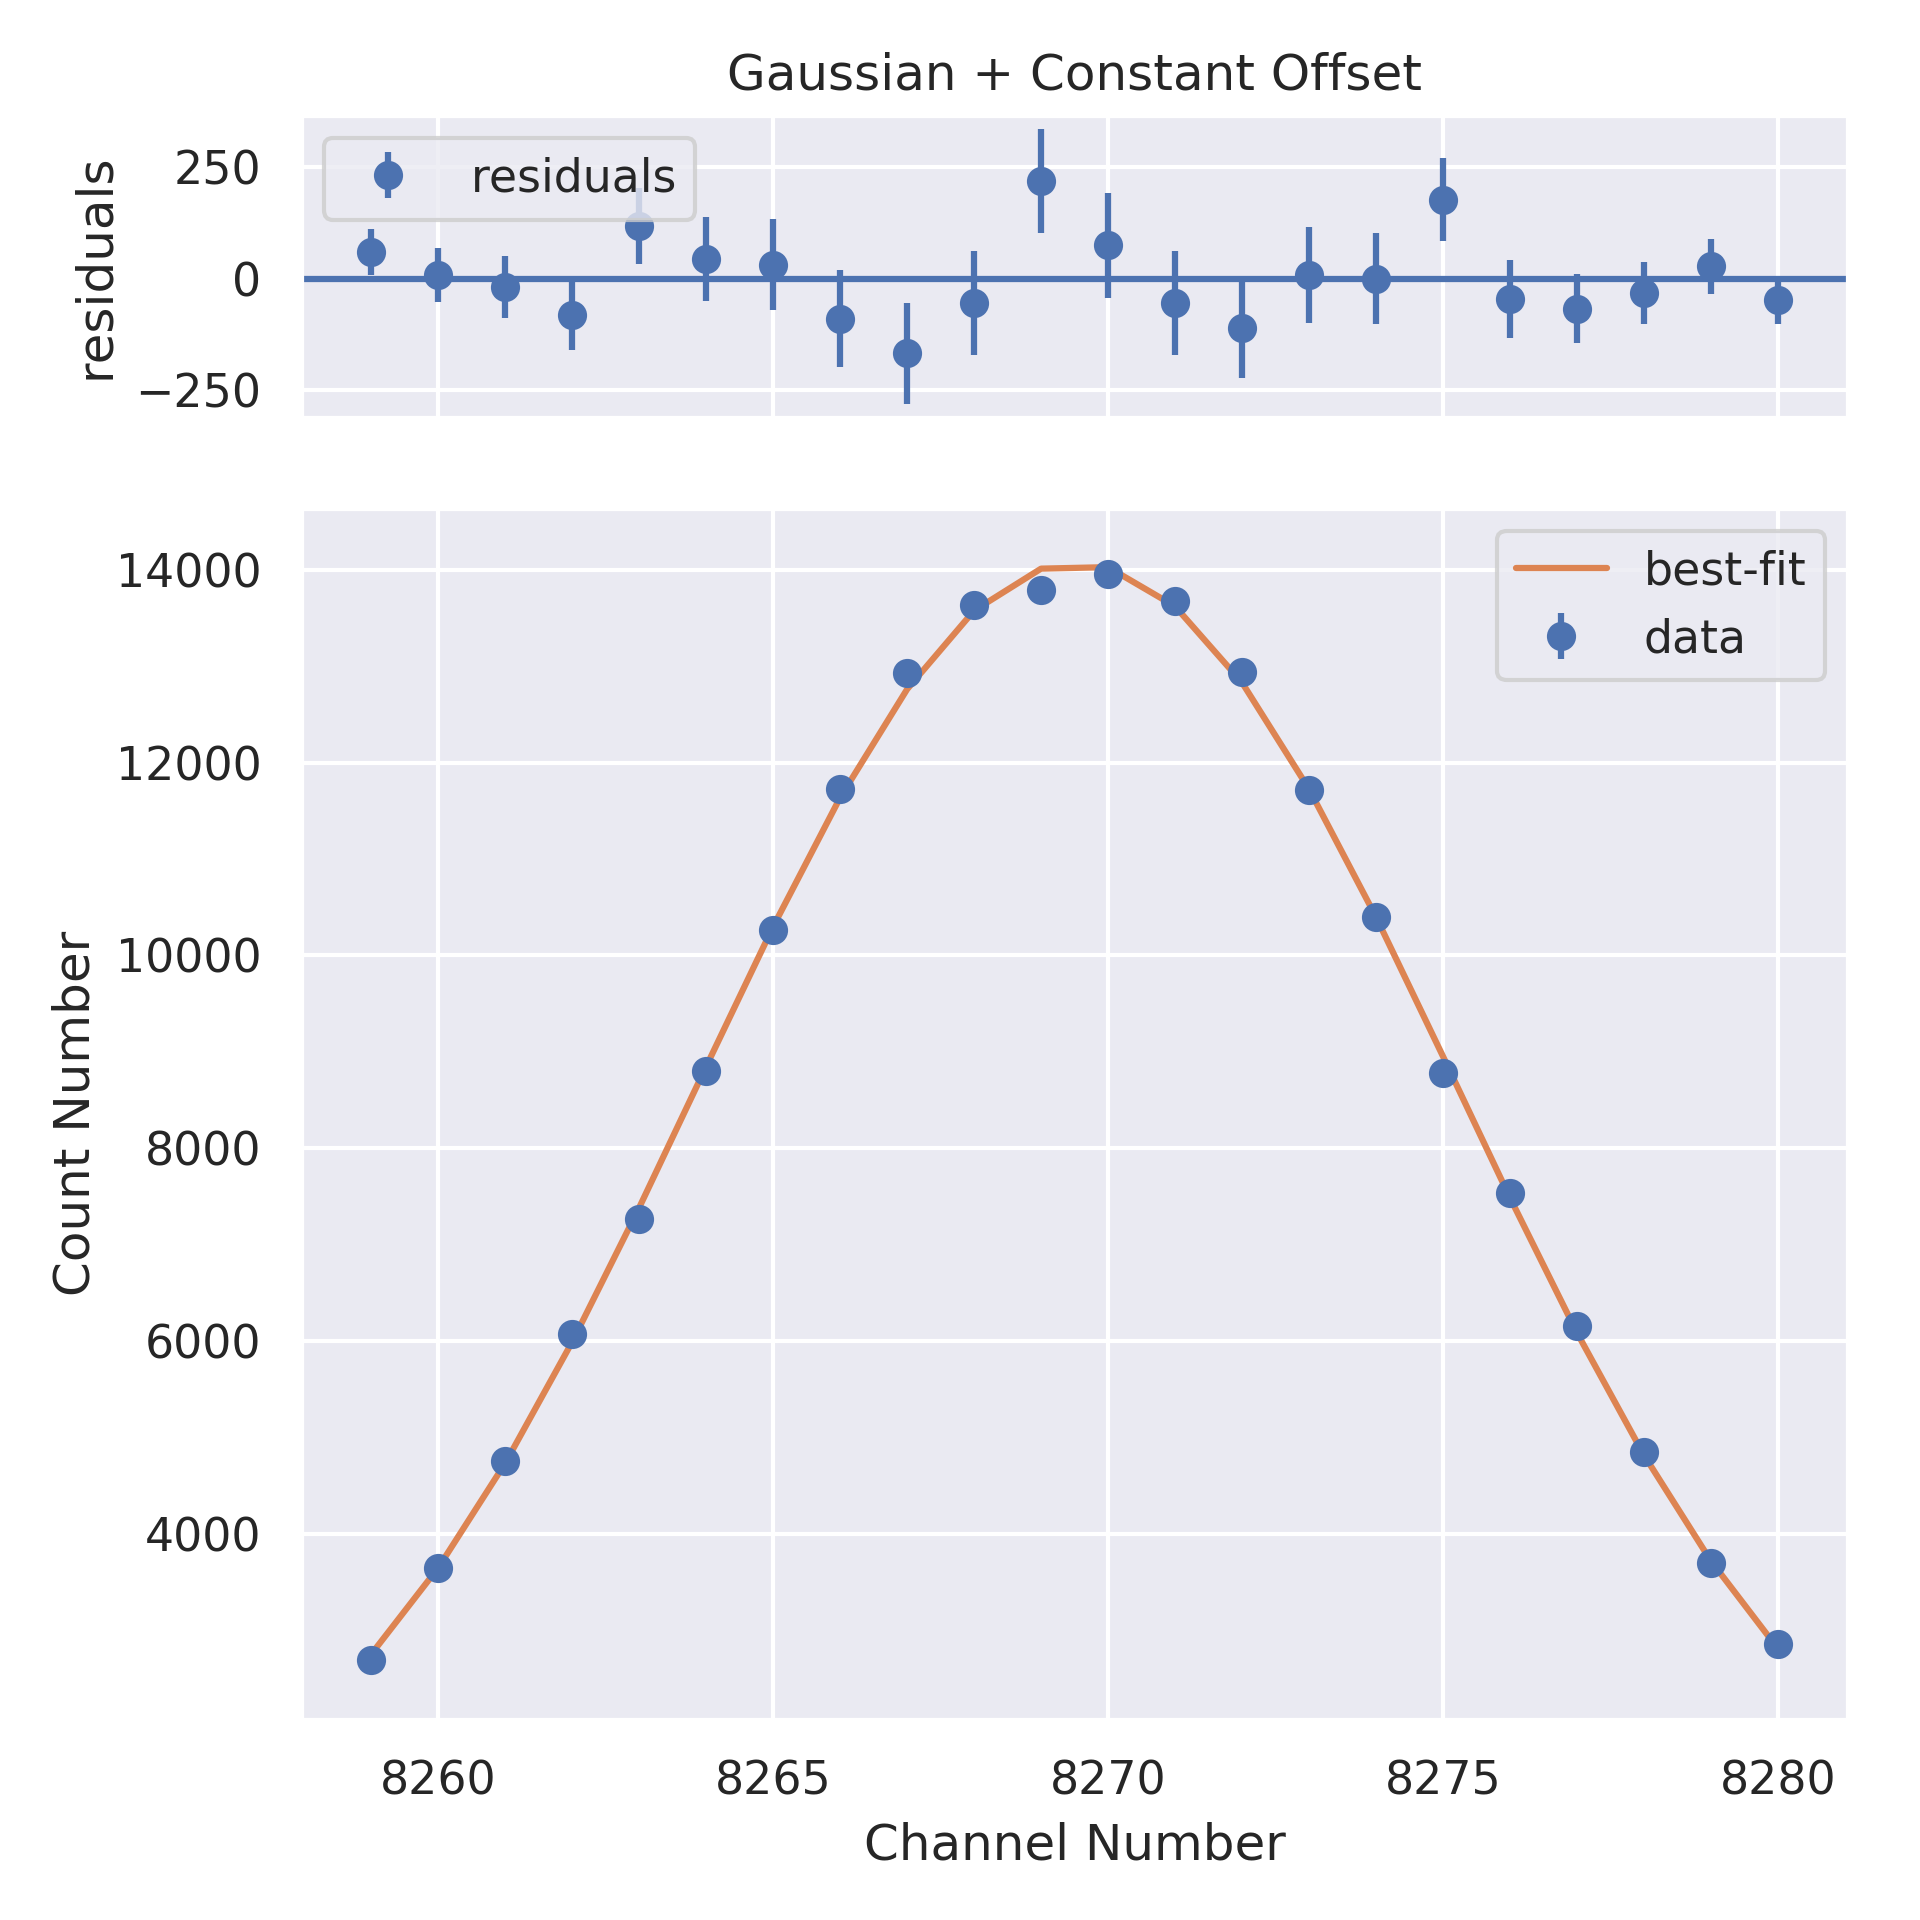
\includegraphics[width=\linewidth]{./Images/Cobalt60/Gauss/Gauss_1_Zoom.png}
    \caption{Zoomed in peak with fit}
    %\label{fig:sub2}
  \end{subfigure}
  \caption{Fit of full \& zoomed in peak of \element{Co}{60} 1173 keV peak}
  %\label{fig:test}
\end{figure}
\begin{figure}[H]
  \centering
  \begin{subfigure}{.5\linewidth}
    \centering
    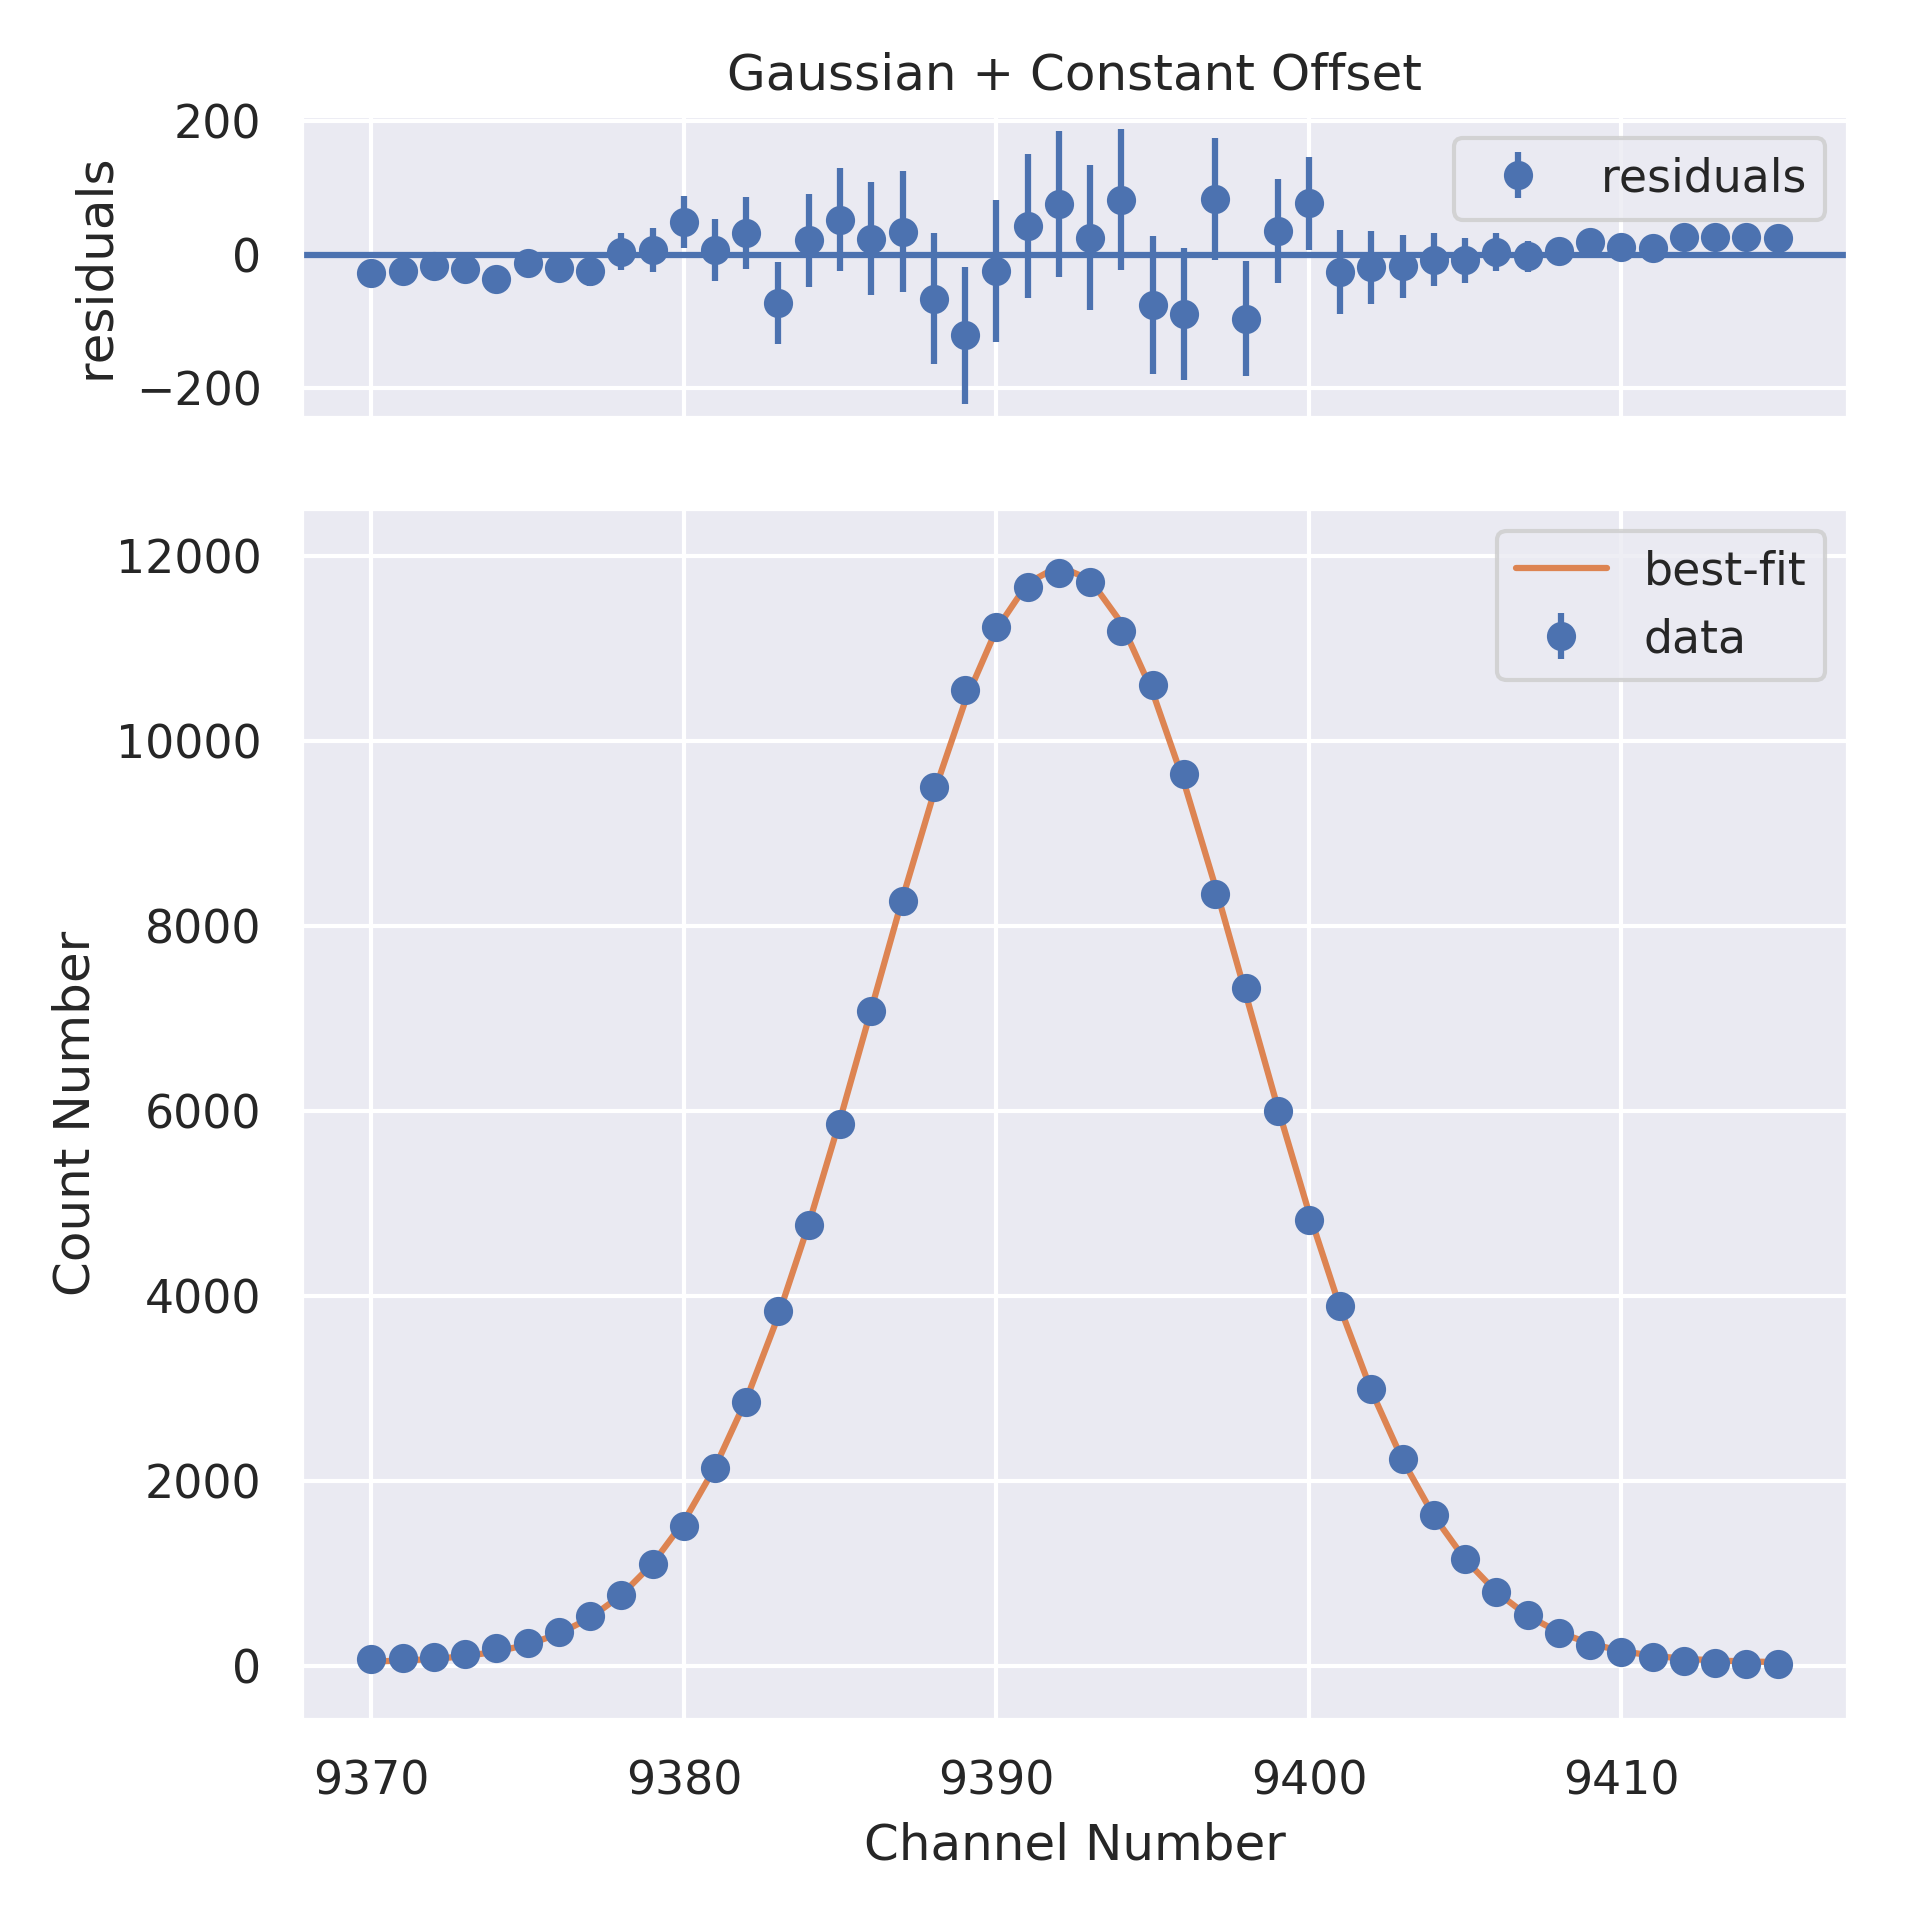
\includegraphics[width=\linewidth]{./Images/Cobalt60/Gauss/Gauss_2_Full.png}
    \caption{Full peak with fit}
    %\label{fig:sub1}
  \end{subfigure}%
  \begin{subfigure}{.5\linewidth}
    \centering
    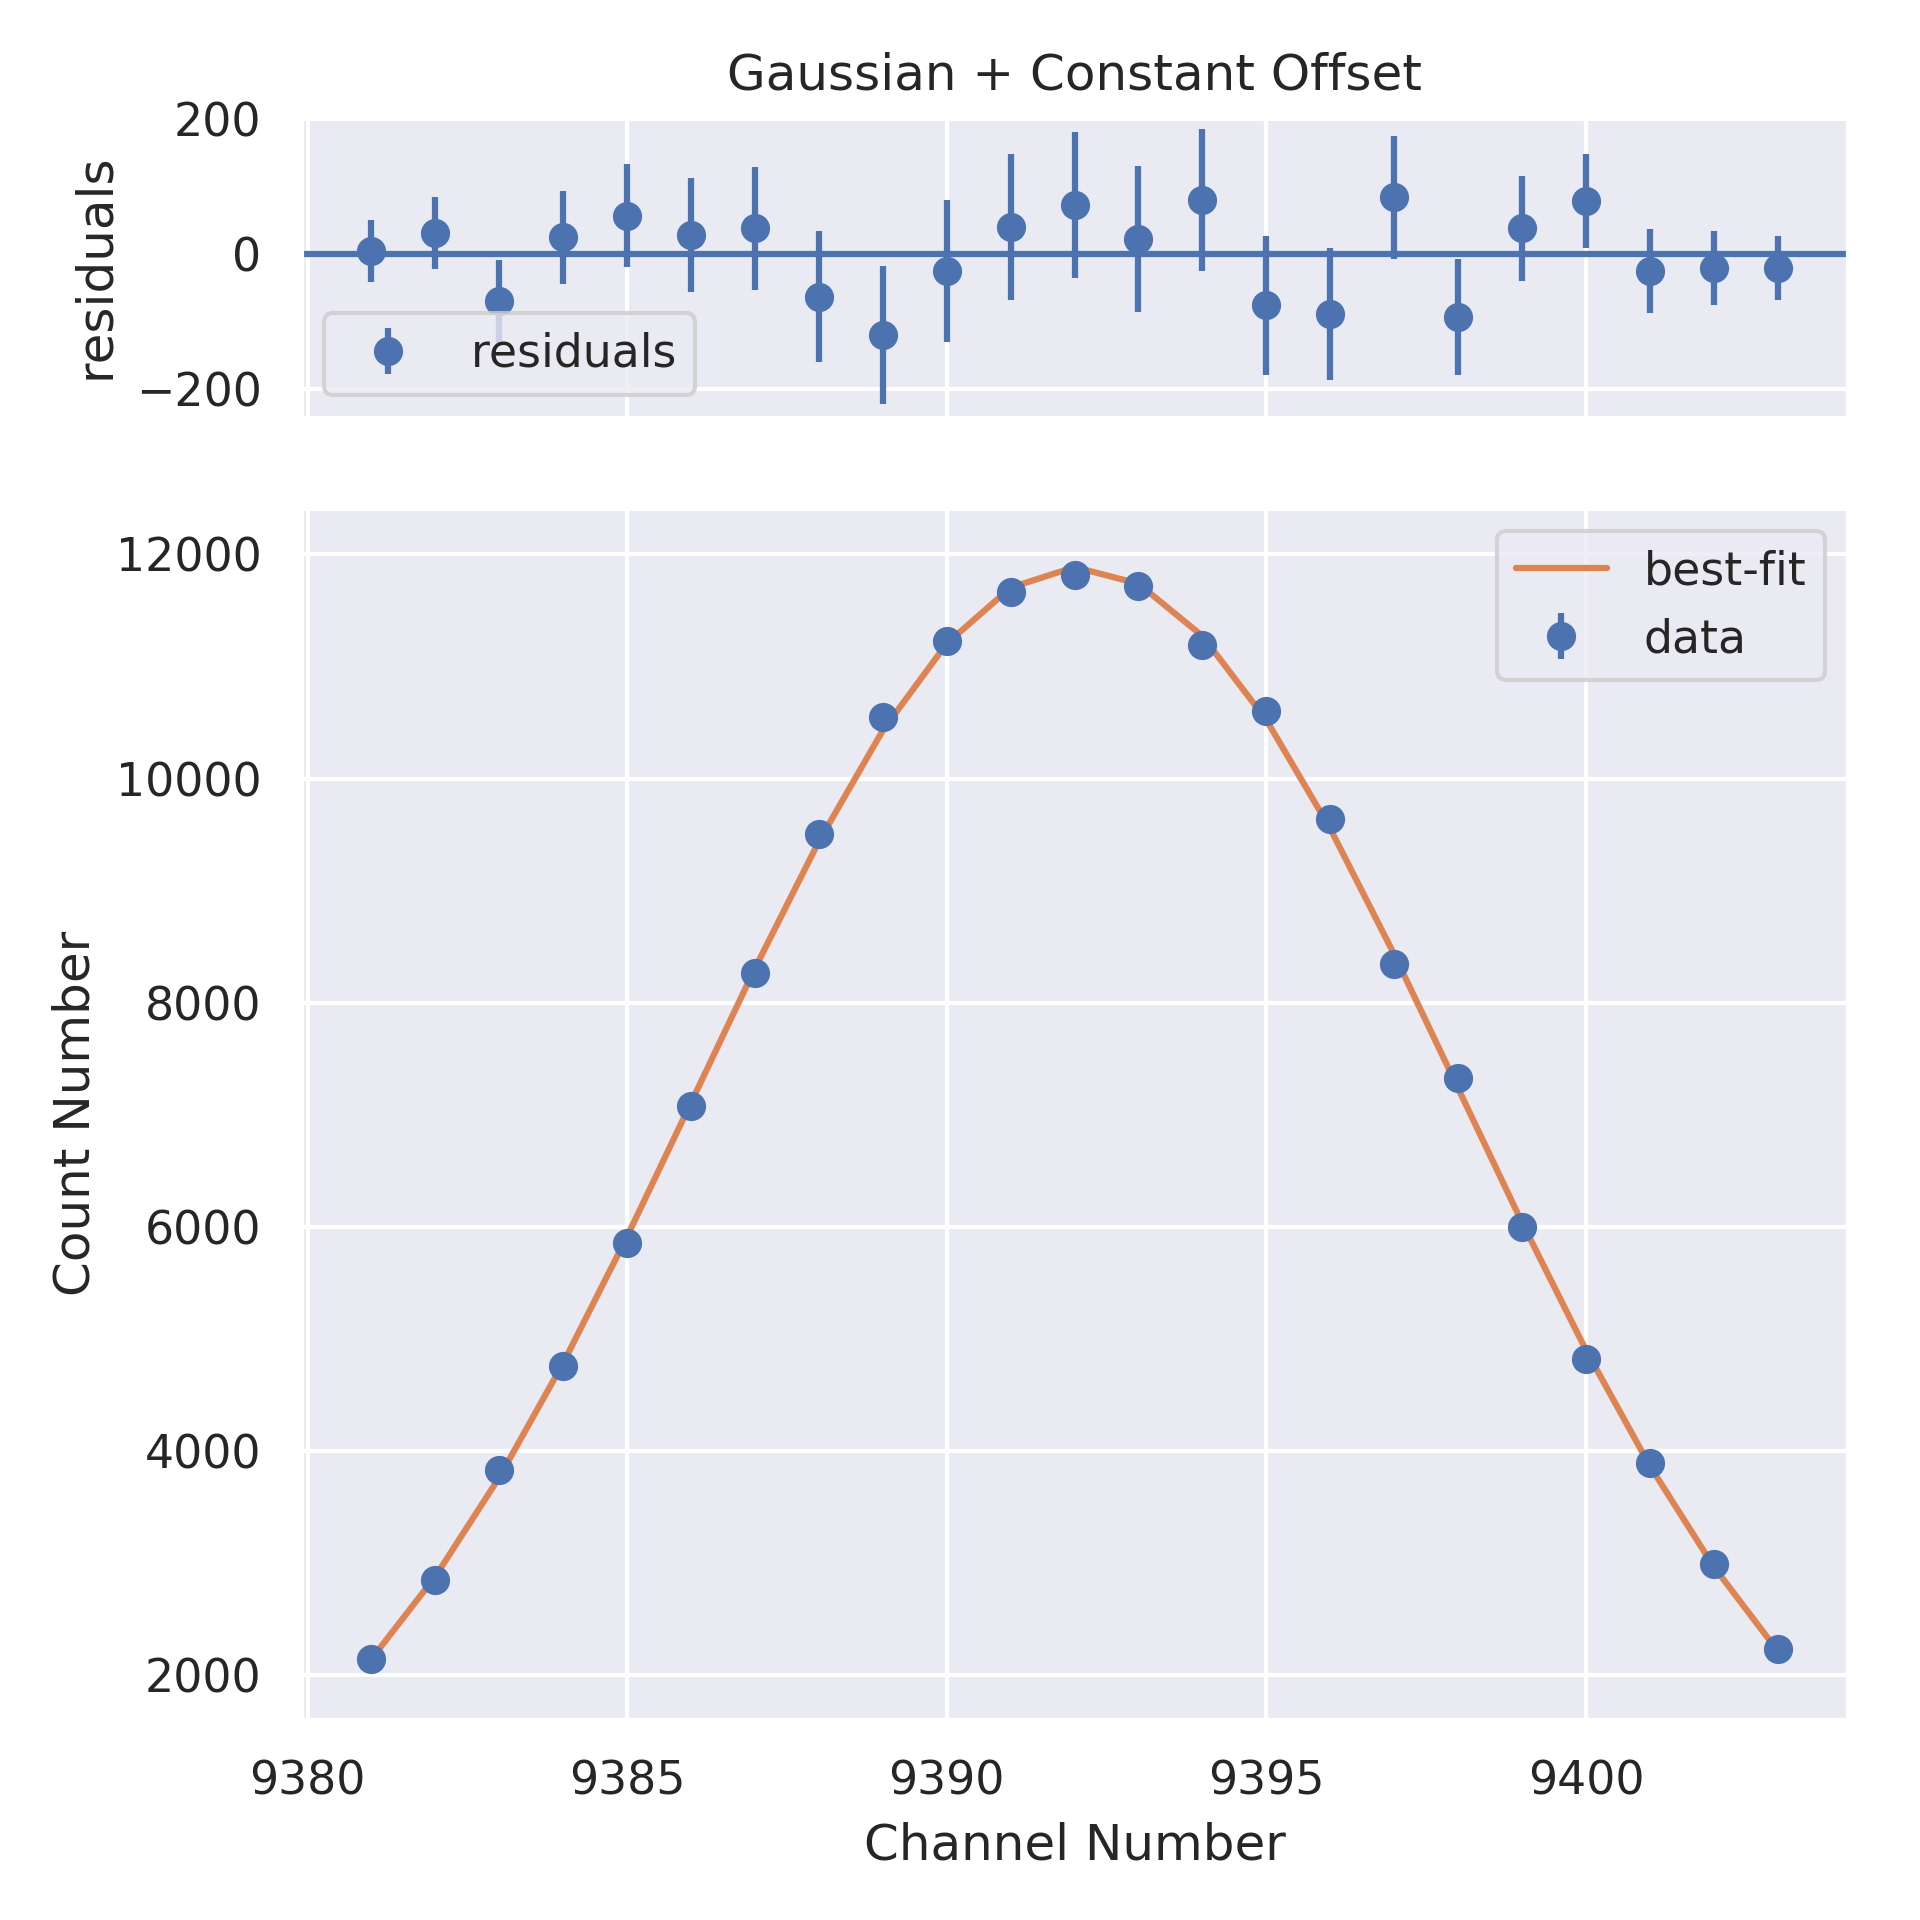
\includegraphics[width=\linewidth]{./Images/Cobalt60/Gauss/Gauss_2_Zoom.png}
    \caption{Zoomed in peak with fit}
    %\label{fig:sub2}
  \end{subfigure}
  \caption{Fit of full \& zoomed in peak of \element{Co}{60} 1332 keV peak}
  %\label{fig:test}
\end{figure}
\clearpage
\subsubsection{Linear + Gaussian Fit}
\begin{figure}[H]
  \centering
  \begin{subfigure}{.5\linewidth}
    \centering
    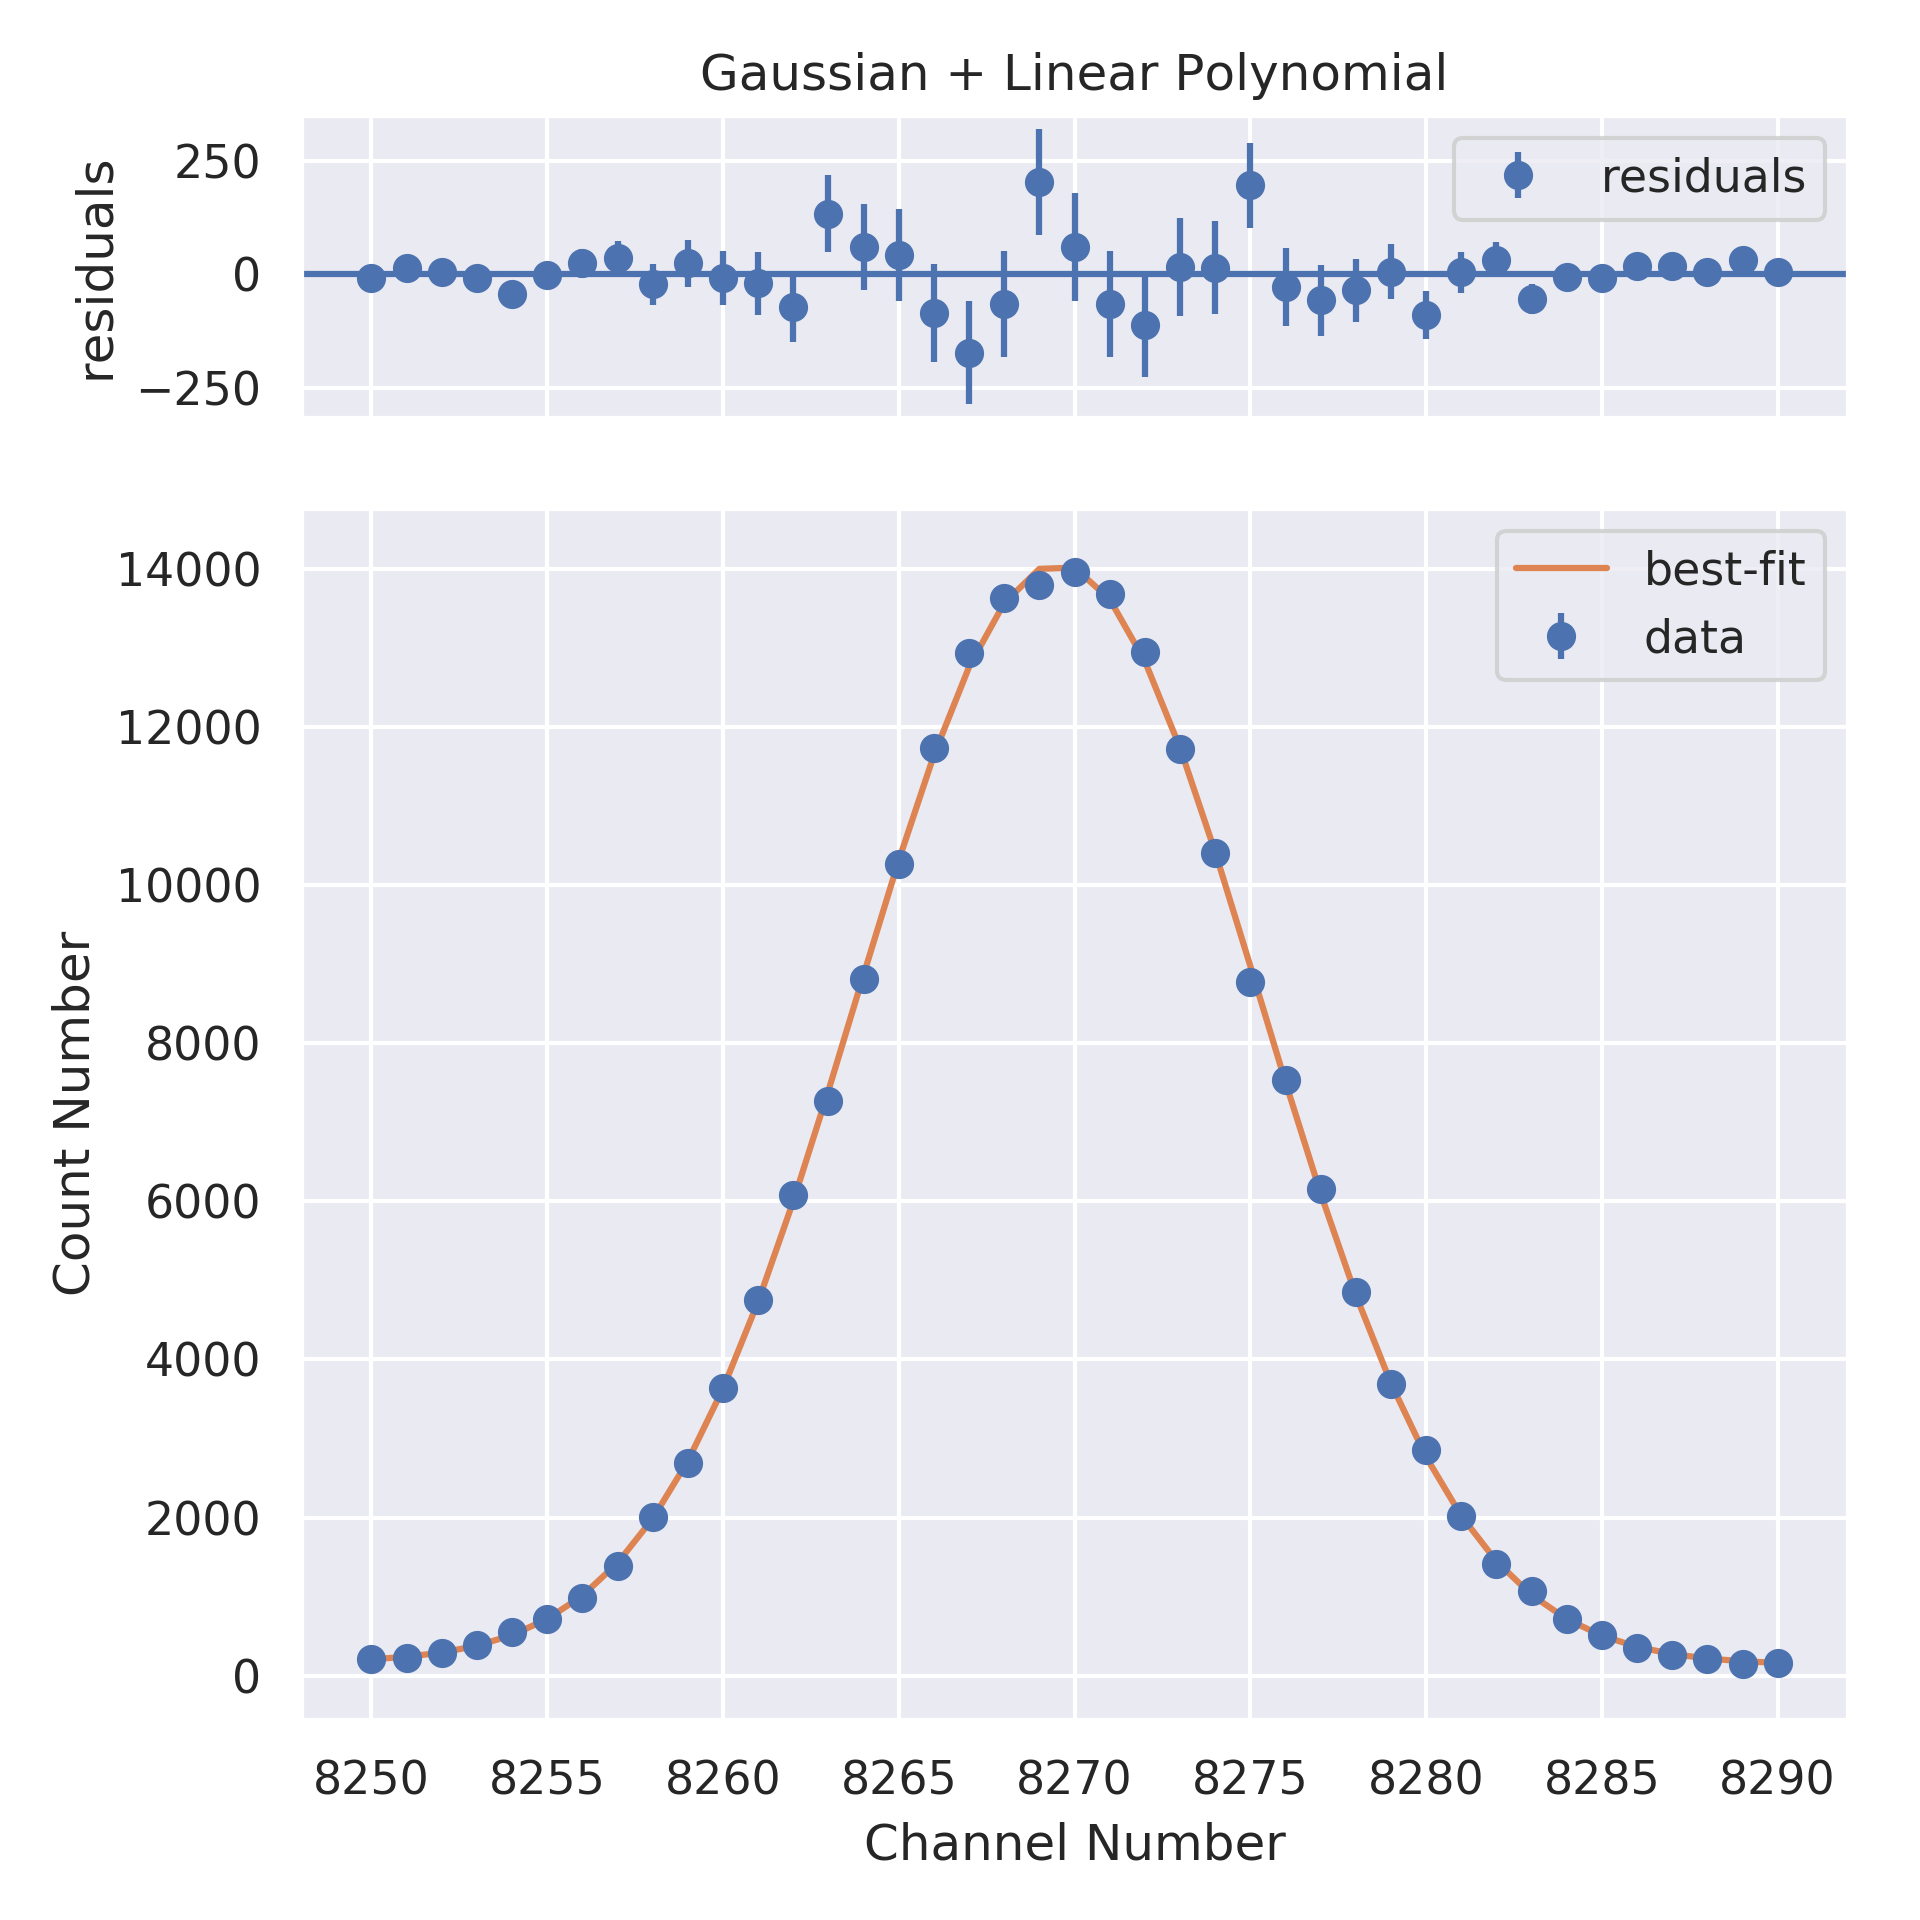
\includegraphics[width=\linewidth]{./Images/Cobalt60/Linear/Linear_1_Full.png}
    \caption{Full peak with fit}
    %\label{fig:sub1}
  \end{subfigure}%
  \begin{subfigure}{.5\linewidth}
    \centering
    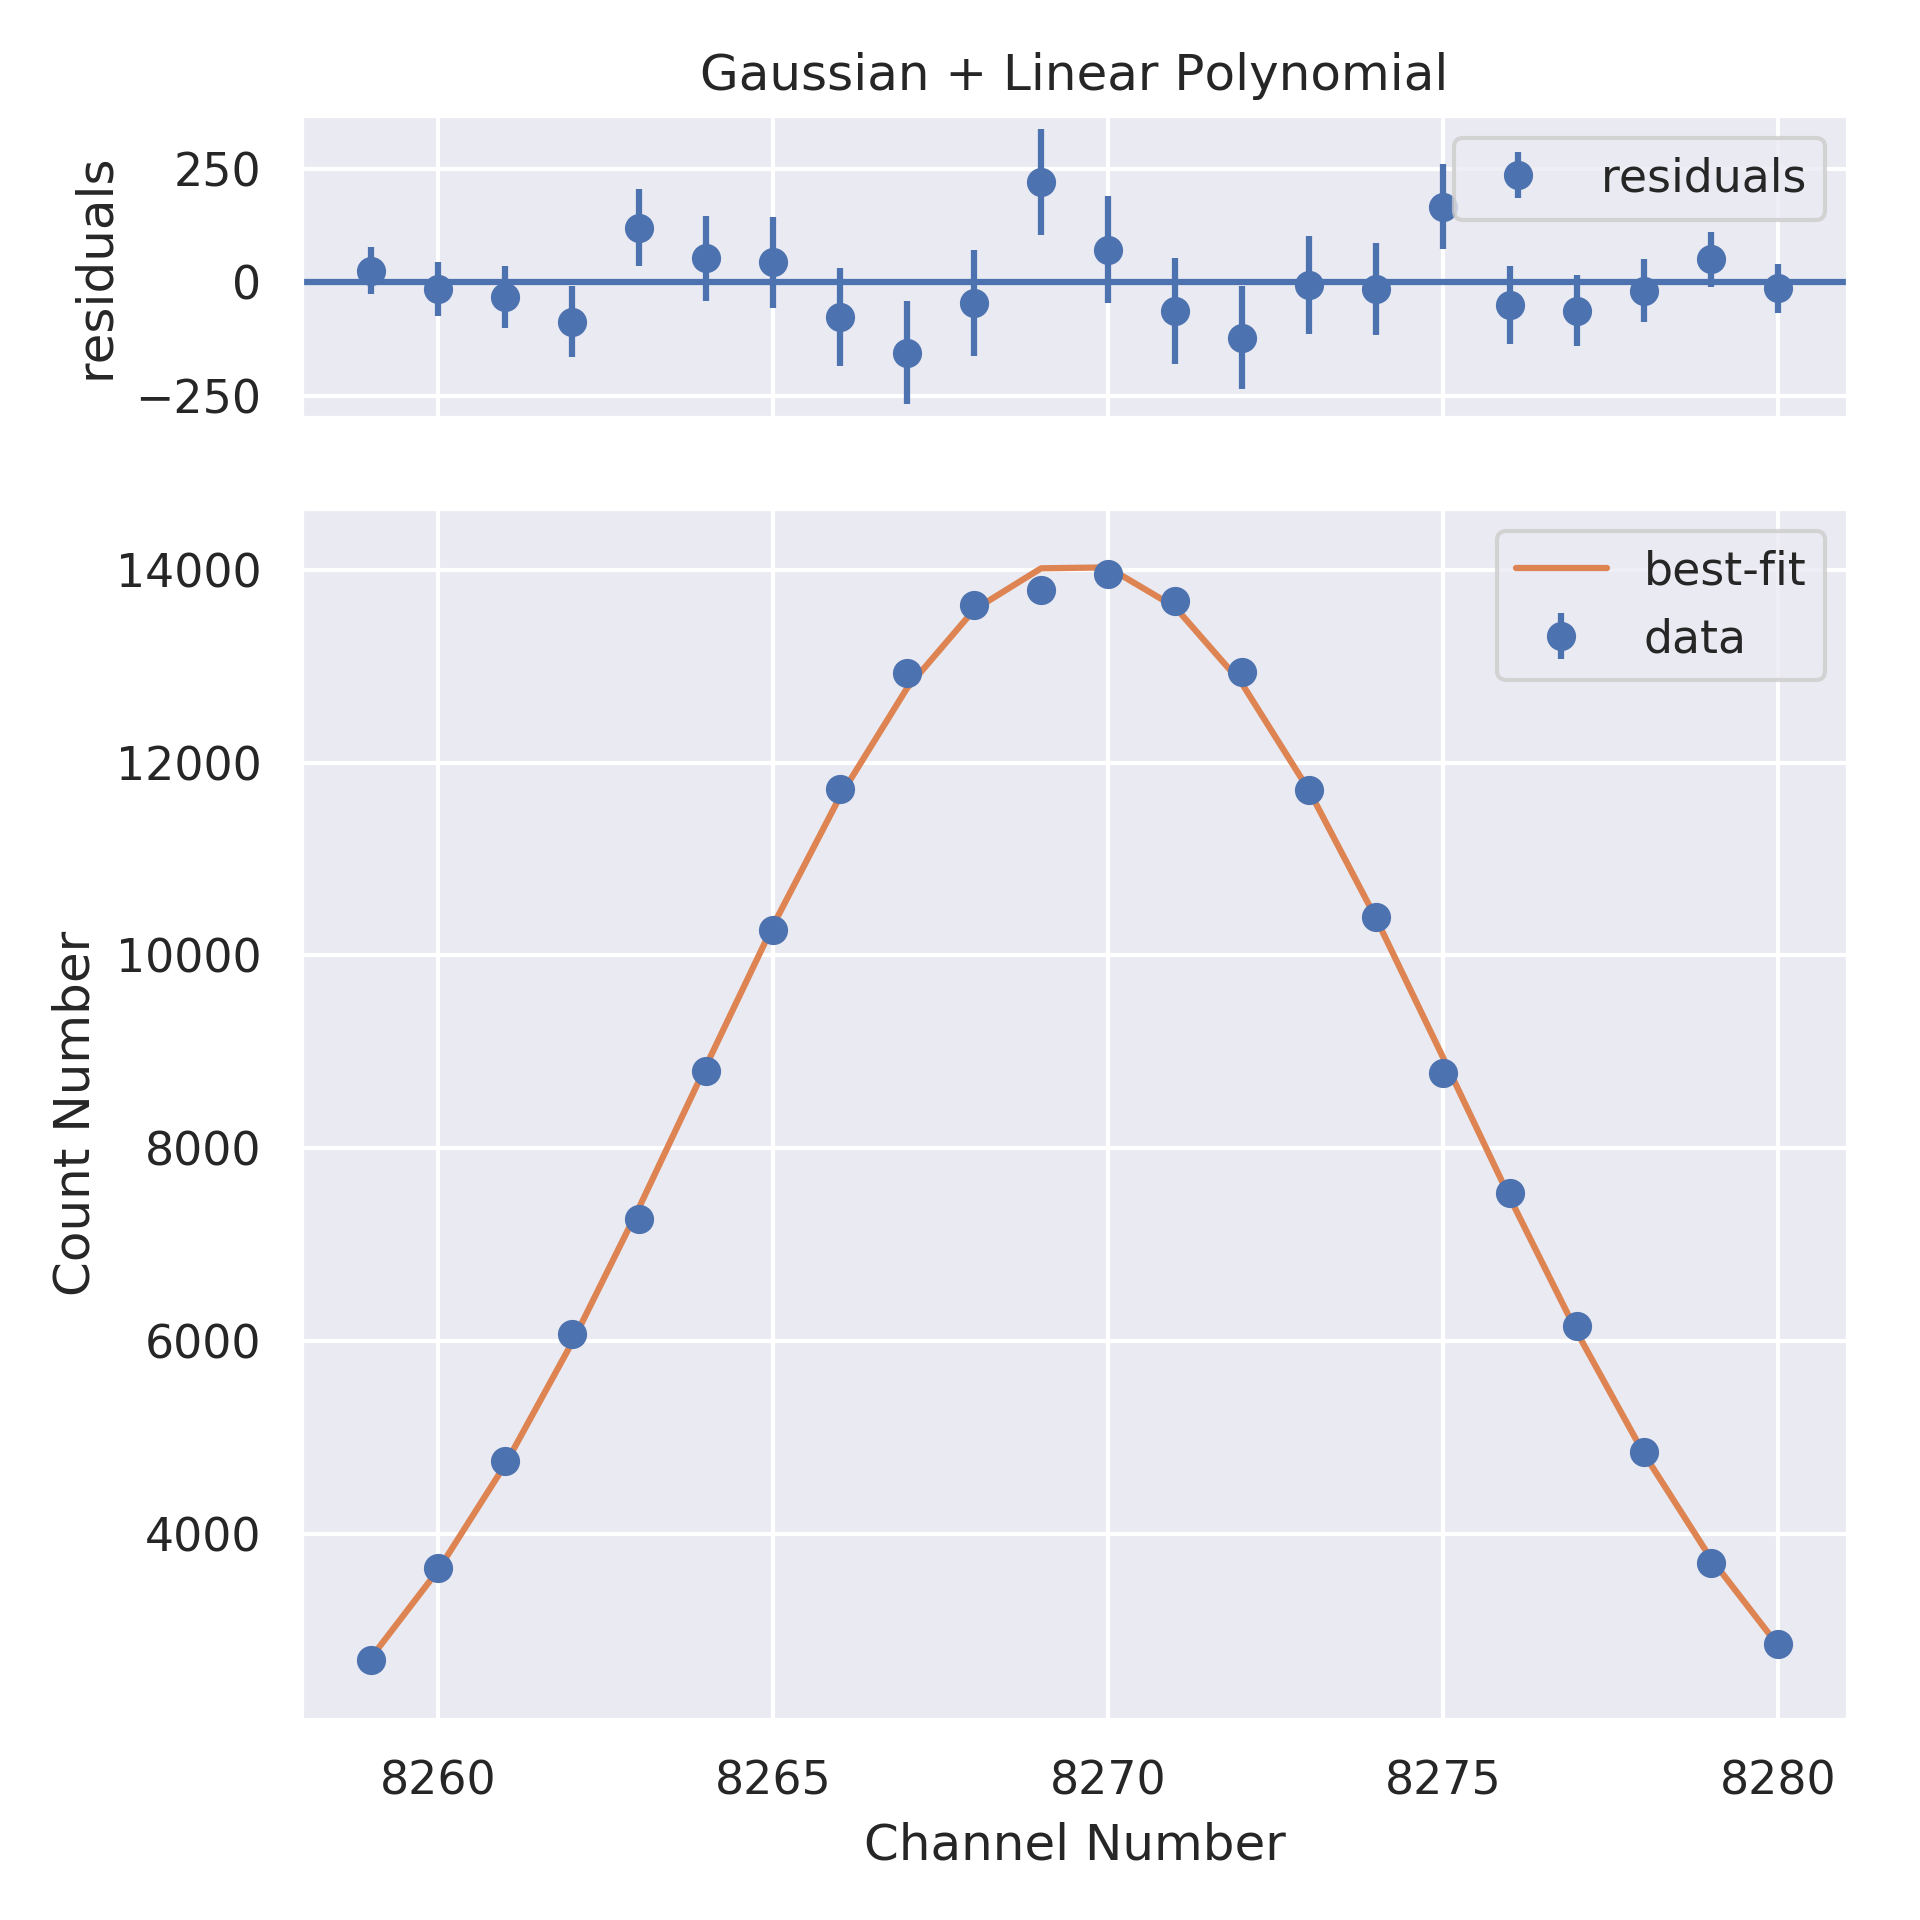
\includegraphics[width=\linewidth]{./Images/Cobalt60/Linear/Linear_1_Zoom.png}
    \caption{Zoomed in peak with fit}
    %\label{fig:sub2}
  \end{subfigure}
  \caption{Fit of full \& zoomed in peak of \element{Co}{60} 1173 keV peak}
  %\label{fig:test}
\end{figure}
\begin{figure}[H]
  \centering
  \begin{subfigure}{.5\linewidth}
    \centering
    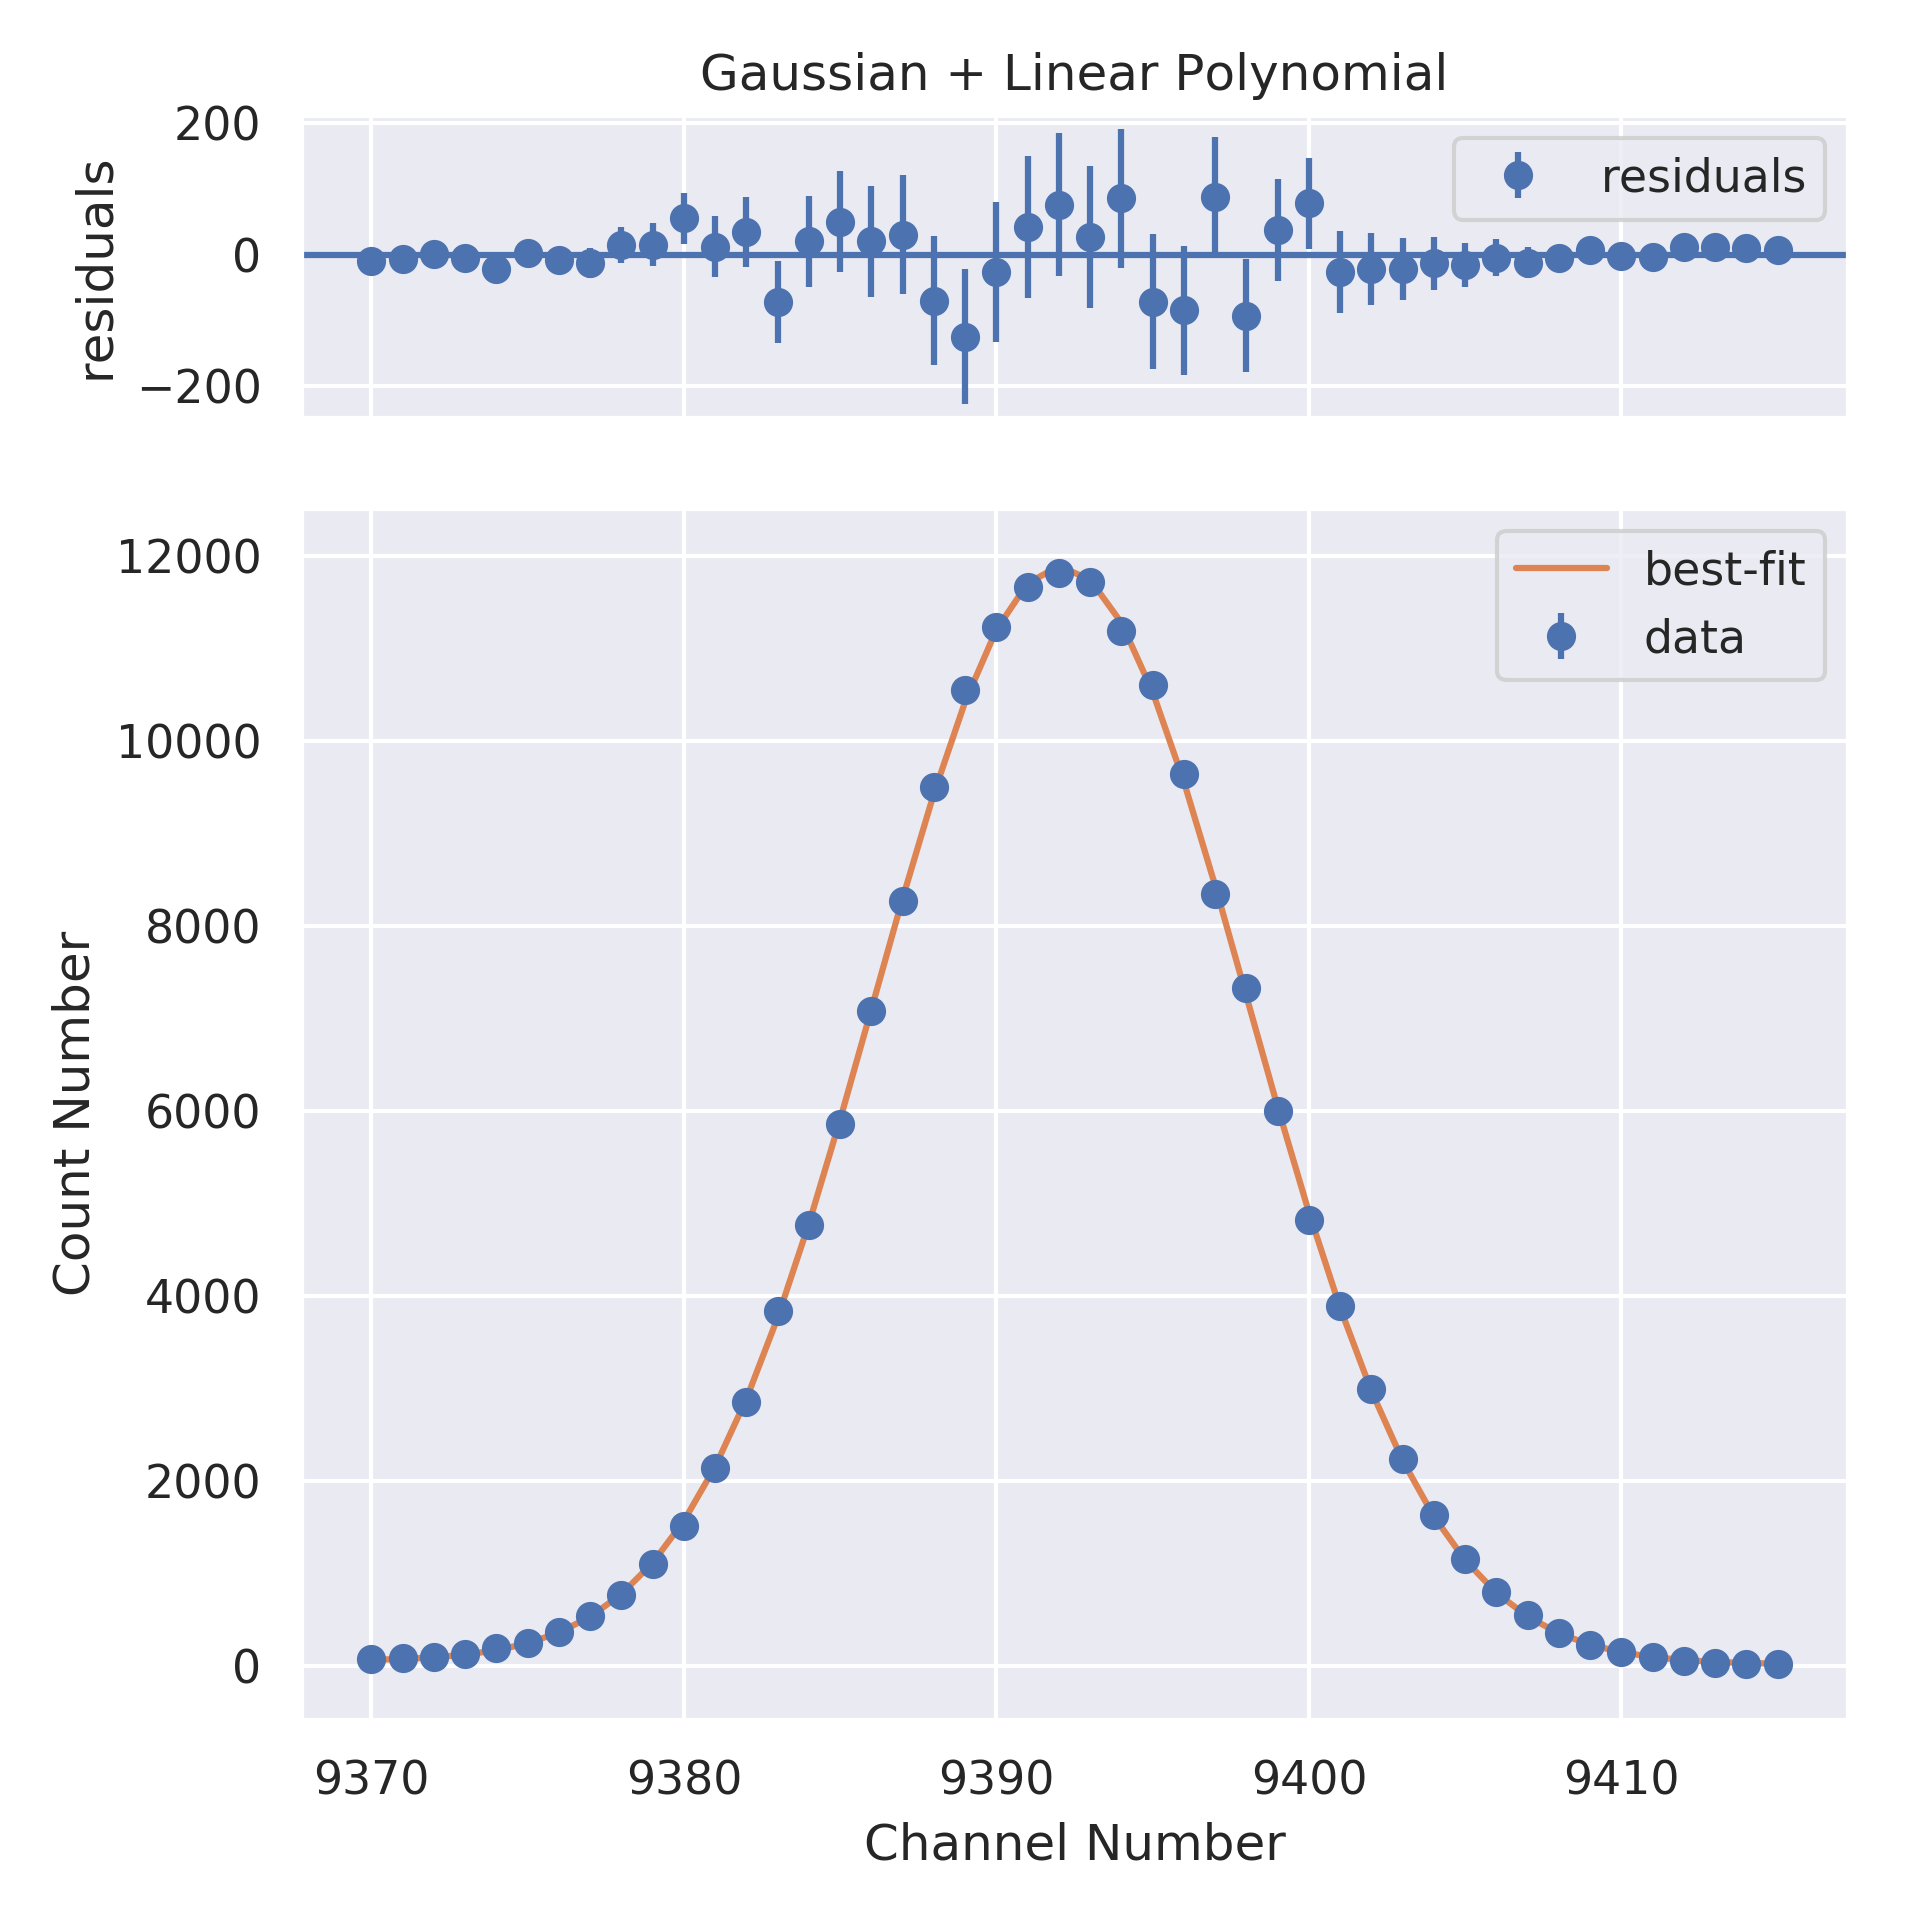
\includegraphics[width=\linewidth]{./Images/Cobalt60/Linear/Linear_2_Full.png}
    \caption{Full peak with fit}
    %\label{fig:sub1}
  \end{subfigure}%
  \begin{subfigure}{.5\linewidth}
    \centering
    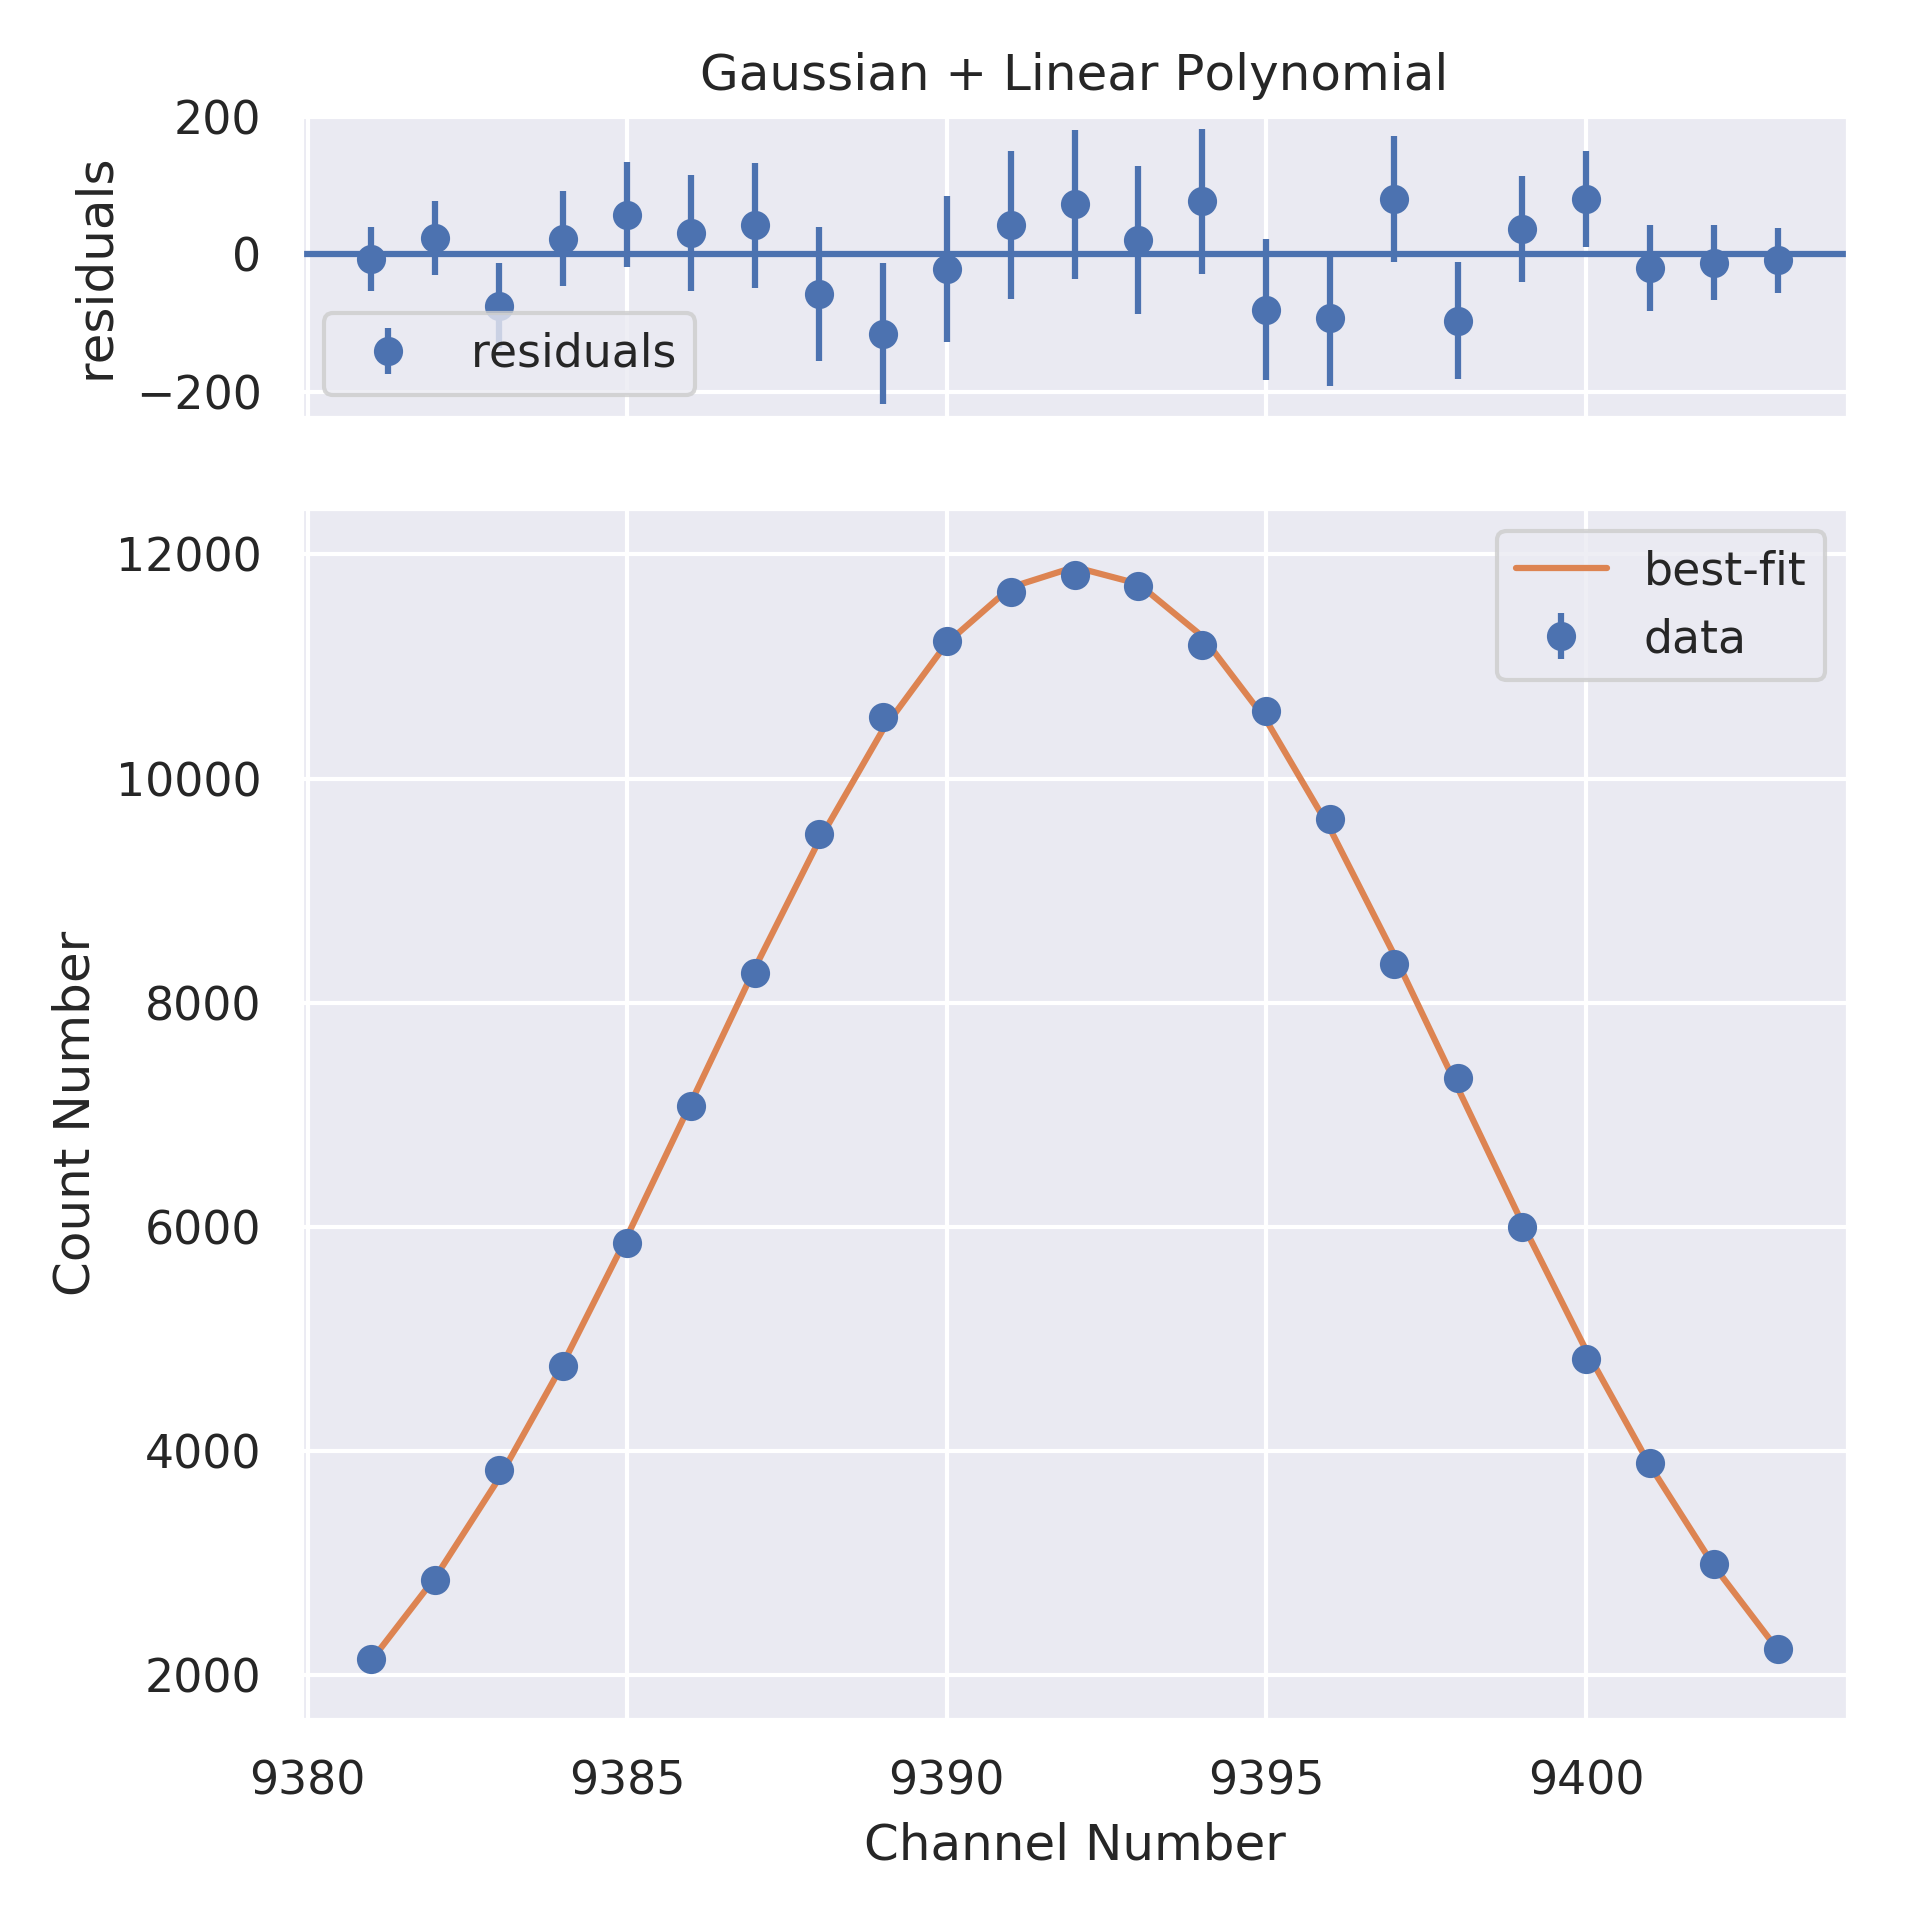
\includegraphics[width=\linewidth]{./Images/Cobalt60/Linear/Linear_2_Zoom.png}
    \caption{Zoomed in peak with fit}
    %\label{fig:sub2}
  \end{subfigure}
  \caption{Fit of full \& zoomed in peak of \element{Co}{60} 1332 keV peak}
  %\label{fig:test}
\end{figure}
\clearpage
\subsubsection{Quadratic + Gaussian Fit}
\begin{figure}[H]
  \centering
  \begin{subfigure}{.5\linewidth}
    \centering
    \includegraphics[width=\linewidth]{./Images/Cobalt60/Quad/Quad_1_Full.png}
    \caption{Full peak with fit}
    %\label{fig:sub1}
  \end{subfigure}%
  \begin{subfigure}{.5\linewidth}
    \centering
    \includegraphics[width=\linewidth]{./Images/Cobalt60/Quad/Quad_1_Zoom.png}
    \caption{Zoomed in peak with fit}
    %\label{fig:sub2}
  \end{subfigure}
  \caption{Fit of full \& zoomed in peak of \element{Co}{60} 1173 keV peak}
  %\label{fig:test}
\end{figure}
\begin{figure}[H]
  \centering
  \begin{subfigure}{.5\linewidth}
    \centering
    \includegraphics[width=\linewidth]{./Images/Cobalt60/Quad/Quad_2_Full.png}
    \caption{Full peak with fit}
    %\label{fig:sub1}
  \end{subfigure}%
  \begin{subfigure}{.5\linewidth}
    \centering
    \includegraphics[width=\linewidth]{./Images/Cobalt60/Quad/Quad_2_Zoom.png}
    \caption{Zoomed in peak with fit}
    %\label{fig:sub2}
  \end{subfigure}
  \caption{Fit of full \& zoomed in peak of \element{Co}{60} 1332 keV peak}
  %\label{fig:test}
\end{figure}
\clearpage
\subsection{Sodium-22}
\subsubsection{Gaussian Fit Only}
\begin{figure}[H]
  \centering
  \begin{subfigure}{.5\linewidth}
    \centering
    \includegraphics[width=\linewidth]{./Images/Sodium22/Gauss/Gauss_1_Full.png}
    \caption{Full peak with fit}
    %\label{fig:sub1}
  \end{subfigure}%
  \begin{subfigure}{.5\linewidth}
    \centering
    \includegraphics[width=\linewidth]{./Images/Sodium22/Gauss/Gauss_1_Zoom.png}
    \caption{Zoomed in peak with fit}
    %\label{fig:sub2}
  \end{subfigure}
  \caption{Fit of full \& zoomed in peak of \element{Na}{22} 511 keV peak}
  %\label{fig:test}
\end{figure}
\begin{figure}[H]
  \centering
  \begin{subfigure}{.5\linewidth}
    \centering
    \includegraphics[width=\linewidth]{./Images/Sodium22/Gauss/Gauss_2_Full.png}
    \caption{Full peak with fit}
    %\label{fig:sub1}
  \end{subfigure} 
  \begin{subfigure}{.5\linewidth}
    \centering
    \includegraphics[width=\linewidth]{./Images/Sodium22/Gauss/Gauss_2_Zoom.png}
    \caption{Zoomed in peak with fit}
    %\label{fig:sub2}
  \end{subfigure}
  \caption{Fit of full \& zoomed in peak of \element{Na}{22} 1274 keV peak}
  %\label{fig:test}
\end{figure}
\clearpage
\subsubsection{Linear + Gaussian Fit}
\begin{figure}[H]
  \centering
  \begin{subfigure}{.5\linewidth}
    \centering
    \includegraphics[width=\linewidth]{./Images/Sodium22/Linear/Linear_1_Full.png}
    \caption{Full peak with fit}
    %\label{fig:sub1}
  \end{subfigure}%
  \begin{subfigure}{.5\linewidth}
    \centering
    \includegraphics[width=\linewidth]{./Images/Sodium22/Linear/Linear_1_Zoom.png}
    \caption{Zoomed in peak with fit}
    %\label{fig:sub2}
  \end{subfigure}
  \caption{Fit of full \& zoomed in peak of \element{Na}{60} 511 keV peak}
  %\label{fig:test}
\end{figure}
\begin{figure}[H]
  \centering
  \begin{subfigure}{.5\linewidth}
    \centering
    \includegraphics[width=\linewidth]{./Images/Sodium22/Linear/Linear_2_Full.png}
    \caption{Full peak with fit}
    %\label{fig:sub1}
  \end{subfigure}%
  \begin{subfigure}{.5\linewidth}
    \centering
    \includegraphics[width=\linewidth]{./Images/Sodium22/Linear/Linear_2_Zoom.png}
    \caption{Zoomed in peak with fit}
    %\label{fig:sub2}
  \end{subfigure}
  \caption{Fit of full \& zoomed in peak of \element{Na}{22} 1274 keV peak}
  %\label{fig:test}
\end{figure}
\clearpage
\subsubsection{Quadratic + Gaussian Fit}
\begin{figure}[H]
  \centering
  \begin{subfigure}{.5\linewidth}
    \centering
    \includegraphics[width=\linewidth]{./Images/Sodium22/Quad/Quad_1_Full.png}
    \caption{Full peak with fit}
    %\label{fig:sub1}
  \end{subfigure}%
  \begin{subfigure}{.5\linewidth}
    \centering
    \includegraphics[width=\linewidth]{./Images/Sodium22/Quad/Quad_1_Zoom.png}
    \caption{Zoomed in peak with fit}
    %\label{fig:sub2}
  \end{subfigure}
  \caption{Fit of full \& zoomed in peak of \element{Na}{60} 511 keV peak}
  %\label{fig:test}
\end{figure}
\begin{figure}[H]
  \centering
  \begin{subfigure}{.5\linewidth}
    \centering
    \includegraphics[width=\linewidth]{./Images/Sodium22/Quad/Quad_2_Full.png}
    \caption{Full peak with fit}
    %\label{fig:sub1}
  \end{subfigure}%
  \begin{subfigure}{.5\linewidth}
    \centering
    \includegraphics[width=\linewidth]{./Images/Sodium22/Quad/Quad_2_Zoom.png}
    \caption{Zoomed in peak with fit}
    %\label{fig:sub2}
  \end{subfigure}
  \caption{Fit of full \& zoomed in peak of \element{Na}{22} 1274 keV peak}
  %\label{fig:test}
\end{figure}

\clearpage

\section{Fit Comparisons}
\subsection{Barium-133}

\begin{figure}[H]
  \centering
  \includegraphics[width=0.95\linewidth]{./Images/Barium133/FitComparison_Peak1.png}
  \caption{Fit comparisons for \element{Ba}{133} 81 keV peak}
\end{figure}

\begin{figure}[H]
  \centering
  \includegraphics[width=0.95\linewidth]{./Images/Barium133/FitComparison_Peak2.png}
  \caption{Fit comparisons for \element{Ba}{133} 161 keV peak}
\end{figure}

\begin{figure}[H]
  \centering
  \includegraphics[width=0.95\linewidth]{./Images/Barium133/FitComparison_Peak3.png}
  \caption{Fit comparisons for \element{Ba}{133} 223 keV peak}
\end{figure}

\begin{figure}[H]
  \centering
  \includegraphics[width=0.95\linewidth]{./Images/Barium133/FitComparison_Peak4.png}
  \caption{Fit comparisons for \element{Ba}{133} 276 keV peak}
\end{figure}

\begin{figure}[H]
  \centering
  \includegraphics[width=0.95\linewidth]{./Images/Barium133/FitComparison_Peak5.png}
  \caption{Fit comparisons for \element{Ba}{133} 303 keV peak}
\end{figure}

\begin{figure}[H]
  \centering
  \includegraphics[width=0.95\linewidth]{./Images/Barium133/FitComparison_Peak6.png}
  \caption{Fit comparisons for \element{Ba}{133} 356 keV peak}
\end{figure}

\begin{figure}[H]
  \centering
  \includegraphics[width=0.95\linewidth]{./Images/Barium133/FitComparison_Peak7.png}
  \caption{Fit comparisons for \element{Ba}{133} 384 keV peak}
\end{figure}
\clearpage

\subsection{Cobalt-60}

\begin{figure}[H]
  \centering
  \includegraphics[width=0.95\linewidth]{./Images/Cobalt60/FitComparison_Peak1.png}
  \caption{Fit comparisons for \element{Co}{60} 1173 keV peak}
\end{figure}

\begin{figure}[H]
  \centering
  \includegraphics[width=0.95\linewidth]{./Images/Cobalt60/FitComparison_Peak2.png}
  \caption{Fit comparisons for \element{Co}{60} 1332 keV peak}
\end{figure}
\clearpage

\subsection{Sodium-22}
\begin{figure}[H]
  \centering
  \includegraphics[width=0.95\linewidth]{./Images/Sodium22/FitComparison_Peak1.png}
  \caption{Fit comparisons for \element{Na}{22} 511 keV peak}
\end{figure}

\begin{figure}[H]
  \centering
  \includegraphics[width=0.95\linewidth]{./Images/Sodium22/FitComparison_Peak2.png}
  \caption{Fit comparisons for \element{Na}{22} 1274 keV peak}
\end{figure}
\clearpage

\section{Python Code}
\subsection{GaussianFit.py}

\begin{minted}[linenos,tabsize=2,breaklines,breakanywhere]{python}
import numpy as np
import matplotlib.pylab as plt
import seaborn as sns
sns.set()
import scipy.optimize as sciopt
import scipy.stats as scistats
from lmfit import Model, Parameters
import pandas as pd

def ChiSqFunc(Measured,Fitted,Errors):
  ChiSquared = 0
  for i in range(len(Measured)):
    ChiSquared += ((Measured[i] - Fitted[i])**2.0) / ((Errors[i])**2.0)
  ReducedChiSq = ChiSquared/(len(Measured)-2)
  ProbChiSq = (1.0 - scistats.chi2.cdf(ChiSquared,len(Measured)-2) )  * 100.0
  return ChiSquared, ReducedChiSq, ProbChiSq

def Gauss(x,A,mean,sigma,a):
  return (A/(np.sqrt(2*np.pi) * sigma )) *np.exp(-((x-mean)**2.0)/(2.0*(sigma**2.0))) + a

def GaussLinear(x,A,mean,sigma,a,b):
  return (A/(np.sqrt(2*np.pi) * sigma ))*np.exp(-((x-mean)**2.0)/(2.0*(sigma**2.0))) + a + b*x

def GaussQuad(x,A,mean,sigma,a,b,c):
  return (A/(np.sqrt(2*np.pi) * sigma ))*np.exp(-((x-mean)**2.0)/(2.0*(sigma**2.0))) + a + b*x + c*x**2.0    

def ChToEnergy(Ch,a,b,c):
  Energy = np.sqrt( ( (Ch - c + (b**2.0 / (4*a))) )/a ) - (b / (2*a))
  return Energy

SetSigma = 2

BariumList = [ [[550,585,570,81],[1125,1140,1132,161],[1565,1582,1574,223],[1935,1960,1948,276],[2118,2150,2135,303],[2493,2526,2509,356],[2688,2723,2705,384]] , [] ]
SodiumList = [ [ [3570,3630,3600,511] , [8966,9000,8984,1274]] , [] ]
CobaltList = [ [ [8250,8290,8270,1173] , [9370,9415,9392,1332]] , [] ]

SourceList = ["Barium133-24HrRun_006_eh_1","Sodium22-24HrData_002_eh_1","Cobalt60-24HrData_004_eh_1"]

PlotResolution = 300

PeakNo = int(1)

datadict = {'Element':[],'Fit type':[], 'Peak number':[], 'Peak type':[], 'Energy (keV)': [], 'Resolution':[], 'Min of range':[], 'Max of range':[], 'Mean':[], 'A':[], 'Sigma':[], 'Error on mean':[], 'a':[], 'b':[], 'c':[], 'chisq':[], 'Reduced chisq':[], 'Probchisq':[]}

# Fit parameters
a = 2.63977565e-06
b = 7.04767648
c = -1.91414134e-01

for source in SourceList:
  if source == "Barium133-24HrRun_006_eh_1":
    ElementList = BariumList
    Element = "Barium133"
  elif source == "Sodium22-24HrData_002_eh_1":
    ElementList = SodiumList
    Element = "Sodium22"
  else:
    ElementList = CobaltList
    Element = "Cobalt60"

  for item in ElementList:
    for peak in item:
      #! Initialises the source and ranges for run

      if item == ElementList[0]:
        PeakType = "Full"
      else:
        PeakType = "Zoom"

      df = pd.read_csv(source + ".dat", sep = r"\s+", names = ['channel number','count number'])

      df['count errors'] = np.sqrt(df['count number'])
      df['count errors'] = df['count errors'].replace(0,1)

      MinValue = peak[0]
      MaxValue = peak[1]
      MeanValue = peak[2]
      PeakEnergy = peak[3]

      data = df[(MinValue<=df['channel number']) & (df['channel number']<=MaxValue)]
      #?plt.plot(data['channel number'],data['count number'])
      #?plt.show()
      #----------------------------------------------------------------------------------------------------------
      #! Gaussian + Offset model only

      GaussModel = Model(Gauss)
      Params = Parameters()

      Params.add('A',value=max(data['count number']),vary=True,min=0)
      Params.add('mean',value=MeanValue,vary=True)
      Params.add('sigma',value=1,vary=True)
      Params.add('a',value=1,vary=True)

      FitResult = GaussModel.fit(data['count number'],params=Params,x=data['channel number'])
      TempList = [ FitResult.best_values['mean'] - SetSigma *FitResult.best_values['sigma'] , FitResult.best_values['mean'] + SetSigma *FitResult.best_values['sigma'] , FitResult.best_values['mean'] , PeakEnergy ] 
      if item == ElementList[0]:
        ElementList[1].append(TempList)
      #print(FitResult.best_values)
      FitResult.plot(yerr=data['count errors'],xlabel='Channel Number',ylabel='Count Number',title='Gaussian + Constant Offset')

      thingy = ChiSqFunc(list(data['count number']),list(FitResult.best_fit),list(data['count errors']))
      #print(thingy)

      #?plt.plot(data['channel number'],data['count number'])
      plt.tight_layout()
      plt.savefig(f'Plots/{Element}/Gauss/Gauss_{PeakNo}_{PeakType}.png', format='png', dpi=PlotResolution)
      plt.close('all')
      #plt.show()

      CountMax1 = FitResult.best_values['A'] / ( FitResult.best_values['sigma'] * np.sqrt(2 * np.pi ) ) + FitResult.best_values['a']
      ErrorOnMean1 = FitResult.best_values['sigma'] / np.sqrt(CountMax1)

      datadict['Element'].append(Element)
      datadict['Fit type'].append('Gauss')
      datadict['Energy (keV)'].append(PeakEnergy)
      FWHM_Energy = 2 * np.sqrt(2*np.log(2)) * ChToEnergy(FitResult.best_values['sigma'],a,b,c)
      datadict['Resolution'].append( FWHM_Energy / PeakEnergy)
      #datadict['Resolution'].append( ( (2 * np.sqrt(2*np.log(2))*FitResult.best_values['sigma'] - b ) / a ) / PeakEnergy)
      datadict['Peak number'].append(PeakNo)
      datadict['Peak type'].append(PeakType)
      datadict['Min of range'].append(MinValue)
      datadict['Max of range'].append(MaxValue)
      datadict['Mean'].append(FitResult.best_values['mean'])
      datadict['A'].append(FitResult.best_values['A'])
      datadict['Sigma'].append(FitResult.best_values['sigma'])
      datadict['Error on mean'].append(1)
      datadict['a'].append(FitResult.best_values['a'])
      datadict['b'].append(0)
      datadict['c'].append(0)
      datadict['chisq'].append(thingy[0])
      datadict['Reduced chisq'].append(thingy[1])
      datadict['Probchisq'].append(thingy[2])

      
      #----------------------------------------------------------------------------------------------------------
      #! Gaussain + Linear model 

      GaussModel2 = Model(GaussLinear)
      Params2 = Parameters()

      Params2.add('A',value=max(data['count number']),vary=True,min=0)
      Params2.add('mean',value=MeanValue,vary=True)
      Params2.add('sigma',value=1,vary=True)
      Params2.add('a',value=1,vary=True)
      Params2.add('b',value=1,vary=True)

      FitResult2 = GaussModel2.fit(data['count number'],params=Params2,x=data['channel number'])
      #TempList2 = [ FitResult2.best_values['mean'] - SetSigma *FitResult2.best_values['sigma'] , FitResult2.best_values['mean'] + SetSigma *FitResult2.best_values['sigma'] , FitResult2.best_values['mean']  ] 
      #print(FitResult2.best_values)
      FitResult2.plot(yerr=data['count errors'],xlabel='Channel Number',ylabel='Count Number',title='Gaussian + Linear Polynomial')

      thingy2 = ChiSqFunc(list(data['count number']),list(FitResult2.best_fit),list(data['count errors']))

      #?plt.plot(data['channel number'],data['count number'])
      plt.tight_layout()
      plt.savefig(f'Plots/{Element}/Linear/Linear_{PeakNo}_{PeakType}.png', format='png', dpi=PlotResolution)
      plt.close('all')

      CountMax2 = FitResult2.best_values['A'] / ( FitResult2.best_values['sigma'] * np.sqrt(2 * np.pi ) ) + FitResult2.best_values['a'] + FitResult2.best_values['b'] * FitResult2.best_values['mean']
      ErrorOnMean2 = FitResult2.best_values['sigma'] / np.sqrt(CountMax2)
      
      datadict['Element'].append(Element)
      datadict['Fit type'].append('Linear')
      datadict['Energy (keV)'].append(PeakEnergy)
      FWHM_Energy = 2 * np.sqrt(2*np.log(2)) * ChToEnergy(FitResult2.best_values['sigma'],a,b,c)
      datadict['Resolution'].append( FWHM_Energy / PeakEnergy)
      datadict['Peak number'].append(PeakNo)
      datadict['Peak type'].append(PeakType)
      datadict['Min of range'].append(MinValue)
      datadict['Max of range'].append(MaxValue)
      datadict['Mean'].append(FitResult2.best_values['mean'])
      datadict['A'].append(FitResult2.best_values['A'])
      datadict['Sigma'].append(FitResult2.best_values['sigma'])
      datadict['Error on mean'].append(1)
      datadict['a'].append(FitResult2.best_values['a'])
      datadict['b'].append(FitResult2.best_values['b'])
      datadict['c'].append(0)
      datadict['chisq'].append(thingy2[0])
      datadict['Reduced chisq'].append(thingy2[1])
      datadict['Probchisq'].append(thingy2[2])

      #----------------------------------------------------------------------------------------------------------
      #! Gaussain + Quadratic model 

      GaussModel3 = Model(GaussQuad)
      Params3 = Parameters()

      Params3.add('A',value=max(data['count number']),vary=True,min=0)
      Params3.add('mean',value=MeanValue,vary=True)
      Params3.add('sigma',value=1,vary=True)
      Params3.add('a',value=1,vary=True)
      Params3.add('b',value=1,vary=True)
      Params3.add('c',value=1,vary=True)

      FitResult3 = GaussModel3.fit(data['count number'],params=Params3,x=data['channel number'])
      #TempList3 = [ FitResult3.best_values['mean'] - SetSigma *FitResult3.best_values['sigma'] , FitResult3.best_values['mean'] + SetSigma *FitResult3.best_values['sigma'] , FitResult3.best_values['mean']  ] 
      #print(FitResult3.best_values)
      FitResult3.plot(yerr=data['count errors'],xlabel='Channel Number',ylabel='Count Number',title='Gaussian + Quadratic Polynomial')

      thingy3 = ChiSqFunc(list(data['count number']),list(FitResult3.best_fit),list(data['count errors']))
      #print(thingy3)

      #?plt.plot(data['channel number'],data['count number'])
      plt.tight_layout()
      plt.savefig(f'Plots/{Element}/Quad/Quad_{PeakNo}_{PeakType}.png', format='png', dpi=PlotResolution)
      plt.close('all')

      CountMax3 = FitResult3.best_values['A'] / ( FitResult3.best_values['sigma'] * np.sqrt(2 * np.pi ) ) + FitResult3.best_values['a'] + FitResult3.best_values['b'] * FitResult3.best_values['mean'] + FitResult3.best_values['c'] * (FitResult3.best_values['mean'])** 2.0
      ErrorOnMean3 = FitResult3.best_values['sigma'] / np.sqrt(CountMax3)

      datadict['Element'].append(Element)
      datadict['Fit type'].append('Quad')
      datadict['Energy (keV)'].append(PeakEnergy)
      FWHM_Energy = 2 * np.sqrt(2*np.log(2)) * ChToEnergy(FitResult3.best_values['sigma'],a,b,c)
      datadict['Resolution'].append( FWHM_Energy / PeakEnergy)
      datadict['Peak number'].append(PeakNo)
      datadict['Peak type'].append(PeakType)
      datadict['Min of range'].append(MinValue)
      datadict['Max of range'].append(MaxValue)
      datadict['Mean'].append(FitResult3.best_values['mean'])
      datadict['A'].append(FitResult3.best_values['A'])
      datadict['Sigma'].append(FitResult3.best_values['sigma'])
      datadict['Error on mean'].append(1)
      datadict['a'].append(FitResult3.best_values['a'])
      datadict['b'].append(FitResult3.best_values['b'])
      datadict['c'].append(FitResult3.best_values['c'])
      datadict['chisq'].append(thingy3[0])
      datadict['Reduced chisq'].append(thingy3[1])
      datadict['Probchisq'].append(thingy3[2])
      

      Delta12 = np.abs(FitResult.best_values['mean'] - FitResult2.best_values['mean'])
      ErrorDelta12 = np.sqrt( ErrorOnMean1**2.0 + ErrorOnMean2**2.0 )

      Delta23 = np.abs(FitResult2.best_values['mean'] - FitResult3.best_values['mean'])
      ErrorDelta23 = np.sqrt( ErrorOnMean2**2.0 + ErrorOnMean3**2.0 )


      if PeakType == "Zoom":
        if abs(ErrorDelta23) > abs(Delta23):
          print('best fit')
        else:
          print('not best fit')
            
        TitleFont = {'size':'24', 'color':'black', 'weight':'bold'} 
        AxTitleFont = {'size':'16'}
        plt.figure(figsize=(10,6))
        plt.errorbar(FitResult.best_values['mean'],1,xerr=ErrorOnMean1,elinewidth=6,capsize=10,capthick=5,marker='o',markersize=20,label="Gauss")
        plt.errorbar(FitResult2.best_values['mean'],1.25,xerr=ErrorOnMean2,elinewidth=6,capsize=10,capthick=5,marker='o',markersize=20,label="GaussLinear")
        plt.errorbar(FitResult3.best_values['mean'],1.5,xerr=ErrorOnMean3,elinewidth=6,capsize=10,capthick=5,marker='o',markersize=20,label="GaussQuad")
        plt.legend(fontsize=16,markerscale=0.33)
        plt.title(str(Element) + ' Peak Number ' + str(PeakNo),**TitleFont)
        plt.xlabel('Channel Numbers',**AxTitleFont)
        plt.yticks([1,1.25,1.5],['Guass','GuassLinear','GaussQuad'],**AxTitleFont)
        plt.tight_layout()
        plt.savefig(f'Plots/{Element}/FitComparison_Peak{PeakNo}.png', format='png', dpi=PlotResolution)
        plt.close('all')
      
      PeakNo +=1

    PeakNo = 1

Fitdf = pd.DataFrame(datadict)
Fitdf.to_csv('Gamma_Peak_Stats_and_Params.csv')
\end{minted}

\clearpage
\subsection{Calibration.py}

\begin{minted}[linenos,tabsize=2,breaklines,breakanywhere]{python}
import numpy as np
import matplotlib.pyplot as plt
import scipy.optimize as sciopt
import seaborn as sns
import pandas as pd
sns.set()
import scipy.stats as scistats

source = "MysterySource-2HrRun_001_eh_1"
df = pd.read_csv(source+ ".dat", sep=r"\s+",names = ['channel number','count number'])

TitleFont = {'size':'25', 'color':'black', 'weight':'bold'} 
AxTitleFont = {'size':'22'}

def Linear(E,a,b):
    return E*a + b

def Quadratic(E,a,b,c):
    return a*E**2.0 + E*b + c

def ChiSqFunc(Measured,Fitted,Errors,Params):
  ChiSquared = 0
  for i in range(len(Measured)):
    ChiSquared += ((Measured[i] - Fitted[i])**2.0) / ((Errors[i])**2.0)
  ReducedChiSq = ChiSquared/(len(Measured)-len(Params))
  ProbChiSq = (1.0 - scistats.chi2.cdf(ChiSquared,len(Measured)-len(Params)) )  * 100.0
  return ChiSquared, ReducedChiSq, ProbChiSq


FitDF = pd.read_csv('Gamma_Peak_Stats_and_Params.csv', names=['Element', 'Fit type', 'Peak number',	'Peak type', 'Energy (keV)', 'Resolution', 'Min', 'Max', 'Mean', 'A', 'Sigma', 'Error' ,'a', 'b', 'chisq', 'Reduced chisq', 'Probchisq'],usecols=list(range(1,18)))

FitDF = FitDF[FitDF['Fit type'] == 'Linear']
FitDF = FitDF[FitDF['Peak type'] == 'Zoom']

FitDF['Mean'] = FitDF['Mean'].astype(float)
FitDF['Error'] = FitDF['Error'].astype(float)

FitDF['Energy (keV)'] = FitDF['Energy (keV)'].astype(float)

plt.plot(FitDF['Energy (keV)'],FitDF['Mean'],'bo')

plt.show()

DataBa = FitDF[FitDF['Element'] == 'Barium133']
DataCo = FitDF[FitDF['Element'] == 'Cobalt60']
DataNa = FitDF[FitDF['Element'] == 'Sodium22']


ParamsLinear, ErrorsLinear = sciopt.curve_fit(Quadratic,FitDF['Energy (keV)'],FitDF['Mean'])
print(ParamsLinear)

rough_EC_a = a = ParamsLinear[0]
rough_EC_b = b = ParamsLinear[1]
rough_EC_c = c = ParamsLinear[2]


Energies = np.sqrt( (FitDF['Mean'] - c + (b**2.0/ (4 * a)))/a ) - (b/(2*a))

plt.errorbar(DataBa['Energy (keV)'],DataBa['Mean'], fmt='ro',label="Barium-133", markersize=10.5,yerr=DataBa['Error'].values)
plt.errorbar(DataCo['Energy (keV)'],DataCo['Mean'],fmt='bo',label="Cobalt-60", markersize=10.5,yerr=DataCo['Error'].values)
plt.errorbar(DataNa['Energy (keV)'],DataNa['Mean'],fmt='yo',label="Sodium-22", markersize=10.5,yerr=DataNa['Error'].values)

plt.plot(Energies,Quadratic(Energies,*ParamsLinear),label='Fit')
plt.title('Energy calibration plot with fit',**TitleFont)
plt.xlabel('Gamma Energy [keV]',**AxTitleFont)
plt.ylabel('Channel Number',**AxTitleFont)
plt.legend()
plt.show()


plt.errorbar(DataBa['Energy (keV)'],[(DataBa['Mean'].iloc[i] - Quadratic(DataBa['Energy (keV)'].iloc[i],*ParamsLinear)) for i in range(len(DataBa['Energy (keV)']))],fmt='ro',label="Barium-133", markersize=7.5,yerr=DataBa['Error'].values)
plt.errorbar(DataCo['Energy (keV)'],[(DataCo['Mean'].iloc[i] - Quadratic(DataCo['Energy (keV)'].iloc[i],*ParamsLinear)) for i in range(len(DataCo['Energy (keV)']))],fmt='bo',label="Cobalt-60", markersize=7.5,yerr=DataCo['Error'].values)
plt.errorbar(DataNa['Energy (keV)'],[(DataNa['Mean'].iloc[i] - Quadratic(DataNa['Energy (keV)'].iloc[i],*ParamsLinear)) for i in range(len(DataNa['Energy (keV)']))],fmt='yo',label="Sodium-22", markersize=7.5,yerr=DataNa['Error'].values)
plt.title('Energy calibration residual plot',**TitleFont)
plt.xlabel('Gamma Energy [keV]',**AxTitleFont)
plt.ylabel('Channel Number Residual',**AxTitleFont)
plt.legend()
plt.show()


ChiStats = ChiSqFunc(list(FitDF['Mean']),list(Quadratic(FitDF['Energy (keV)'],*ParamsLinear)),list(FitDF['Error']),ParamsLinear)
print(ChiStats)
\end{minted}
\clearpage

\subsection{Subtraction.py}
\begin{minted}[linenos,tabsize=2,breaklines,breakanywhere]{python}
import numpy as np
import matplotlib.pyplot as plt
import seaborn as sns
sns.set()
import scipy as sc
import pandas as pd

# If statements that control what the code does! 
PlotMysterySource = True
PlotKnownSources = True

# Plot controlls
TitleFont = {'size':'23', 'color':'black', 'weight':'bold'} 
AxTitleFont = {'size':'20'}

if PlotMysterySource:
	BgWithShield = "WeekendBgWithShield_003_eh_1"
	BgWithShieldDF = pd.read_csv(BgWithShield+ ".dat", sep=r"\s+",names = ['channel number','count number'])
	
	MysterySource = "MysterySource-24HrRun_001_eh_1"
	MysterySourceDF = pd.read_csv(MysterySource+ ".dat", sep=r"\s+",names = ['channel number','count number'])
	
	# Normalises the timings of the two runs to 24 hours each
	BgWithShieldDF['count number2'] = BgWithShieldDF['count number'] 
	BgWithShieldDF['count number'] = BgWithShieldDF['count number'] / ( 239068  ) * 86400
	
	MysterySourceDF['count number'] = MysterySourceDF['count number'] - BgWithShieldDF['count number']
	
	a = 2.63977565e-06
	b = 7.04767648
	c = -1.91414134e-01

	MysterySourceDF['Energies'] =  np.sqrt( (BgWithShieldDF['channel number'] - c + (b**2.0/ (4 * a)))/a ) - (b/(2*a))
	BgWithShieldDF['Energies'] =  np.sqrt( (BgWithShieldDF['channel number'] - c + (b**2.0/ (4 * a)))/a ) - (b/(2*a))

	
	plt.semilogy(MysterySourceDF['Energies'],MysterySourceDF['count number'],label="Mystery Source")
	plt.semilogy(BgWithShieldDF['Energies'],BgWithShieldDF['count number2'],label="Background With Shield")
	plt.xlabel('Gamma Energy [keV]',**AxTitleFont)
	plt.ylabel('Log-10 of count number',**AxTitleFont)
	plt.title('Mystery Source With Background Subtracted',**TitleFont)
	plt.xlim(0,2216)
	plt.ylim(1)
	plt.legend()
	plt.show()


if PlotKnownSources:
	BgWithShield = "WeekendBgWithShield_003_eh_1"
	BgWithShieldDF = pd.read_csv(BgWithShield+ ".dat", sep=r"\s+",names = ['channel number','count number'])
	
	Sodium = 'Sodium22-24HrData_002_eh_1'
	SodiumDF = pd.read_csv(Sodium+ ".dat", sep=r"\s+",names = ['channel number','count number'])
	
	Barium = 'Barium133-24HrRun_006_eh_1'
	BariumDF = pd.read_csv(Barium+ ".dat", sep=r"\s+",names = ['channel number','count number'])
	
	Cobalt = 'Cobalt60-24HrData_004_eh_1'
	CobaltDF = pd.read_csv(Cobalt+ ".dat", sep=r"\s+",names = ['channel number','count number'])
	
	# Normalises the background to the correct timings
	BgWithShieldDFCobalt = BgWithShieldDF.copy()
	BgWithShieldDF['count number'] = BgWithShieldDF['count number'] / ( 239068  ) * 86400
	BgWithShieldDFCobalt['count number'] = BgWithShieldDF['count number'] / ( 239068  ) * (86400/12.0)
	
	# Subtracts the background from the original data
	SodiumDF['count number'] = SodiumDF['count number'] - BgWithShieldDF['count number']
	BariumDF['count number'] = BariumDF['count number'] - BgWithShieldDF['count number']
	CobaltDF['count number'] = CobaltDF['count number'] - BgWithShieldDFCobalt['count number']
		
	# Fitting parameters
	a = 7.01164642
	b = 8.1697501	
	
	# Converting channel numbers to energies
	SodiumDF['Energies'] = ( SodiumDF['channel number'] - b )/a
	BariumDF['Energies'] = ( BariumDF['channel number'] - b )/a
	CobaltDF['Energies'] = ( CobaltDF['channel number'] - b )/a
	
	
	# Now plotting the different elements on different log-y plots.
	
	plt.figure(1)
	plt.semilogy(SodiumDF['Energies'],SodiumDF['count number'],label="Sodium 22 data",color='yellow')
	TitleFont = {'size':'25', 'color':'black', 'weight':'bold'} 
	AxTitleFont = {'size':'22'}
	plt.xlabel('Gamma Energy [keV]',**AxTitleFont)
	plt.ylabel('Log-10 of count number',**AxTitleFont)
	plt.title('Sodium 22, no background, energies',**TitleFont)
	plt.xlim(0)
	plt.ylim(1)
	plt.legend()


	plt.figure(2)
	plt.semilogy(BariumDF['Energies'],BariumDF['count number'],label="Barium 133 data",color='green')
	TitleFont = {'size':'25', 'color':'black', 'weight':'bold'} 
	AxTitleFont = {'size':'22'}
	plt.xlabel('Gamma Energy [keV]',**AxTitleFont)
	plt.ylabel('Log-10 of count number',**AxTitleFont)
	plt.title('Barium 133, no background, energies',**TitleFont)
	plt.xlim(0)
	plt.ylim(1)
	plt.legend()


	plt.figure(3)
	plt.semilogy(CobaltDF['Energies'],CobaltDF['count number'],label="Cobalt 60 data",color='blue')
	TitleFont = {'size':'25', 'color':'black', 'weight':'bold'} 
	AxTitleFont = {'size':'22'}
	plt.xlabel('Gamma Energy [keV]',**AxTitleFont)
	plt.ylabel('Log-10 of count number',**AxTitleFont)
	plt.title('Cobalt 60, no background, energies',**TitleFont)
	plt.xlim(0)
	plt.ylim(1)
	plt.legend()
	plt.show()
\end{minted}
\clearpage

\subsection{Resolution.py}
\begin{minted}[linenos,tabsize=2,breaklines,breakanywhere]{python}
import numpy as np
import matplotlib.pyplot as plt
import scipy.optimize as sciopt
import seaborn as sns
import pandas as pd
sns.set()
import scipy.stats as scistats


def ResolutionFit(E,a,b):
  return a/np.sqrt(E) + b

FitDF = pd.read_csv('Gamma_Peak_Stats_and_Params.csv', names=['Element', 'Fit type', 'Peak number',	'Peak type', 'Energy (keV)', 'Resolution', 'Min', 'Max', 'Mean', 'A', 'Sigma', 'Error' ,'a', 'b', 'chisq', 'Reduced chisq', 'Probchisq'],usecols=list(range(1,18)))

FitDF = FitDF[FitDF['Fit type'] == 'Linear']
FitDF = FitDF[FitDF['Peak type'] == 'Zoom']

FitDF['Energy (keV)'] = FitDF['Energy (keV)'].astype(float)
FitDF['Resolution'] = FitDF['Resolution'].astype(float).multiply(100)
SodiumDF = FitDF[(FitDF['Energy (keV)'] == 511)]
FitDF = FitDF[~(FitDF['Energy (keV)'] == 511)]


DataBa = FitDF[FitDF['Element'] == 'Barium133']
DataCo = FitDF[FitDF['Element'] == 'Cobalt60']
DataNa = FitDF[FitDF['Element'] == 'Sodium22']


Fit, Errors = sciopt.curve_fit(ResolutionFit,FitDF['Energy (keV)'],FitDF['Resolution'])
print(Fit)

TitleFont = {'size':'20', 'color':'black', 'weight':'bold'} 
AxTitleFont = {'size':'18'}

plt.figure(1)
Energies = np.linspace(55,1400,14000)
plt.plot(Energies,ResolutionFit(Energies,*Fit),label="Fit")

plt.errorbar(DataBa['Energy (keV)'],DataBa['Resolution'],fmt="o",color='red',label="Barium-133",markersize=7,yerr=(7.05/DataBa['Energy (keV)']),elinewidth=3,capsize=5,capthick=3,marker='o')
plt.errorbar(DataCo['Energy (keV)'],DataCo['Resolution'],fmt="o",color='blue',label="Cobalt-60",markersize=7,yerr=(7.05/DataCo['Energy (keV)']),elinewidth=3,capsize=5,capthick=3,marker='o')
plt.errorbar(DataNa['Energy (keV)'],DataNa['Resolution'],fmt="o",color='yellow',label="Sodium-22",markersize=7,yerr=(7.05/DataNa['Energy (keV)']),elinewidth=3,capsize=5,capthick=3,marker='o')
plt.errorbar(SodiumDF['Energy (keV)'],SodiumDF['Resolution'],fmt="o",color='yellow',label="",markersize=7,yerr=(7.05/SodiumDF['Energy (keV)']),elinewidth=3,capsize=5,capthick=3,marker='o')
plt.xlabel('Peak Energy [keV]',**AxTitleFont)
plt.ylabel('Energy Resolution [%]',**AxTitleFont)
plt.title('Energy Resolution as a Function of Gamma Energy',**TitleFont)
plt.legend(fontsize=16,fancybox=True,shadow=False)

plt.figure(2)
plt.errorbar(DataBa['Energy (keV)'],DataBa['Resolution']-ResolutionFit(DataBa['Energy (keV)'],*Fit),fmt="o",color='red',label="Barium-133",markersize=7,yerr=(7.05/DataBa['Energy (keV)']),elinewidth=3,capsize=5,capthick=3,marker='o')
plt.errorbar(DataCo['Energy (keV)'],DataCo['Resolution']-ResolutionFit(DataCo['Energy (keV)'],*Fit),fmt="o",color='blue',label="Cobalt-60",markersize=7,yerr=(7.05/DataCo['Energy (keV)']),elinewidth=3,capsize=5,capthick=3,marker='o')
plt.errorbar(DataNa['Energy (keV)'],DataNa['Resolution']-ResolutionFit(DataNa['Energy (keV)'],*Fit),fmt="o",color='yellow',label="Sodium-22",markersize=7,yerr=(7.05/DataNa['Energy (keV)']),elinewidth=3,capsize=5,capthick=3,marker='o')
plt.errorbar(SodiumDF['Energy (keV)'],SodiumDF['Resolution']-ResolutionFit(SodiumDF['Energy (keV)'],*Fit),fmt="o",color='yellow',label="",markersize=7,yerr=(7.05/SodiumDF['Energy (keV)']),elinewidth=3,capsize=5,capthick=3,marker='o')
plt.xlabel('Peak Energy [keV]',**AxTitleFont)
plt.ylabel('Energy Resolution Residual [%]',**AxTitleFont)
plt.title('Energy Resolution Residuals',**TitleFont)
plt.legend(fontsize=16,fancybox=True,shadow=False)
plt.show()

def ChiSqFunc(Measured,Fitted,Errors,Params):
  ChiSquared = 0
  for i in range(len(Measured)):
    ChiSquared += ((Measured[i] - Fitted[i])**2.0) / ((Errors[i])**2.0)
  ReducedChiSq = ChiSquared/(len(Measured)-len(Params))
  ProbChiSq = (1.0 - scistats.chi2.cdf(ChiSquared,len(Measured)-len(Params)) )  * 100.0
  return ChiSquared, ReducedChiSq, ProbChiSq


MeasuredThungys = list(DataBa['Resolution'])+list(DataCo['Resolution']) + list(DataNa['Resolution'])
FittedThingys = list(ResolutionFit(DataBa['Energy (keV)'],*Fit)) + list(ResolutionFit(DataCo['Energy (keV)'],*Fit)) + list(ResolutionFit(DataNa['Energy (keV)'],*Fit))
ErrorThingys = list(7.05/DataBa['Energy (keV)']) + list(7.05/DataCo['Energy (keV)']) + list(7.05/DataBa['Energy (keV)'])

ChiStats = ChiSqFunc(MeasuredThungys, FittedThingys, ErrorThingys,Fit)
print(ChiStats)
\end{minted}



\end{document}
